% ================================================================================
% IPEMToolboxManual.tex
% Main TeX file for the Manual of the IPEM Toolbox
% ================================================================================

% --------------------------------------------------------------------------------
% Use the following line(s) to include only (a) specific part(s) of the document
% (place a % sign in front of it to include everything)
%
%\includeonly{ReferenceManualIntroduction}
%\includeonly{ReferenceManualFunctionReference}
%\includeonly{AppRoughnessExperiments}
%\includeonly{AppTonalityInductionExperiments}
%\includeonly{AppRhythmicPatternExtraction}
%\includeonly{RhythmModule}

% --------------------------------------------------------------------------------

% --------------------------------------------------------------------------------
% Start of preamble - don't change these settings please...
%                     (except for setting the defined IPEMFlag... variables)
% --------------------------------------------------------------------------------

% Setup document style and formatting
\documentclass[a4paper,oneside,12pt]{book}
\setlength{\parindent}{0pt} \addtolength{\hoffset}{-50pt}
\addtolength{\textwidth}{105pt} \addtolength{\voffset}{-40pt}
\addtolength{\textheight}{60pt}

% Include support for conditionals
\usepackage{ifthen}

% Define some flags
\newboolean{IPEMFlagPDFOutput} % true for PDF output, false otherwise (dvips)
\newboolean{IPEMFlagGraphics} % true when you want to include graphics, false otherwise

% Set document flags
\setboolean{IPEMFlagPDFOutput}{true} % true or false
\setboolean{IPEMFlagGraphics}{true} % true or false

% Include support for graphics
\ifthenelse{\boolean{IPEMFlagPDFOutput}}
{ \ifthenelse{\boolean{IPEMFlagGraphics}}
    {\usepackage[pdftex]{graphicx}}
    {\usepackage[pdftex,draft]{graphicx}}
} {\ifthenelse{\boolean{IPEMFlagGraphics}}
    {\usepackage[dvips]{graphicx}}
    {\usepackage[dvips,draft]{graphicx}}
}

% Include support for hyper references
% (should be last in the list of included packages according to its documentation,
% but in practice it only works together with the apacite package when it's placed
% in front of that package)
\usepackage[backref=true,urlcolor=blue,linkcolor=red,colorlinks=true]{hyperref}

% Include support for citations
\usepackage{apacite}

% Self-defined commands and environments
\newcommand{\IPEMMailSupport}{\href{mailto:toolbox[at]ipem[dot]ugent[dot]be}{toolbox[at]ipem[dot]ugent[dot]be}}
\newcommand{\IPEMWebSite}[1]{\href{http://www.ipem.ugent.be#1}{www.ipem.ugent.be#1}}
\newcommand{\IPEMTBC}{\begin{large} \textit{... To Be Completed ...} \end{large}}
\newcommand{\IPEMVersion}{Version: 1.02 (beta)}
\newcommand{\IPEMDate}{Date: 20140106}
\newcommand{\IPEMDefaultFigureWidth}{12cm}
\newcommand{\IPEMCodeExtract}[1]{\texttt{\normalsize{#1}}}
\newenvironment{IPEMCodeEnvironment}{ \begin{ttfamily} \begin{small} }{ \end{small} \end{ttfamily} }
\newcommand{\IPEMShortTitle}{IPEM Toolbox}
\newcommand{\IPEMFullTitle}{Toolbox for perception-based music analysis}
\newcommand{\IPEMAuthors}{Marc Leman, Micheline Lesaffre, Koen Tanghe}

% Better layout
\usepackage{fancyhdr}
\pagestyle{fancy}
\fancyhead{}
\fancyhead[L]{\color[gray]{0.4}\slshape\leftmark}
\fancyhead[R]{\color[gray]{0.4}\slshape\rightmark}
\fancyfoot[L]{\color[gray]{0.4}\slshape{IPEM Toolbox Manual}}
\fancyfoot[C]{\color[gray]{0.4}}
\fancyfoot[R]{\color[gray]{0.4}\slshape\thepage}
\renewcommand{\headrulewidth}{0.4pt}
\renewcommand{\footrulewidth}{0.4pt}
\renewcommand{\chaptermark}[1]{\markboth{\MakeUppercase{Chapter \thechapter \ - #1}}{}}
\renewcommand{\sectionmark}[1]{\markright{#1}}
\addtolength{\headheight}{\baselineskip} %2.5pt}

% Include support for tables
\usepackage{tabularx}

% \IPEMSound{inSoundFile}{inText}
% Command for inserting a link to an external sound file:
% - inSoundFile = path\name of sound file (with path relative to document location)
% - inText = text for the link
\newlength{\IPEMCharHeight}
\ifthenelse{\boolean{IPEMFlagPDFOutput}}
    {   \newcommand{\IPEMSound}[2]{\settoheight{\IPEMCharHeight}{L}\pdfstartlink user{
                /Subtype /Movie
                /Movie<</Type/Sound/F(#1)>>
                /Border [0 0 0]
            }#2 
\includegraphics[height=\IPEMCharHeight]{Graphics/Ear}\pdfendlink
        }
    }
    {   \newcommand{\IPEMSound}[2] % otherwise, a hyperlink is used
        {\href{#1}{#2}}
    }

% Include PDF file information
\ifthenelse{\boolean{IPEMFlagPDFOutput}}
    {   \pdfinfo
        {   /Title      (\IPEMShortTitle: \IPEMFullTitle)
            /Author     (\IPEMAuthors)
            /Subject    (Manual for \IPEMShortTitle)
            /Keywords   (auditory processing,music analysis,perception,MATLAB)
        }
    }
    {}


% --------------------------------------------------------------------------------
% End of preamble
% --------------------------------------------------------------------------------


\begin{document}

\bibliographystyle{apacite}

\begin{titlepage}
    \begin{center}
        
\includegraphics[width=5cm]{Graphics/IpemLogo}
        \\[3cm]
        \textbf{\Huge \IPEMFullTitle}
        \\[0.8cm]
        \textbf{\LARGE Concepts, demos, and reference manual}
        \\[1.5cm]

        \IPEMAuthors\\
        Institute for Psychoacoustics and Electronic Music (IPEM)\\
        Ghent University\\
        Blandijnberg 2\\
        9000 Ghent, Belgium\\
        \IPEMMailSupport\\
        \IPEMWebSite{}\\[1.5cm]

        \IPEMVersion\\
        \IPEMDate
        \\[1.5cm]

    \end{center}
\end{titlepage}


\newpage
% --------------------------------------------------------------------------------
% Copyright notice FDL
% --------------------------------------------------------------------------------

\begin{quote}
    Copyright \copyright  2014 Ghent University\\
    Permission is granted to copy, distribute and/or modify this document
    under the terms of the GNU Free Documentation License, Version 1.2
    or any later version published by the Free Software Foundation;
    with no Invariant Sections, no Front-Cover Texts, and no Back-Cover Texts.
    A copy of the license is included in the section entitled
    "\hyperlink{ReferenceManual:GNUFreeDocumentationLicense}{GNU Free Documentation
    License}".
\end{quote}


\tableofcontents

\newpage
\part{Introduction}
\hypertarget{Part:Introduction}{}
% --------------------------------------------------------------------------------
% Introduction
% --------------------------------------------------------------------------------

\newpage
% --------------------------------------------------------------------------------
% Introduction: Introduction
% --------------------------------------------------------------------------------

\chapter*{\IPEMFullTitle}
\hypertarget{Chapter:IntroductionIntroduction}{}

\section*{Our motivation}
The motivation for developing a toolbox for perception-based
music analysis starts from the observation that much of the world
music production (seen over different cultures and time periods)
has no score representation, and that if a score representation is
available, it still represents but a small percentage of what
musical communication really is about. A sonological analysis of
musical sounds may provide steps towards a better understanding
of the components that contribute to musical information
processing but is also insufficient in view of how humans deal
with musical signals.

Up to the 19th century, the score was indeed the main carrier for
musical representation. And as a consequence musicology had a
focus on pitch and duration analysis, the main musical parameters
to encode in scores. But in the 20th century, thanks to the
breakthrough of electronic means for music production and
analysis, more powerful devices allowed for the control of
physical aspects of music. New methods for musical sound analysis
have been developed and the focus on pitch has been extended
towards timbre and sound effects. By the end of the 20th century,
digital technology laid the foundation for computer modeling of
perception and cognition, thereby offering a global human
information processing approach to music analysis. In this
approach aspects of musical communication that are based on pitch,
timbre, texture, expression, spatialization etc... can be studied
in close connection with empirical based scientific disciplines.

Technology has revolutionized our conception of what kind of music
research will be possible in the 21st century. But it is the task
of musicologists, in collaboration with other scientists, such as
engineers, psychologists, and brain scientists, to make these
dreams more concrete. Our basic motivation for developing this
toolbox is a \emph{pragmatic} one: if the musicology aims at
understanding music as a social and cultural phenomenon embedded
in the physical world and mediated through human faculties of
perception, cognition, and processing of expressive communication,
then new tools must be developed that allow a fully integrated
approach.

\section*{Our aims}
Our aim is to provide a foundation of music analysis in terms of
human perception. We start from sound and take human perception as
the basis for musical feature extraction and higher-level
conceptualization and representation. To achieve our goals we use
computer modeling of the human auditory system. These models are
quite complex, and there is indeed a thorough need for
higher-level working tools and companion manuals that focus on
music. Well, this is exactly what we offer: a toolbox for
perception-based music analysis within the modern laboratory
environment of MATLAB.

\section*{Our approach}
The approach advocated here is both ecological and naturalistic.
\emph{Ecological} means that the human information processing
system \emph{and} the musical environment are considered as a
global unity in which musical content is an emerging outcome of an
interactive process. \emph{Naturalistic} means that methods from
the natural sciences are used to study phenomena of the musical
mind. In particular, we refer to computer modeling and
experimenting (see \citeA{LemanSchneider:97}, and
\citeA{incollection:Semiotics:Leman:1999c} for more details about
the historical, epistemological and methodological foundations).

\section*{The content of this document}
The toolbox provides a set of functions that allow researchers to
deal with different aspects of feature extraction in perception
(i.e. chord and tonality, pitch, roughness, onset detection, beat
and meter extraction, ...) but we also offer a global concept, a
\emph{philosophy}, say, of how to deal with perception-based music
analysis. In order to make clear what we mean by this we present
the main concepts and offer some elaborate demonstrations of how
the toolbox has been used in our research. The reference manual
gives an overview of all available functions, which are in fact
the tools you can work with.

\section*{Our audience}
The IPEM Toolbox is useful for researchers interested in content
analysis and automatic extraction and description of musical
features. Students may use the toolbox for acquiring practical
knowledge in perception-based auditory modeling. We encourage
cooperation and solicit feedback.

\section*{Our policy}
Users are kindly requested to send their comments to
\IPEMMailSupport. Users can also send us a request to add their
own modules, scripts or demos. We will only consider fully
documented and working code, however (see the
\hyperlink{Chapter:FuncRef}{Function Reference} for more details
on what we see as "good coding behaviour").\\

\section*{Acknowledgement}
The toolbox for perception-based music analysis (\IPEMVersion) has
been developed at IPEM (Institute for Psychoacoustics and
Electronic Music) research center of the Department of Musicology
at the Ghent University, with support from the Research Council of
the University (BOF) and the Fund for Scientific Research of
Flanders (FWO). The promoter of this ongoing project is Marc
Leman.

\section*{Thanks}
The authors would like to thank Dirk Moelants and Francesco
Carreras for testing this toolbox and giving valuable comments
during the course of its development.


\newpage
% --------------------------------------------------------------------------------
% Introduction: How to read
% --------------------------------------------------------------------------------

\chapter*{How to read this text?}
\hypertarget{Chapter:HowToRead}{}

Part II introduces the reader to the concepts and worked out
applications of the toolbox. Part III contains the reference
manual. We strongly recommend the lecture of the concepts part, in
particular, the introductory descriptions of the modules, as well
as the associated examples. They will give you a flavor of what
the toolbox can offer in terms of music analysis. The signal
processing sections can be left out for a second reading.

The concepts part also contains an examples section that shows how
to use the very basic toolbox commands. Please take into account
that we don't present an exhaustive tutorial of all functions
described in the reference manual!

If you want to have an idea of how to apply the toolbox for
somewhat larger projects in music analysis, you can have a look at
the applications. For the list of all functions, see the reference
manual.

It's true, you can read the first part (concepts and applications)
without using the toolbox. But we strongly recommend to use the
toolbox from the very beginning. Please, go to
\hyperlink{ReferenceManual:GeneralInformation}{Reference Manual,
General Information}, and install the toolbox... and don't forget
to read the conditions/disclaimer section!



\newpage
\part{Concepts}
\hypertarget{Part:Concepts}{}
% --------------------------------------------------------------------------------
% Concepts
% --------------------------------------------------------------------------------

\newpage
% --------------------------------------------------------------------------------
% Concepts: Introduction
% --------------------------------------------------------------------------------

% --------------------------------------------------------------------------------
\chapter{Introduction}
% --------------------------------------------------------------------------------

The toolbox is a collection of MATLAB \emph{functions} for
perception-based music analysis. These "building blocks" are
combined to form \emph{modules}, related to musical perceptual
phenomena, which will be described in the following chapter. The
next chapter will evaluate some of these modules with respect to
data from psychoacoustical experiments. In a subsequent chapter
these modules are then used in some applications to demonstrate
their effectiveness.

The modules are described from different points of view so that
you can access them at different levels. We offer you an
introductory, functional-logical, signal processing,
implementation, and example-based description.
\begin{enumerate}
\item
    The \emph{introductory description} provides just a simple verbal
    description of what the module does, how it is situated in our
    global conception, what the inputs are and what outputs are generated.
\item
    The \emph{functional-logical description}
    allows a concise description which resembles the way in
    which the MATLAB functions are to be used while programming in MATLAB.
    The approach is vector oriented (see next paragraph).
\item
    The \emph{signal processing description} gives a mathematical
    description of the modules in terms of a functional
    equivalence model of physiological processes. A trade-off had
    to be found between psychoacoustical and physiological
    accurateness and processing efficiency. Our approach is based
    on filter theory and vector processing rather than physical
    modeling.
    \footnote{An essential aspect, for example, concerns the
    auditory peripheral part. Rather than having a physical model
    of the resonance of the basilair membrane and subsequent hair
    cells in response to sound, the effects of the cochlear
    hydromechanics and hair cells are simulated by means of an
    array of overlapping (asymmetric) band-pass filters and
    subsequent non-linear transformation into neural firing
    rate-code (not firing spike-code).}
\item
    The \emph{implementation description} concerns the way in
    which the MATLAB functions are implemented.
    Signal processing functions of the MATLAB signal processing toolbox have
    been used where possible.
    See the \hyperlink{Part:ReferenceManual}{Reference Manual}
    for more details on the implemented MATLAB functions.
\item
    Finally for each module we also provide a number of
    \emph{examples}.
\end{enumerate}

There is another important thing that you should know. The modules
are related to auditory information processing. That means: we
start from sound and transform sounds into either auditory images
or inferences. \emph{Auditory images}, or images in short, reflect
features of the sound as internal representations, in other words
as brain activations so to speak. \emph{Inferences}, on the other
hand, provide derived information that can be compared to human
behavior.

Hence our dual validation model: images and associated processes
are compared with human physiology, while inferences are compared
with human behavioral responses (fig.
\ref{Fig:ConceptualFramework}). This is why we introduce the
following important notions in our approach, which define our
global internal representational framework:
\begin{itemize}
\item
    An \emph{image} has two aspects: (i) its content represents
    features related to the musical signal, and (ii) it is assumed
    to be carried by an array of neurons. From the point of view
    of computer modeling, an image is an ordered array of numbers
    (= a vector) whose values represent neural activation. We
    conceived of neural activation in terms of firing
    \emph{rate-code}, that is, the probability of neuronal spiking
    during a certain time interval. Hence images are to be
    conceived of as snapshots of the brain activation (or better:
    what we believe to be snapshots of brain activation). A
    distinction will be made between different types of images
    (such as \emph{primary} images, \emph{pitch} images,
    \emph{spectral} images, etc...). A main characteristic and
    limitation of our current state-of-the-art is that images are
    basically \emph{frame based}. In other words, we do not yet
    consider an \emph{object-based} representation of musical
    content.
\item
    Processes dealing with image transformations are called
    \emph{image transformation processes}. They transform sounds
    into images, and images into other images. This is a good
    place to say that different memory systems carry different
    kinds of images, hence our inclination to speak about
    short-term images and long-term images in association with
    short-term memories and long-term memories.
\item
    \emph{Inferences} are outputs that can be directly compared
    with listener's behavioral responses to musical information
    processing.
\item
    \emph{Inference processes} compare images, inspect images or
    extract features from images.
\end{itemize}

Figure \ref{Fig:ConceptualFramework} gives an overview of the
internal representational framework.
\begin{figure}[h]
    \centering
    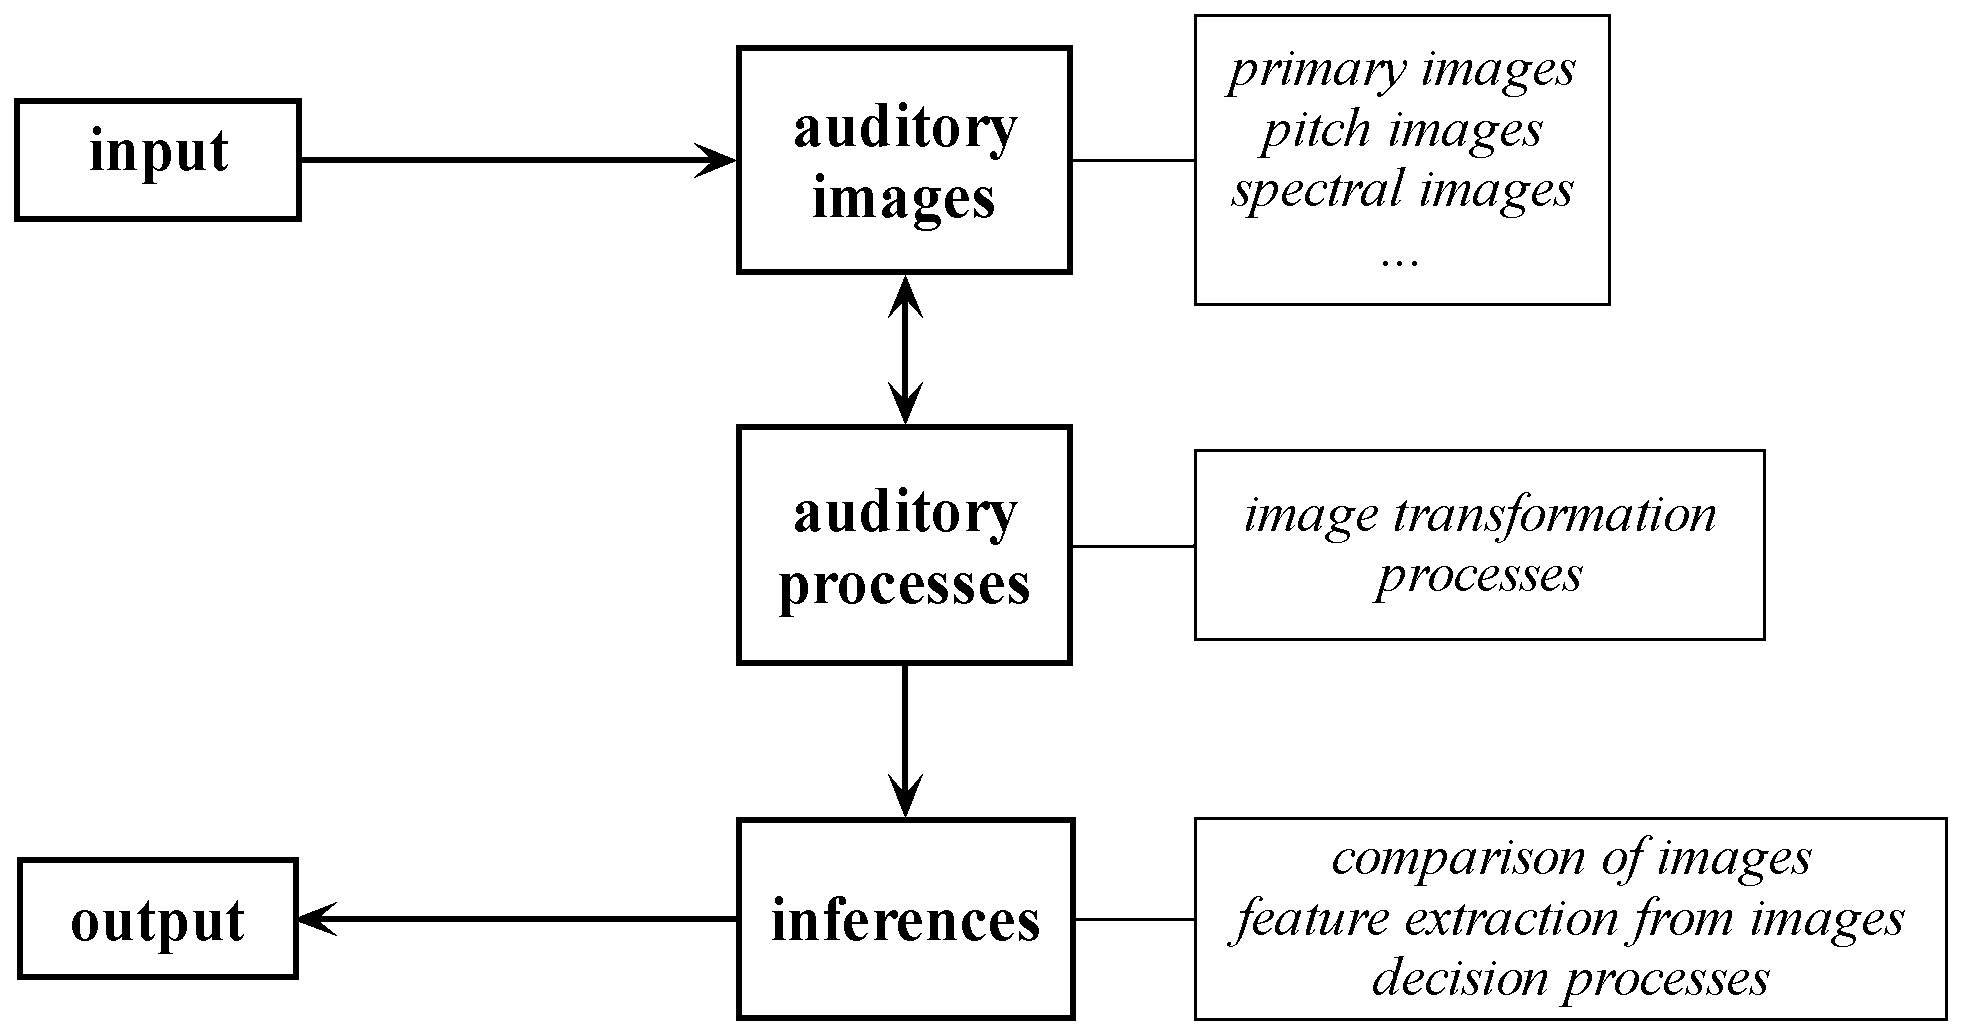
\includegraphics[width=\IPEMDefaultFigureWidth]{Graphics/ConceptualFramework}
    \caption{Overview of the internal representational framework.}
    \label{Fig:ConceptualFramework}
\end{figure}


\newpage
% --------------------------------------------------------------------------------
% Concepts: Modules
% --------------------------------------------------------------------------------

% ================================================================================
\chapter{Modules}
% ================================================================================

% --------------------------------------------------------------------------------
\section{Introduction}
% --------------------------------------------------------------------------------

This chapter describes the modules in the toolbox. A \emph{module}
represents a well-defined process leading to images and (possibly)
an inference. \emph{Well-defined} here means that it corresponds
to a relevant musical perceptual phenomenon. Figure
\ref{Fig:ImageTransformationModules} gives an overview of what we
have in mind as a global picture.

\begin{figure}[h]
    \centering
    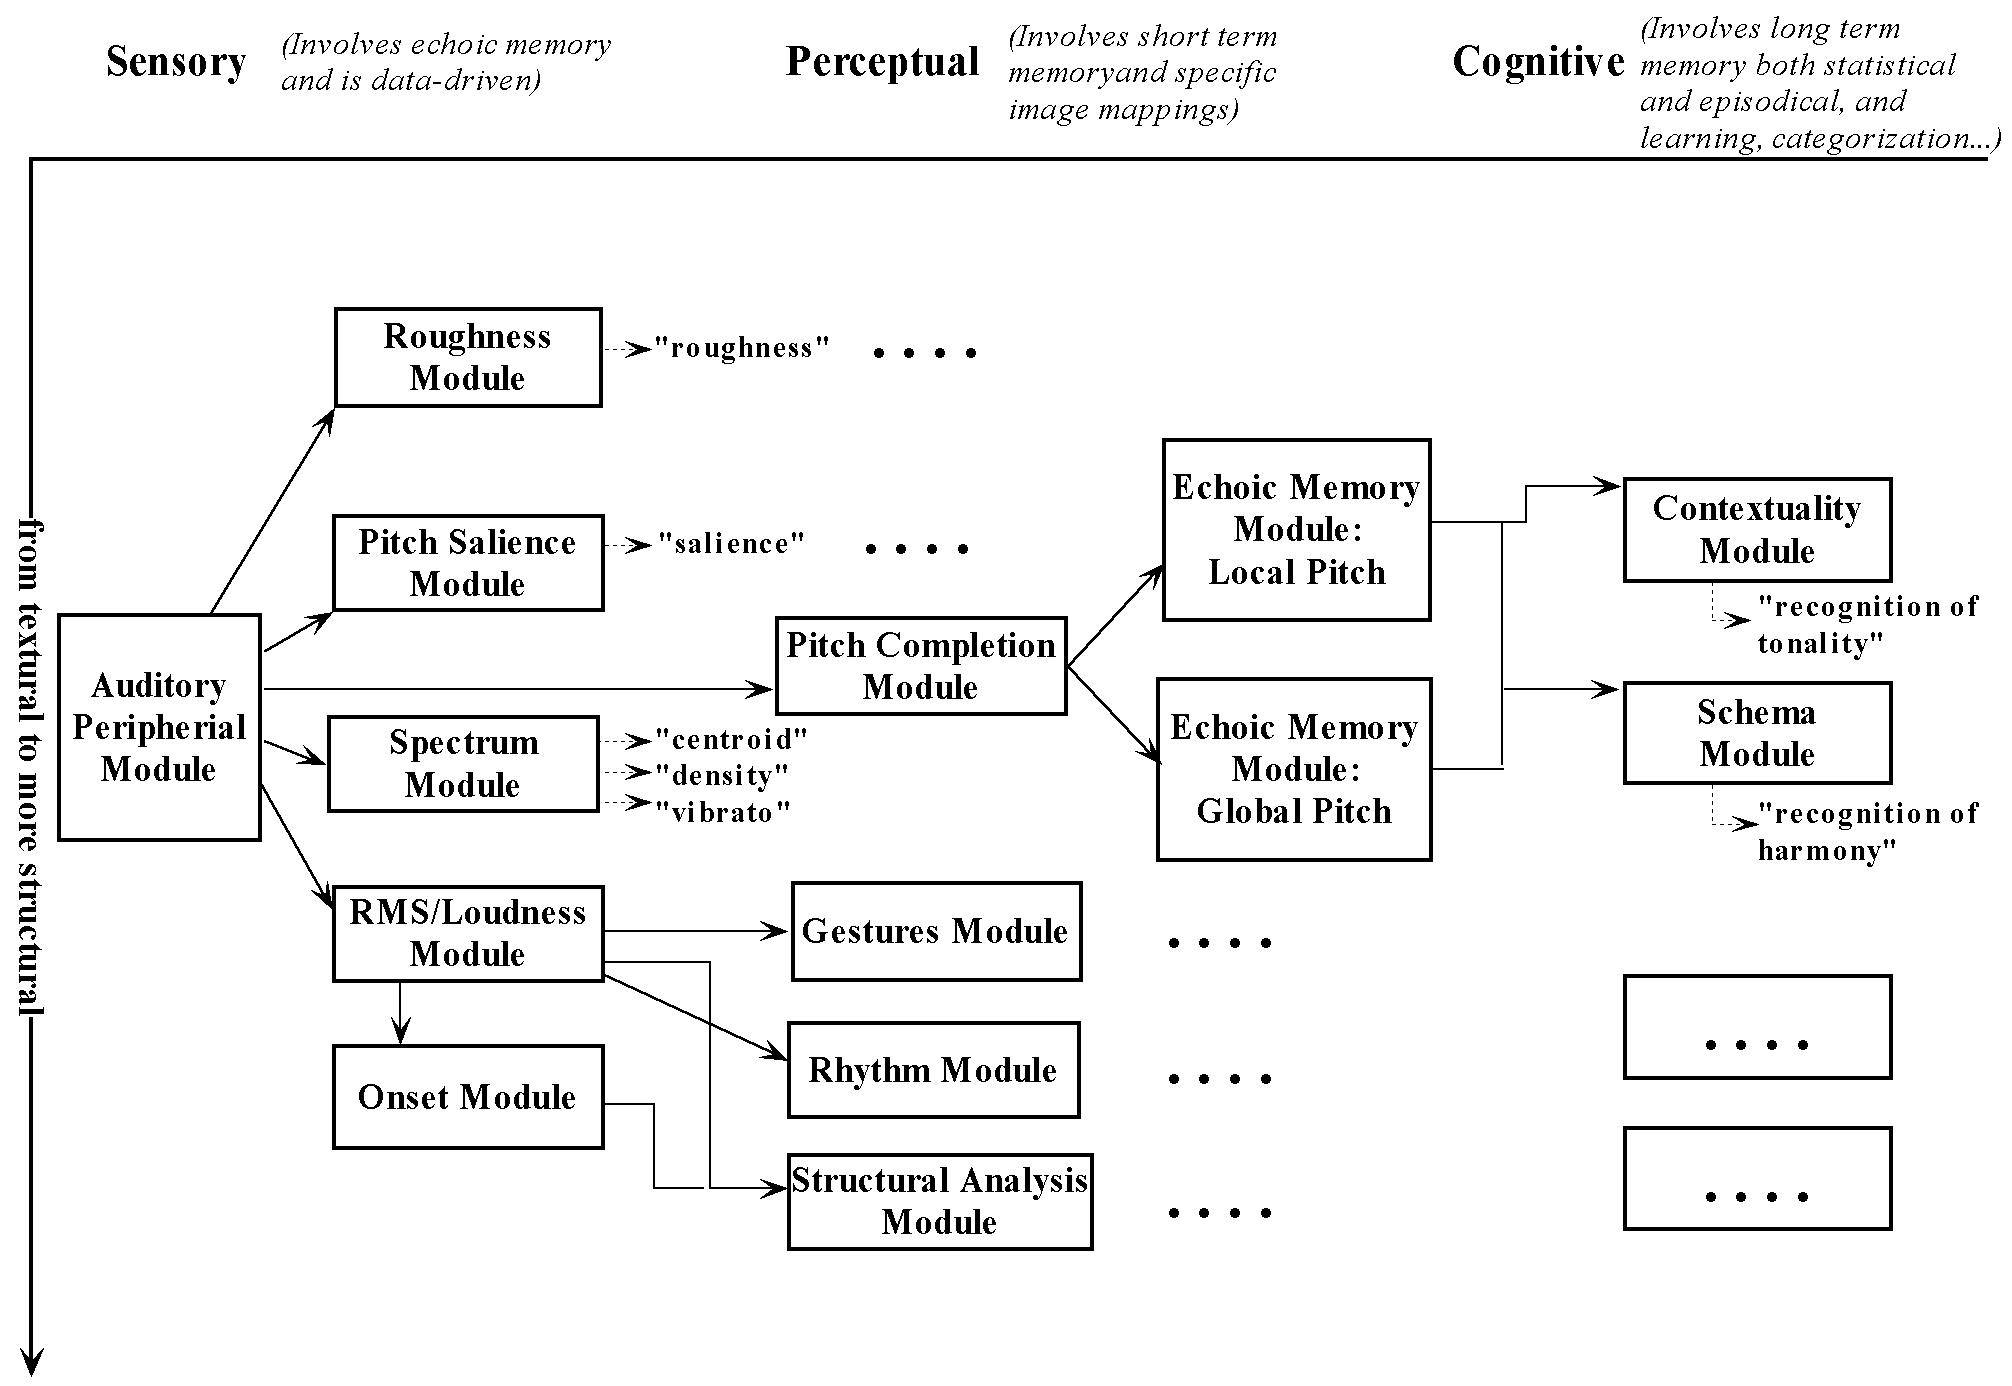
\includegraphics[width=\textwidth]{Graphics/ImageTransformationModules}
    \caption{Chart of image transformation modules, organized
    according to the distinction between sensory, perceptual, and
    cognitive information processing (horizontal axis), and from
    textural to structural (vertical axis). The chart is not
    exhaustive.}
    \label{Fig:ImageTransformationModules}
\end{figure}

The modules on the left are sensory based, the ones on the right
are cognition based and the ones in the middle are perception
based.
\begin{itemize}
    \item Sensory modules involve immediate memory and are based
    on stimulus-driven processing. We assume that they are located
    in the periphery of the auditory system.
    \item Perception modules involve short-term memory and
    specific image mapping from the temporal domain into the
    spatial domain. We assume that they are located in the brain
    stem.
    \item Cognitive modules involve long-term memory, learning and
    categorization. We assume that they are located in the cortex.
\end{itemize}
The modules are furthermore organized from texture (top) to
structure (bottom). This is obviously a simplification but one
that according to our feeling makes sense, at least to some
extent. You should be aware of the fact that this is just one
possible way to visualize the modules and that other
visualizations of the global picture are possible. Notice one more
feature of this chart, in particular the expressions between
quotes, such as "roughness". These labels refer to inferences
associated with the modules. In figure
\ref{Fig:ModulesHighlighted} the modules in the toolbox are
highlighted.

\begin{figure}[h]
    \centering
    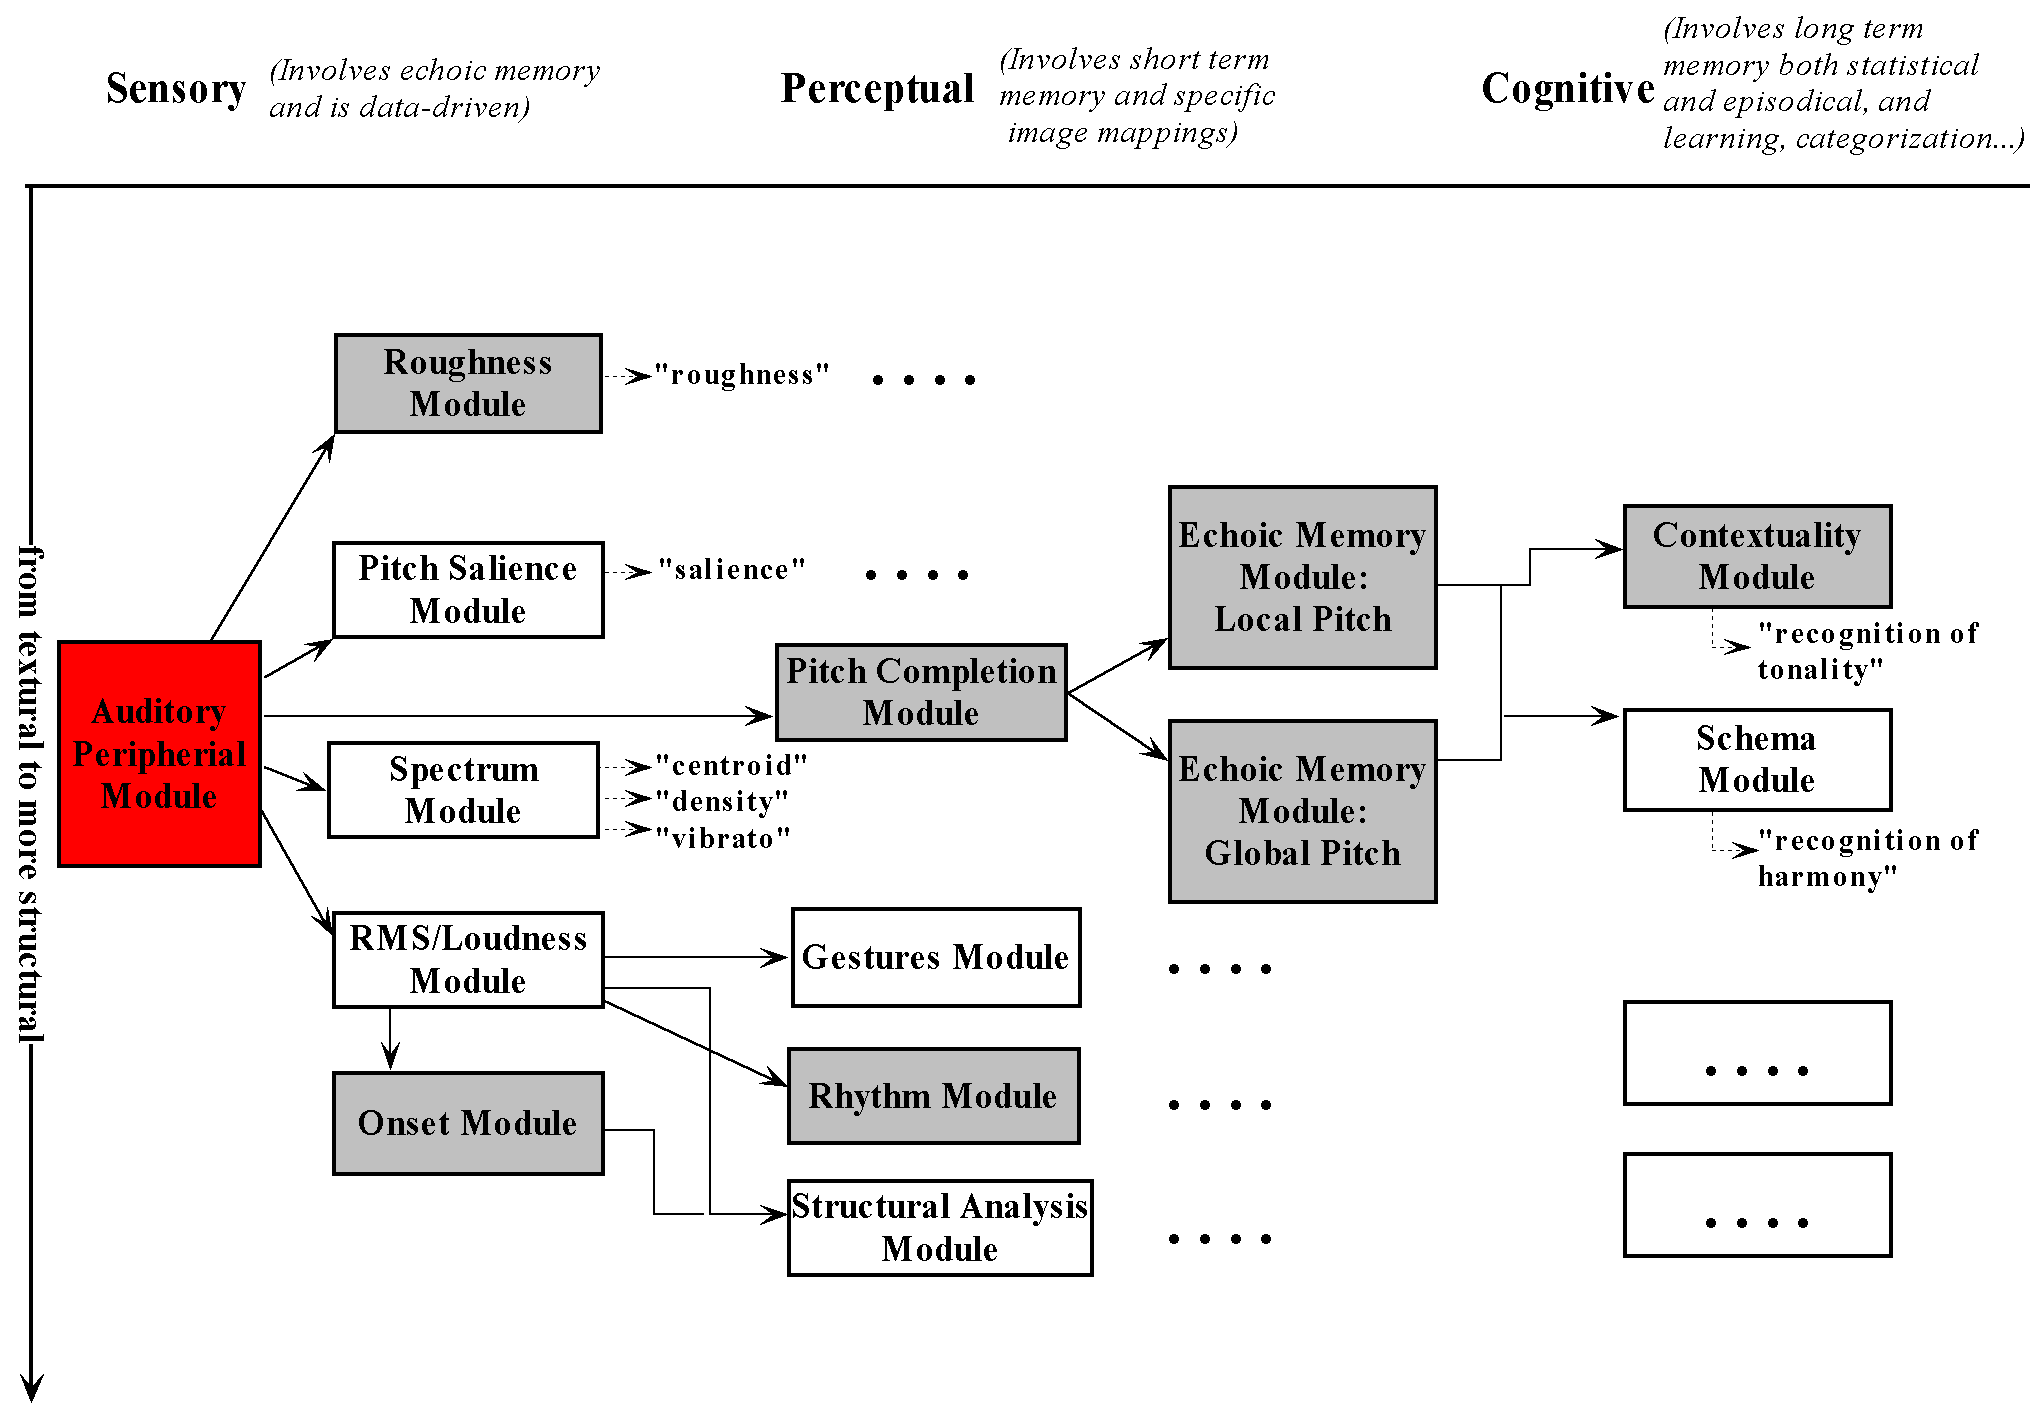
\includegraphics[width=\textwidth]{Graphics/ModulesHighlighted}
    \caption{Situation of the toolbox modules in the global conception}
    \label{Fig:ModulesHighlighted}
\end{figure}

Recall that a module is a well-defined process but that it may
consist of one or more toolbox functions. We learn you how to use
these functions while exploring the modules. If it is the first
time that you read this introduction you can skip the
functional-logical and signal processing descriptions and limit
yourself to the introductory description and the examples. This
should provide enough information to acquire an idea of what the
module is doing.

% --------------------------------------------------------------------------------
% --------------------------------------------------------------------------------
\newpage
\section{Auditory Peripheral Module}
% --------------------------------------------------------------------------------

% Make general target
\hypertarget{Concepts:AuditoryPeripheralModule}{}

% Make target for following functions:
\hypertarget{Concepts:IPEMCalcANI}{}
\hypertarget{Concepts:IPEMCalcANIFromFile}{}
\hypertarget{Concepts:IPEMLoadANI}{}
\hypertarget{Concepts:IPEMSaveANI}{}

\subsection{Introductory description}
% --------------------------------------------------------------------------------

The Auditory Peripheral Module (APM) (fig. \ref{Fig:ModulesAPM})
takes as input a sound and gives as output the \emph{auditory
primary image} which is a kind of physiological justified
representation of the auditory information stream along the VIIIth
cranial nerve. The musical signal is decomposed in different
subbands and represented as neural patterns. The patterns are
rate-codes, which means that they provide the probability of
neuronal firing during a short interval of time.
\begin{figure}[h]
    \centering
    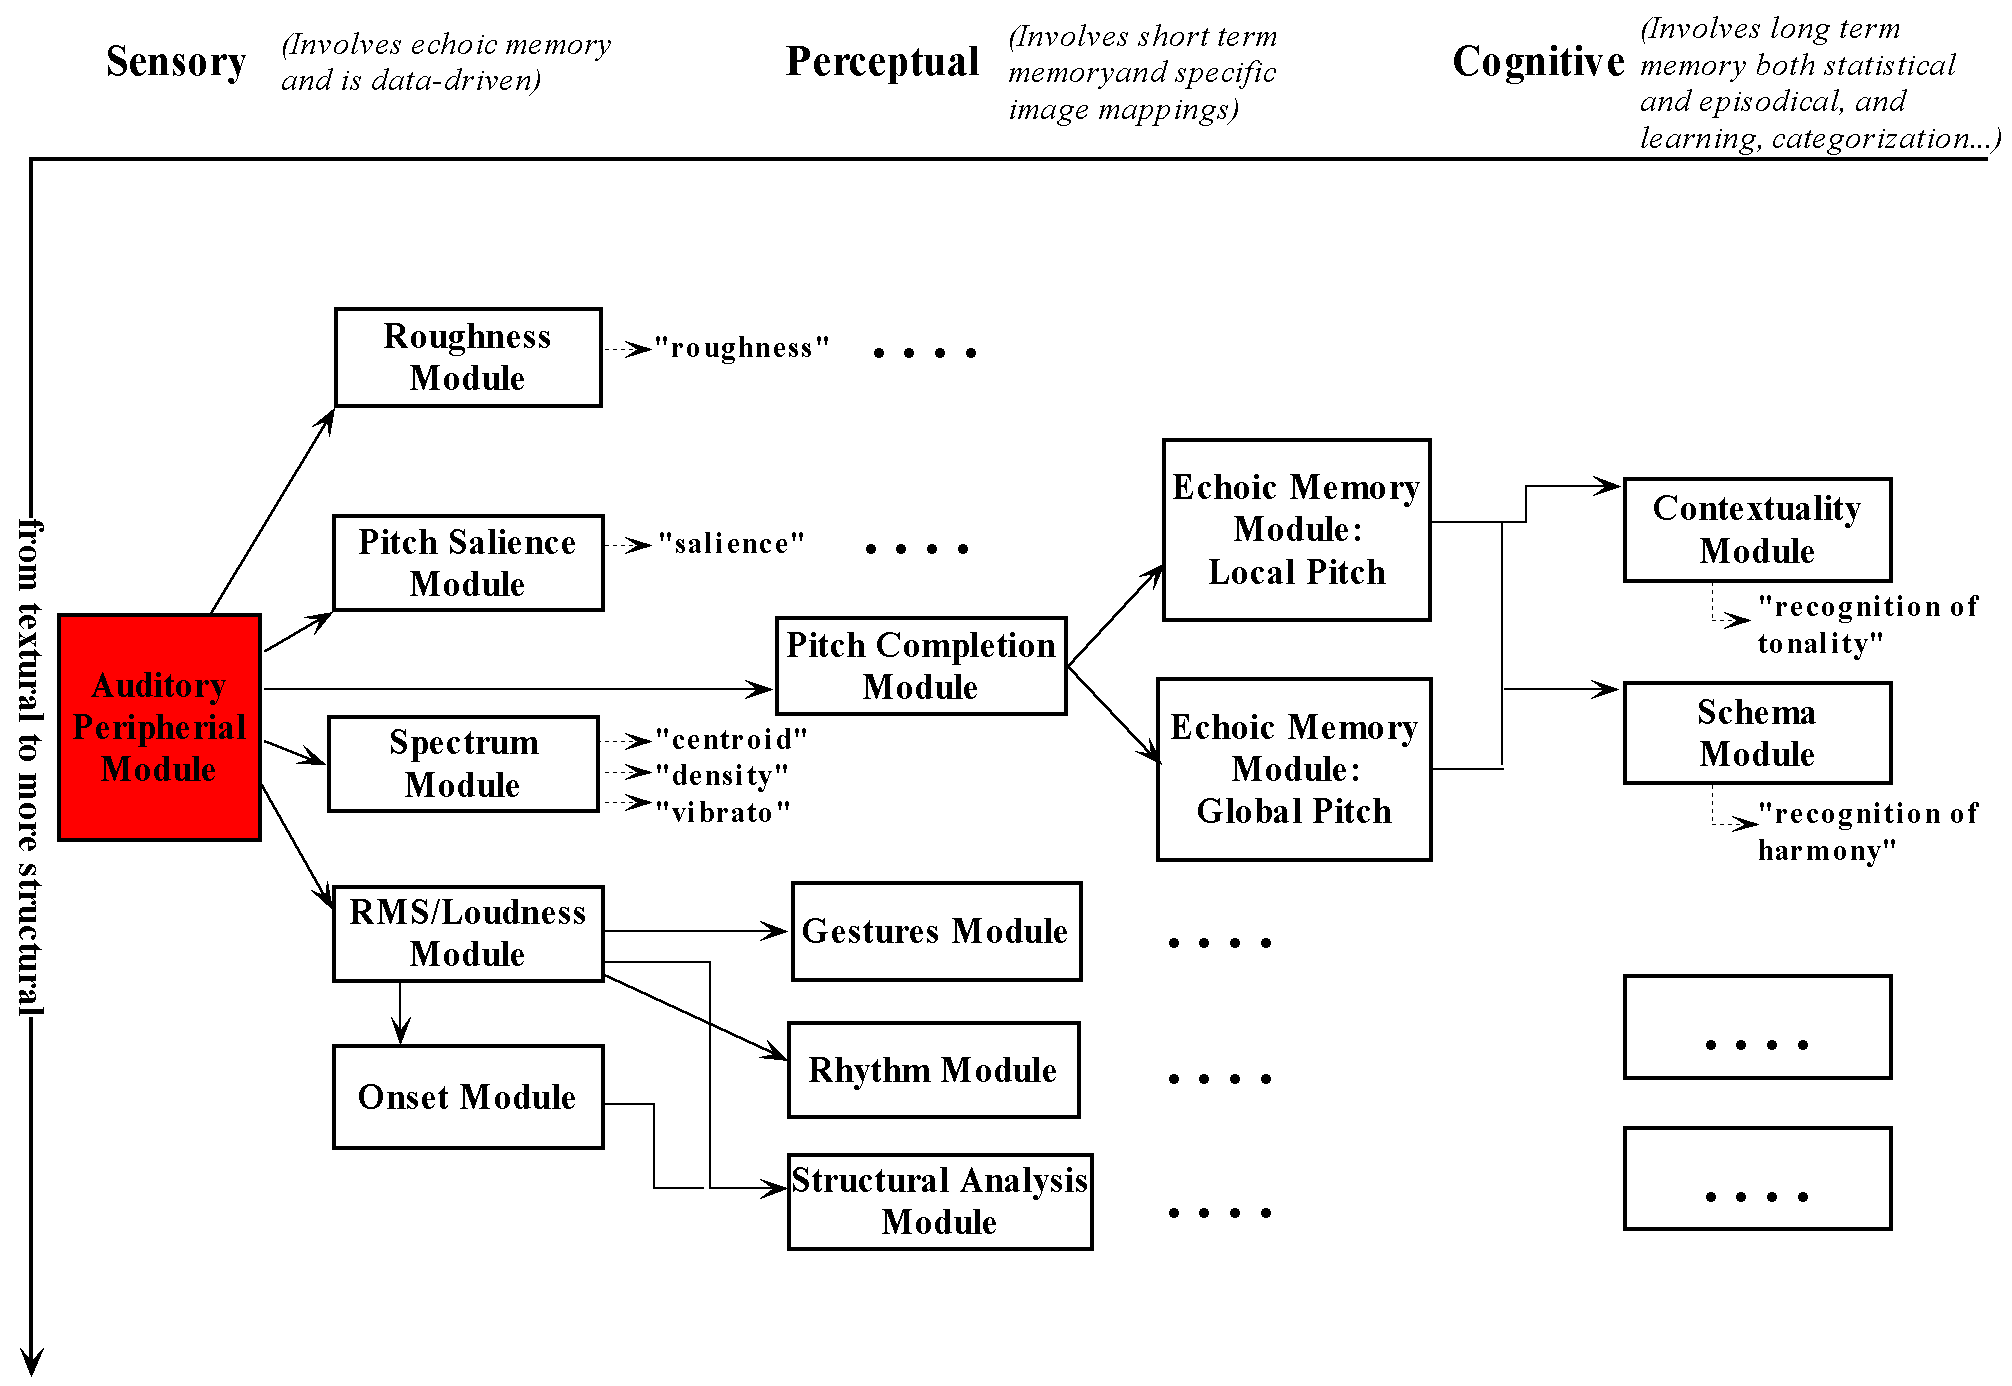
\includegraphics[width=\textwidth]{Graphics/ModulesAPM}
    \caption{Chart of image transformation modules, with APM highlighted}
    \label{Fig:ModulesAPM}
\end{figure}

The Auditory Peripheral Module that we use is an adapted version
of \citeA{VanImmerseelMartens:92} model of the auditory periphery.
The processing stages involve:
\begin{itemize}
\item
    Simulation of the filtering of the outer and middle ear.
\item
    Simulation of basilar membrane resonance in the inner ear. This is
    implemented by an array of band-pass filters whose center
    frequencies are spaced on a critical band scale (Bark scale).
    The bandwidth of each filter equals
    a critical band.
\item
    Simulation of a hair cell model. This converts the band-pass filtered signals into
    neural {\sl rate-code} patterns. This operation deals with half-wave rectification and
    dynamic range compression.
\end{itemize}

Figure \ref{Fig:APMModule} gives a view of the transformation of
sound into primary images.
\begin{figure}[h]
    \centering
    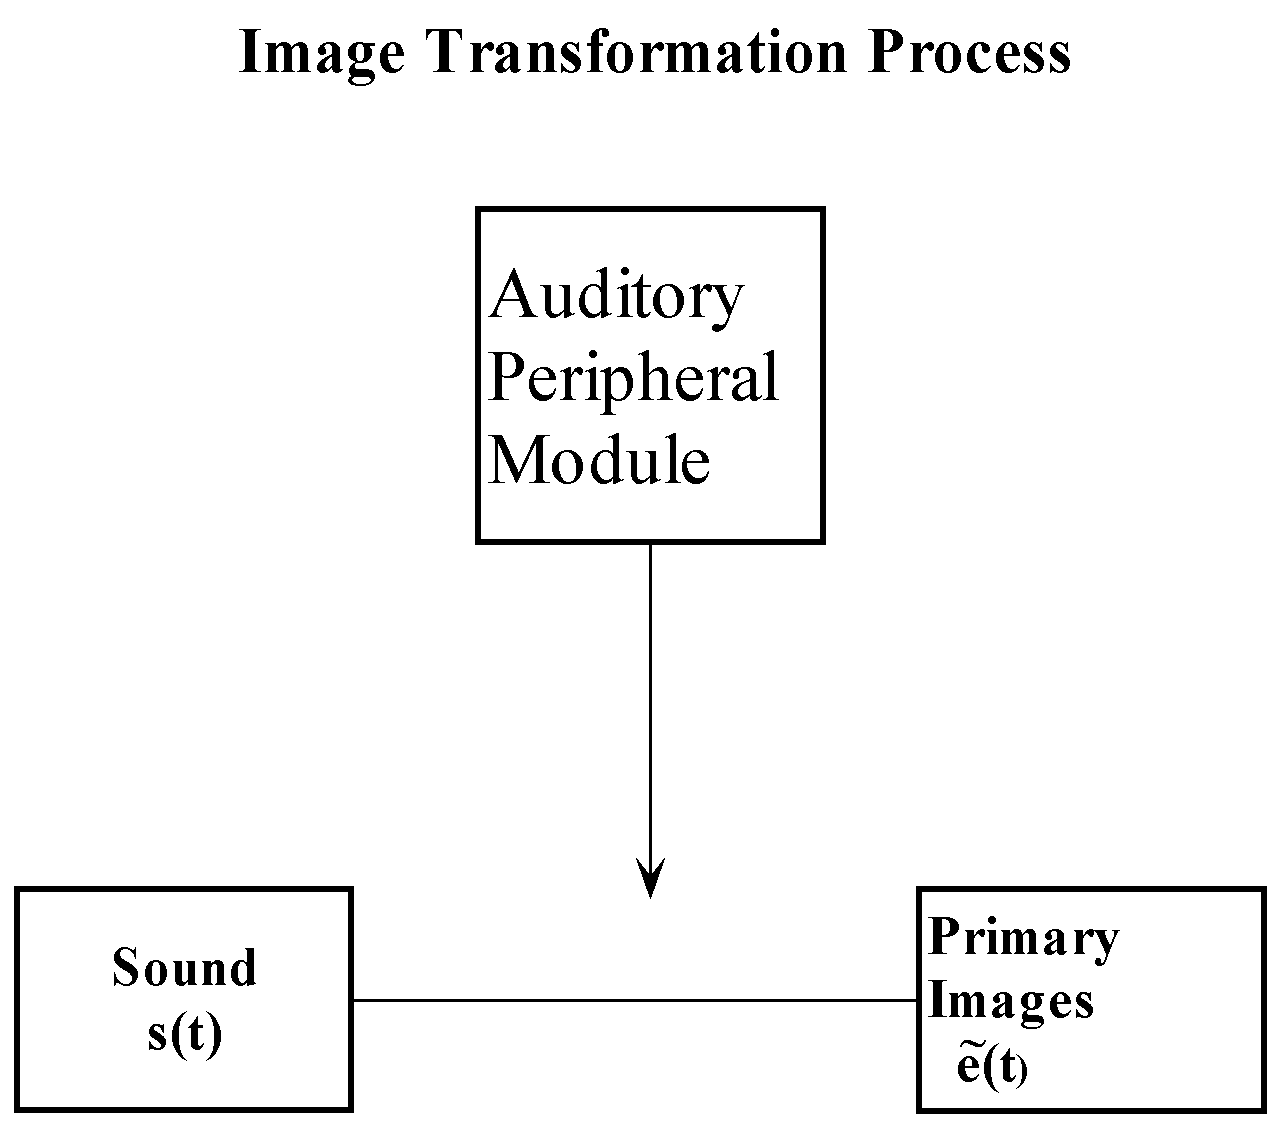
\includegraphics[width=\IPEMDefaultFigureWidth]{Graphics/APMModule}
    \caption{Image Transformation Process: Auditory Peripheral  Module}
    \label{Fig:APMModule}
\end{figure}

\subsection{Functional-logical description}
% --------------------------------------------------------------------------------

The APM can be described as a function which transforms a musical
sound signal $s(t)$ into a set of patterns $e_n(t)$ (with $n = 1,
2, ..., C$) that encode the responses of auditory neuronal fibers
spread along the basilar membrane (see Equation \ref{Eq1}). The
auditory filters, sometimes also called {\sl channels}, simulate
the neuronal band-pass characteristics and the firing rate
encoding. The frequency range covered by the auditory filters
depends on the center frequencies of the filters, the number of
chosen channels and the chosen distance between the channels. In
most of our simulations we chose forty channels ($C=40$), half a
critical band apart from each other. This covers a range from 140
Hz to 8877 Hz. As a short-hand we use the notation:

\begin{displaymath}
APM:~s(t) \rightarrow \left[
\begin{array}{l}
e_1(t) \\ e_2(t) \\ \cdots \\ e_{C}(t)
\end{array}
\right]=~e(t,c)~=~\tilde{e}(t)
\end{displaymath}
or, alternatively,
\begin{equation}
APM:~s(t) \rightarrow \tilde{e}(t) \label{Eq1}
\end{equation}

The pattern denoted $\tilde{e}(t)$ is called the \emph{primary
image} or \emph{auditory nerve image (ANI)} of $s(t)$. It should
be considered the auditory counterpart of D.~Marr's {\sl primal
sketch} in the domain of visual perception \cite{Marr:82}. The
tilde character here denotes a vector in which each
vector-component corresponds to one auditory filter. The arrow
represents a causal transformation, in this case from a sound into
the auditory nerve image.

In our terminology, a \emph{running vector} means that the values
of the vector-components change over time, where $t$ denotes time.
The pattern $\tilde{e}(t)$ thus represents the neural activation
in all subbands over subsequent time steps. The notation $e(t,c)$
means the same, whereas $e(t,c)$ for fixed $c$ is the neural
activation in one particular channel $c$.

\subsection{Signal processing description}
% --------------------------------------------------------------------------------
For a full description of this module we refer to
\citeA{VanImmerseelMartens:92}. We limit ourselves to a more technical
verbal summary.

The auditory peripheral module simulates the cochlear mechanical
filtering using an array of overlapping band-pass filters.
%The
%module provides rate-code patterns of neural discharge at the
%level of the auditory nerve, representing the amount of neural
%excitation during short time intervals.
The basic steps of this model, shown in figure
\ref{Fig:AuditoryModel} can be summarized as follows.

\begin{figure}[h]
    \centering
    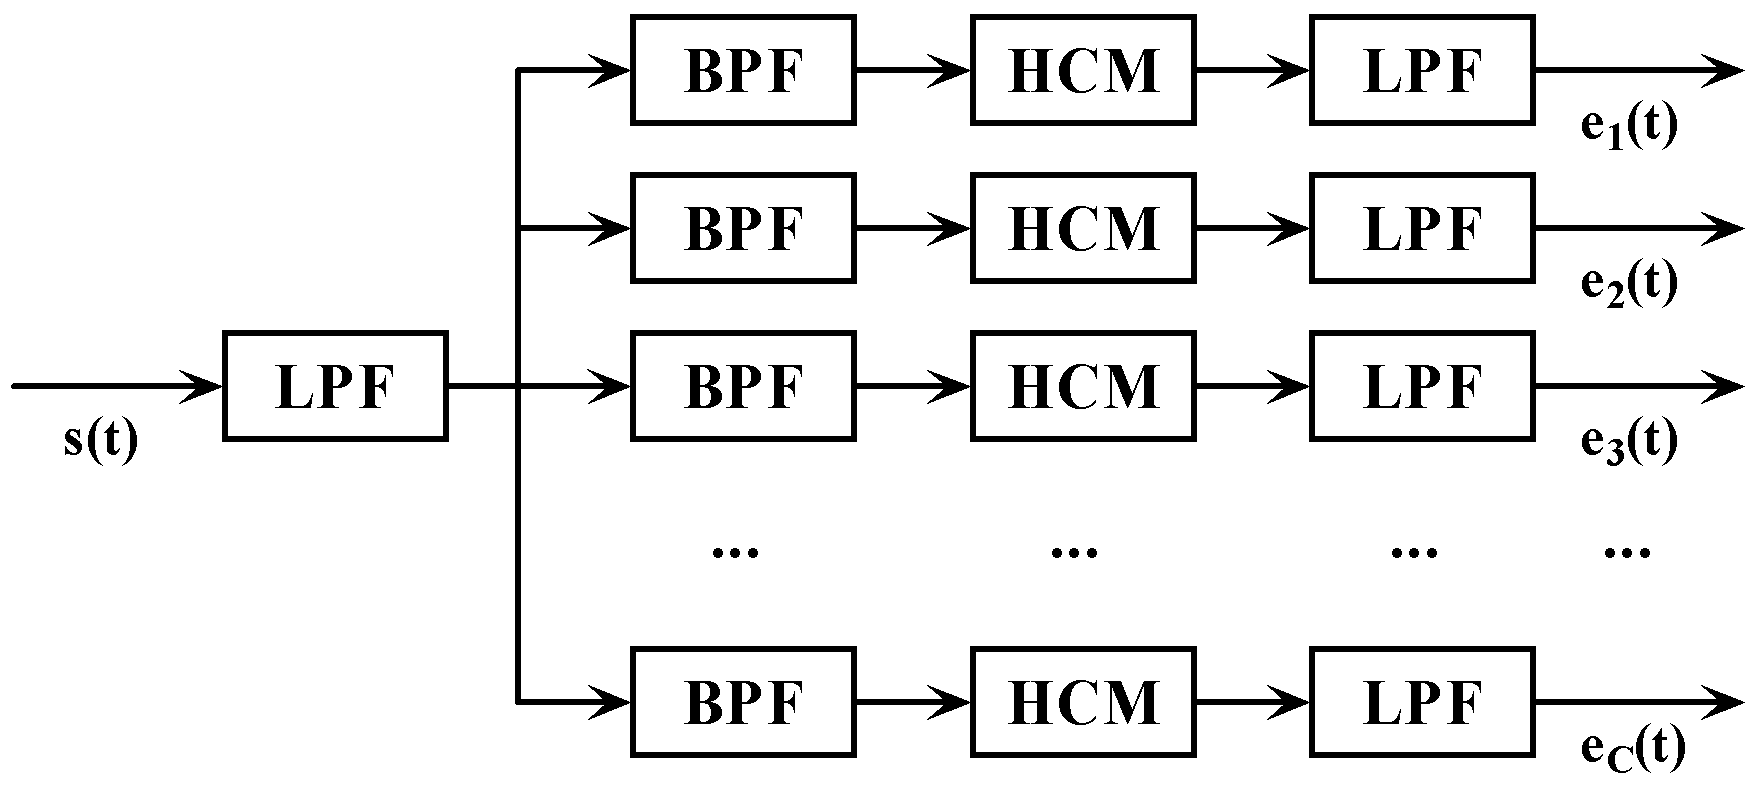
\includegraphics[width=\IPEMDefaultFigureWidth]{Graphics/AuditoryModel}
    \caption{Schema of the Auditory Peripheral Module. }
    \label{Fig:AuditoryModel}
\end{figure}

\begin{itemize}
\item
    The outer and inner ear filtering is implemented as a
    second-order low-pass filter (LPF) with a resonance frequency of
    4 kHz. This accounts for the overall frequency response of the
    ear, a coarse approximation to the Fletcher-Munson curves.
\item
    The filtering in the cochlea is implemented by an array of
    band-pass filters (BPF). In many of the simulations in this book,
    we use center frequencies that are spaced equidistantly on a
    critical band scale, having an overlap of half a critical band.
    Forty channels are used with center frequencies ranging from 141
    to 8877 Hz. The filters have a 3 dB bandwidth of one critical
    band; a low-frequency slope of about 10 dB per critical band unit
    and a high-frequency slope of about 20 dB per critical band unit.
\item
    The mechanical to neural transduction is performed by a hair cell
    model (HCM), which is assumed identical in all channels. The HCM
    is a forward-driven gain controlled amplifier that incorporates
    half-wave rectification and dynamic range compression. The HCM
    introduces distortion products that reinforce the low frequencies
    that correspond to the frequency of the beats.
\item
    A low-pass filter at 1250 Hz does an envelope extraction of the
    patterns in each channel. This low-pass filter accommodates for
    the loss of synchronization observed in the primary auditory
    nerve. The filter can be argued to have an effect on the width of
    the critical band for high $f_c$ although these may fall out of
    the scope of most musically relevant tones
    \cite{GreenwoodJoris:1996}.
\end{itemize}

The output $e(t,c)$ for fixed $c$ represents the rate-code of
neural discharge in channel $c$. This pattern is also called the
\emph{auditory nerve pattern} in channel $c$.

\subsection{Implementation}
% --------------------------------------------------------------------------------

\begin{tabularx}{\linewidth}{llX}
\hyperlink{FuncRef:IPEMCalcANI}{IPEMCalcANI} & - & Calculates auditory nerve image from signal\\
\hyperlink{FuncRef:IPEMCalcANIFromFile}{IPEMCalcANIFromFile} & - & Calculates auditory nerve image directly from sound file\\
\hyperlink{FuncRef:IPEMLoadANI}{IPEMLoadANI} & - & Loads auditory nerve image from .mat file\\
\hyperlink{FuncRef:IPEMSaveANI}{IPEMSaveANI} & - & Saves auditory nerve image to .mat file\\
\end{tabularx}

\subsection{Examples}
% --------------------------------------------------------------------------------

In this section we provide some examples of how to transform
musical signals into primary images (auditory nerve images). A
straightforward function is
\hyperlink{FuncRef:IPEMCalcANIFromFile}{IPEMCalcANIFromFile} which
allows you to read in a wav-file. If the wav-file
\emph{SchumannKurioseGeschichte.wav} is stored in the "Sounds"
subdirectory of the default input directory (see also the
\hyperlink{ReferenceManual:Installation}{installation}
instructions), and you agree with the default 40 subbands and the
overlap of 1/2 critical band, then the function is simply:\\

\IPEMCodeExtract{IPEMCalcANIFromFile('SchumannKurioseGeschichte.wav',[],[],1);}\\

Similarly, if \emph{ShepardCChord.wav} is stored in that same directory, you can write:\\

\IPEMCodeExtract{IPEMCalcANIFromFile('ShepardCChord.wav');}\\

The results should be similar to what you see on these pages
(except the score, of course):
\begin{enumerate}
\item
    Figure \ref{Fig:SchumannScore} shows the score of the
    \IPEMSound{Sounds/SchumannKurioseGeschichte.wav}{used
    excerpt of Schumann's Kuriose Geschichte}.
    \footnote{Robert Schumann "Kinderszenen-Kreisleriana", played
    by Martha Argerich (Deutsche Grammophon 410 653-2, 1984)}
\item
    Figure \ref{Fig:SchumannANIandAudioSignal} shows the results of processing
    this short excerpt with the Auditory Peripheral Module. The upper panel shows
    the waveform, the lower panel shows the primary image.
\item
    Figure \ref{Fig:ShepardCChordANIandAudioSignal} shows the results of processing
    \IPEMSound{Sounds/ShepardCChord.wav}{a signal consisting of
    the C major chord, build up from 3 Shepard tones} with the Auditory Peripheral Module.
    Again, the upper panel shows the waveform, the lower panel shows the primary image.
\end{enumerate}

To generate a Shepard-chord yourself, you can type (see
\hyperlink{FuncRef:IPEMShepardToneComplex}{IPEMShepardToneComplex}):\\

\IPEMCodeExtract{MyShepardChord = IPEMShepardToneComplex([1 0 0 0 1 0 0 1 0 0 0 0],1,22050,1);}\\

Now you generated a signal that is stored in
\IPEMCodeExtract{MyShepardChord}. And you can play it in the usual
MATLAB way with:\\

\IPEMCodeExtract{sound(MyShepardChord,22050);}\\

Pay attention to the fact that \IPEMCodeExtract{MyShepardChord} is
a signal in the MATLAB environment, not a wav-file. To process
this signal with the auditory peripheral module you can do:\\

\IPEMCodeExtract{IPEMCalcANI(MyShepardChord,22050);}\\

Note that the number 22050 is the sampling rate which should be
specified, and \IPEMCodeExtract{MyShepardChord} is a variable in
MATLAB, therefore it should not be between quotes.

\begin{figure}[h]
    \centering
    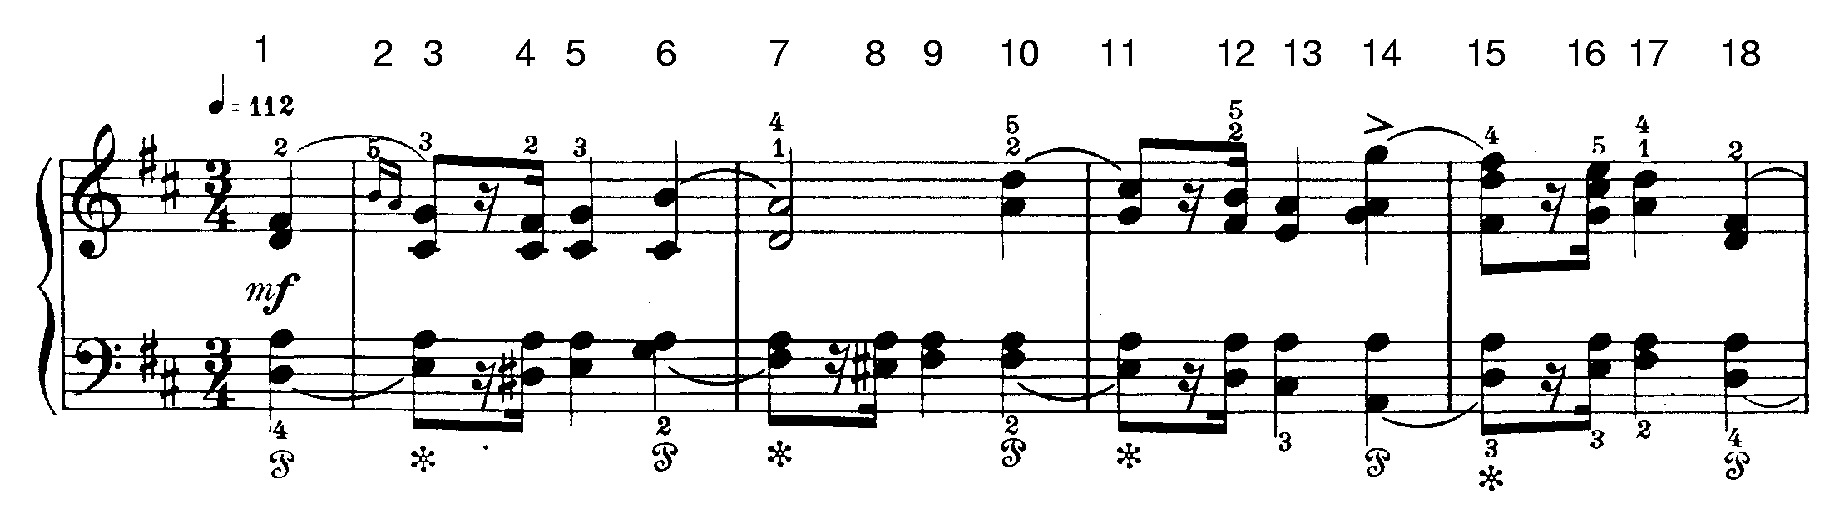
\includegraphics[width=\IPEMDefaultFigureWidth]{Graphics/SchumannScore}
    \caption{The first four measures of Schumann's piece "Kuriose Geschichte"}
    \label{Fig:SchumannScore}
\end{figure}

\begin{figure}[h]
    \centering
    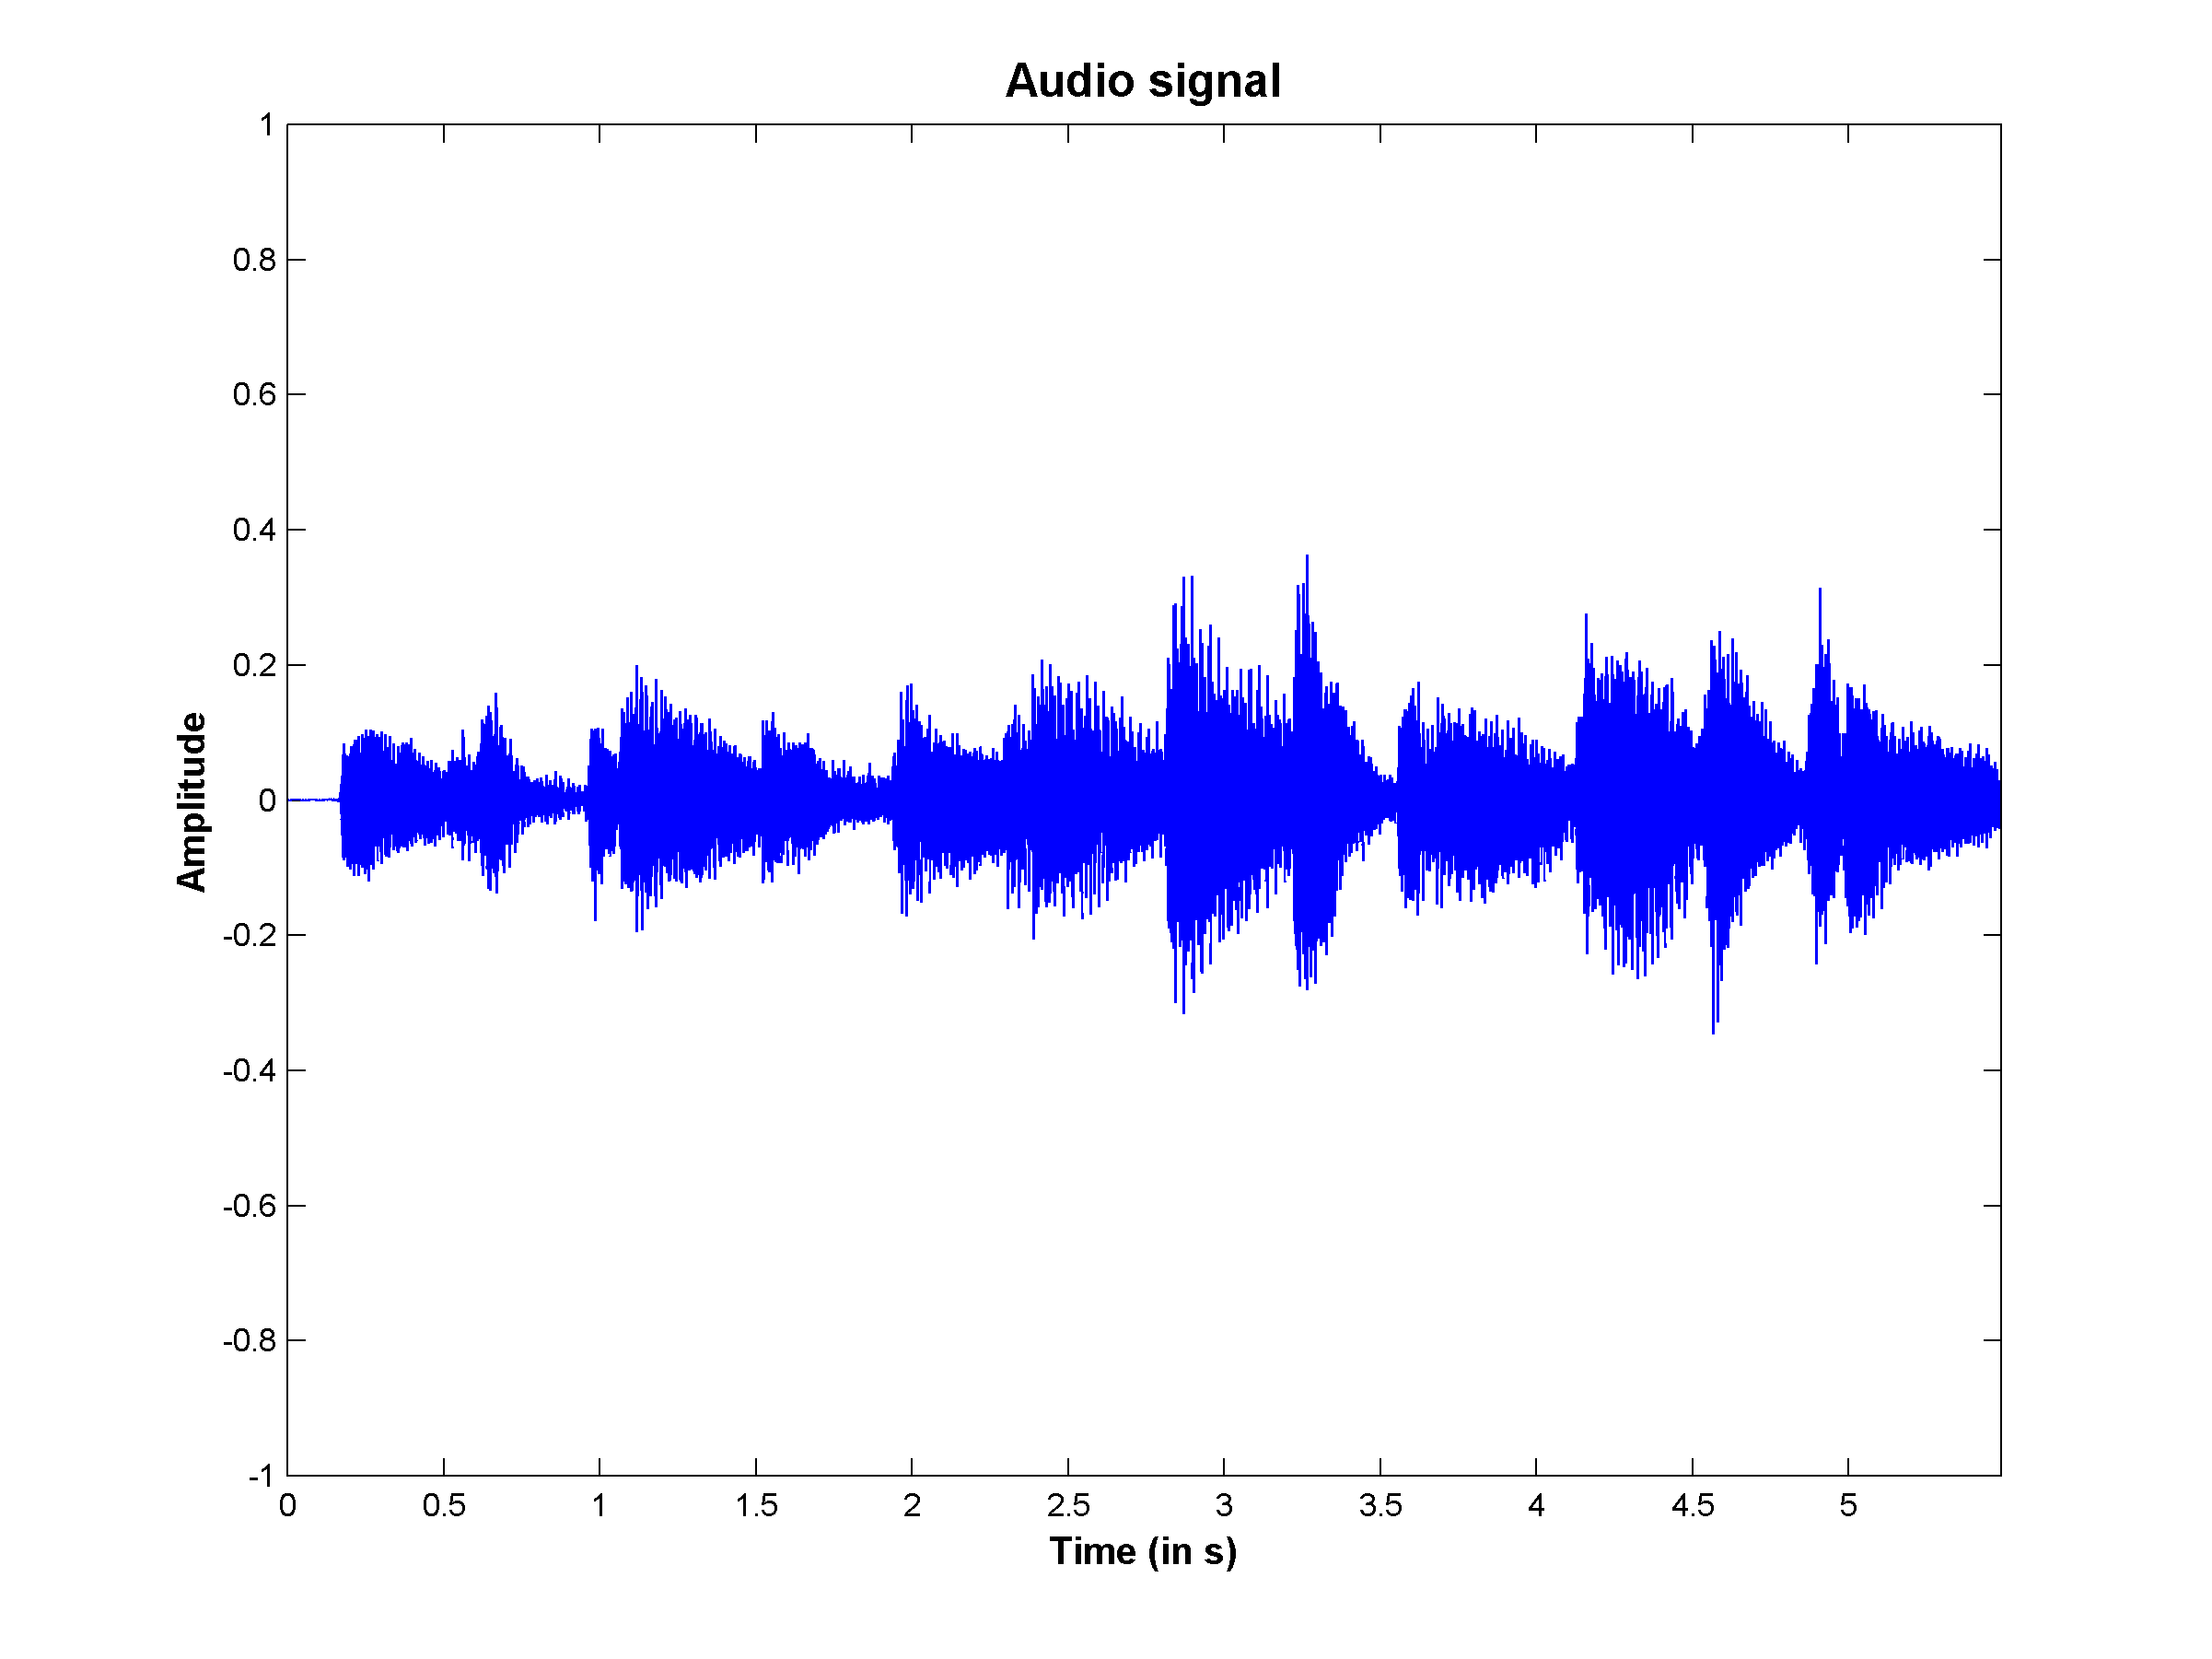
\includegraphics[width=\IPEMDefaultFigureWidth]{Graphics/SchumannAudioSignal}
    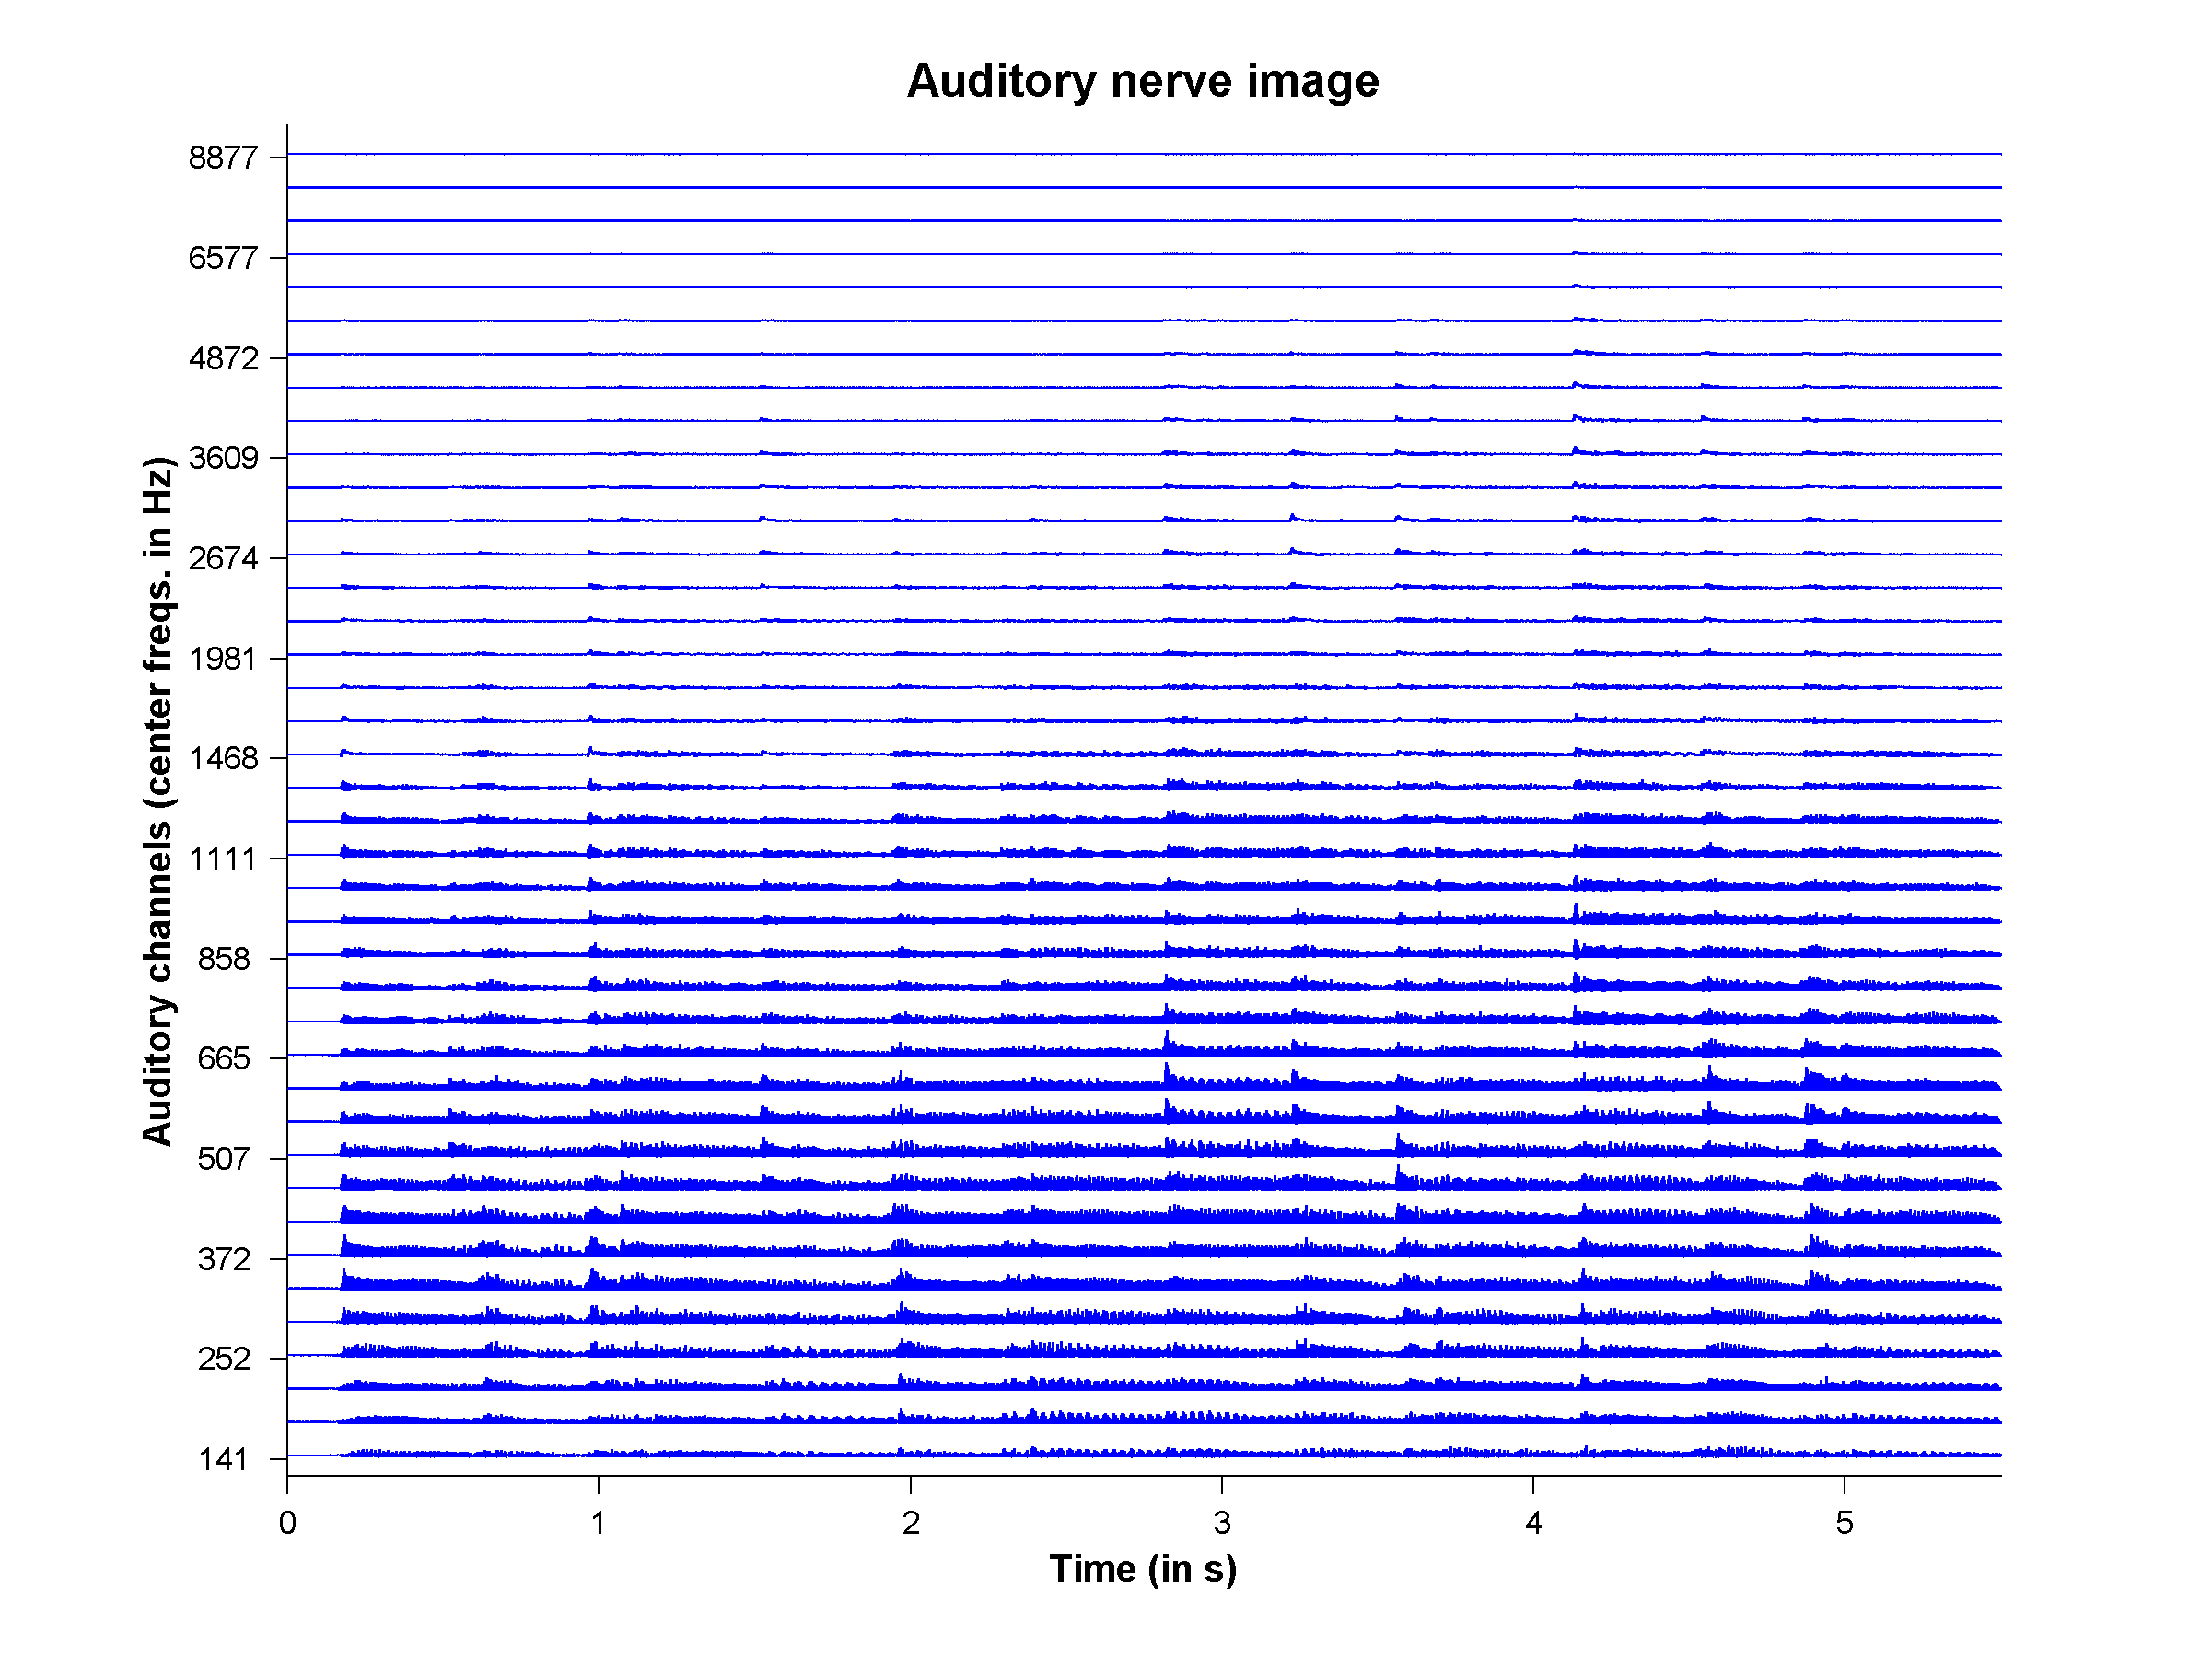
\includegraphics[width=\IPEMDefaultFigureWidth]{Graphics/SchumannANI}
    \caption{Top: waveform of a short excerpt of Schumann's Kuriose Geschichte. Bottom: primary image}
    \label{Fig:SchumannANIandAudioSignal}
\end{figure}

\begin{figure}[h]
    \centering
    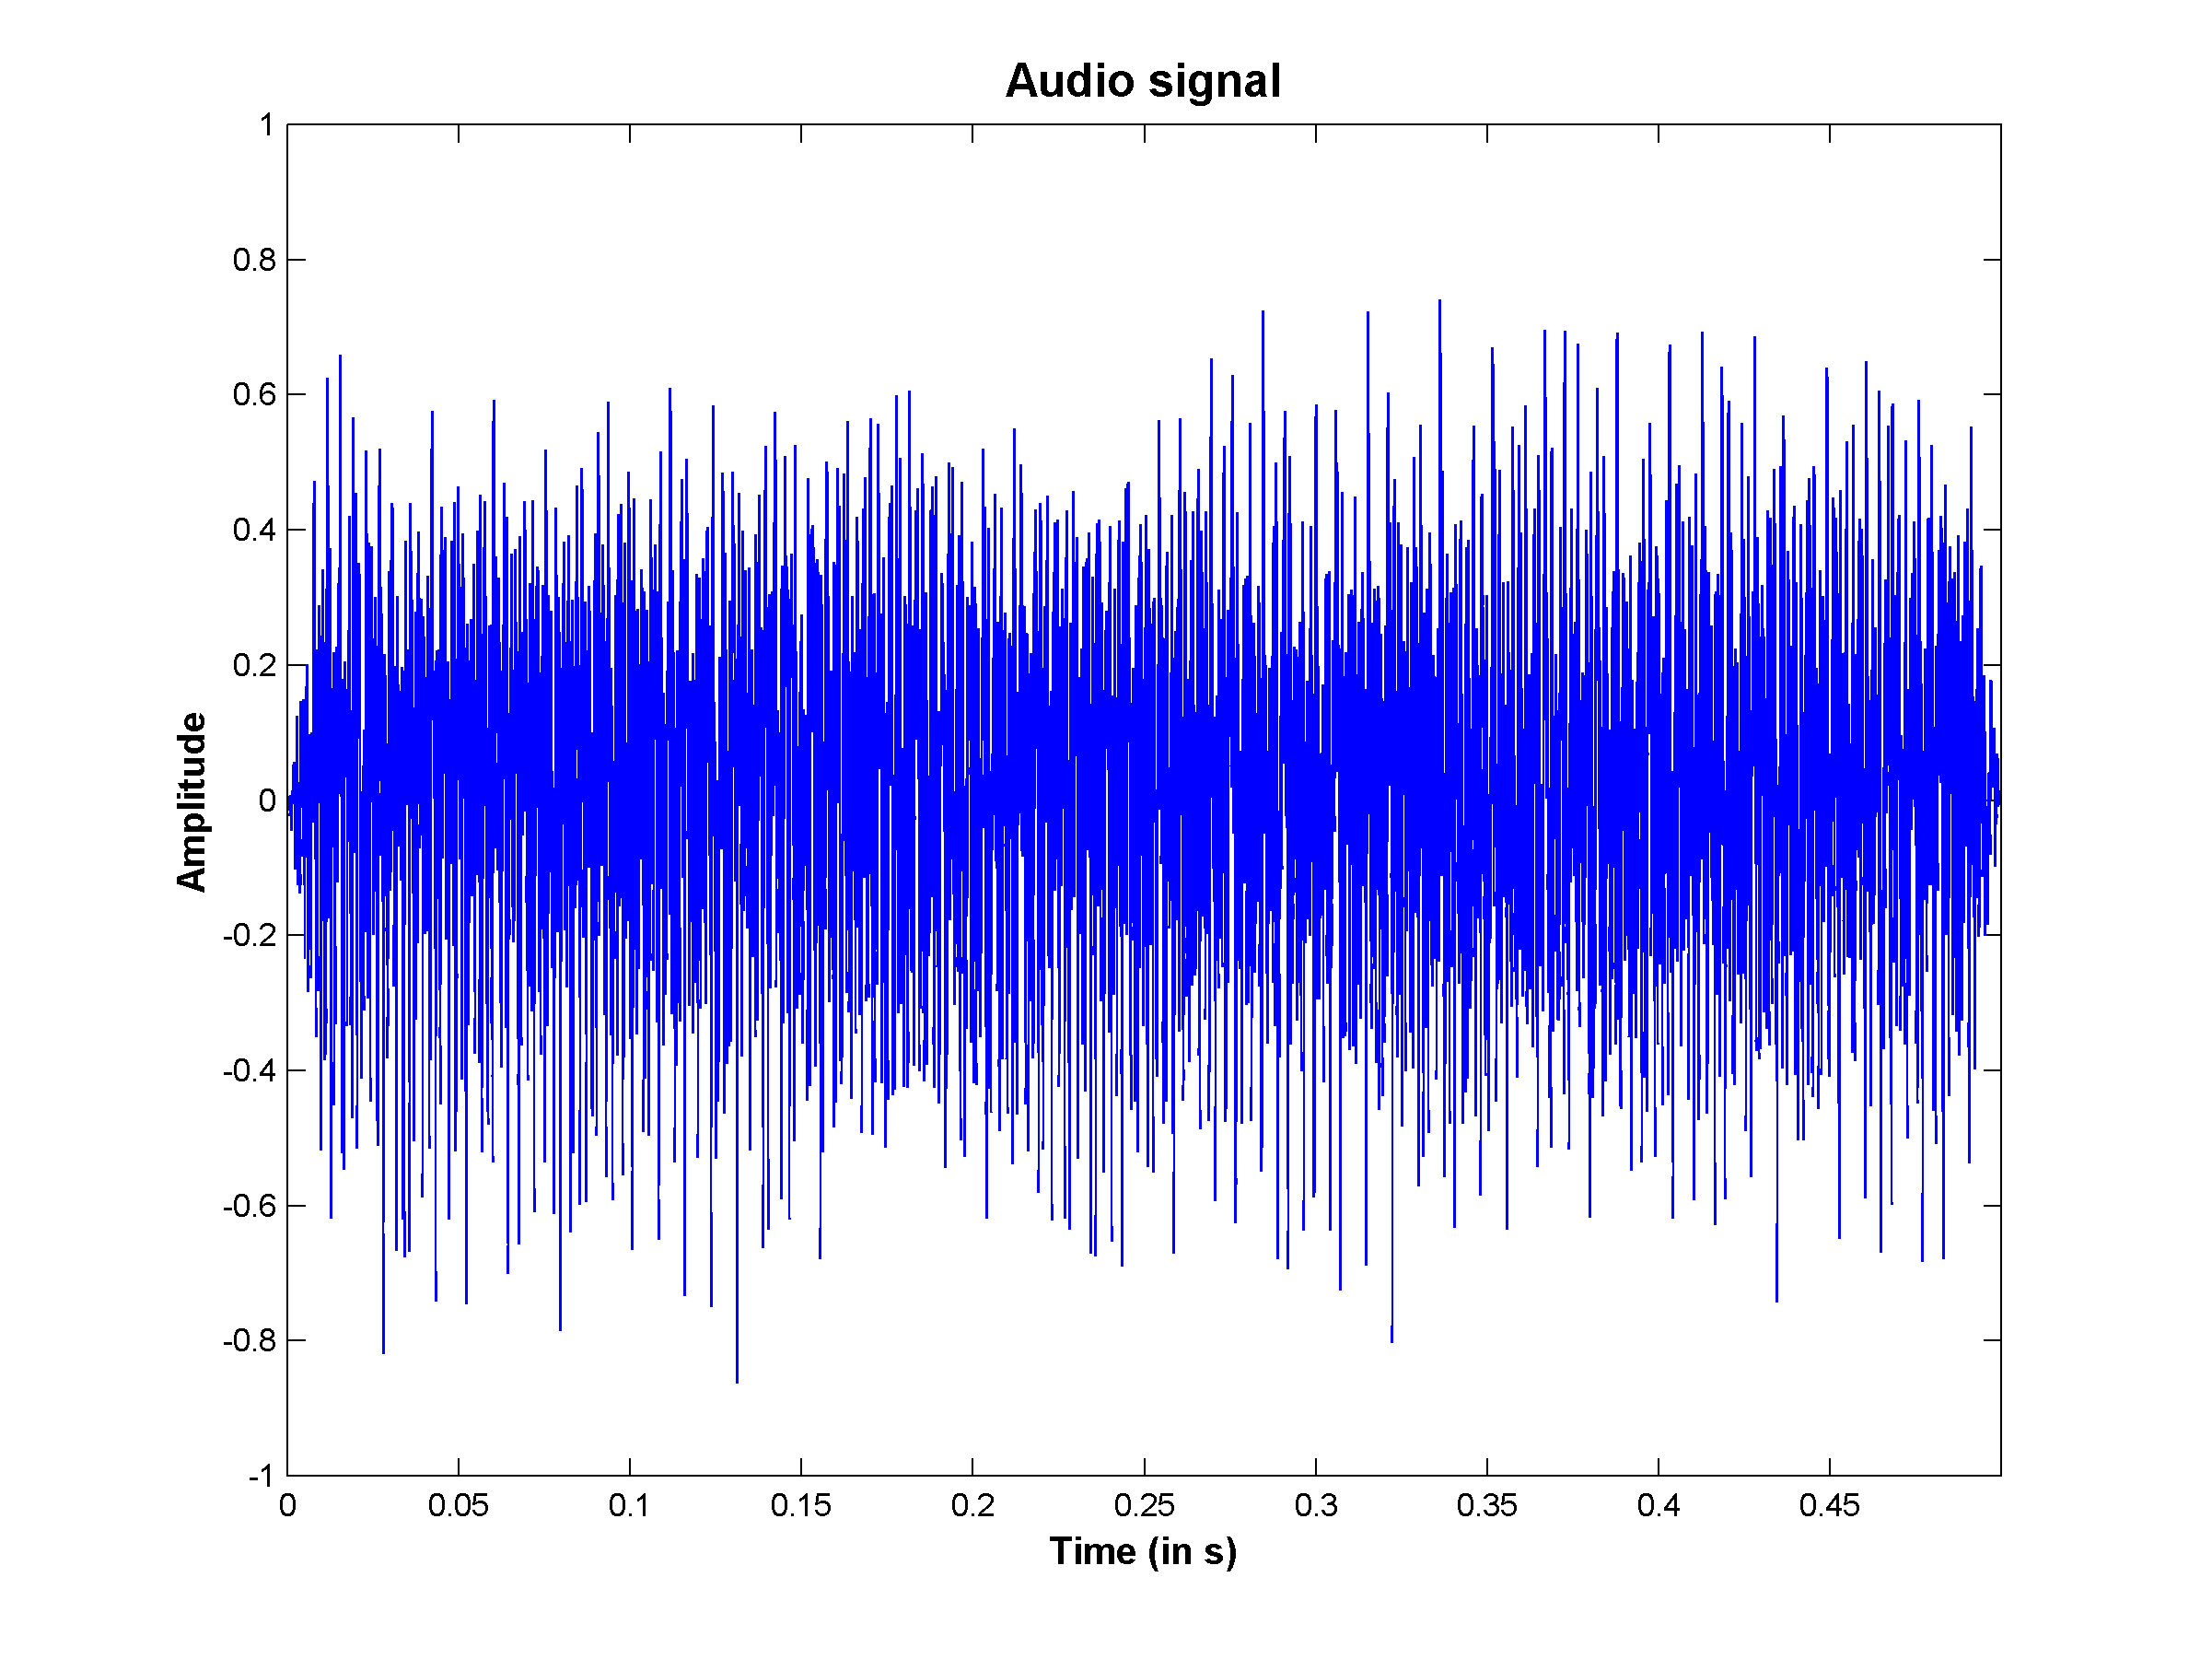
\includegraphics[width=\IPEMDefaultFigureWidth]{Graphics/ShepardCChordAudioSignal}
    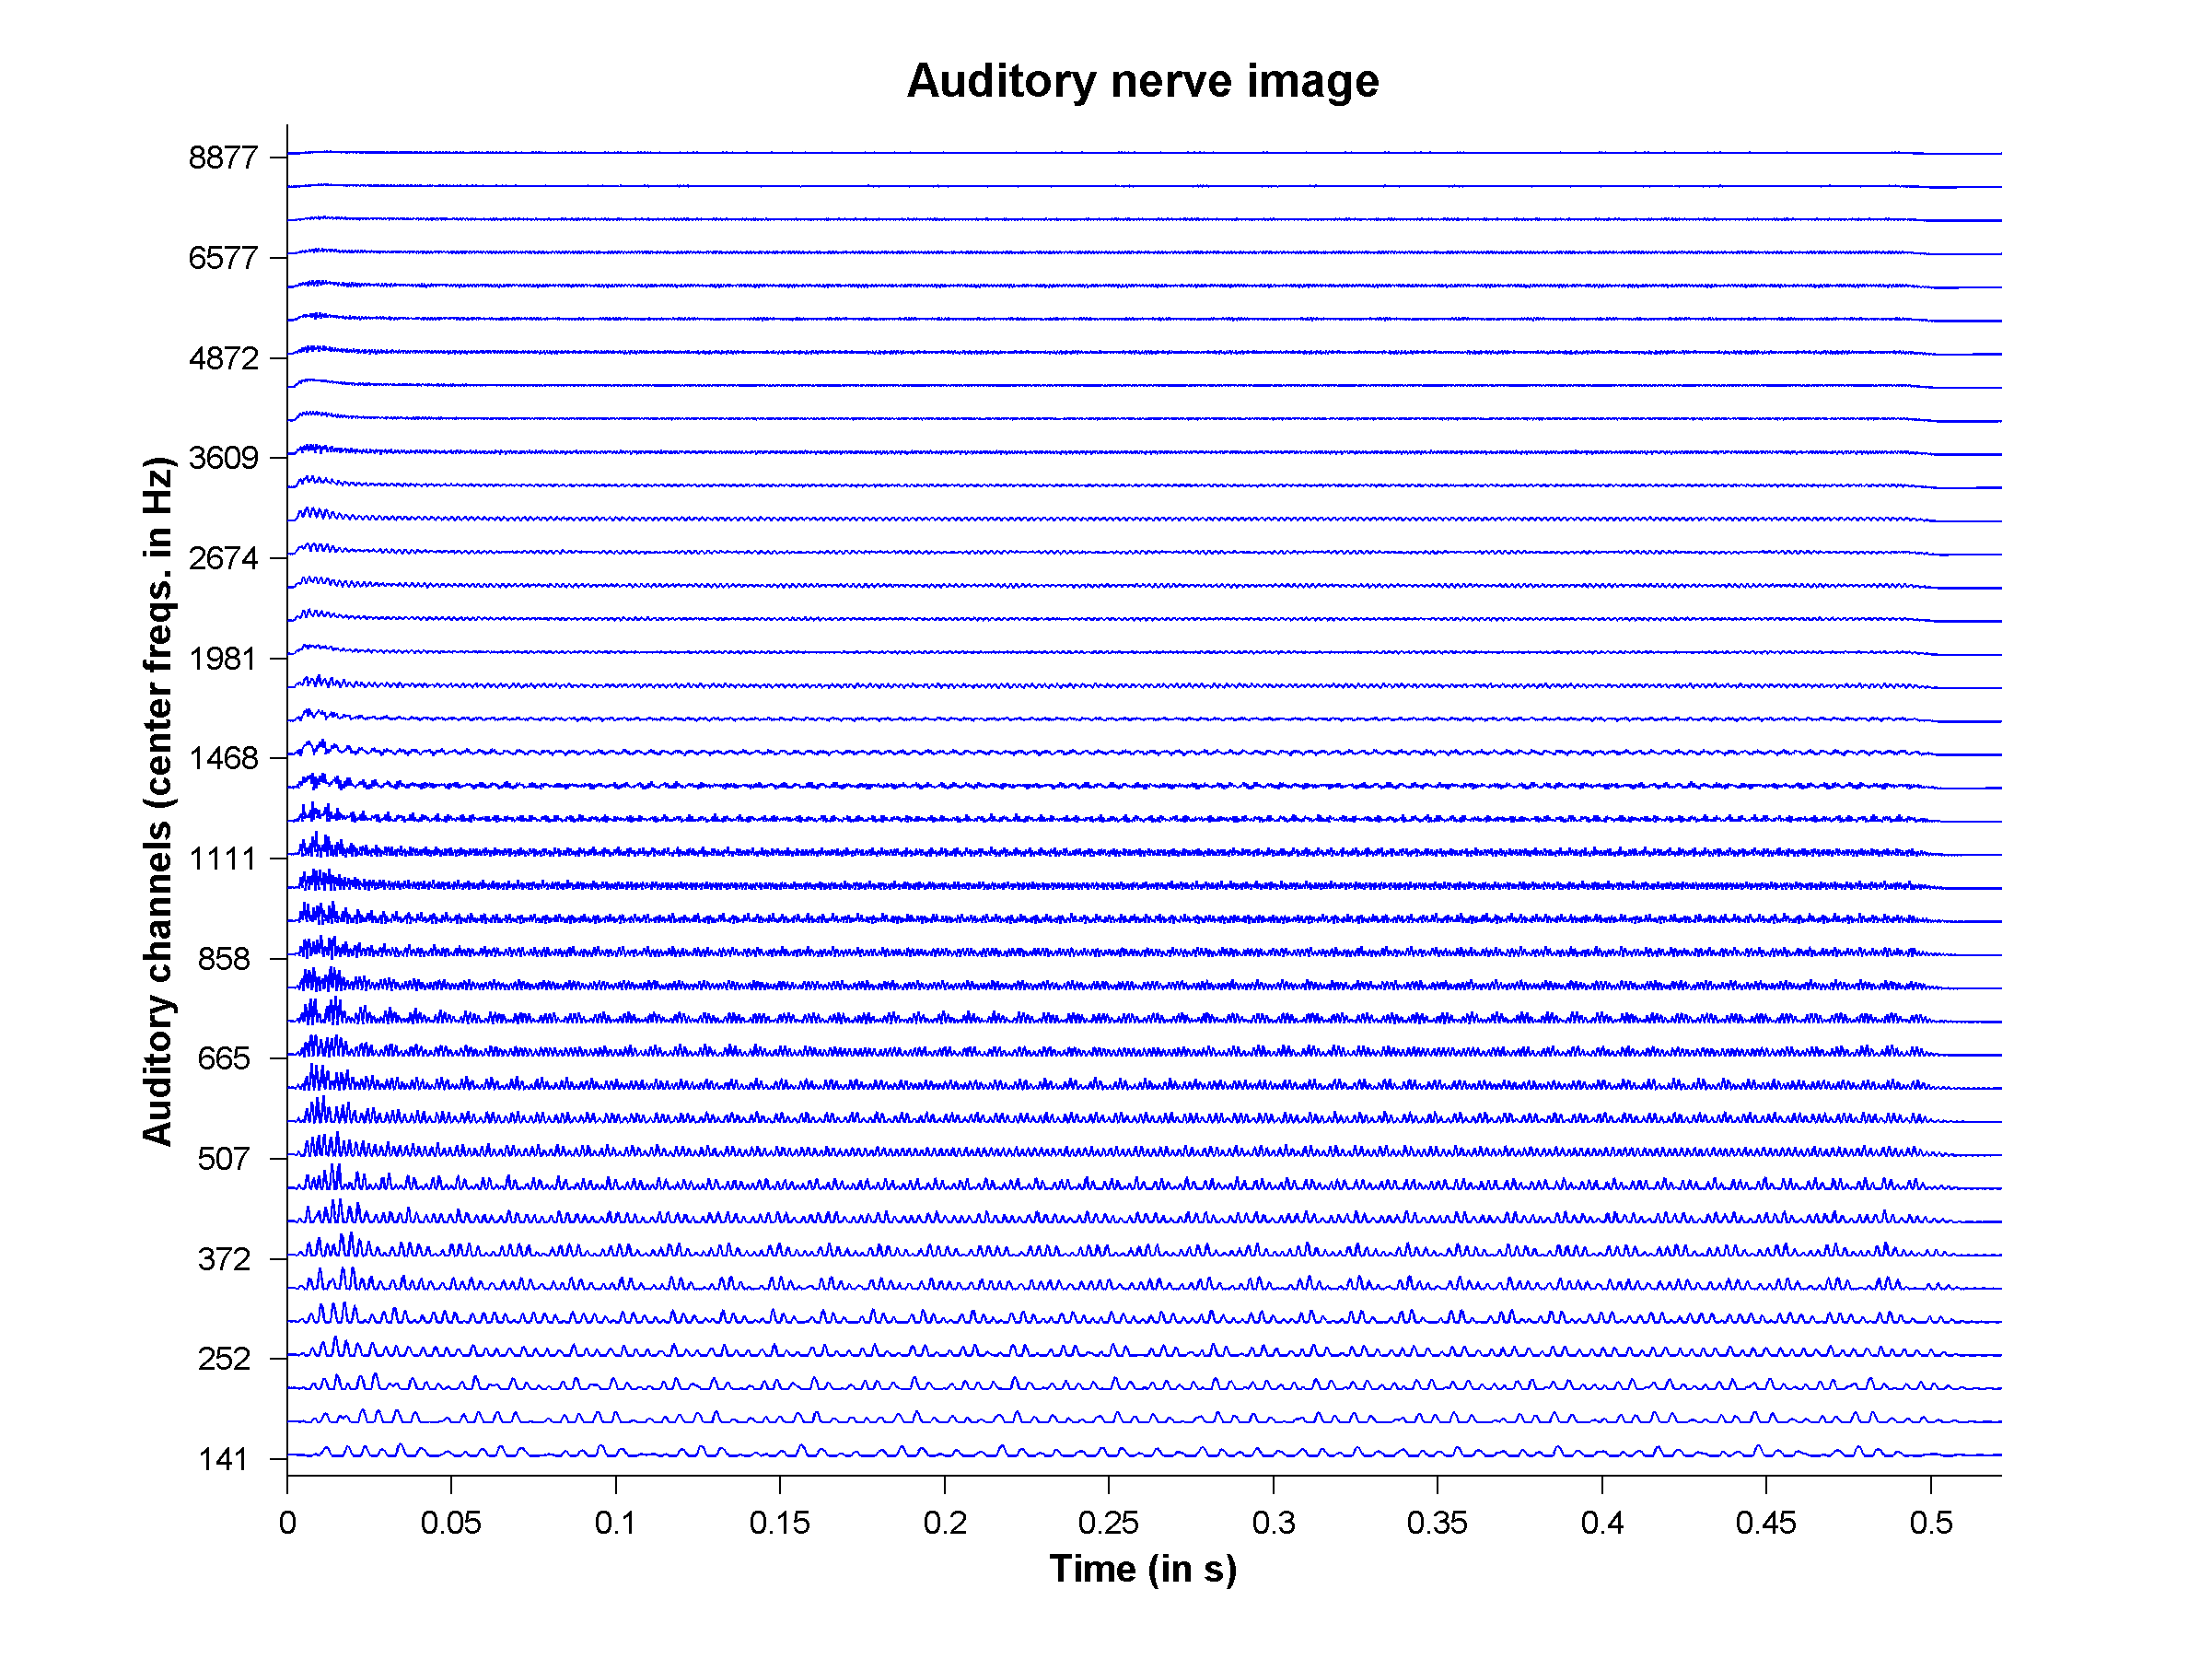
\includegraphics[width=\IPEMDefaultFigureWidth]{Graphics/ShepardCChordANI}
    \caption{Top: waveform of a C major chord using Shepard tones. Bottom: primary image}
    \label{Fig:ShepardCChordANIandAudioSignal}
\end{figure}

% --------------------------------------------------------------------------------

% --------------------------------------------------------------------------------
% --------------------------------------------------------------------------------
\newpage
\section{Roughness Module}
% --------------------------------------------------------------------------------

% Make general target
\hypertarget{Concepts:RoughnessModule}{}

% Make target for following functions:
\hypertarget{Concepts:IPEMRoughnessFFT}{}

\subsection{Introductory description}
% --------------------------------------------------------------------------------

The Roughness Module (RM) calculates the roughness (or
equivalently: the sensory dissonance) of a sound. Roughness is
considered to be a sensory process highly related to texture
perception. Hence, in our global chart of image transformation
modules it is localized in the top left (texture and sensory
based) section of figure \ref{Fig:ModulesRM}.
\begin{figure}[h]
    \centering
    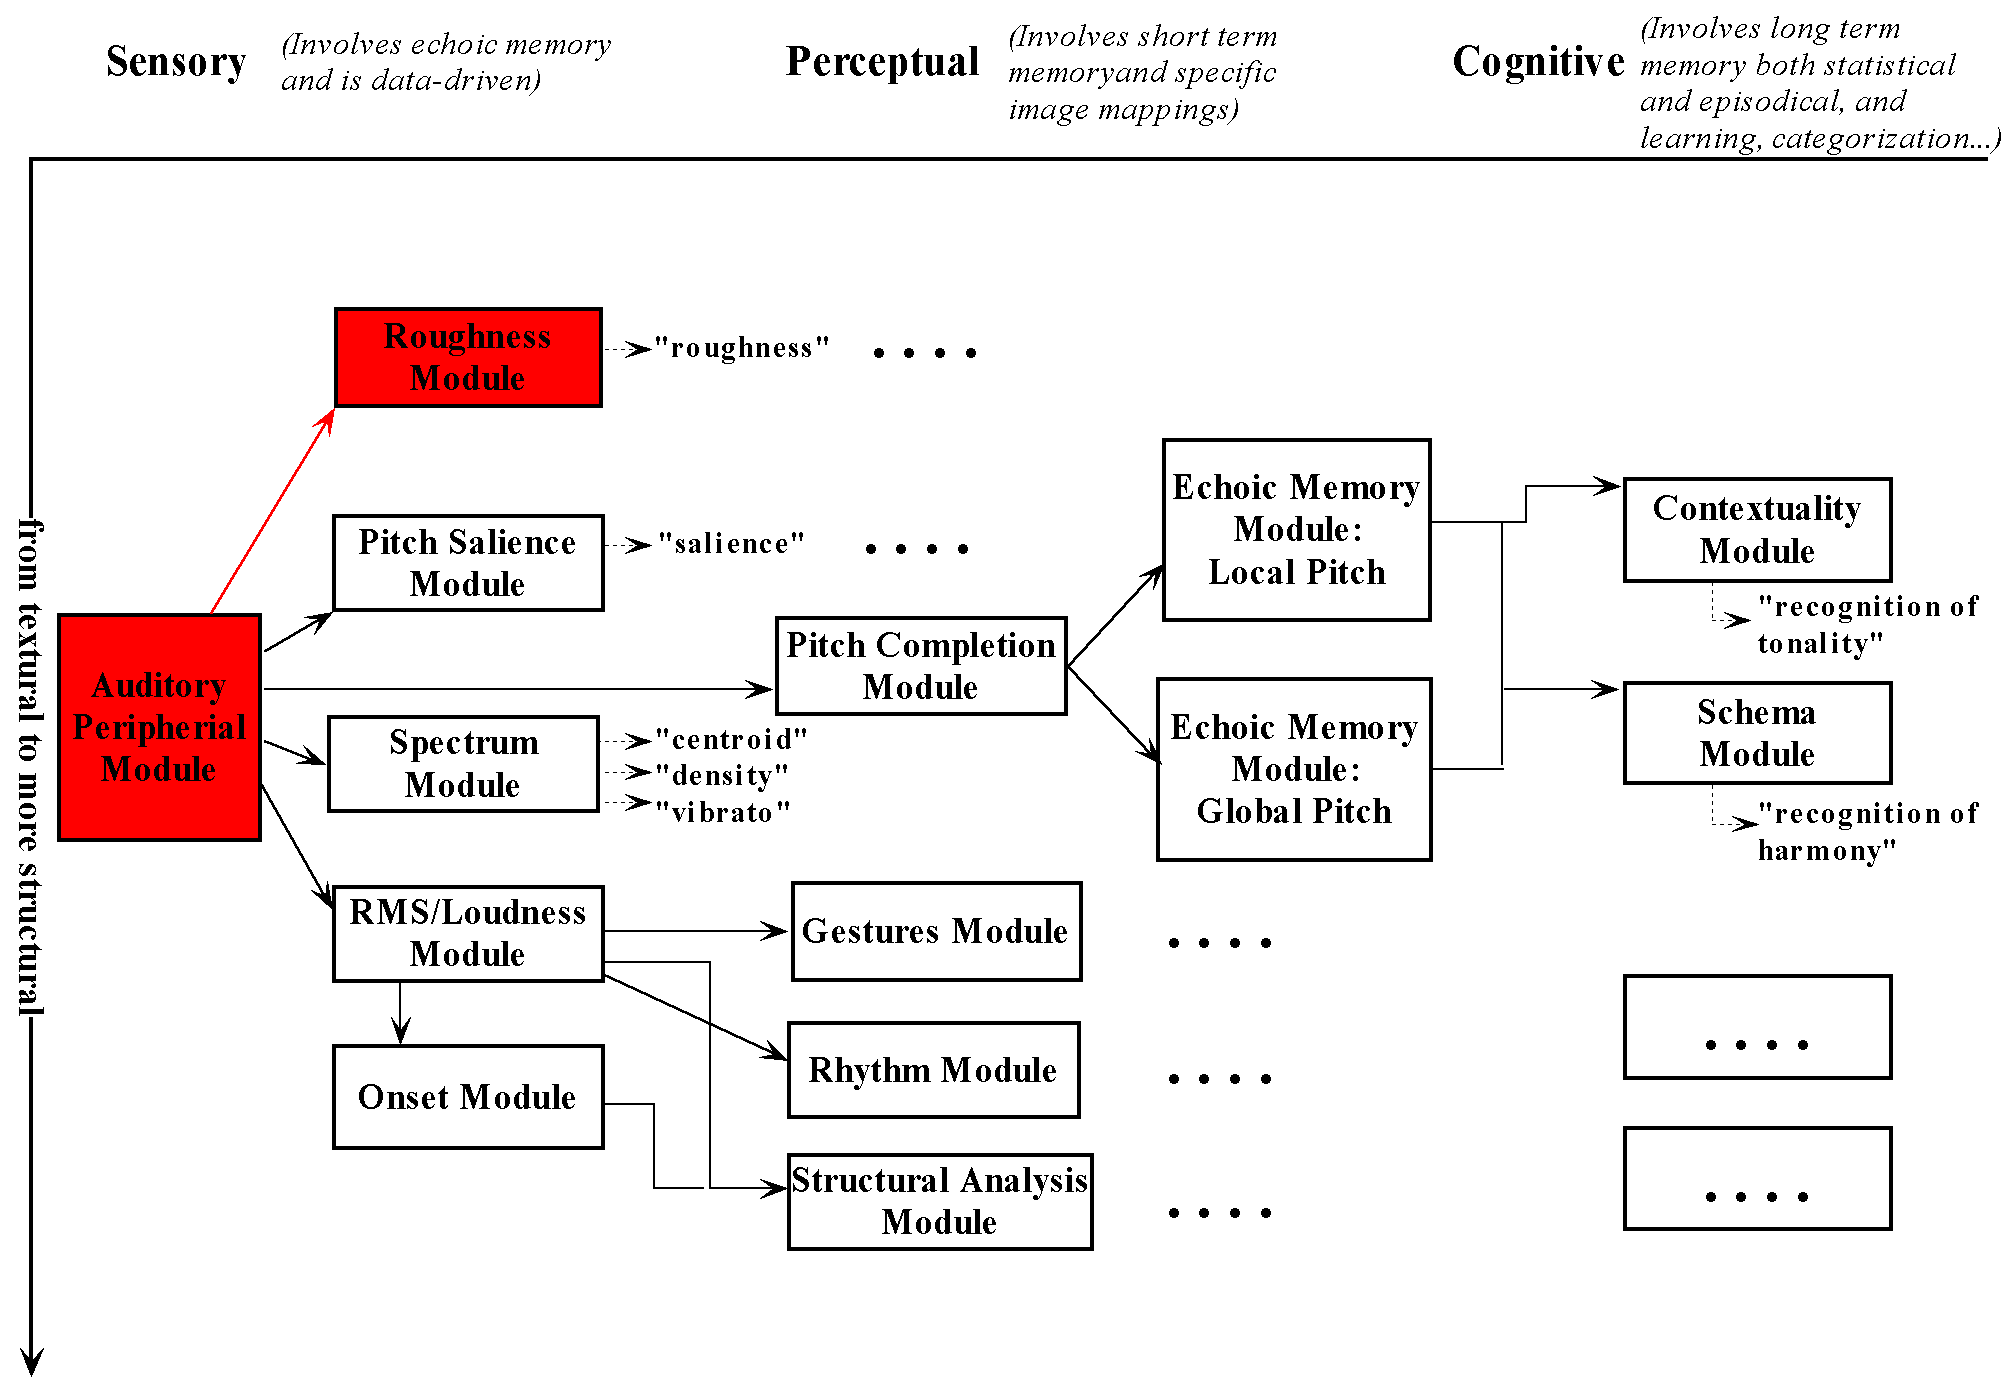
\includegraphics[width=\textwidth]{Graphics/ModulesRM}
    \caption{Chart of image transformation modules, with RM highlighted}
    \label{Fig:ModulesRM}
\end{figure}

The module takes sound as input (fig. \ref{Fig:RMModule}) and
produces a roughness estimation. The estimation should be
considered an inference.
\begin{figure}[h]
    \centering
    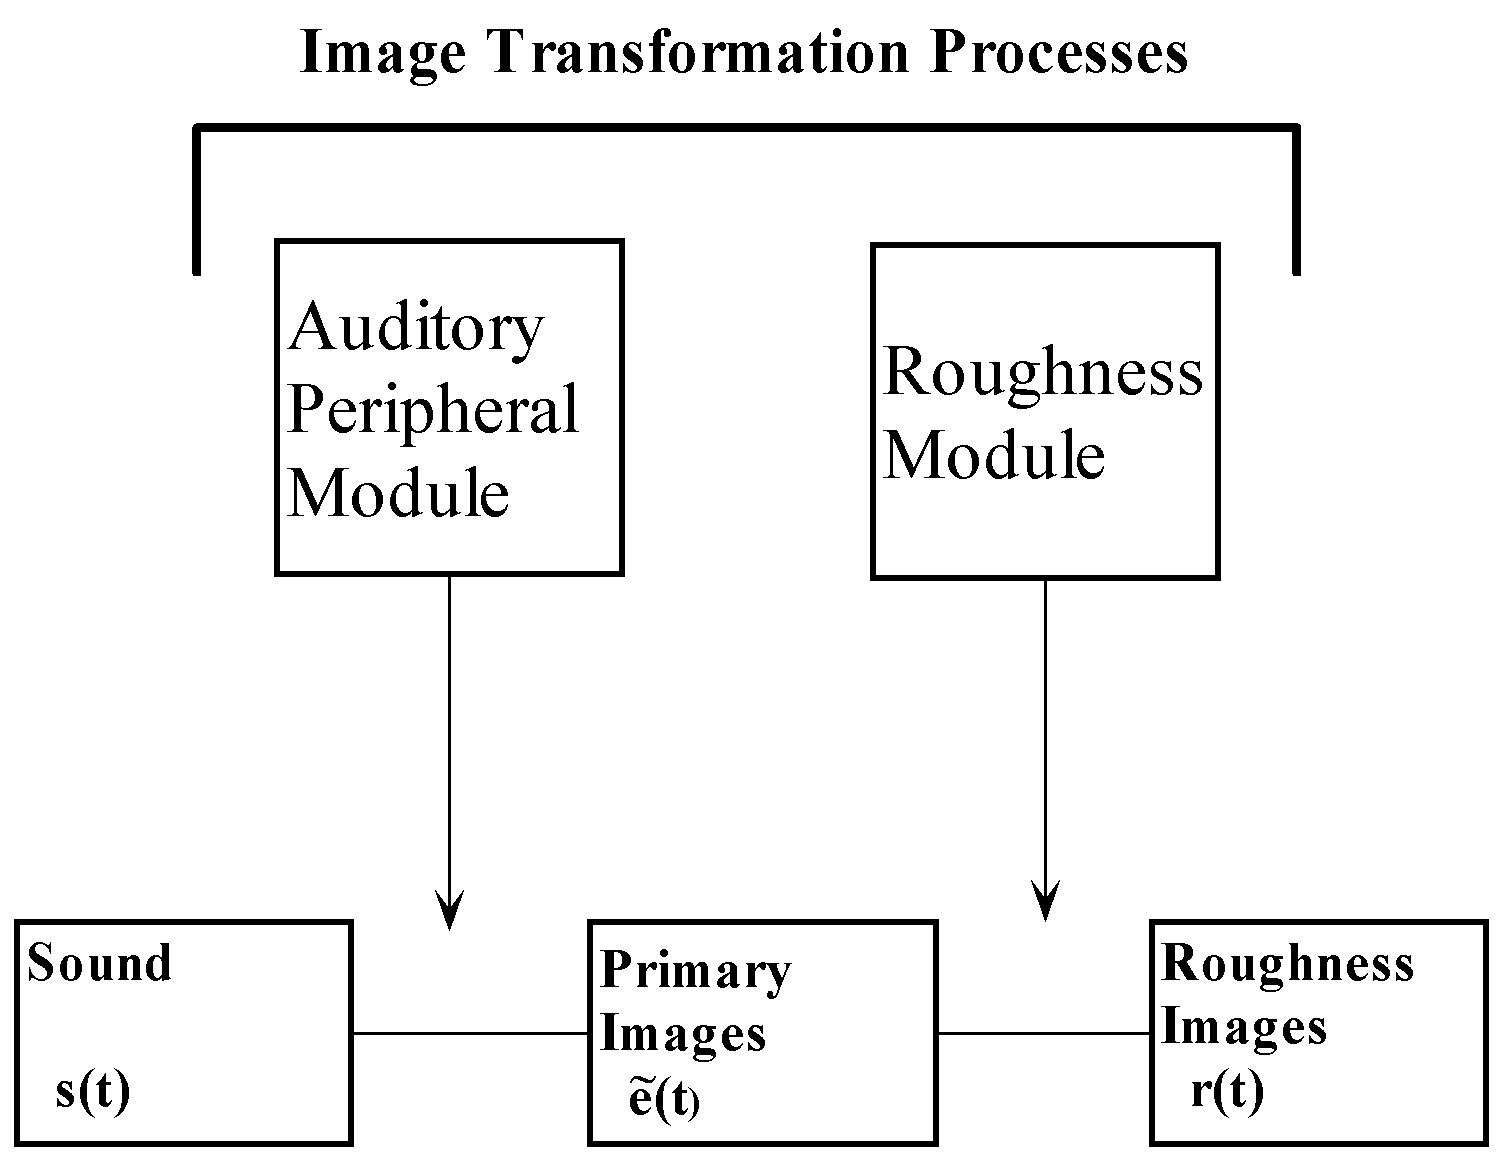
\includegraphics[width=\IPEMDefaultFigureWidth]{Graphics/RMModule}
    \caption{Image Transformation Process: Roughness Module}
    \label{Fig:RMModule}
\end{figure}
However, the module offers more than just an inference. The
visualization and calculation method of this module is based on
\citeA{inproceedings:Leman:DAFx:2000} where roughness is
defined as the energy of the relevant beating frequencies in the
auditory channels. The model is called the synchronization index
model of roughness and it is based on phase-locking to frequencies
that are present in the neural patterns. The synchronization index
model allows a straightforward visualization of the energy
components underlying roughness, in particular (i) with respect to
auditory channels, and (ii) with respect to phase-locking
synchronization (= the synchronization index for the relevant
beating frequencies on a frequency scale). That's why it is more
than just an inference. It assumes that neurons somehow extract
the energy of the beating frequencies and form internal images on
which the inference is based.

But what are beating frequencies? Take an amplitude modulated sine
wave with carrier frequency $f_c$ and modulation frequency $f_m$.
Such a signal has only three frequencies in the spectrum, in
particular $f_c$, $f_c-f_m$, and $f_c+f_m$. The beating frequency
is $f_m$. Now, in the auditory system, these frequencies are
introduced as effective beating frequencies into the spectrum of
the neural rate-code patterns. This is due to wave rectification
in the cochlea where the lower part of the modulated signal is cut
off, and as a result new frequencies are introduced of which the
most important ones correspond with the beating frequency $f_m$
and its multiples. As a matter of fact, neurons may synchronize
with these frequencies provided that they fall in the frequency
range where synchronization is physiologically possible. This
mechanism forms a physiological basis for the detection of beats
and hence, the sensation of roughness.

According to \citeA[p.~520-521]{Javel:88}, the synchronization
index represents the degree of phase-locking to a particular
frequency that is present in the neural pattern. The index can be
mathematically expressed as the (normalized) Fourier Series
coefficient at the frequency of interest. Using this concept, the
degree of roughness can be defined as the sum of the normalized
magnitudes or 'energies' of the relevant beating frequencies in
the Fourier spectrum.


\subsection{Functional-logical description}
% --------------------------------------------------------------------------------

Strictly speaking the roughness module realizes a transformation
from auditory nerve images onto roughness values. In a broad sense
the module starts from sound involving:
\begin{eqnarray}
    APM: s(t) \rightarrow \tilde{e}(t)\\
    RM: \tilde{e}(t) \rightarrow r(t)
\end{eqnarray}
where APM is the Auditory Peripheral Module which is used as the
first step, and RM is the transformation from the primary images
$\tilde{e}(t)$ to the roughness values $r(t)$ (our Roughness
Module in the strict sense). The latter are scalar values which we
can compare with human behavioral outputs.

\subsection{Signal processing description}
% --------------------------------------------------------------------------------

The synchronization index model calculates roughness in terms of
the 'energy' of neural synchronization to the beating
frequencies. The 'energy' refers to a quantity which we derive
from the magnitude spectrum.

Since the beating frequencies are contained in the lower
spectral area of the neuronal pattern $e(t,c)$, the spectral
part we are interested in is defined as:
\begin{equation}
  B(t,f,c) ~=~ F(f,c)D(t,f,c)
\end{equation}
where $F(f,c)$ is a filter whose spectrum is depending on the
channel $c$, and $D(t,f,c)$ is the short-term spectrum in
channel $c$ which we define as:
\begin{equation}\label{E1}
  D(t,f,c)~=~\int_{-\infty}^{+\infty} e(t,c)w(t'-t)e^{-j2\pi
  ft'}~dt'
\end{equation}
where $e(t,c)$ is the neural pattern in channel $c$, and
$w(t'-t)$ is a (hamming) window. The \emph{magnitude} spectrum
is then defined as $\left|~D(t,f,c)~\right|$, and the
\emph{phase} spectrum as $\angle D(t,f,c)$.

In order to be able to reproduce the psychoacoustical data on
roughness, the filters $F(f,c)$ should be more narrow at auditory
channels where the center frequency is below 800 Hz, and the
filters should be attenuated for high center frequencies as
well. The proposed set of filters $F(f,c)$ are shown in figure
\ref{Fig:Filters}. Small changes in parameters do not have a
dramatic effect on the performance of the model.

\begin{figure}[ht]
    \centering
    \includegraphics[width=\IPEMDefaultFigureWidth]{Graphics/Filters}
    \caption{Filters become more narrow in the lower auditory channels.}
    \label{Fig:Filters}
\end{figure}



$B(t,f,c)$ represents the \emph{spectrum} of the neural
synchronization to the beating frequencies in channel $c$. The
\emph{synchronization index} of the beating frequencies is then
defined as the normalized magnitude:
\begin{equation}
  I(t,f,c) ~=~ \left |~ \frac{B(t,f,c)}{D(t,0,c)}~\right |
\end{equation}
where $I(t,f,c)$ is the normalized magnitude in channel $c$.
$D(t,0,c)$ is the DC-component of the whole signal in channel
$c$.

The short-term \emph{'energy'} spectrum of the neural
synchronization to beating frequencies in a particular auditory
channel $c$ is defined as:
\begin{equation}\label{Rspectrum}
\textbf{B}(t,f,c) ~=~ I(t,f,c) ~^{1.6}~=~ {\left |~
\frac{B(t,f,c)}{D(t,0,c)}~\right |~}^{1.6}
\end{equation}

%\item
% the energy spectrum of the neural synchronization to
% beating frequencies over all auditory
% channels is:
%\begin{equation}\label{R2}
%\textbf{B}(t,f) ~=~ \sum_{c=1}^{C} \textbf{B}(t,f,c)~ w_c
%\end{equation}
%where $w_c$ is the weighting factor defined for each channel.
%\item
% the overall energy of the neural synchronization to beating frequencies in one channel is:
% \begin{equation}\label{R3}
%E_\textbf{B}(t,c) ~=~ \int_{f=-\infty}^{+\infty}
%\textbf{B}(t,f,c)~df
%\end{equation}
%\end{itemize}



We then define the following relationships for the calculation of
roughness:
\begin{equation}\label{R5}
\begin{array}{lll}
  R_\textbf{B}(t)&~=~\int \textbf{B}(t,f)~df
                 &~=~\int \sum_{c=1}^{C}
                 \textbf{B}(t,f,c)~df\\\\
                 &~=~\sum_{c=1}^{C} \textbf{B}(t,c)
                 &~=~\sum_{c=1}^{C} \int  \textbf{B}(t,f,c)~df\\
\end{array}
\end{equation}
where $R_\textbf{B}(t)$ is the roughness at time $t$. The
roughness is obtained by an integration of the 'energy' over all
frequencies, as well as over all channels. This definition
implies a proper visualization, one along the axis of auditory
channels and one along the axis of the (beating) frequencies.

%We now assume that roughness is related to the 'energy' of this
%normalized Fourier transform.
%
%In particular, roughness is calculated in the individual channels
%and the total roughness is the sum of the channel roughnesses.
%Given the above discussion, it will be possible to visualize the
%contribution of the synchronization energy along the axis of the
%auditory channels, as well as along the axis of the beating
%frequencies.






%Given the general concept as described above, the implementation
%requires a specification of the filters $F(f,c)$. In the present
%modeling, we choose elegance as an important criterium to
%describe the filters mathematically.
%The form of the filter
%$F'(f,c)$ has first been defined according to the following
%formula's:
%\begin{equation}
%F'(f,c)~=~e^{-8 \frac{f}{f_B}} \left [~1 - cos(2 \pi
%\frac{f}{10f_B}) ~\right ] w(c)
%\end{equation}
%where $f_B$ is the frequency range of the filter and $f$ is
%running from 1 to $f_B$, $w(c)$ is a weight depending on the
%channel $c$. The weight takes into account a linear decrease of
%the impact of the filter depending on the auditory channel number:
%\begin{equation}
%w(c)~=~1-\frac{0.55c}{C})
%\end{equation}
%with c running from 1 to C (=40). The frequency range $f_B$ is
%defined such that it is narrow for the lower auditory channels
%below 800 Hz, broad at about 1000 Hz and again slightly more
%narrow at frequencies higher than 1500 Hz.
%
%A sigmoid function has been defined according to
%%(fig.~\ref{Sigmoid}):
%\begin{equation}\label{Sigmoid}
%S~=~ \frac{(\frac{c}{C})^{.2}} {0.04 + (\frac{c}{C})^{2.45} -
%0.007c}
%\end{equation}
%The sigmoid function is used to define the frequency range as:
%\begin{equation}
%f_B(c) = 10 + (300 * \frac{S}{S_{max}} );
%\end{equation}
%It means that the frequency range of the filter in the lowest
%auditory channel is 10 Hz, and that this range is at most 310 Hz
%(around 1000 Hz). The values of S are normalized so that the
%maximum value of $\frac{S}{S_{max}}$ is equal to one.
%
%%\begin{figure}
%%  \centering
%%  \includegraphics{figures/Sigmoid}
%%  \caption{Sigmoid function}\label{Sigmoid}
%%\end{figure}
%Given the set of filters $F(f,c)$, the sigmoid function
%(\ref{Sigmoid}) has also been used to define where the maximum of
%the filter should be located. Data indicate that the maximum
%around 1000 Hz is at about 70 Hz. It is lower for low auditory
%channels.
%\begin{equation}
%f_M(c) = 20 + (52 * \frac{S}{S_{max}} );
%\end{equation}
%This function starts at 20 Hz and the maximum is obtained at 72
%Hz.
%
%The precise location of the filter shape $F'(f,c)$ on the
%frequency axis is then determined by placing its maximum at
%$f_M(c)$.



%Figure \ref{Filters} shows an array of such filters.
%\begin{figure}
%  \centering
%  \includegraphics{figures/Filters}
%  \caption{Filters become more narrow in the lower auditory channels}\label{Filters}
%\end{figure}


\subsection{Implementation}
% --------------------------------------------------------------------------------

\begin{tabularx}{\linewidth}{llX}
\hyperlink{FuncRef:IPEMRoughnessFFT}{IPEMRoughnessFFT} & - & Calculates roughness using synchronization index model\\
\end{tabularx}


\subsection{Examples}
% --------------------------------------------------------------------------------

The function
\hyperlink{FuncRef:IPEMRoughnessFFT}{IPEMRoughnessFFT}
has a number of input parameters. To calculate the roughness of
the wav-file \emph{SchumannKurioseGeschichte.wav} do:\\

\IPEMCodeExtract{[ANI,ANIFreq,ANIFilterFreqs] = ...\\IPEMCalcANIFromFile('SchumannKurioseGeschichte.wav');}\\

\IPEMCodeExtract{IPEMRoughnessFFT(ANI,ANIFreq,ANIFilterFreqs,5,300,0.200,0.020,1);}\\

Notice that the toolbox functions are linked through the variables
\IPEMCodeExtract{ANI,ANIFreq,ANIFilterFreqs}. These variables are
the output of the Auditory Peripheral Module, and (part of) the
input to the Roughness Module. The resulting figure should be
similar to the one shown in figure \ref{Fig:RMRoughness}.\\

\begin{figure}[h]
    \centering
    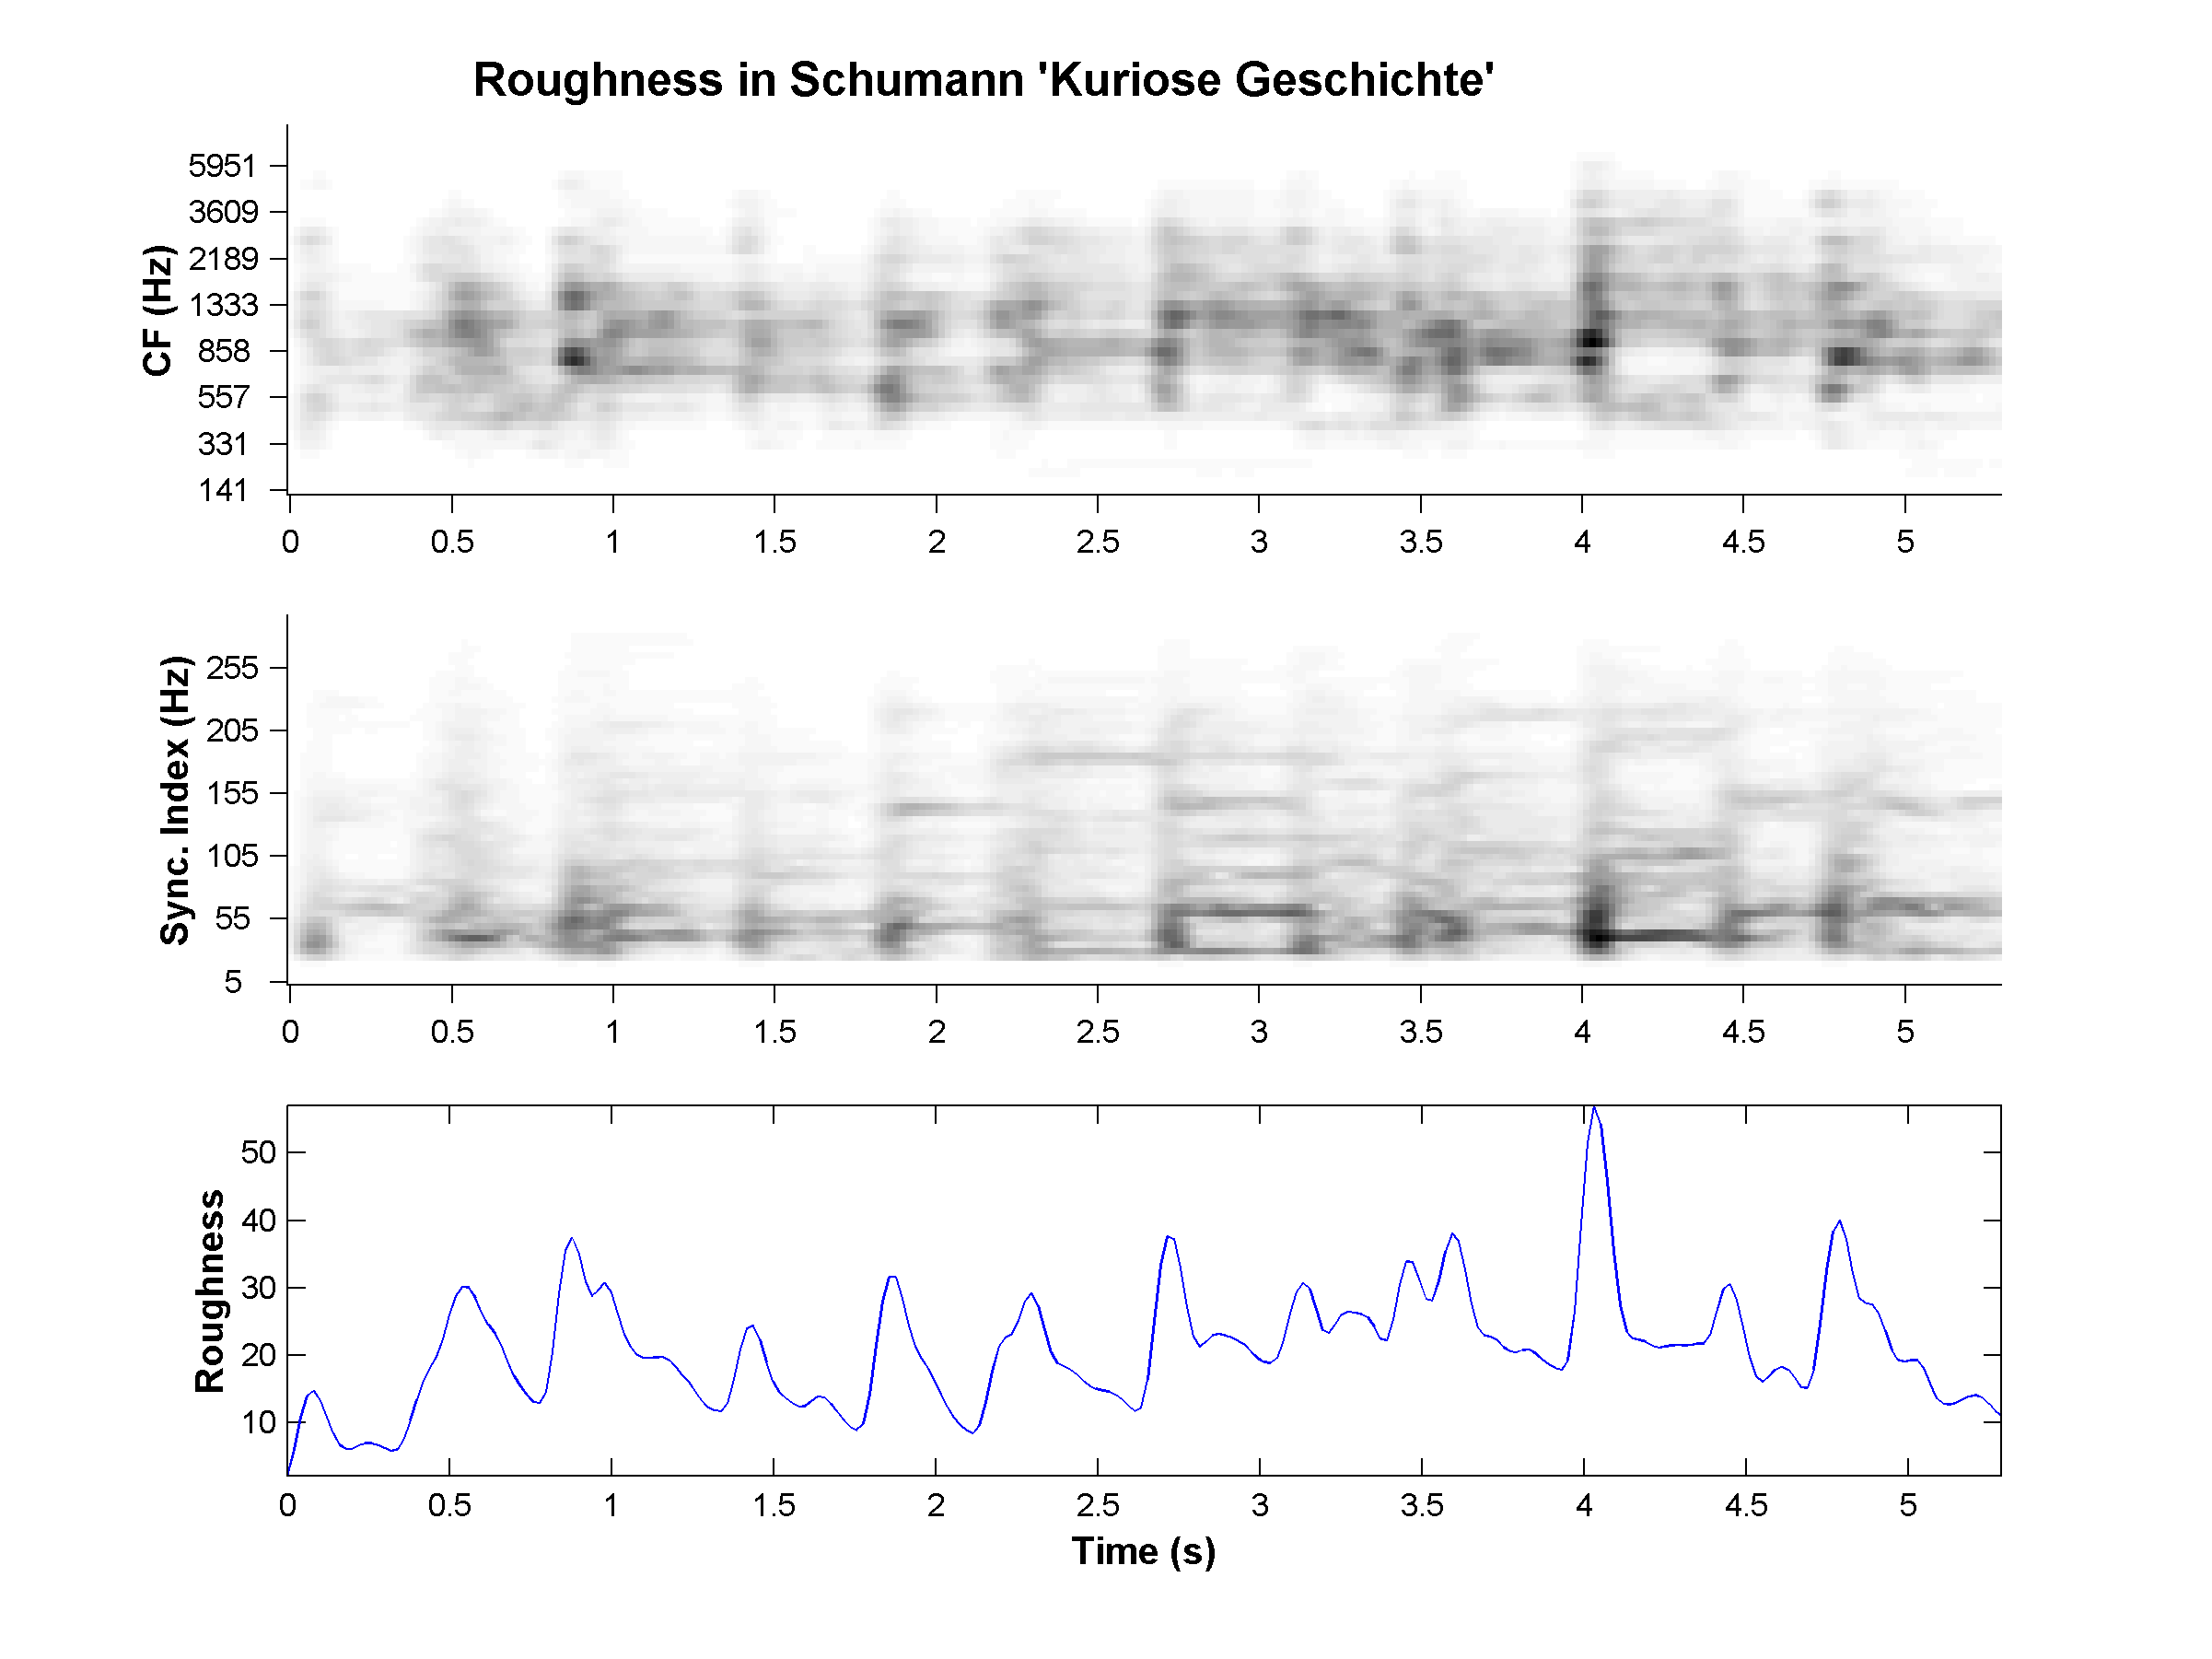
\includegraphics[width=\IPEMDefaultFigureWidth]{Graphics/RMRoughness}
    \caption{The upper panel shows the energy as distributed over the
    auditory channels, the middle panel shows the energy as
    distributed over the beating frequencies, the lower panel
    shows the roughness (which is the sum of either the upper or
    middle panel)}
    \label{Fig:RMRoughness}
\end{figure}

%See also \hyperlink{Chapter:ConceptsApplications}{Applications}
%for more elaborate examples.\\

% --------------------------------------------------------------------------------

% --------------------------------------------------------------------------------
% --------------------------------------------------------------------------------
\newpage
\section{Onset Module}
% --------------------------------------------------------------------------------

% Make general target
\hypertarget{Concepts:OnsetModule}{}

% Make target for following functions:
\hypertarget{Concepts:IPEMCalcOnsets}{}
\hypertarget{Concepts:IPEMCalcOnsetsFromANI}{}
\hypertarget{Concepts:IPEMDoOnsets}{}
\hypertarget{Concepts:IPEMOnsetPattern}{}
\hypertarget{Concepts:IPEMOnsetPatternFilter}{}
\hypertarget{Concepts:IPEMOnsetPeakDetection}{}
\hypertarget{Concepts:IPEMOnsetPeakDetection1Channel}{}
\hypertarget{Concepts:IPEMSnipSoundFileAtOnsets}{}

\subsection{Introductory description}
% --------------------------------------------------------------------------------
The onset module (OM) finds the onsets of sound events. The module
takes sound as input and produces the moments where a new note,
chord or sound event is triggered in the musical signal. Its place
in the image transformation chart is shown in figure
\ref{Fig:ModulesOM}.
\begin{figure}[h]
    \centering
    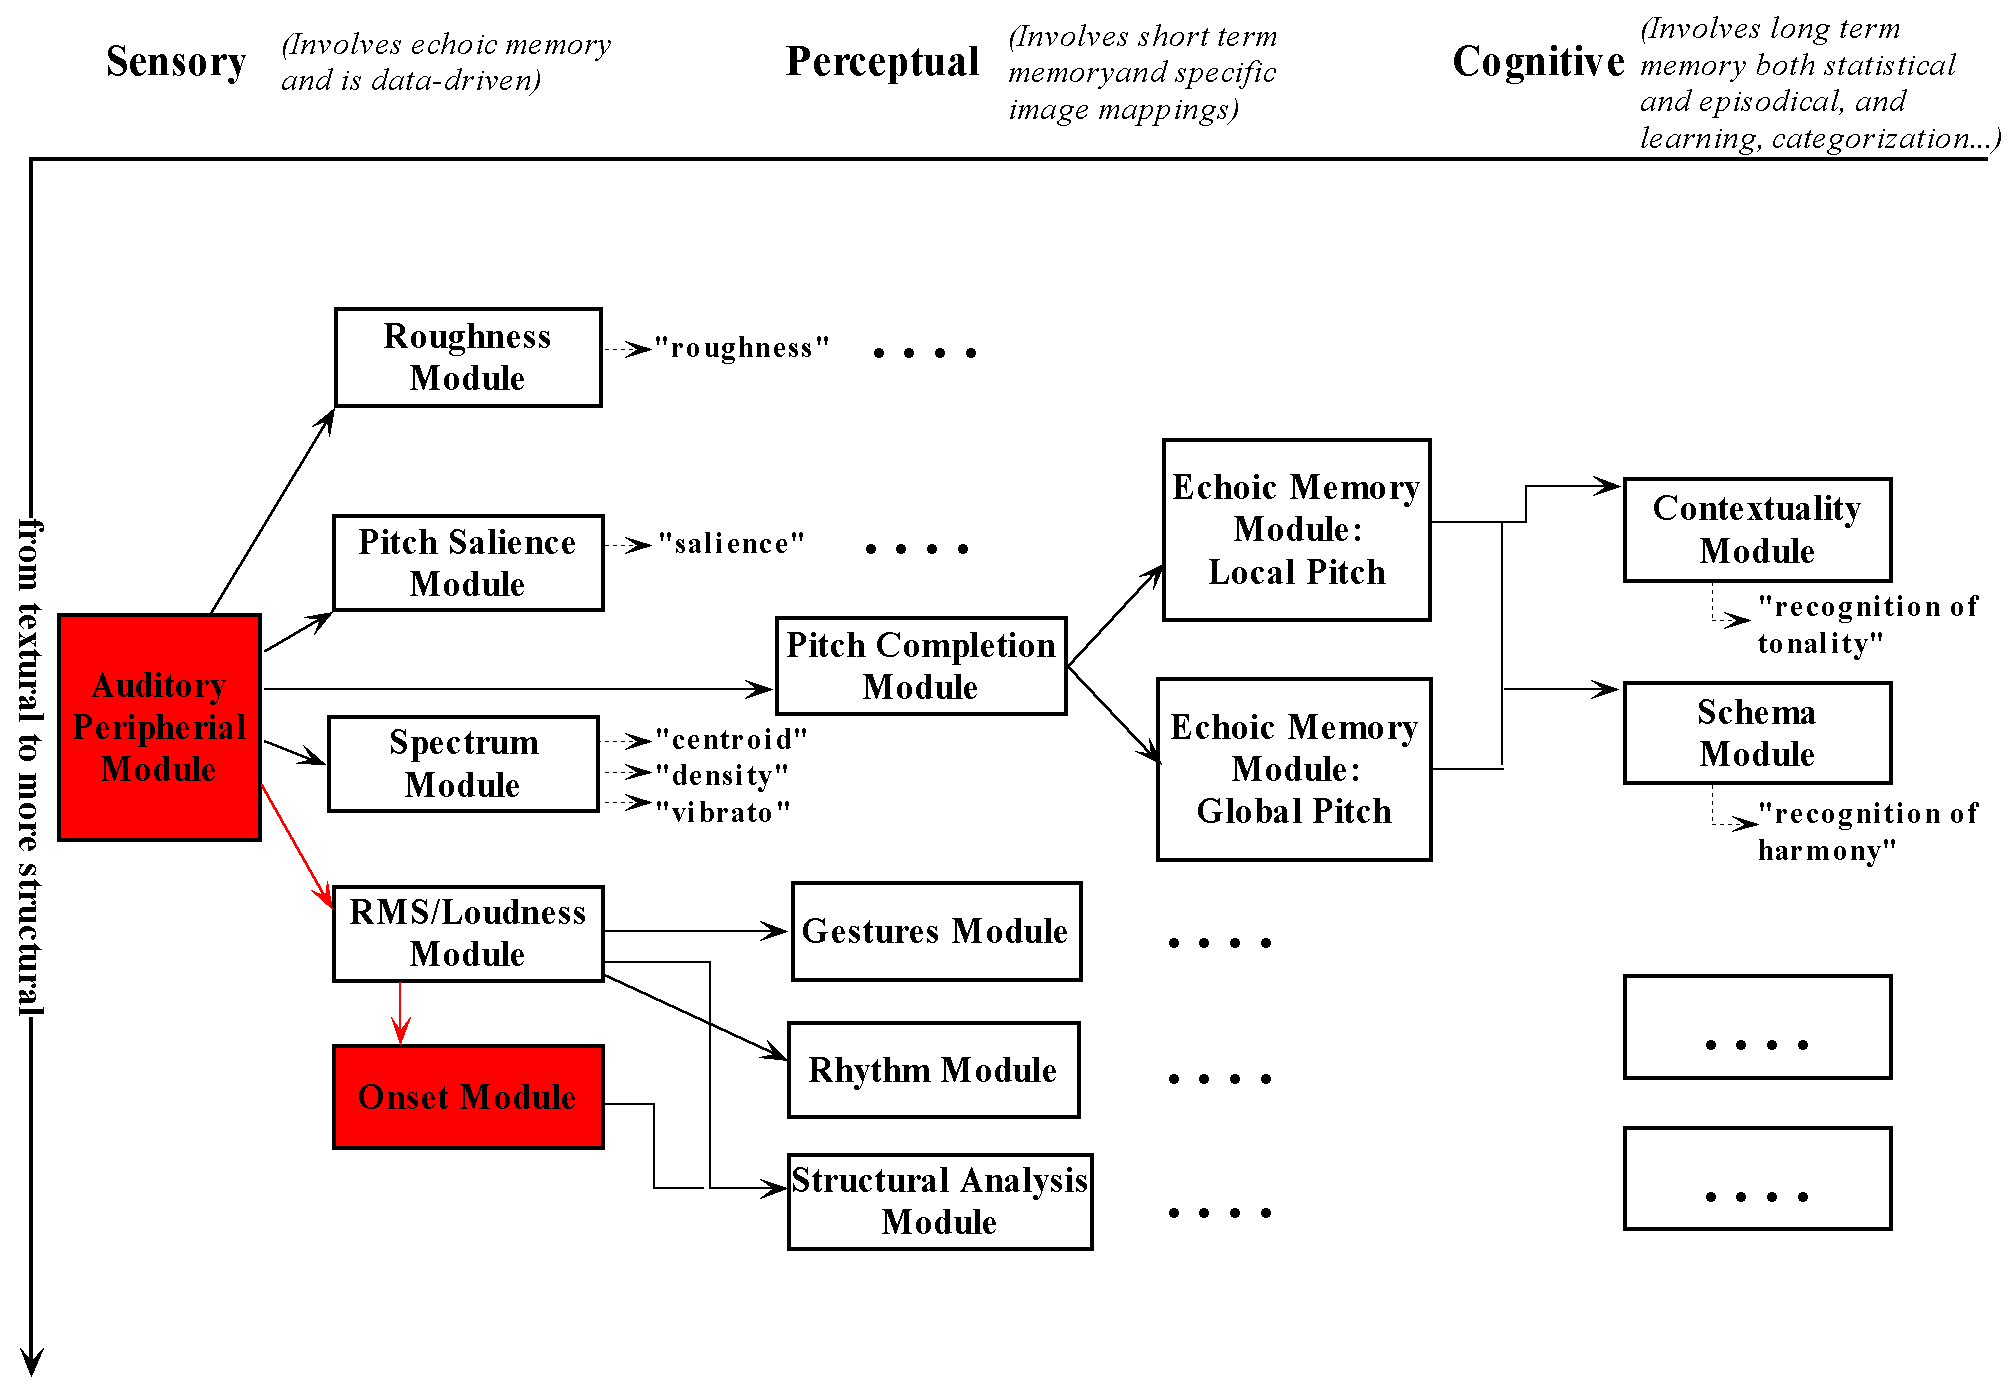
\includegraphics[width=\textwidth]{Graphics/ModulesOM}
    \caption{Chart of image transformation modules, with OM highlighted}
    \label{Fig:ModulesOM}
\end{figure}

The onset module analyzes the energy in the different auditory
channels. It extracts the relevant peaks and combines the results
for each channel to an overall onset estimation. Keep in mind that
onset detection is a rather difficult enterprise due to the fact
that some music instruments (violin, human voice, ...) have
gliding onsets which are hard to detect. Our onset module can be
used to chunk the frame-based representation into an event-based
representation. Figure \ref{Fig:OMModule} shows the modules
involved in the transformation process.
\begin{figure}[h]
    \centering
    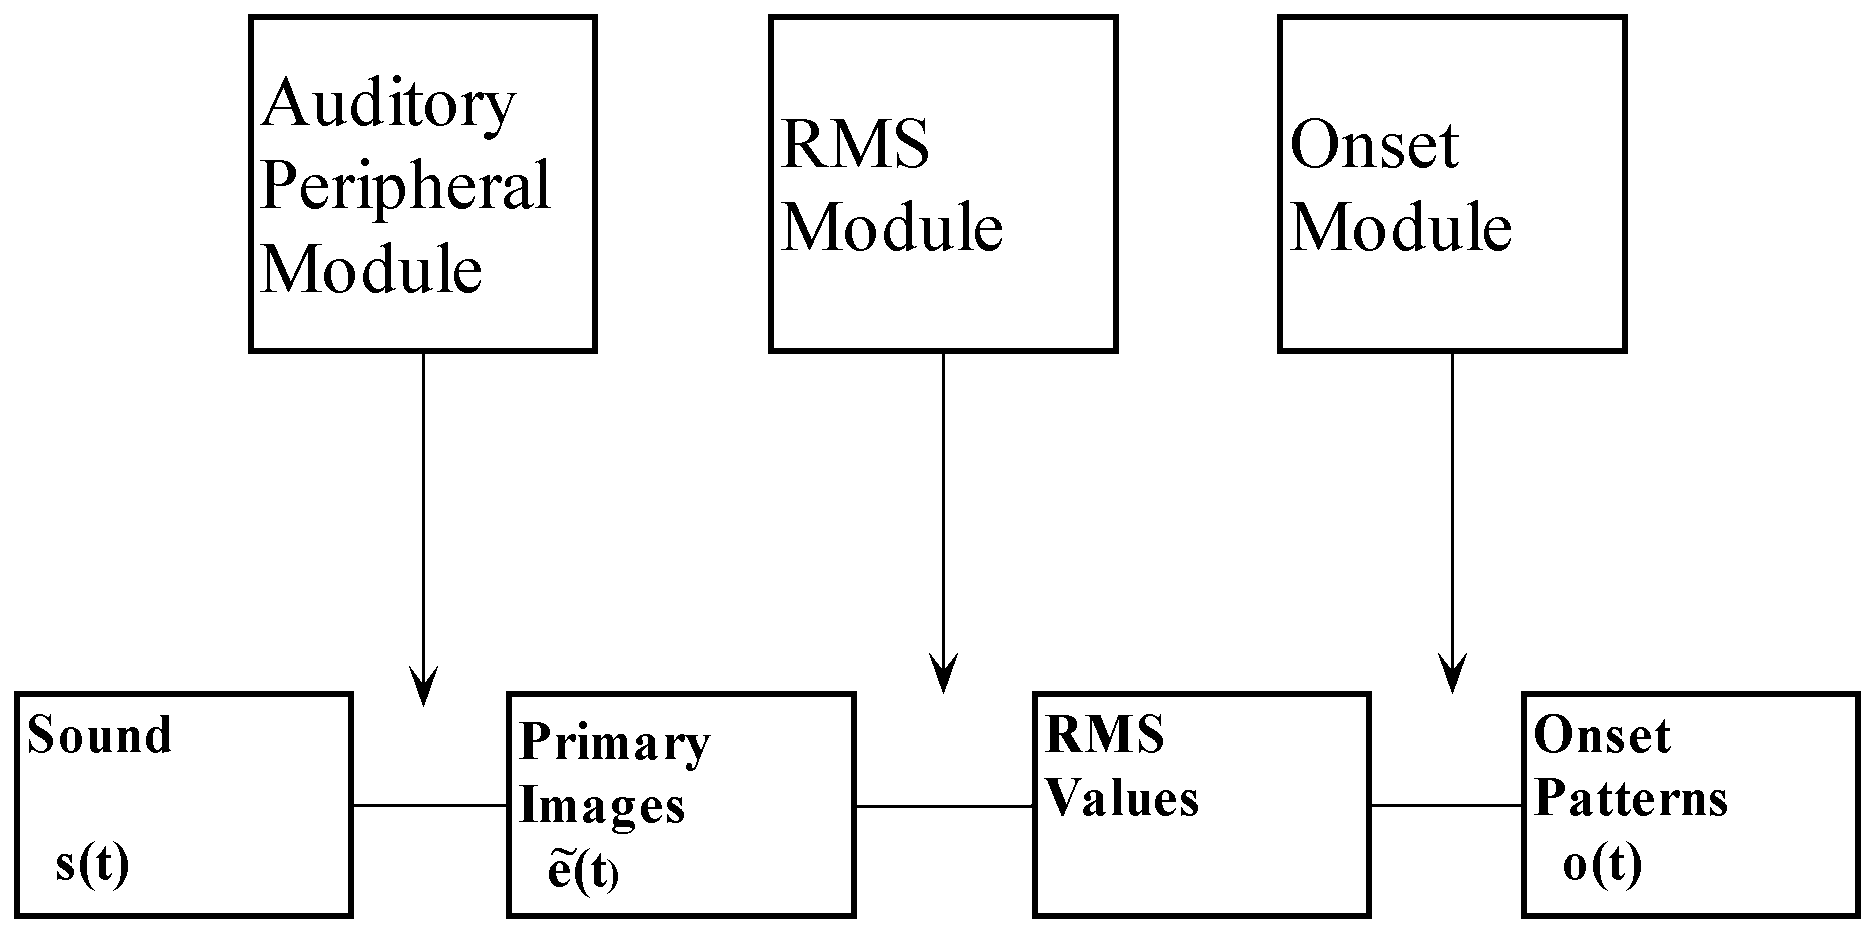
\includegraphics[width=\IPEMDefaultFigureWidth]{Graphics/OMModule}
    \caption{Modules involved for onset estimation.}
    \label{Fig:OMModule}
\end{figure}

\subsection{Functional-logical description}
% --------------------------------------------------------------------------------

The onset module involves:
\[APM: s(t) \rightarrow \tilde{e}(t)\]
\[RMS: \tilde{e}(t) \rightarrow \widetilde{rms}(t)\]
\[OM: \widetilde{rms}(t) \rightarrow o(t)\]
where APM provides the auditory nerve images and OM transforms
these images into the signal $o(t)$. A non-zero value in $o(t)$
corresponds to an onset at that moment, the value itself being
proportional to the estimated relevance of the onset.

\subsection{Signal processing description}
% --------------------------------------------------------------------------------

The algorithm used for detection of onsets consists of the
following steps:
\begin{enumerate}
\item Calculation of auditory nerve image.\\
    The auditory nerve image is calculated
    using the \hyperlink{Concepts:AuditoryPeripheralModule}{Auditory Peripheral Module}.
\item Calculation of RMS.\\
    For each of the channels in the ANI, the root mean square values are calculated using
    a frame size of 0.029 s and a frame step of 0.0058 s.
    For each frame $F$ in each channel, an RMS value is calculated according to:
    \begin{displaymath}
    RMS = \sqrt{\frac{\displaystyle \sum_{i=1}^{N}{F_{i}^2}}{N}}
    \end{displaymath}
    where $N$ = frame width in samples, and $F_{i}$ is the i-th sample of frame
    $F$.
    There is a toolbox function for the calculation of RMS values,
    see \hyperlink{FuncRef:IPEMCalcRMS}{IPEMCalcRMS}.
\item Low pass filtering.\\
    Each of these RMS-averaged channels is filtered with a second-order low pass Butterworth filter
    with a cutoff frequency of 15 Hz. This is done to reduce small, irrelevant peaks in the RMS signal.
\item Peak detection.\\
    Detection of relevant peaks in each channel is the tricky
    part....
    We start with all true peaks: moments where the first derivative goes from positive to negative.
    Then, the following approach is used for deciding whether a peak in a channel should be kept as an
    onset candidate for that channel:
    \begin{itemize}
    \item ignore everything below a certain threshold
    \item only keep peaks that are significantly bigger than their neighbors
    \item apply a mask so that following peaks due to irrelevant vibrations are thrown out
    \item for all remaining peaks, keep the biggest ones within a certain neighborhood, but only
          if it's big enough compared to the median value at that point
    \end{itemize}
\item Application of integrate-and-fire neural network.\\
    The contribution of this part is to cluster the peaks detected in the previous step over
    all channels and over time.
    This algorithm is based on an article by \citeA{Smith:1996}.
    One integrate-and-fire neuron is used per channel.
    Each neuron receives input from a set of
    adjacent channels, accumulates its input over time
    and its output is fed back to a number
    of adjacent neurons.
    The neuron dynamics are given by:
    \begin{displaymath}
    \frac{dA}{dt} = I(t) - diss\times{A} \qquad \textrm{with:
        \begin{tabular}[t]{l}
            $A$ = neurons' accumulated value \\
            $I$ = input \\
            $diss$ = dissipation factor
        \end{tabular}
        }
    \end{displaymath}

    If a neurons' accumulated value exceeds a certain threshold, it fires and the accumulated value
    is reset to zero. After firing, the neuron becomes insensitive to input for some period,
    called the refractory period. This configuration produces a sharp bursts of spikes when a
    number of channels provide evidence for onsets.
\item Final filtering.\\
    The onset pattern is finally filtered using the following approach:
    an onset is detected at a certain moment\\
    \begin{tabular}[t]{l}
        - if a certain number of channels detected an onset within
        a specific period of time, and\\
        - if the moment falls at least a minimum period of time
        behind the last detected onset\\
    \end{tabular}
\end{enumerate}

The result of these steps is a signal where a non-zero value
indicates the presence of an onset. To get an indication for the
relevance of a specific onset, we have used the number of
channels that detected an onset divided by the total number of
channels.

\subsection{Implementation}
% --------------------------------------------------------------------------------

\begin{tabularx}{\linewidth}{llX}
\hyperlink{FuncRef:IPEMCalcOnsets}{IPEMCalcOnsets} & - & Calculates onsets of sound signal\\
\hyperlink{FuncRef:IPEMCalcOnsetsFromANI}{IPEMCalcOnsetsFromANI} & - & Calculates onsets starting from an ANI\\
\hyperlink{FuncRef:IPEMDoOnsets}{IPEMDoOnsets} & - & Calculates onsets of sound file\\
\hyperlink{FuncRef:IPEMOnsetPattern}{IPEMOnsetPattern} & - & Integrate-and-fire neural net for onset detection\\
\hyperlink{FuncRef:IPEMOnsetPatternFilter}{IPEMOnsetPatternFilter} & - & Filters onset detection peak pattern\\
\hyperlink{FuncRef:IPEMOnsetPeakDetection}{IPEMOnsetPeakDetection} & - & Detects possible onset peaks in multi-channel signal\\
\hyperlink{FuncRef:IPEMOnsetPeakDetection1Channel}{IPEMOnsetPeakDetection1Channel} & - & Detects possible onset peaks in single channel\\
\hyperlink{FuncRef:IPEMSnipSoundFileAtOnsets}{IPEMSnipSoundFileAtOnsets} & - & Cuts sound file in segments at onsets\\
\end{tabularx}


\subsection{Examples}
% --------------------------------------------------------------------------------

To extract the onsets from
\IPEMSound{Sounds/SchumannKurioseGeschichte.wav}{Schumann's
Kuriose Geschichte}, use the following expression:\\

\begin{IPEMCodeEnvironment}
[Ts,Tsmp] = IPEMDoOnsets('SchumannKurioseGeschichte.wav');
\end{IPEMCodeEnvironment}\\

You can of course split the module in the several subparts. For
example, if you first process the file with the Auditory
Peripheral Module, and then apply the onsets module, you could
use:\\

\begin{IPEMCodeEnvironment}
[ANI,ANIFreq,ANIFilterFreqs] = IPEMCalcANIFromFile('SchumannKurioseGeschichte.wav');
\newline [OnsetSignal,OnsetFreq] = IPEMCalcOnsetsFromANI(ANI,ANIFreq);
\end{IPEMCodeEnvironment}\\

Figures \ref{Fig:OnsetsANIAndRMS} to \ref{Fig:OnsetsSegmentation}
illustrate the different steps for this particular example.

\begin{figure}[h]
    \centering
    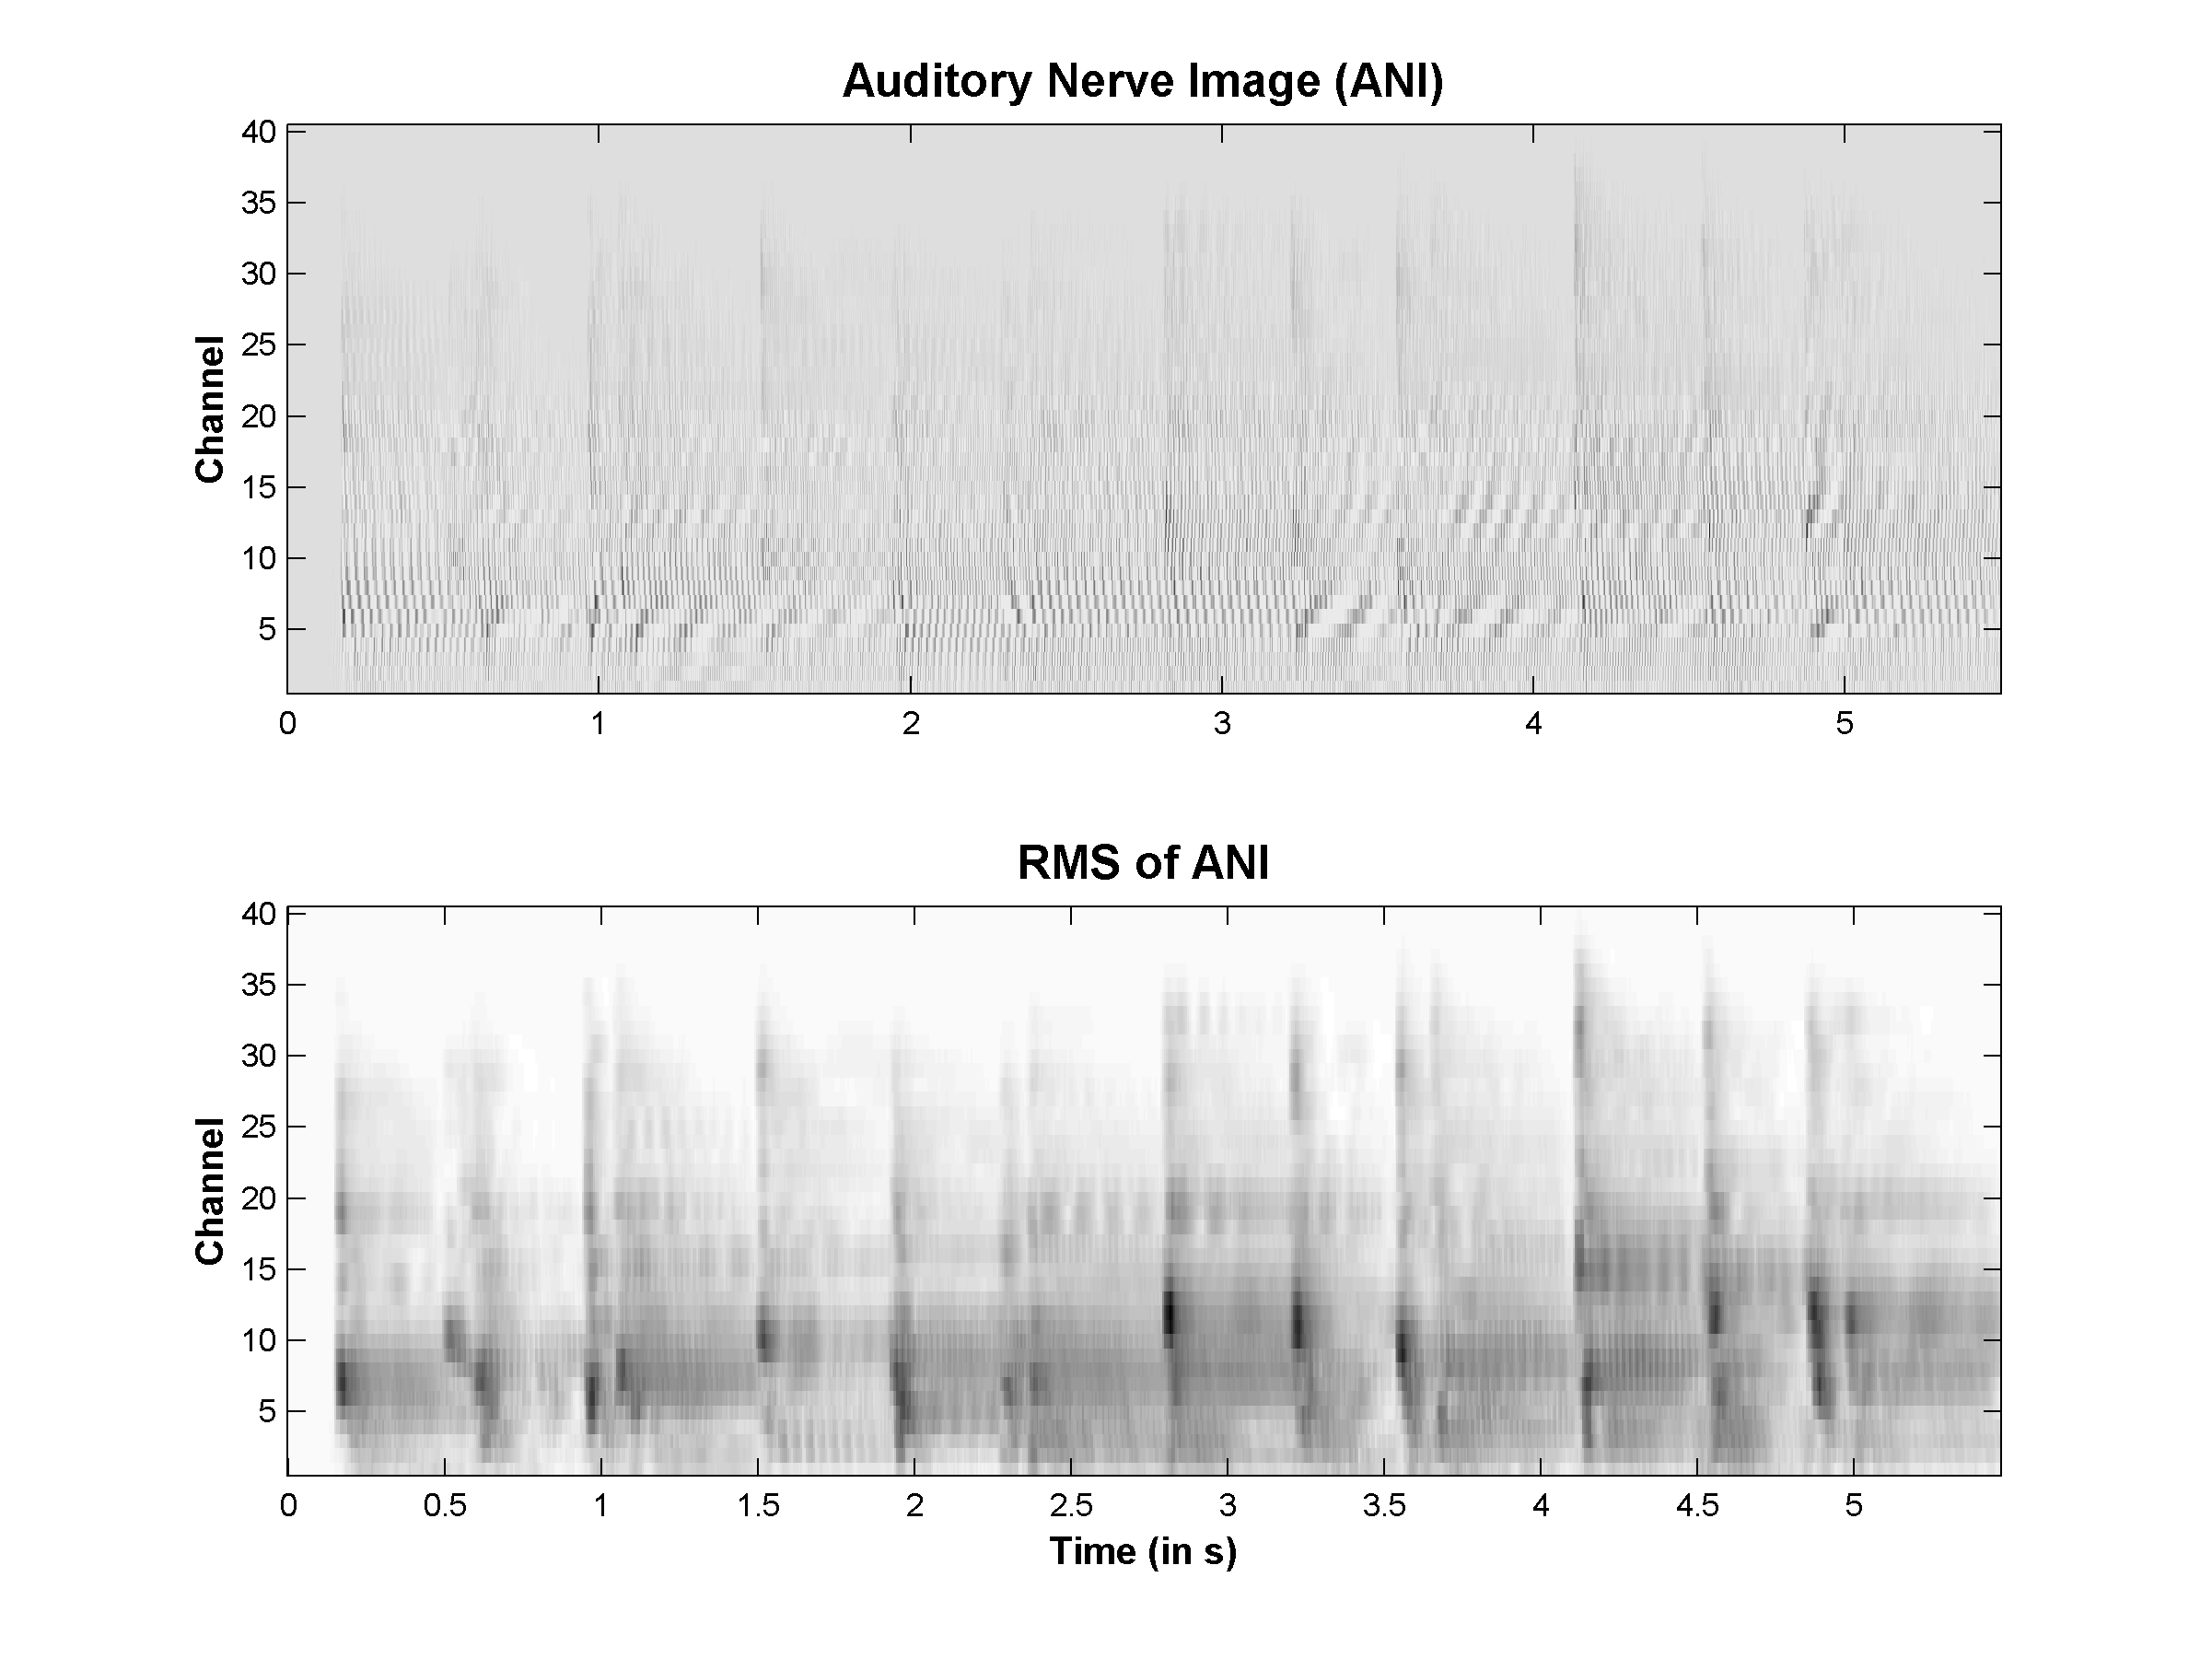
\includegraphics[width=\IPEMDefaultFigureWidth]{Graphics/OnsetsANIAndRMS}
    \caption{Top: ANI of the Schumann sound excerpt. Bottom: RMS values of the ANI.}
    \label{Fig:OnsetsANIAndRMS}
\end{figure}

\begin{figure}[h]
    \centering
    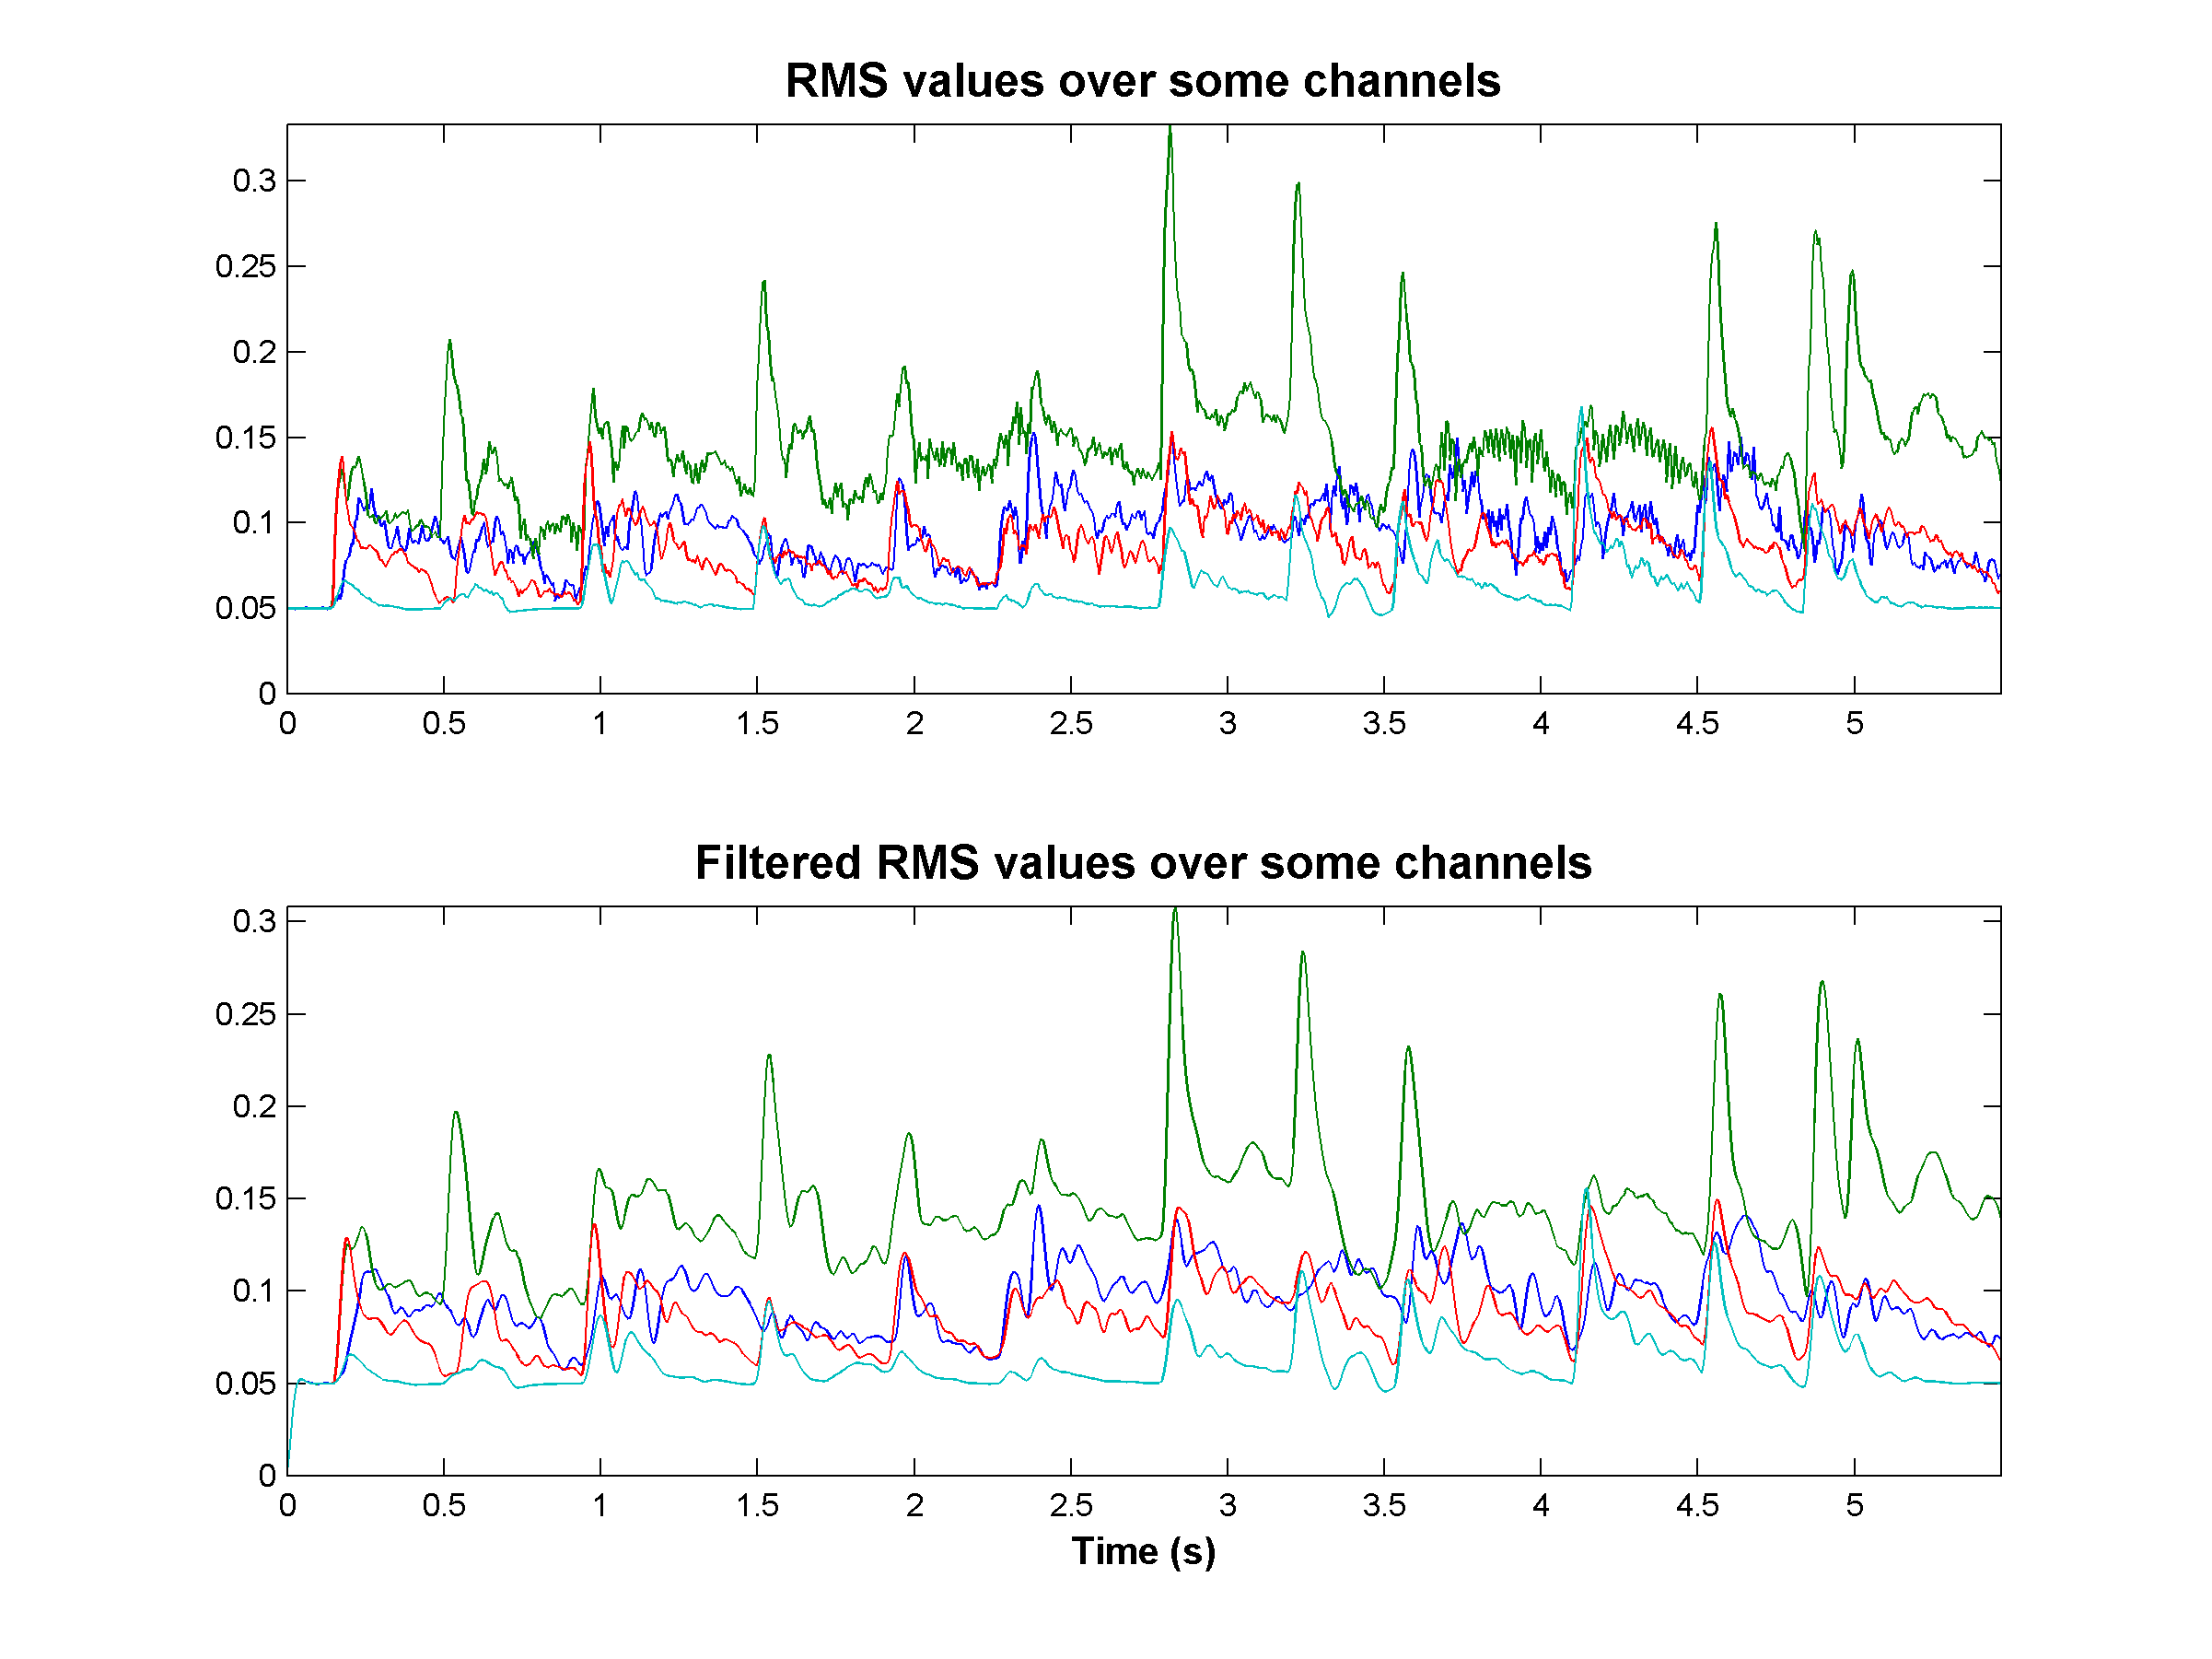
\includegraphics[width=\IPEMDefaultFigureWidth]{Graphics/OnsetsFilteredRMS}
    \caption{Top: RMS values for some channels of the ANI. Bottom: low pass filtered RMS values for the same channels.}
    \label{Fig:OnsetsFilteredRMS}
\end{figure}

\begin{figure}[h]
    \centering
    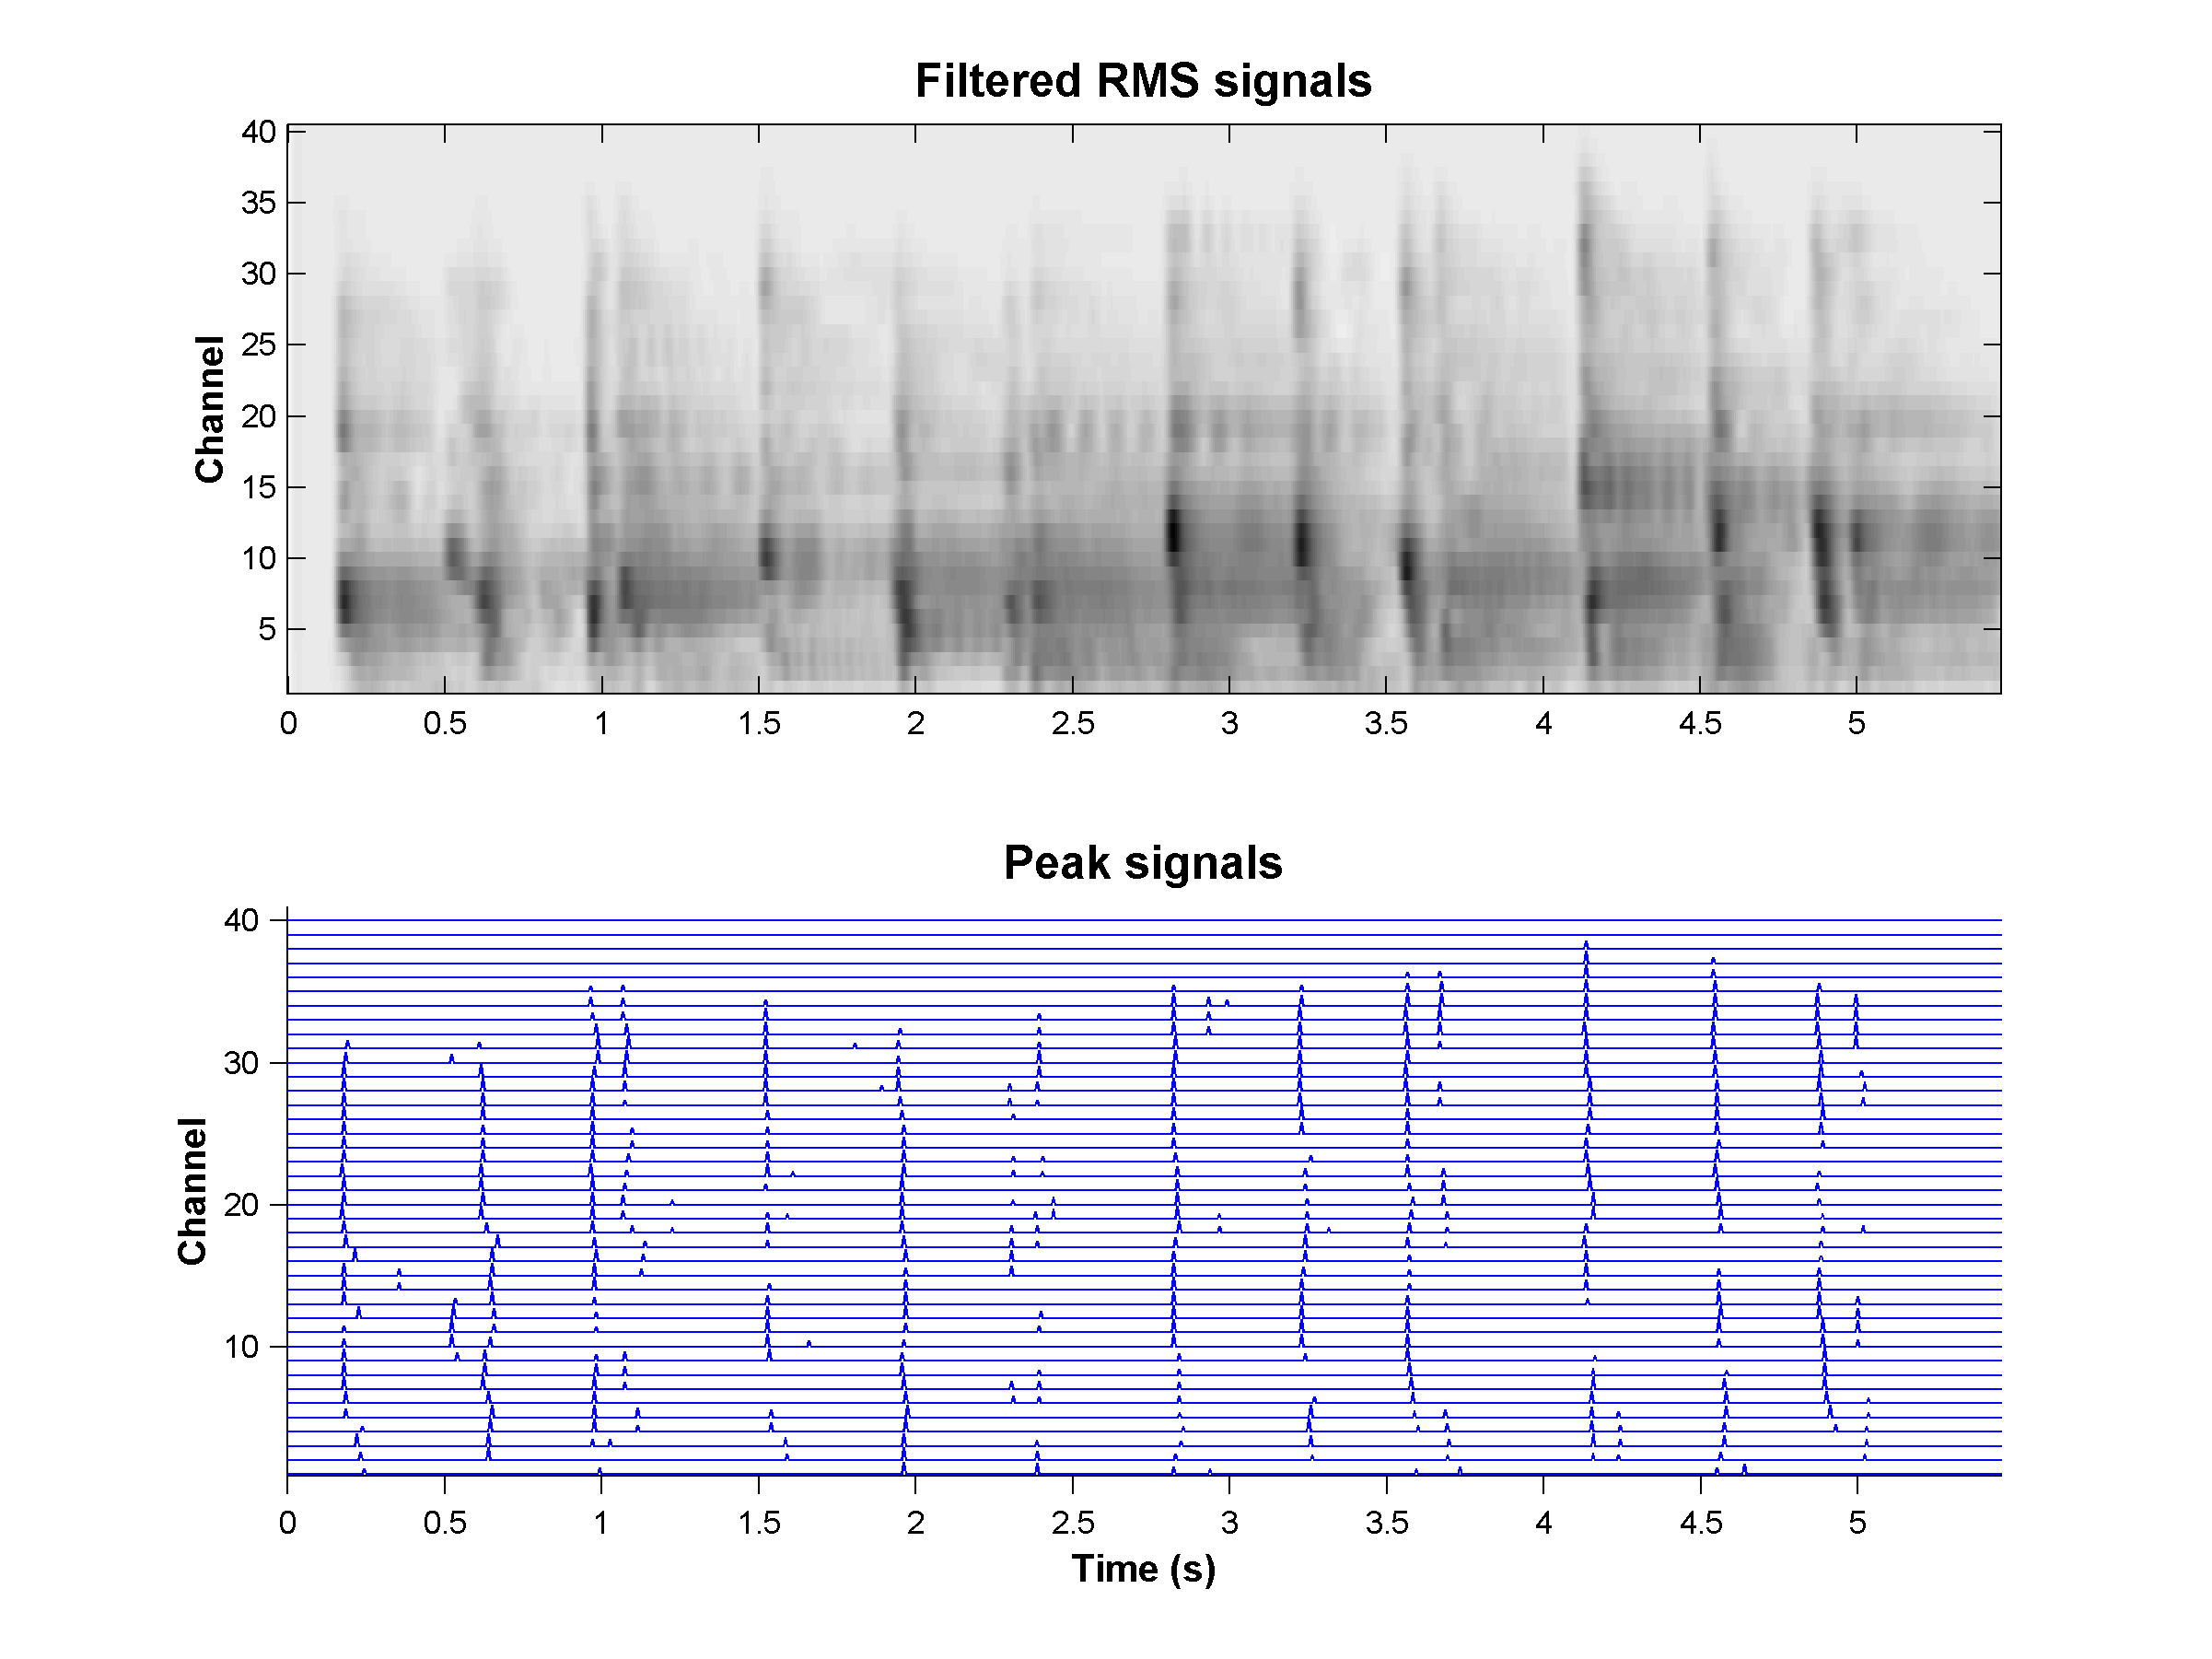
\includegraphics[width=\IPEMDefaultFigureWidth]{Graphics/OnsetsOnsetPeakDetection}
    \caption{Top: filtered RMS values of the ANI. Bottom: peaks detected for each channel.}
    \label{Fig:OnsetsOnsetPeakDetection}
\end{figure}

\begin{figure}[h]
    \centering
    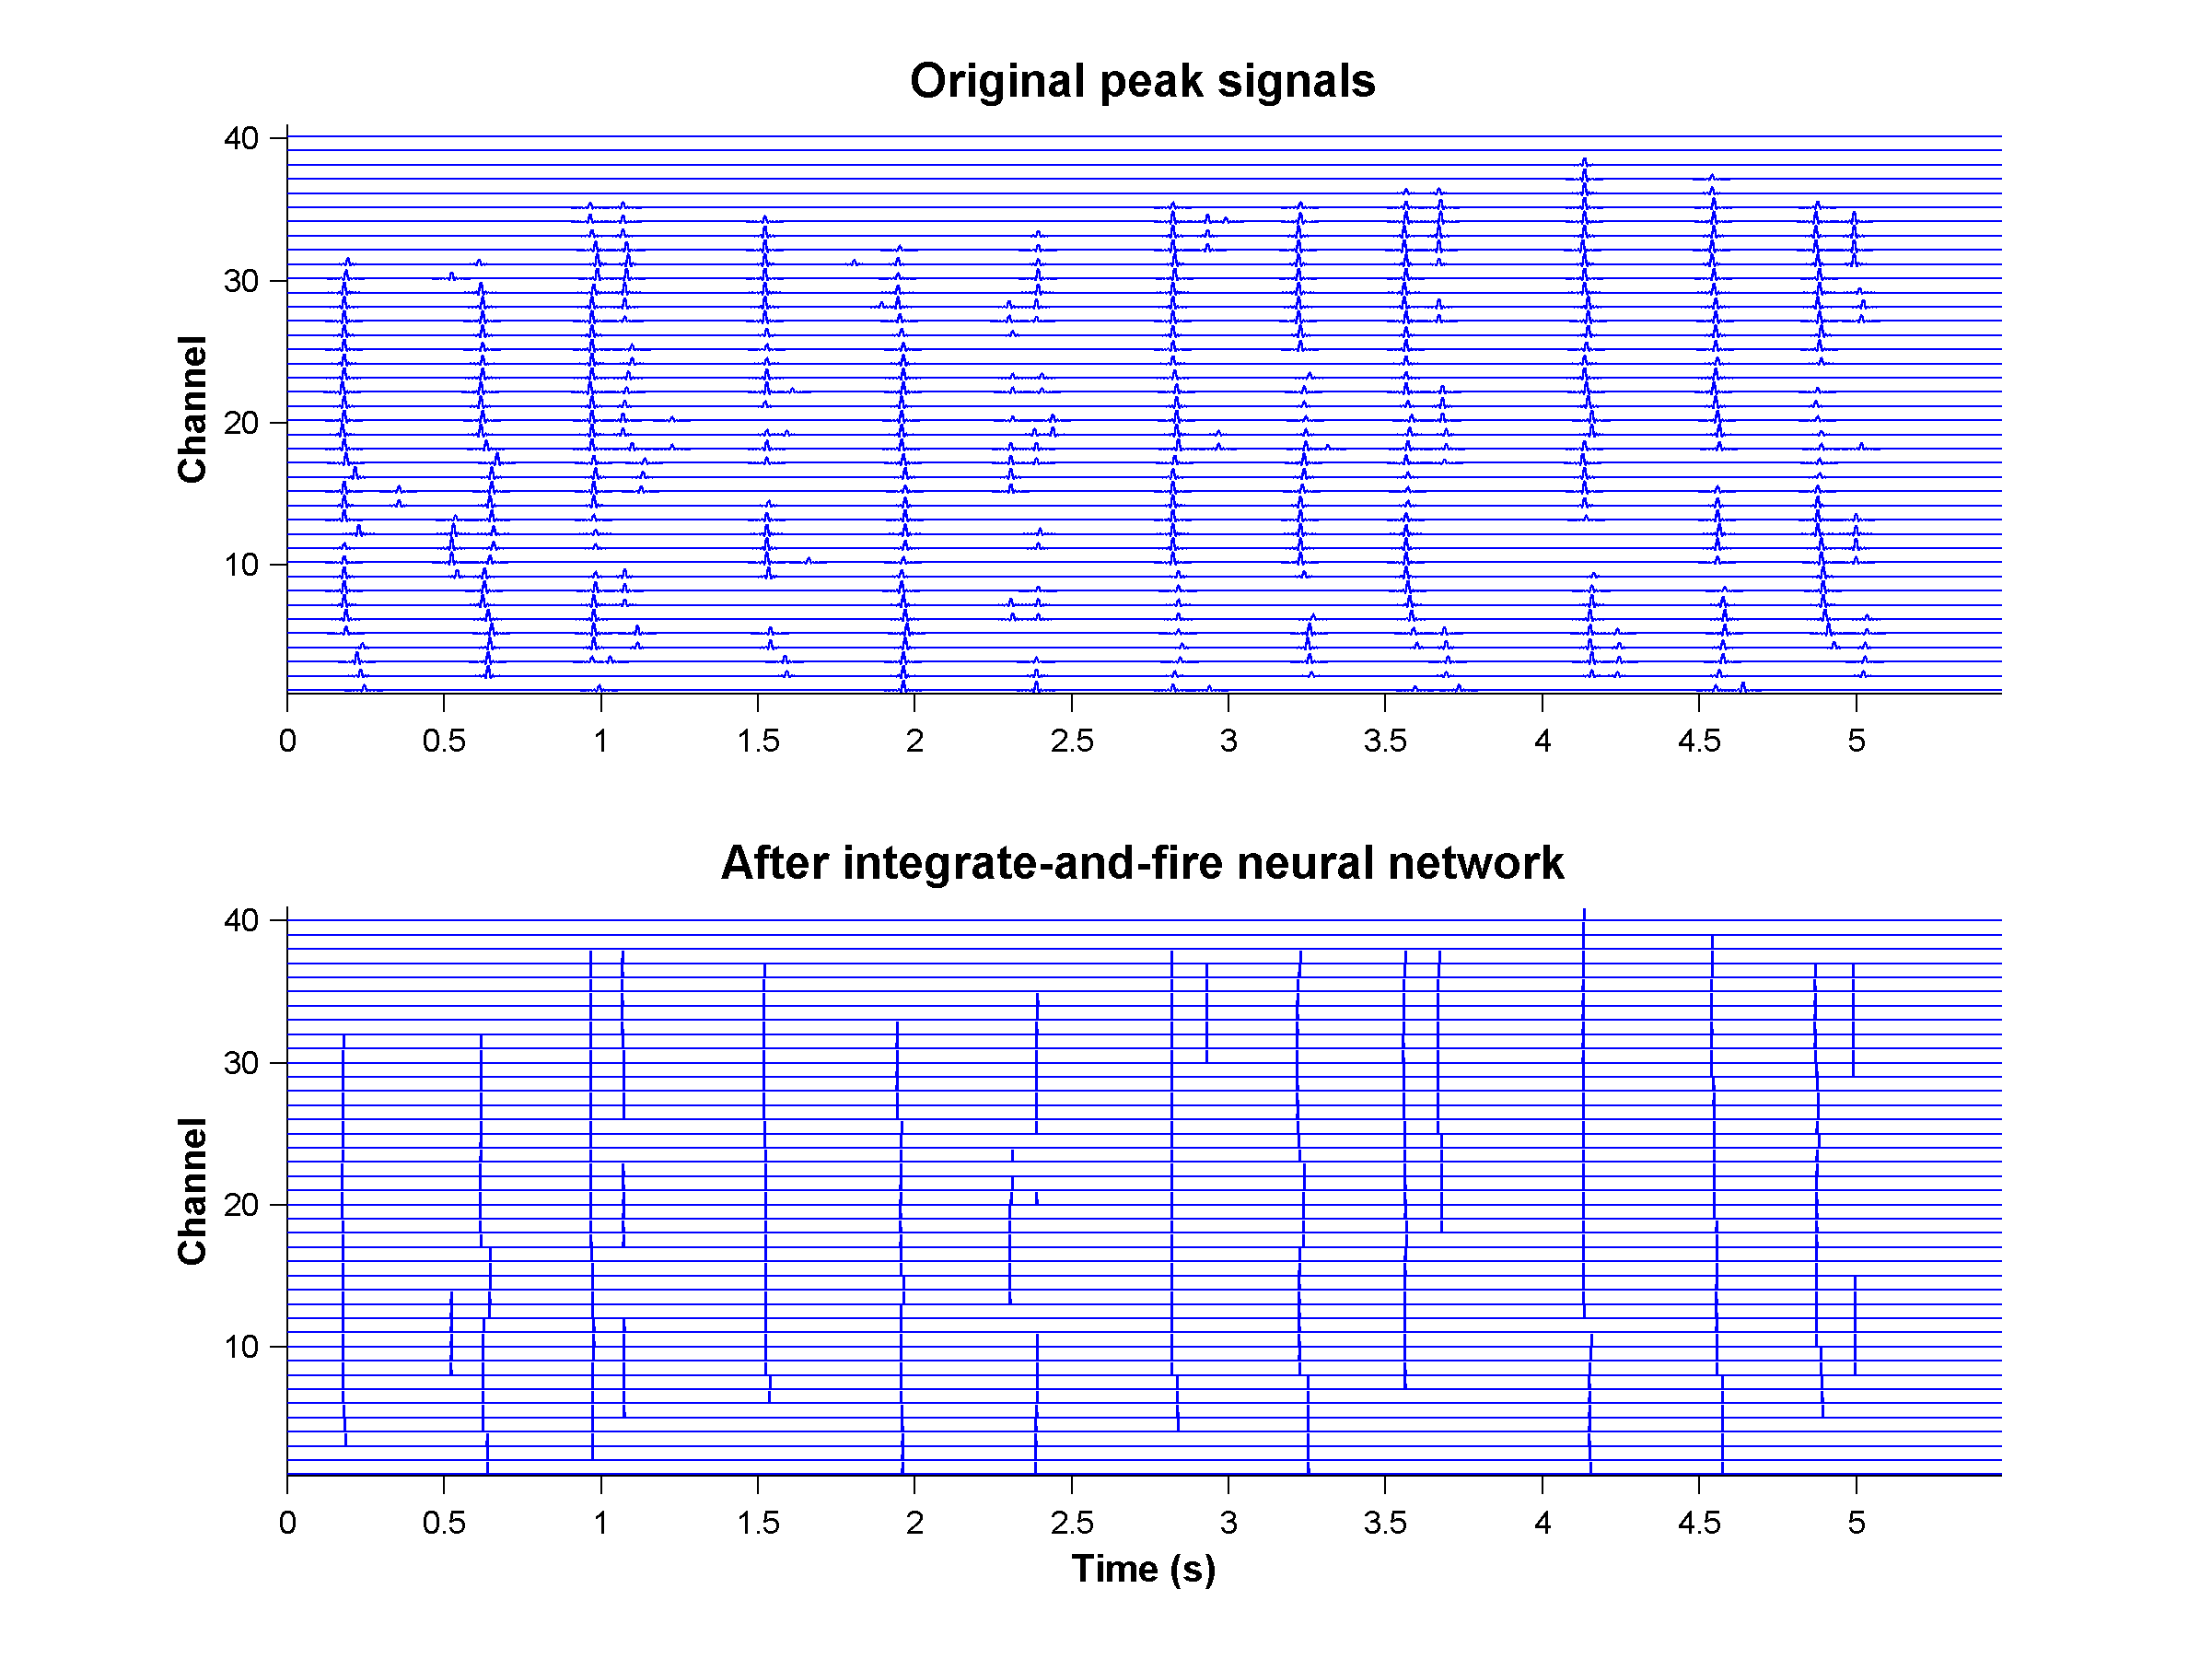
\includegraphics[width=\IPEMDefaultFigureWidth]{Graphics/OnsetsOnsetPattern}
    \caption{Top: detected peaks. Bottom: peaks after applying the integrate-and-fire neural network.}
    \label{Fig:OnsetsOnsetPattern}
\end{figure}

\begin{figure}[h]
    \centering
    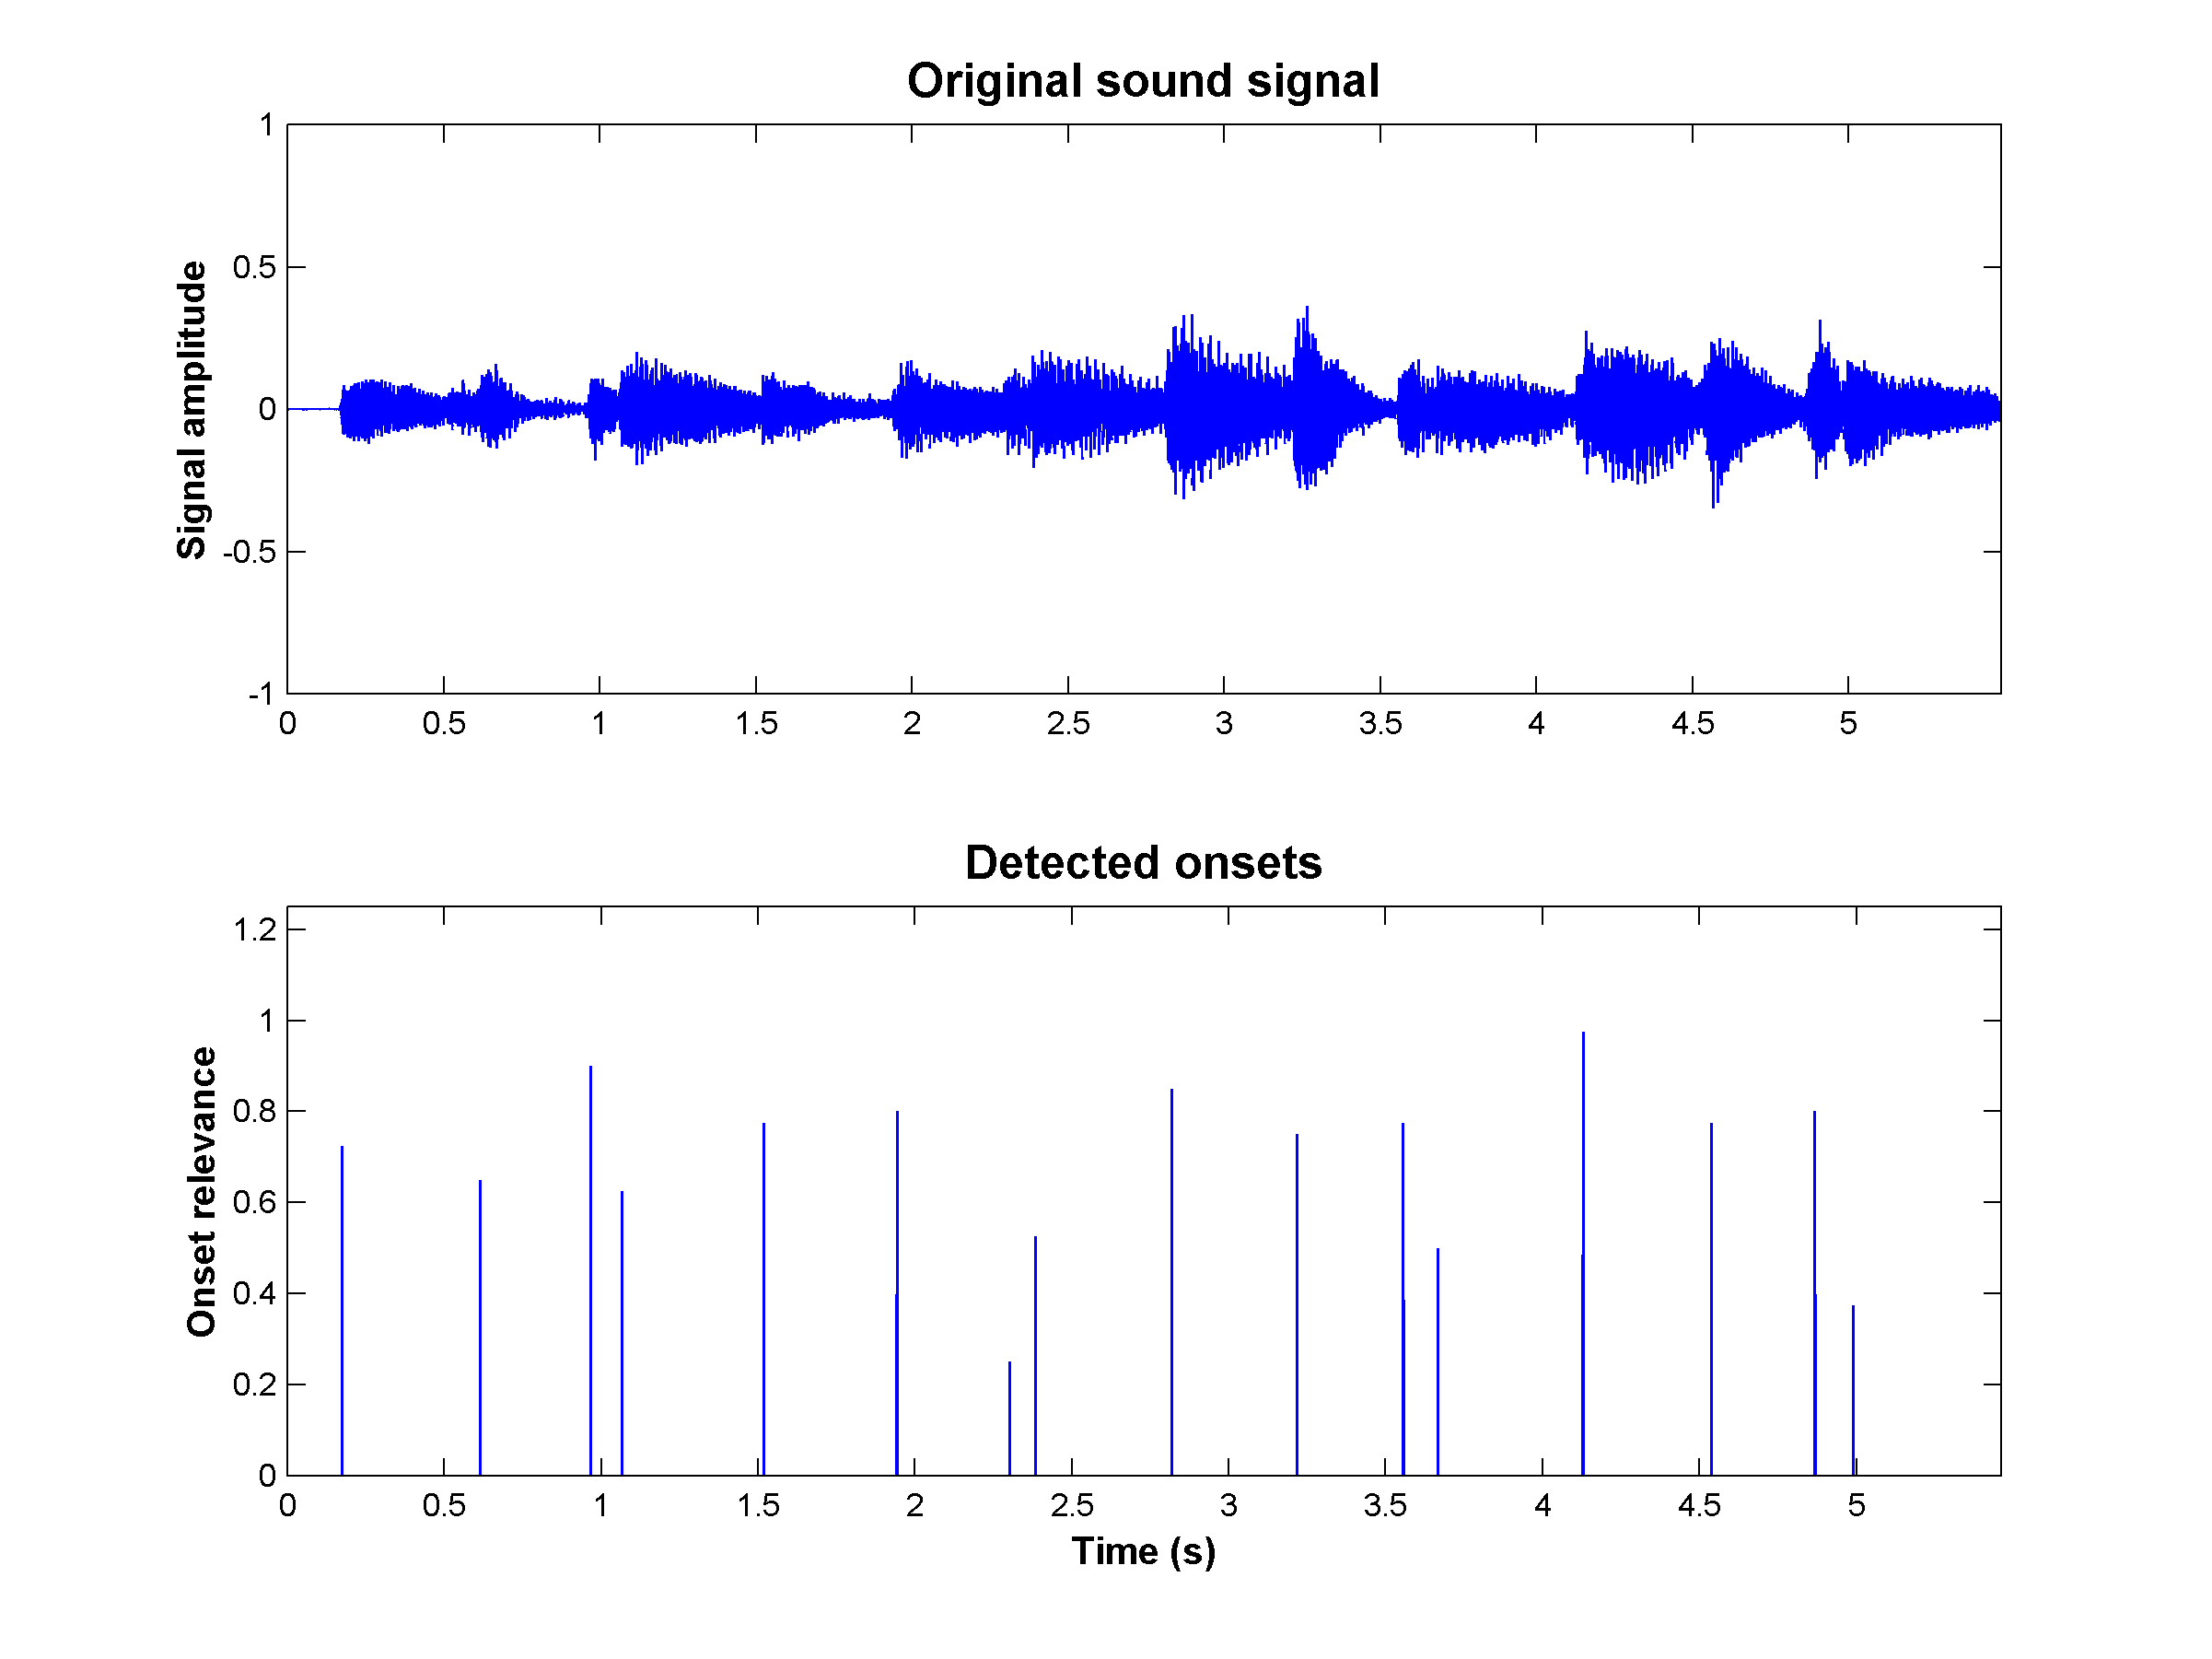
\includegraphics[width=\IPEMDefaultFigureWidth]{Graphics/OnsetsOnsetFilter}
    \caption{Top: original sound signal. Bottom: detected onsets and their relevance level.}
    \label{Fig:OnsetsOnsetFilter}
\end{figure}

\begin{figure}[h]
    \centering
    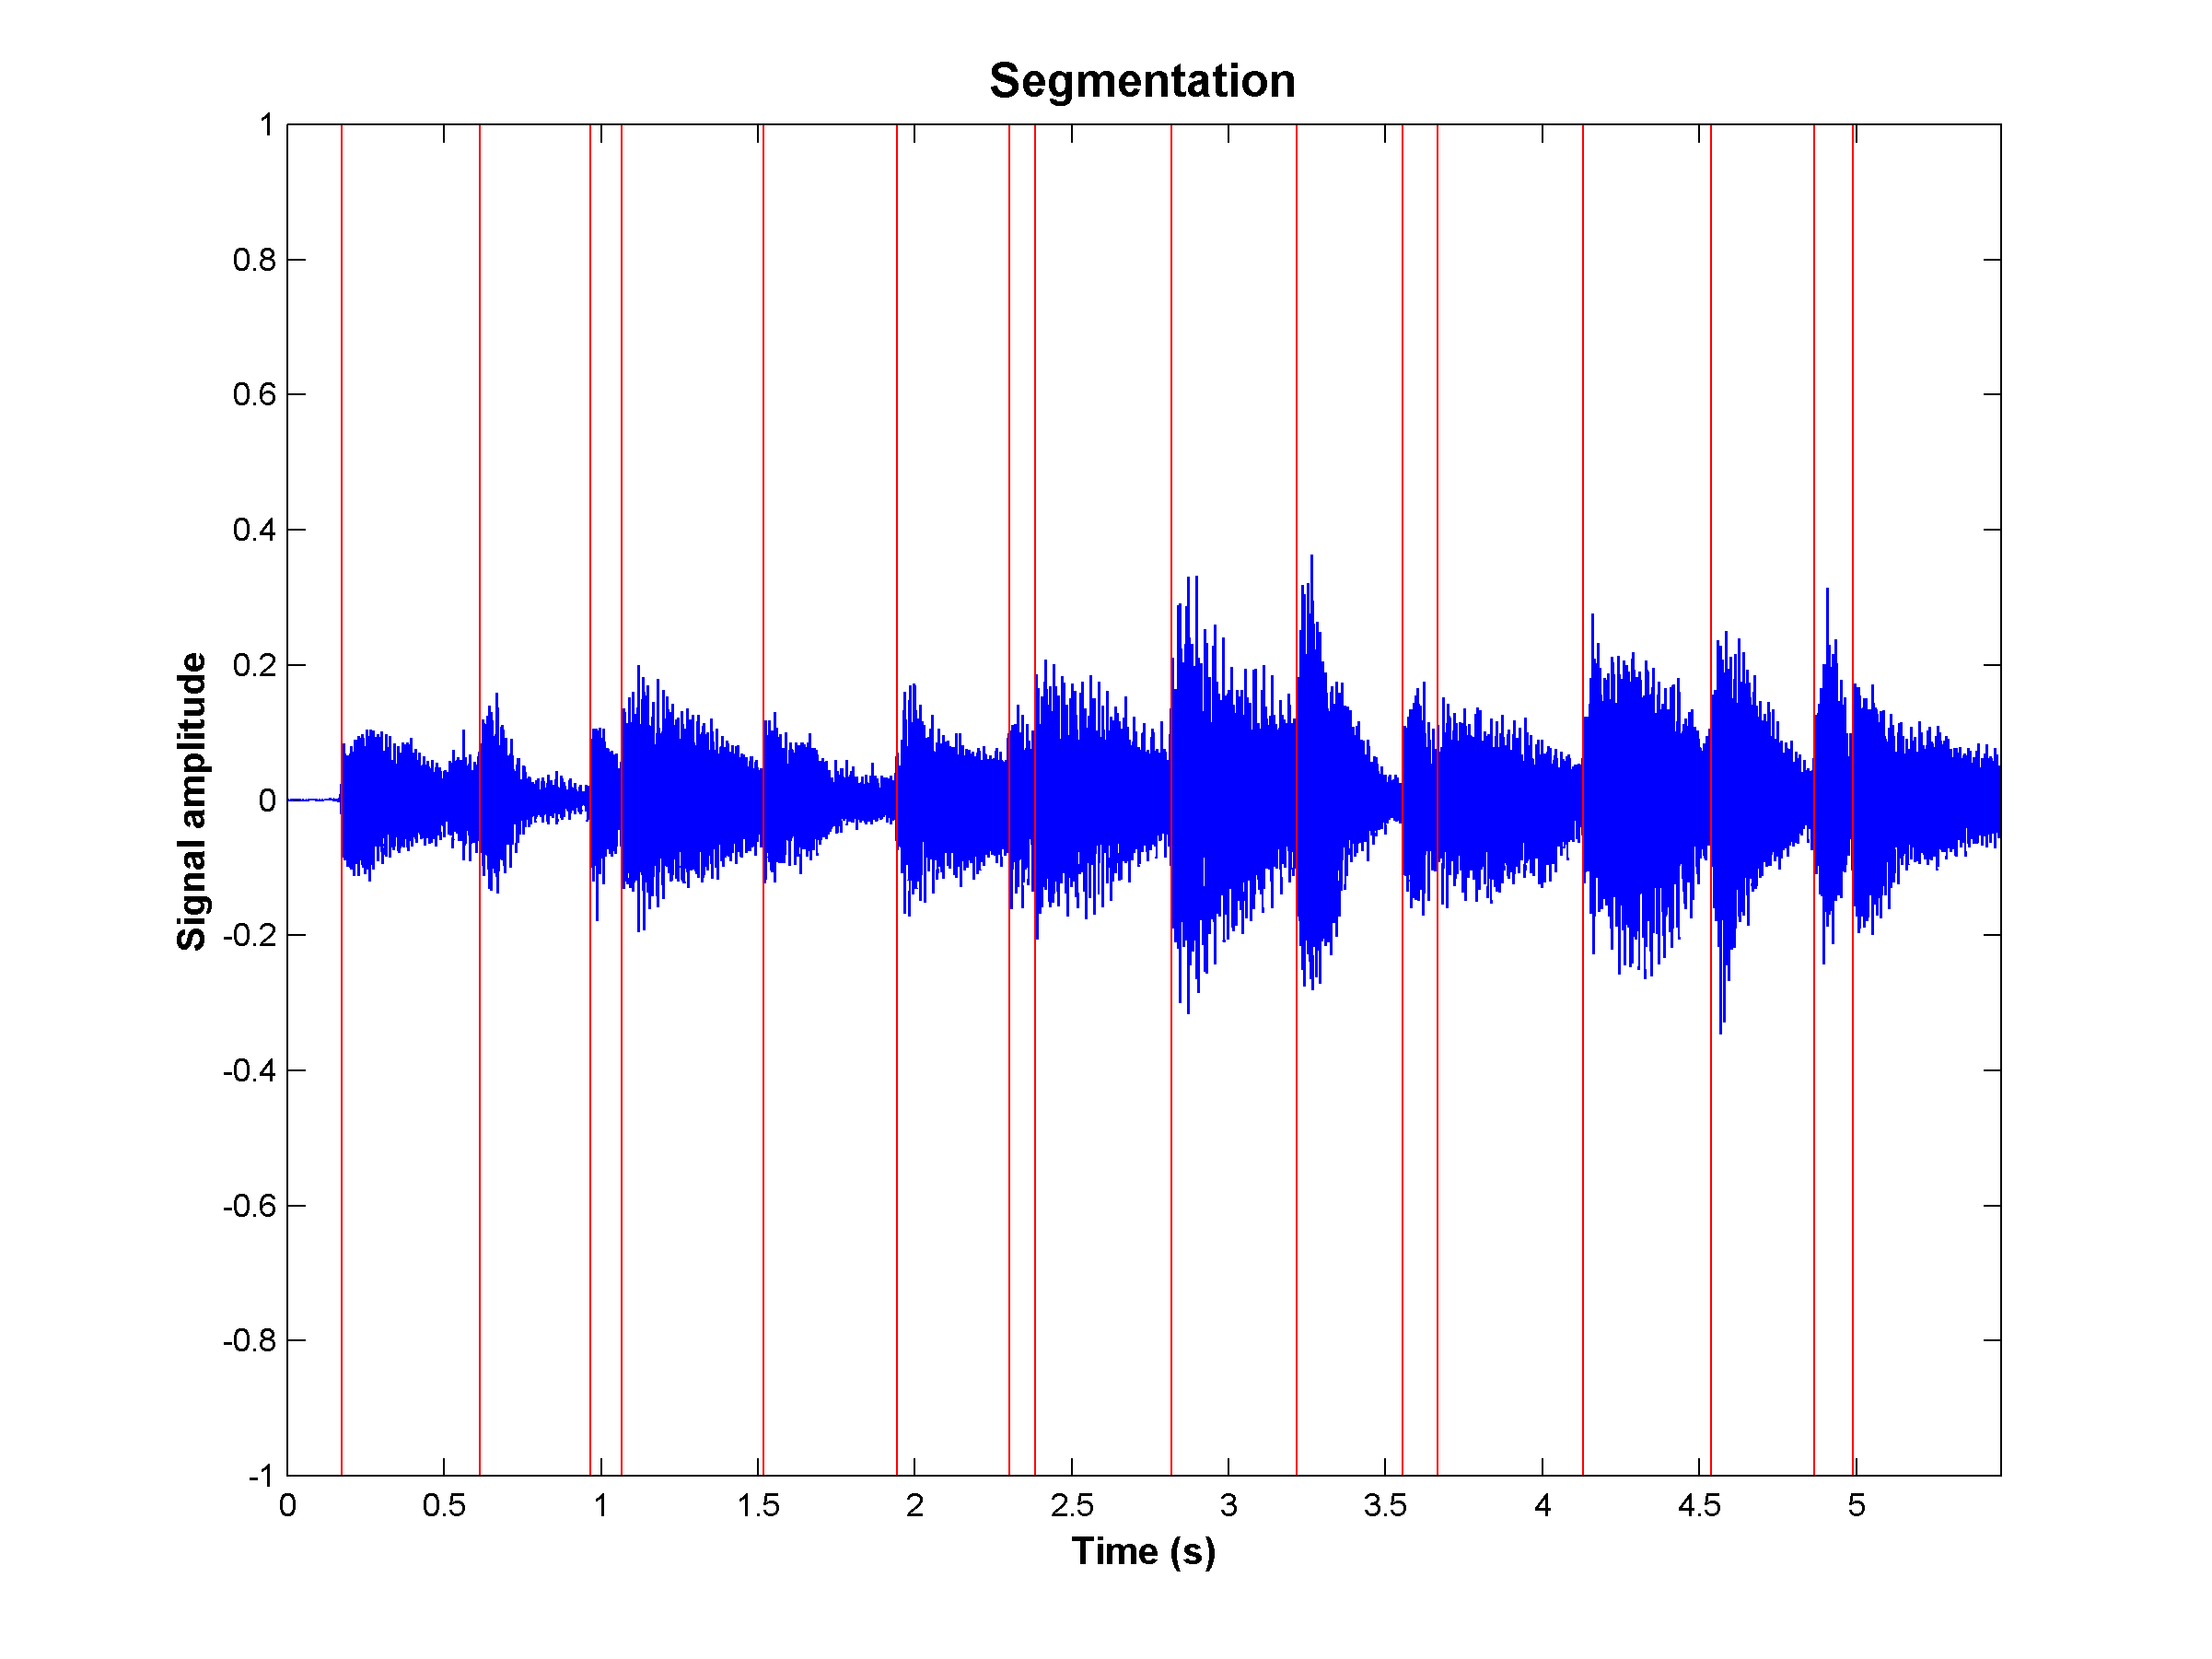
\includegraphics[width=\IPEMDefaultFigureWidth]{Graphics/OnsetsSegmentation}
    \caption{Segmentation of the original sound signal using the onset module.}
    \label{Fig:OnsetsSegmentation}
\end{figure}

% --------------------------------------------------------------------------------

% --------------------------------------------------------------------------------
% --------------------------------------------------------------------------------
\newpage
\section{Pitch Completion Module}
% --------------------------------------------------------------------------------

% Make general target
\hypertarget{Concepts:PitchCompletionModule}{}

% Make target for following functions:
\hypertarget{Concepts:IPEMPeriodicityPitch}{}

\subsection{Introductory description}
% --------------------------------------------------------------------------------

The Pitch Completion Module (PCM) calculates the periodicity pitch
image of a signal. Strictly speaking, the neural rate code of the
auditory nerve images is taken as input and a periodicity analysis
is the output. Otherwise stated, the inputs are primary images and
the outputs are pitch images. In our global chart of image
transformation modules PCM is localized in the section on
perception (fig. \ref{Fig:ModulesPCM}).
\begin{figure}[h]
    \centering
    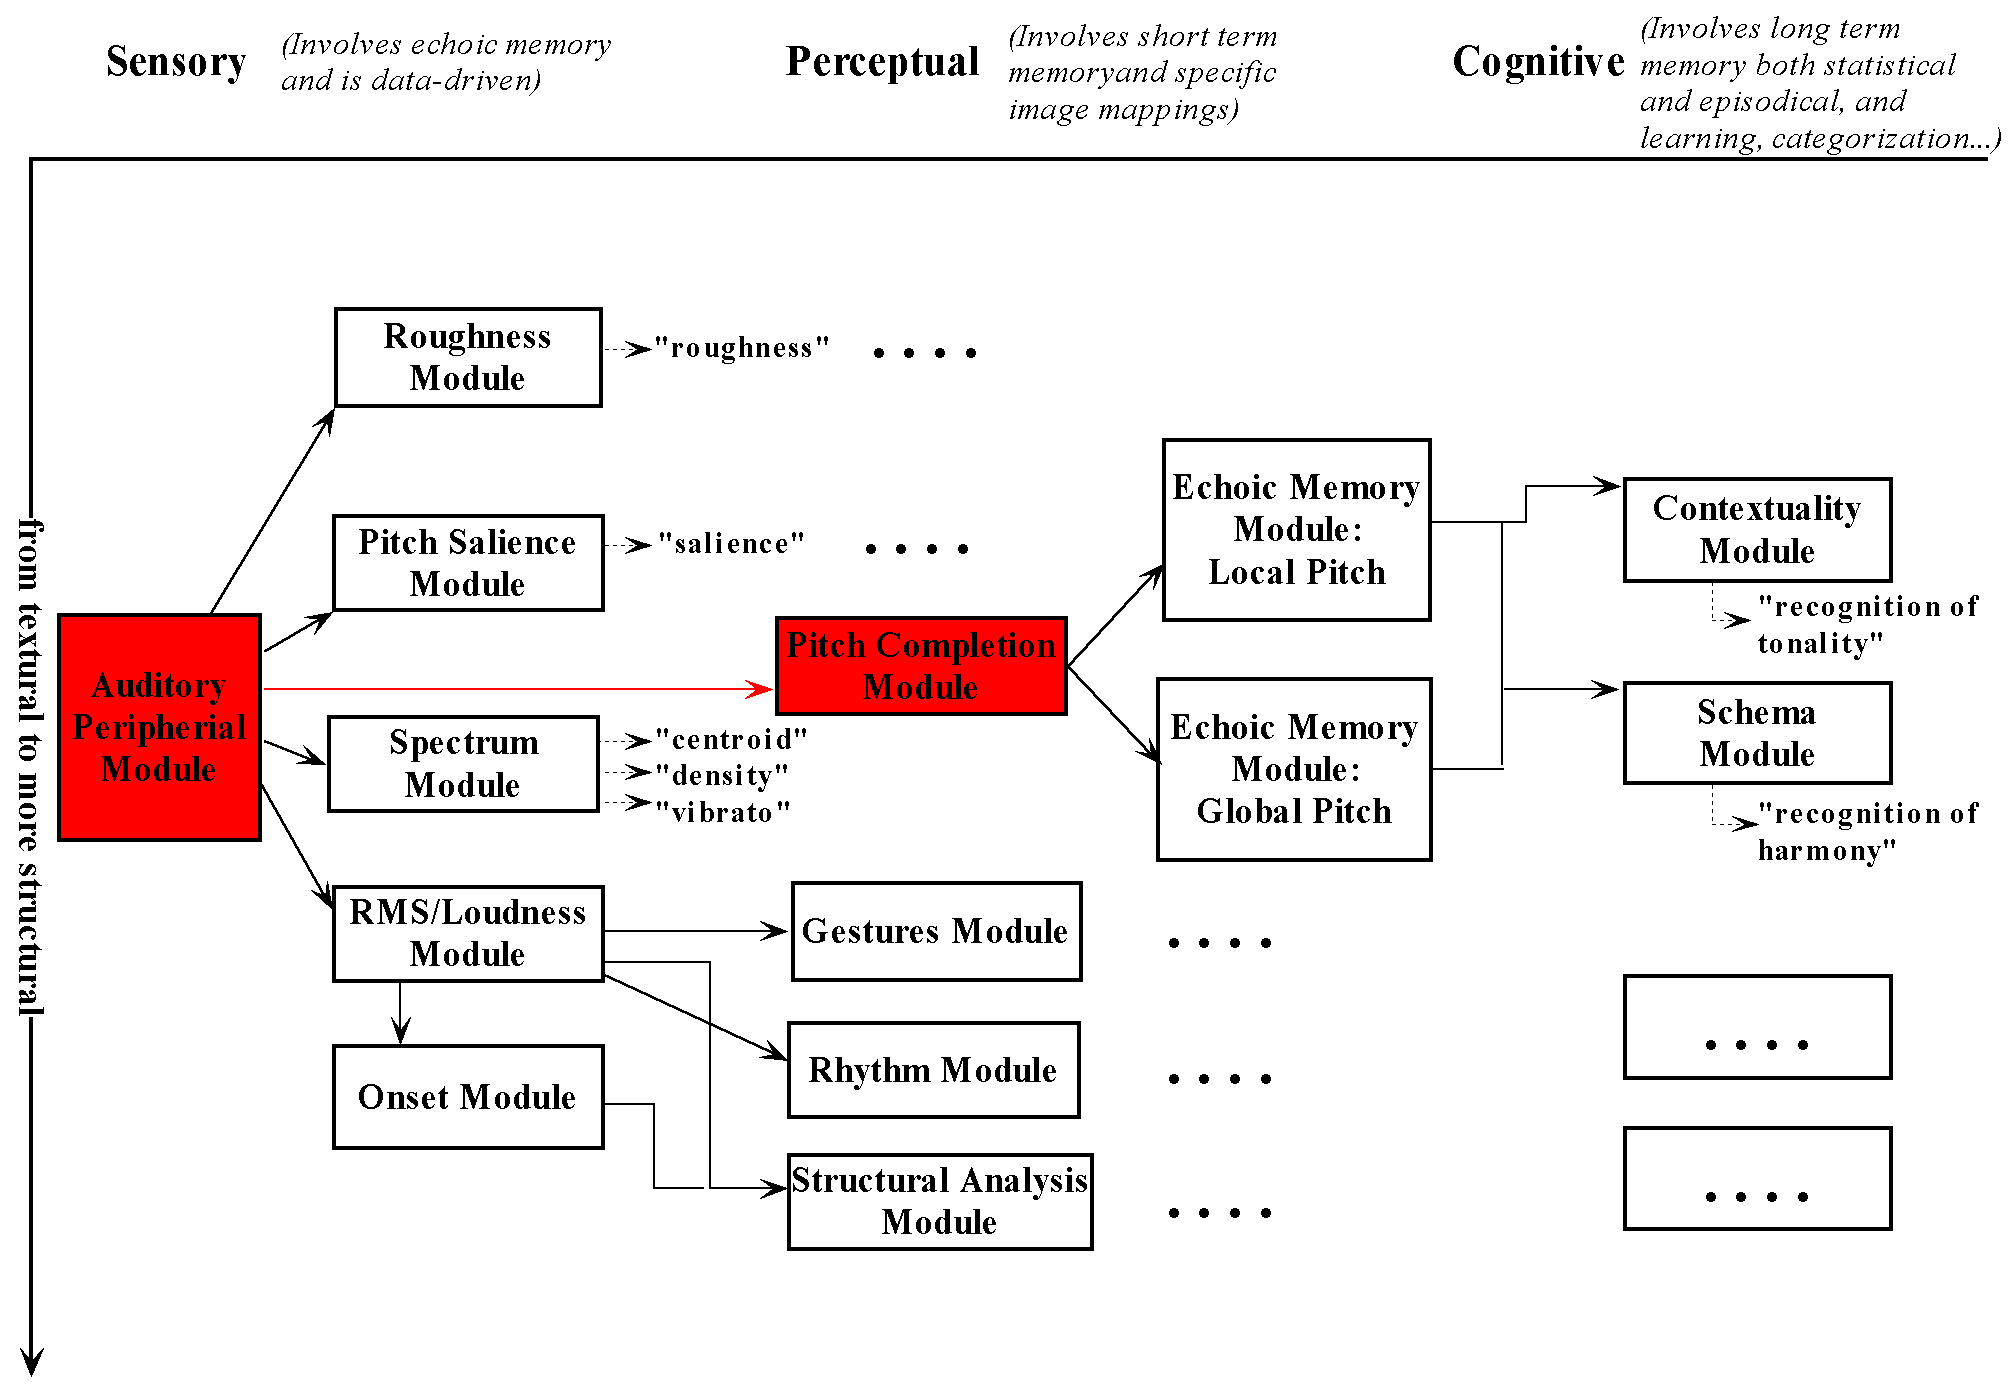
\includegraphics[width=\textwidth]{Graphics/ModulesPCM}
    \caption{Chart of image transformation modules, with PCM highlighted}
    \label{Fig:ModulesPCM}
\end{figure}

A periodicity analysis of primary images is dealt with at
different occasions, such as in
\hyperlink{Concepts:RhythmModule}{rhythm}. The main difference is
the focus of attention. In rhythm periodicity we look at larger
periodicities than in pitch where the focus of our attention is
between 80 and 1250 Hz.
\begin{itemize}
\item
    The lower limit of 80 Hz accounts for the fact that for smaller frequencies,
    the sensation of pitch becomes more a sensation of textural properties.
    This is a shift of perceptual categorization which is taken into account
    in our modeling. Indeed, our model of \hyperlink{Concepts:RoughnessModule}{roughness}
    took into account a range of frequencies between 5 and 300 Hz but
    the focus was on frequencies between 50 and 70 Hz (see the filter characteristics
    in figure \ref{Fig:Filters}).
\item
    The higher limit of 1250 Hz is related to the limits of neural synchronization.
    Beyond about 1250 Hz, the neurons are no longer able to follow the exact
    period of the signal very accurately, and periodicity pitch becomes unreliable.
\end{itemize}
Pitch estimations at higher frequencies could rely on spectral
information contained in $e(t,c)$. Such spectral images could be
obtained by taking the RMS-values in each channel over short time
periods using \hyperlink{FuncRef:IPEMCalcRMS}{IPEMCalcRMS}.
However, the pitch information necessary to deal with harmonic
relationships, is here assumed to be contained in the time-code of
the auditory nerve images, and this within a frequency band of 80
to 1250 Hz.

From a conceptual point of view the Pitch Completion Module
performs a transformation from time-code to place-code, i.e. from
patterns whose frequency is contained within the temporal
characteristics of the pattern to patterns whose frequency is
encoded along a spatial array. Physiological evidence for
periodicity pitch perception has been gathered by
\citeA{Langner:92,Langner:97}. Figure \ref{Fig:PCMModule} shows the
modules involved in the image transformation process.
\begin{figure}[h]
    \centering
    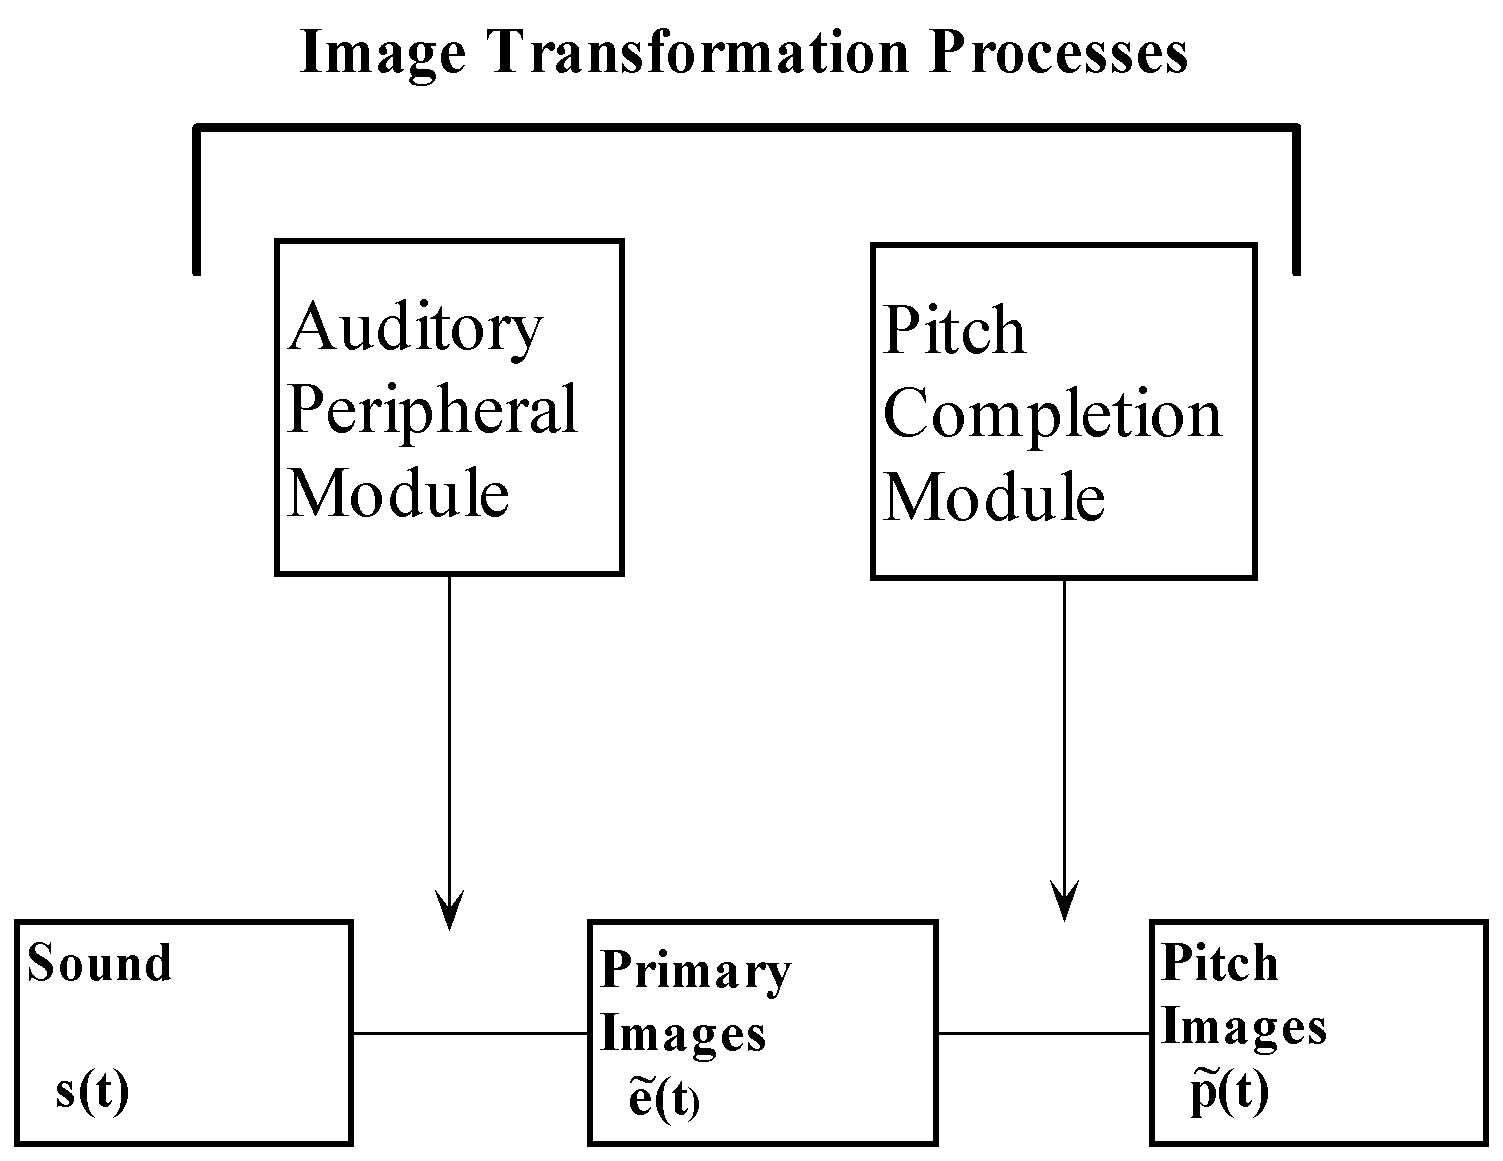
\includegraphics[width=\IPEMDefaultFigureWidth]{Graphics/PCMModule}
    \caption{Image Transformation Process: Pitch Completion Module}
    \label{Fig:PCMModule}
\end{figure}

\subsection{Functional-logical description}
% --------------------------------------------------------------------------------

First the auditory nerve images are calculated using the
\hyperlink{Concepts:AuditoryPeripheralModule}{Auditory Peripheral
Module}. The Pitch Completion Module then transforms these images
into pitch images.
\[APM:~ s(t) \rightarrow e(t,c)\]
\[PCM:~ e(t,c) \rightarrow p(t,\tau)~(=~\tilde{p}(t))\]

The Pitch Completion Module has two stages. First a periodicity
analysis of each $e(t,c)$ pattern, band-pass filtered for 80-1250
Hz, is made, where $f[e(t,c)]$ is the band-pass filtered auditory
nerve pattern for channel $c$, and $p(t,c,\tau)$ or
$\tilde{p}(t,c)$ the periodicity analysis of that pattern, with
$\tau$ denoting the period. The detected periods are registered
along a spatial array of periods. We thus have:
\begin{displaymath}
PCM1:~ \left[
\begin{array}{l}
f[e(t,1)] \\ f[e(t,2)] \\ \cdots \\ f[e(t,C)]
\end{array}
\right] \rightarrow \left[
\begin{array}{l}
\tilde{p}(t,1) \\ \tilde{p}(t,2) \\ \cdots \\ \tilde{p}(t,C)
\end{array}
\right]
\end{displaymath}

Secondly, a {\sl coincidence mechanism} sums up the
$\tilde{p}(t,c)$ over all channels patterns and stores the result
in a summary auto-correlation pattern called $\tilde{p}(t)$:
\begin{displaymath}
PCM2:~ \left[
\begin{array}{l}
\tilde{p}(t,1) \\ \tilde{p}(t,2) \\ \cdots \\ \tilde{p}(t,C)
\end{array}
\right] \rightarrow \tilde{p}(t)
\end{displaymath}

The resulting pattern $\tilde{p}$ (in alternative notation
$p(\tau)$) at time $t$ is called the pitch image or {\sl
completion image} at time $t$. The pitch is represented along the
$\tau$ axis. The completion image is related to the notion of
virtual pitch pattern. It gives an account of the common
periodicity along the auditory neurons in the frequency region of
80 Hz to 1250 Hz. Notice than the procedure outlined for PCM is
very similar to the procedure used for the detection of
periodicity in rhythm patterns, as described in the Example
section of the \hyperlink{Concepts:RhythmModule}{Rhythm Module}.

\subsection{Signal processing description}
% --------------------------------------------------------------------------------

These are the steps of the periodicity pitch calculation:

\begin{itemize}
\item Filtering\\
    The channels of the ANI are filtered between 80 and 1250 Hz. Due
    to the fact that the output of the auditory model gives the
    envelopes of the neural firing probabilities ($<$ 1250 Hz), it
    suffices to first apply a low-pass filter and then subtract that
    from the original signal in order to obtain the pitch. The
    low-pass filter is a second order Butterworth filter with a
    cutoff frequency of 80 Hz.
    \[ \tilde{e}_{filt}(t) = f[\tilde{e}(t)] \]
\item Auto-correlation\\
    A frame-based auto-correlation analysis is performed on the
    filtered channels. A frame width $FW$ and step size $FS$ are
    chosen and then for each frame and each channel $c$, we perform
    an auto-correlation for each time-lag $\delta$:
    \[
        p(t,c,\delta) = \int_{t}^{t+FW}{e_{filt,c}(\tau).e_{filt,c}(\tau+\delta).d\tau}
        \qquad \textrm{where $\delta \in [0,FW]$}
    \]
    and, by combining the results for all time lags $\delta$ in one
    vector, this gives us $\tilde{p}(t,c)$
\item Coincidence mechanism\\
    Summation of the auto-correlation results over all channels:
    \[ \tilde{p}(t) = \sum_{n=1}^{C}\tilde{p}(t,c) \]
\end{itemize}


\subsection{Implementation}
% --------------------------------------------------------------------------------

\begin{tabularx}{\linewidth}{llX}
\hyperlink{FuncRef:IPEMPeriodicityPitch}{IPEMPeriodicityPitch} & - & Calculates periodicity pitch from nerve image\\
\end{tabularx}


\subsection{Examples}
% --------------------------------------------------------------------------------

Figure \ref{Fig:SchumannPeriodicityPitch} shows the results of
first processing our familiar
\IPEMSound{Sounds/SchumannKurioseGeschichte.wav}{excerpt of
Schumann's Kuriose Geschichte} with the APM and then processing
the primary image with the Pitch Completion Module. The MATLAB
code is:\\

\begin{IPEMCodeEnvironment}
[ANI,ANIFreq,ANIFilterFreqs] = ...
\newline IPEMCalcANIFromFile('SchumannKurioseGeschichte.wav',[],[],1);
\newline [PP,PPFreq,PPPeriods,PPFANI] = IPEMPeriodicityPitch(ANI,ANIFreq,[],[],[],1);
\end{IPEMCodeEnvironment}\\

where \IPEMCodeExtract{PPFANI} are the filtered (between 80-1250
Hz) auditory nerve images.\\

Figure \ref{Fig:ShepardCChordPeriodicityPitch} shows the results
of first processing the \IPEMSound{Sounds/ShepardCChord.wav}{C
major chord using Shepard tones} with the APM and then processing
the primary image with the Pitch Completion Module.

\begin{figure}[h]
    \centering
    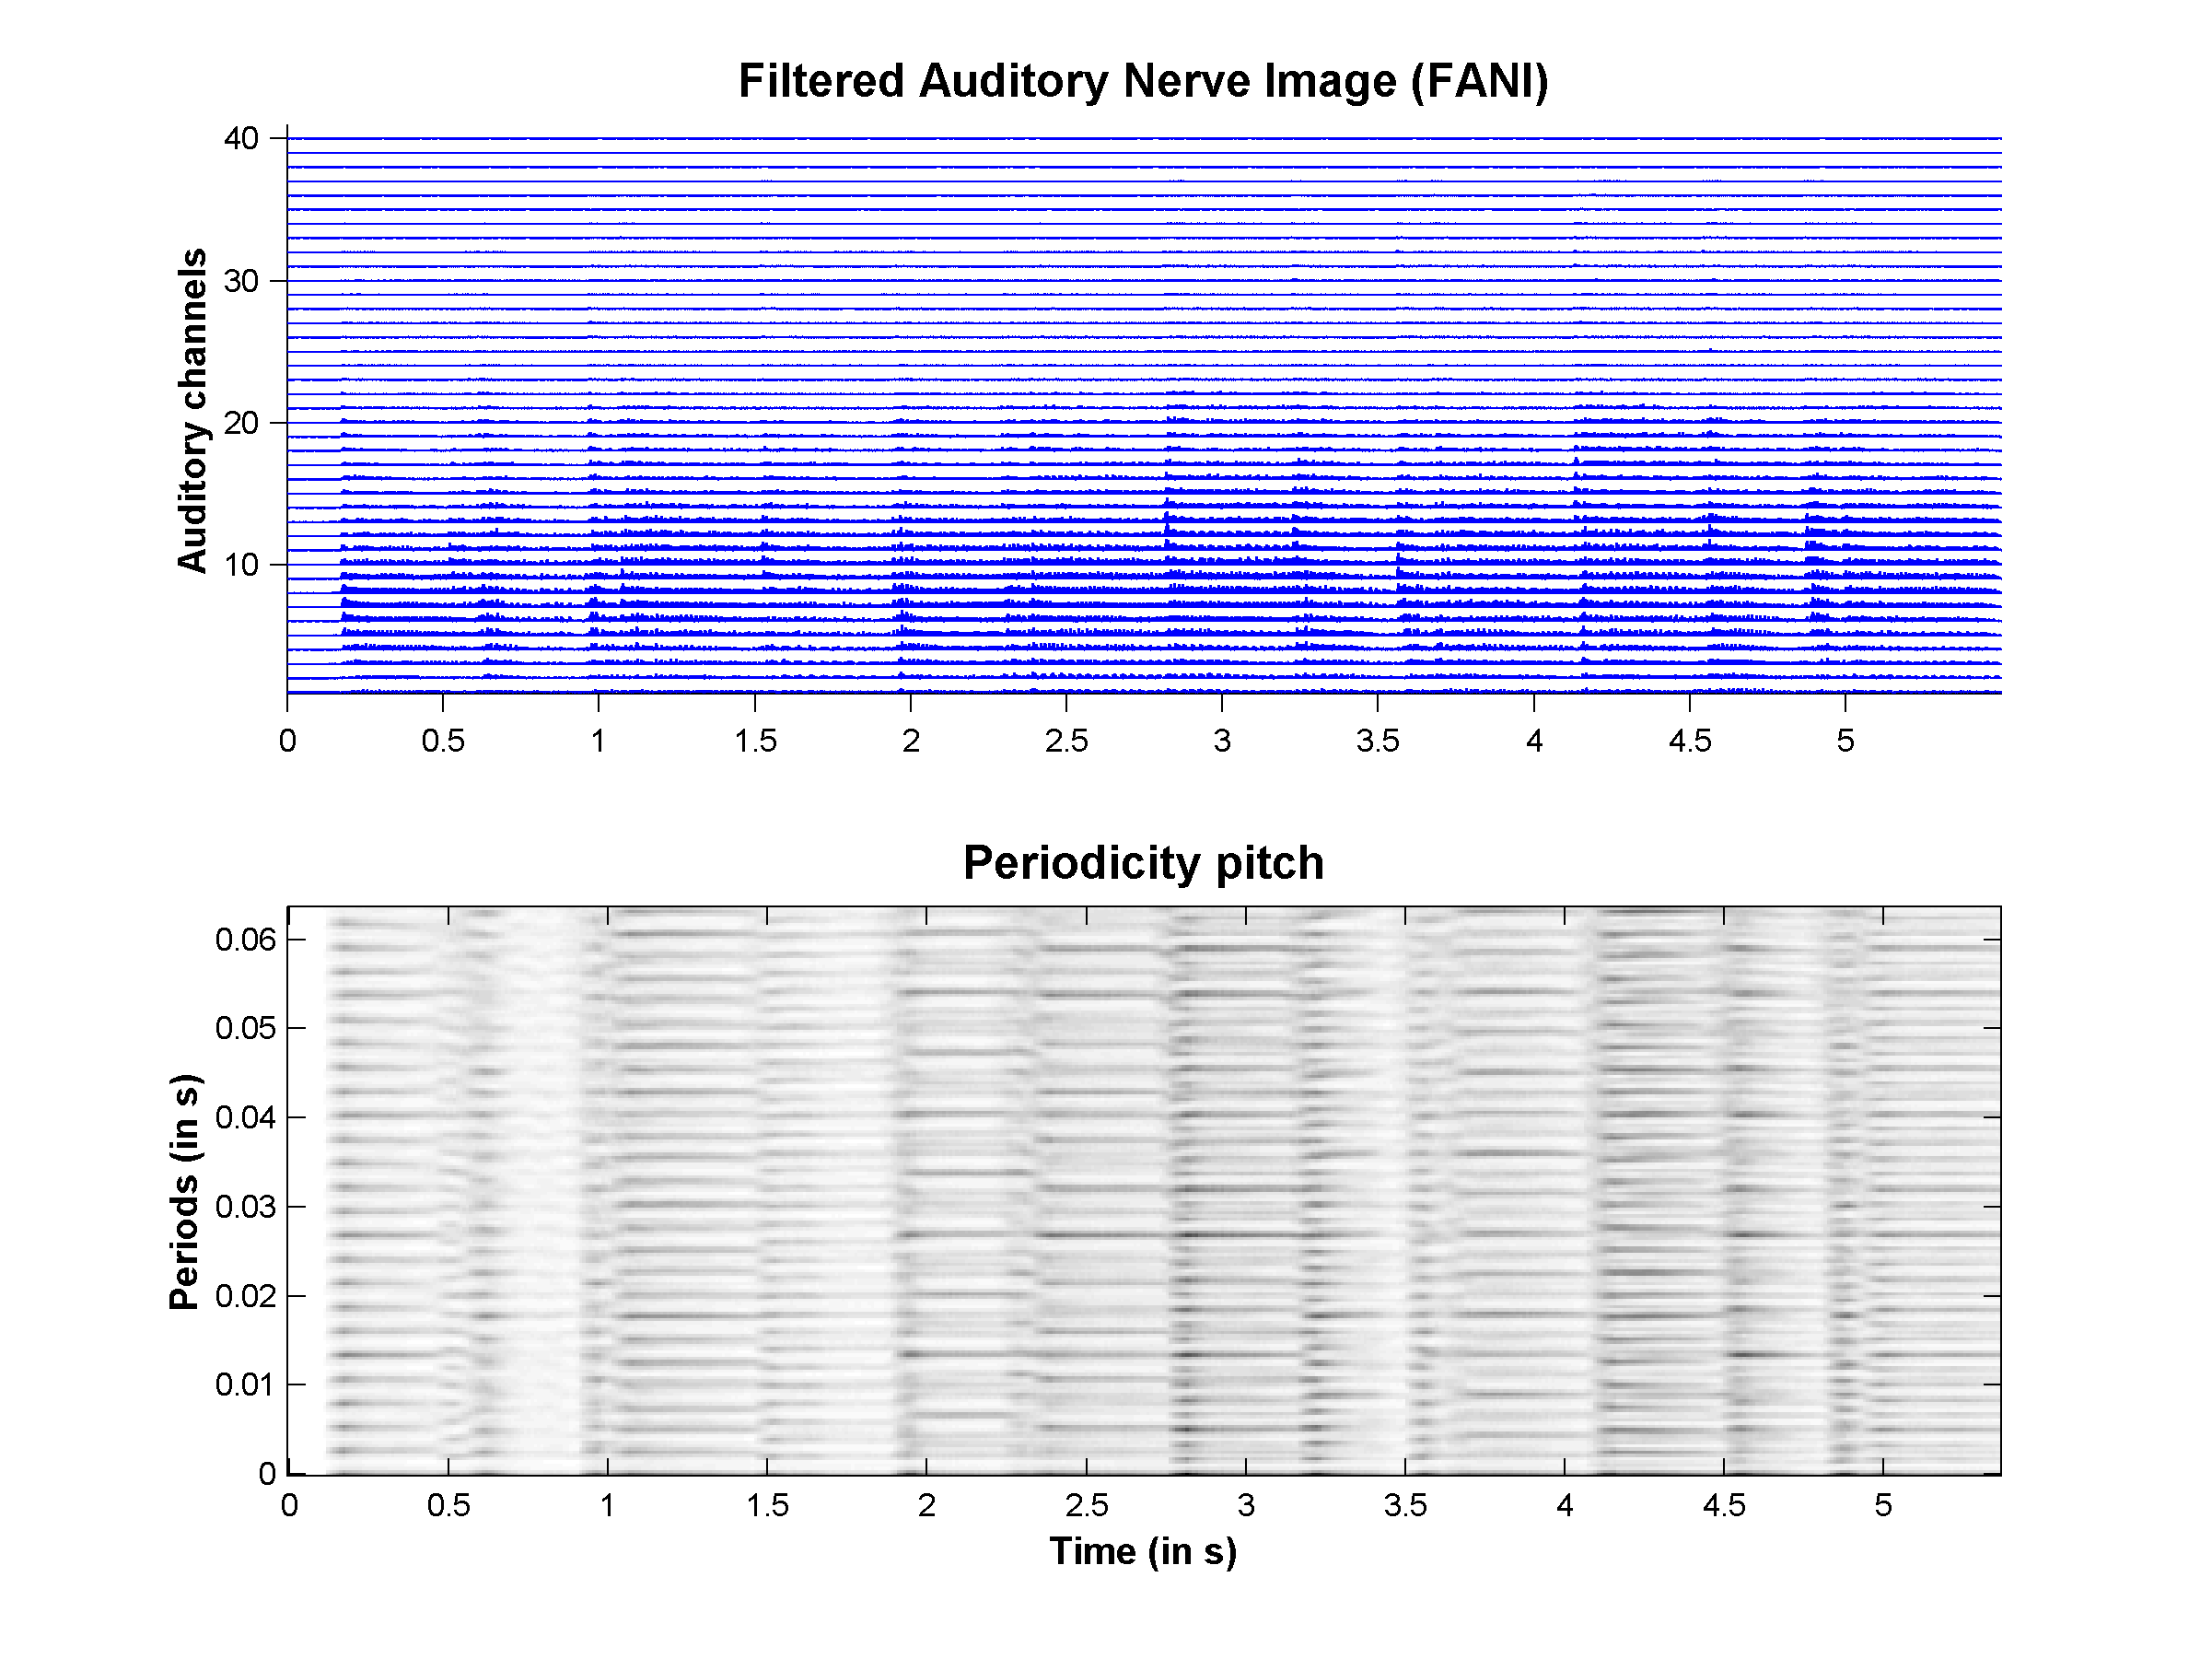
\includegraphics[width=\IPEMDefaultFigureWidth]{Graphics/SchumannPeriodicityPitch}
    \caption{Periodicity Pitch for the excerpt of Schumann's Kuriose Geschichte}
    \label{Fig:SchumannPeriodicityPitch}
\end{figure}

\begin{figure}[h]
    \centering
    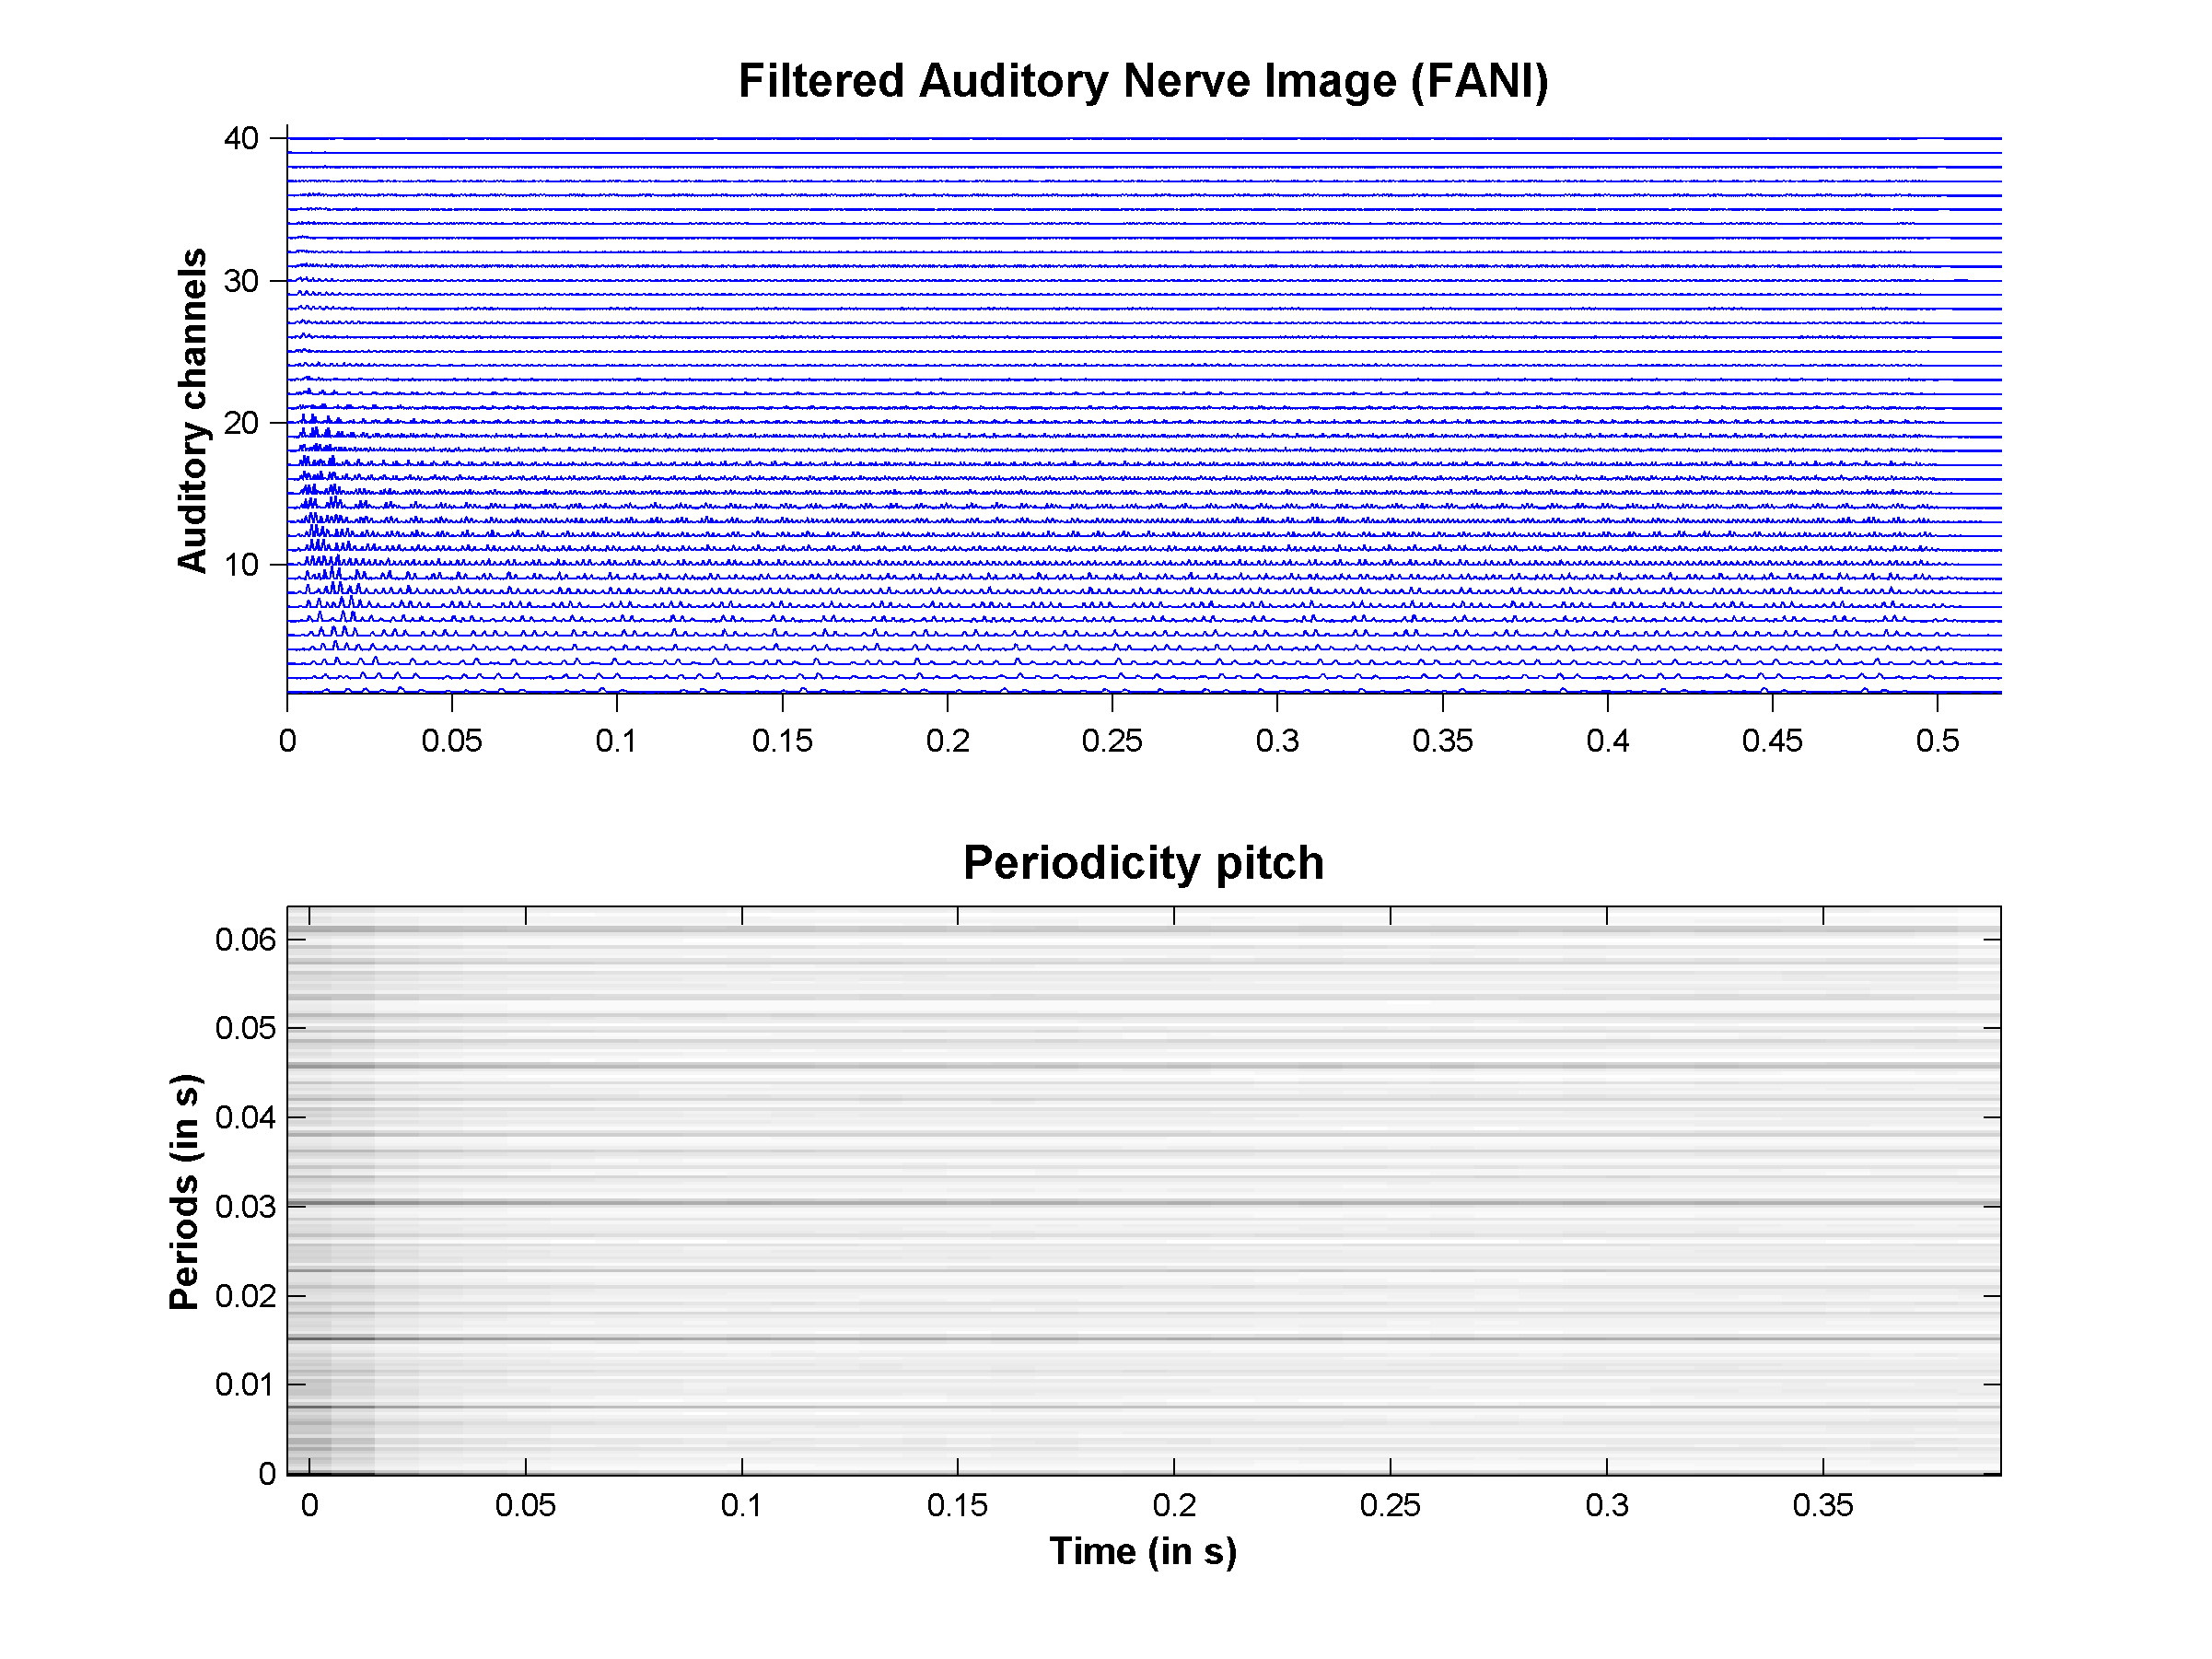
\includegraphics[width=\IPEMDefaultFigureWidth]{Graphics/ShepardCChordPeriodicityPitch}
    \caption{Periodicity Pitch for the C major chord using Shepard tones}
    \label{Fig:ShepardCChordPeriodicityPitch}
\end{figure}

% --------------------------------------------------------------------------------

% --------------------------------------------------------------------------------
% --------------------------------------------------------------------------------
\newpage
\section{Rhythm Module}
% --------------------------------------------------------------------------------

% Make general target
\hypertarget{Concepts:RhythmModule}{}

% Make target for following functions:
\hypertarget{Concepts:IPEMMECAnalysis}{}
\hypertarget{Concepts:IPEMMECExtractPatterns}{}
\hypertarget{Concepts:IPEMMECReSynthUI}{}
\hypertarget{Concepts:IPEMMECSynthesis}{}
\hypertarget{Concepts:IPEMMECSaveResults}{}

% Make target for normal references
\label{Concepts:RhythmModule}

\subsection{Introductory description}
% --------------------------------------------------------------------------------

The Rhythm Module (RhM) uses the Minimal Energy Change (MEC)
algorithm to calculate the fundamental period of a signal. The
input is a sound file and the output is an estimation of the
fundamental period at each time step. The technique used is a
generalization of the Average Magnitude Difference Function, known
as AMDF \cite{inproceedings:LemanVerbeke:Ieper:2000}. The basic
idea is that:
\begin{itemize}
\item
the energy calculated over the period of a repeating pattern is
more or less the same at each moment in time
\item
minimal changes of this energy point to the period of the
repetitive pattern.
\end{itemize}
In applying MEC to rhythm detection we perform the analysis on
the energy patterns in the auditory nerve images. This module
then has its place in the image transformation chart as shown in
figure \ref{Fig:ModulesRhM}.
\begin{figure}[h]
    \centering
    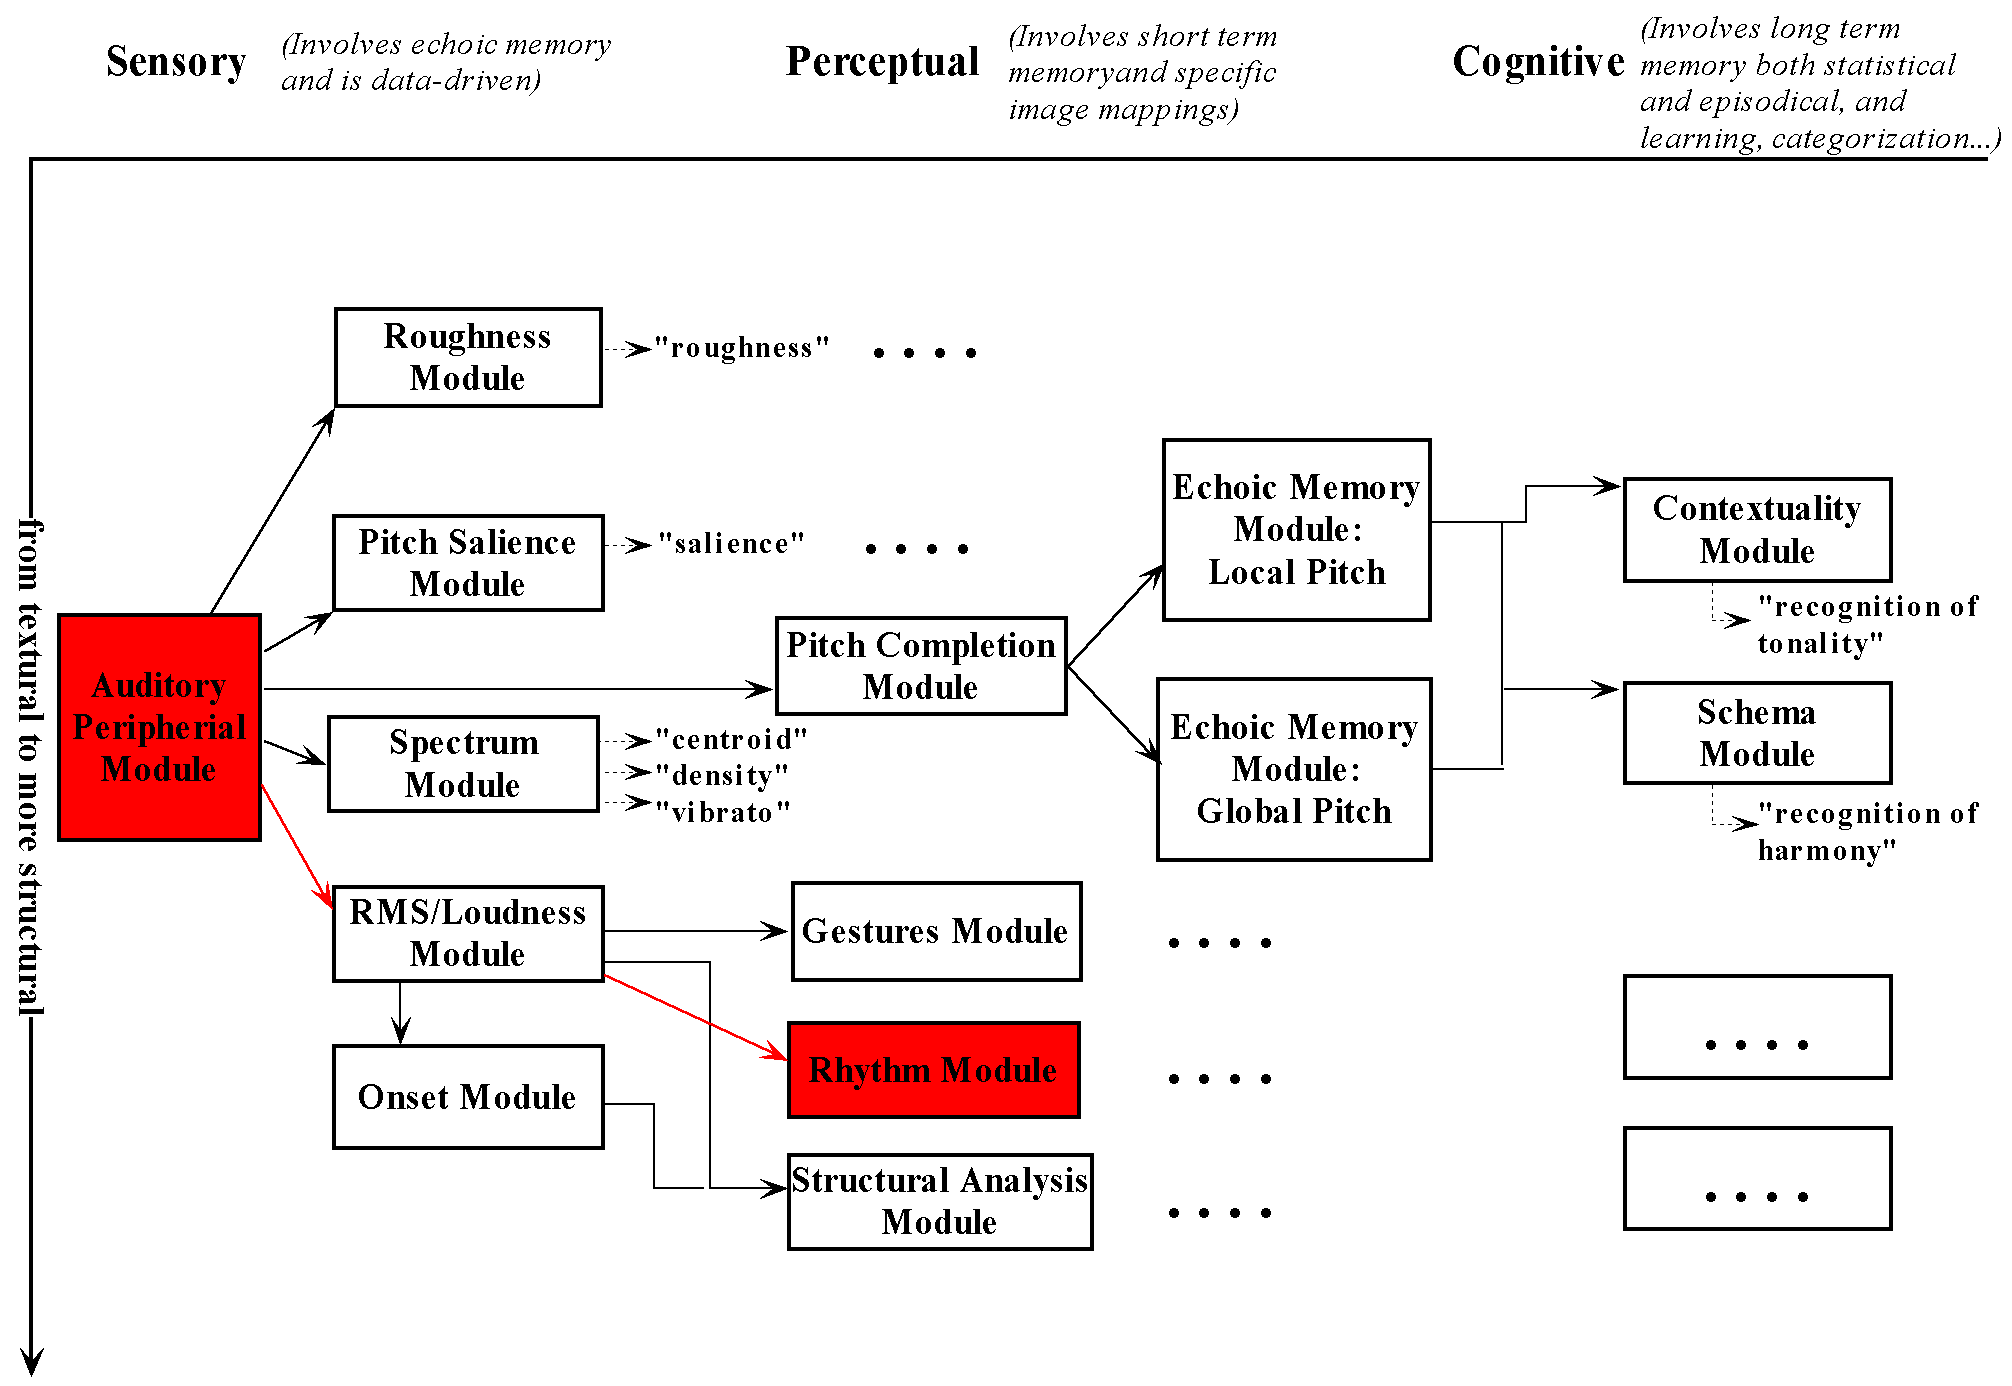
\includegraphics[width=\textwidth]{Graphics/ModulesRhM}
    \caption{Chart of image transformation modules, with RhM highlighted}
    \label{Fig:ModulesRhM}
\end{figure}


\subsection{Functional-logical description}
% --------------------------------------------------------------------------------

The Minimal Energy Change algorithm applied to the recognition of
repetition in rhythm involves:
\begin{eqnarray}
    APM: s(t) \rightarrow e(t,c)\\
    RMS: e(t,c) \rightarrow r(t,c)
\end{eqnarray}
where APM provides the auditory nerve images and where RMS
considers the energy in these images. The application of MEC
involves:
\begin{equation}
    MEC1:  r(t,c) \rightarrow m(\tau,t,c)
\end{equation}
where MEC1 performs a periodicity analysis of these energies and
outputs the estimated periodicity patterns $m(\tau,t,c)$, where
$t$ is time as usual, $\tau$ is the period, and $c$ is the
auditory channel. To obtain the summary MEC-analysis, one has to
sum over all auditory channels, which gives:
\begin{equation}
    MEC2: m(\tau,t) = \sum_{c=1}^{C} m(\tau,t,c)~=~\tilde{m}(t)
\end{equation}
Hence, the MEC-function can be summarized as:
\begin{equation}
    MEC:  \tilde{r}(t) \rightarrow \tilde{m}(t)
\end{equation}
In this notation, one should take into account that the tilde
character, indicating a vector representation, applies to
different dimensions. The components of $\tilde{r}(t)$ are the
channels, while the components of $\tilde{m}(t)$ are the different
periods considered in the analysis. A derived value is the
so-called "best period" $p(t)$, which we obtain by taking the
minimum in each $\tilde{m}(t)$ for fixed $t$, hence:
\begin{equation}
    MEC:  \tilde{r}(t) \rightarrow \tilde{m}(t) \rightarrow p(t)
\end{equation}


\subsection{Signal processing description}
% --------------------------------------------------------------------------------

The MEC-algorithm takes a signal $s(t)$ and its shifted version
$s(t-\tau)$. It then calculates the difference between both
signals, takes the absolute value, and integrates the result:
\begin{equation}\label{MECM1}
    a(\tau,t)~=~
    \int_{0}^{t}~\left|~
    s(t'-\tau)-s(t') ~\right|~
    ~dt'
\end{equation}
where $a(\tau,t)$ at fixed $t$ contains an analysis for all
$\tau$. $\tau$ is typically chosen in the region of interest. For
rhythm detection, this may be from 400 ms to 1 s. The obtained
analysis $a(\tau,t)$ at fixed $t$ is then searched for a minimum:
\begin{equation}\label{MECM2}
    p(t) = ~min_{\tau>0}~a(\tau,t)
\end{equation}
which gives a value $p$ for the best period at each time step $t$.

In practice, we can build in more stability by leaky-integrating
the $a(\tau,t)$ over $t$:
\begin{equation}\label{MECM1B}
    a(\tau,t)~=~
    \int_{0}^{t}~\left|~
    s(t'-\tau)-s(t') ~\right|~
    e^{\beta(t-t')}~dt'
\end{equation}
and apply Expression \ref{MECM2}.

When applied to the signal in different auditory channels, the
calculation will be applied to each channel, thus giving
$a(\tau,t,c)$. To get the best period, one may calculate $p(t)$
using $\sum_{c=1}^{C}a(\tau,t,c)$.


\subsection{Implementation}
% --------------------------------------------------------------------------------

\begin{tabularx}{\linewidth}{llX}
\hyperlink{FuncRef:IPEMMECAnalysis}{IPEMMECAnalysis} & - & Performs a periodicity analysis of a (multi-channel) signal using the MEC model\\
\hyperlink{FuncRef:IPEMMECExtractPatterns}{IPEMMECExtractPatterns} & - & Extracts the best pattern from the original signal using the results of an IPEMMECAnalysis run\\
\hyperlink{FuncRef:IPEMMECReSynthUI}{IPEMMECReSynthUI} & - & User interface callback function for interactively handling the resynthesis of MEC analysis results\\
\hyperlink{FuncRef:IPEMMECSaveResults}{IPEMMECSaveResults} & - & Utility function that saves the results of IPEMMECExtractPatterns, so that resynthesis can still be done at a later date, after reloading this data\\
\hyperlink{FuncRef:IPEMMECSynthesis}{IPEMMECSynthesis} & - & Generates an AM modulated noise signal constructed from a repetition of the pattern found at the specified time moment\\
\end{tabularx}


\subsection{Examples}
% --------------------------------------------------------------------------------

The first steps involve the preparation of the signal in which we
want to look for periodicity. This is done by:\\

\begin{IPEMCodeEnvironment}
[ANI,ANIFreq,ANIFilterFreqs] = IPEMCalcANIFromFile('SchumannKurioseGeschichte.wav');
\newline [RMS,RMSFreq] = IPEMCalcRMS(ANI,ANIFreq,0.050,0.020);
\newline [Periods,Best,AnalysisFreq,Values] = IPEMMECAnalysis(RMS,RMSFreq,0.5,3,[],1.5);
\end{IPEMCodeEnvironment}\\

The MEC algorithm has stored the periods that were analyzed in
\IPEMCodeExtract{Periods}, the indices (into
\IPEMCodeExtract{Periods}) for the best periods found in each
channel in \IPEMCodeExtract{Best}, and all values $m(\tau,t,c)$ in
\IPEMCodeExtract{Values}. The data format of
\IPEMCodeExtract{Values} is described in
\hyperlink{FuncRef:IPEMMECAnalysis}{IPEMMECAnalysis}. Just to give
you an example of how to work with MATLAB, we sum over all
channels $c$ in the following way:\\

\begin{IPEMCodeEnvironment}
SummaryPeriodicity = zeros(size(Values\{1\}));
\newline for channel = 1:40;
\newline SummaryPeriodicity = SummaryPeriodicity + Values\{channel\};
\newline end
\end{IPEMCodeEnvironment}\\

The values in \IPEMCodeExtract{SummaryPeriodicity} contain the
periodicity analysis over all channels which can be visualized
using the MATLAB code:\\

\begin{IPEMCodeEnvironment}
figure;
\newline imagesc((0:size(SummaryPeriodicity,2)-1)/AnalysisFreq,Periods,SummaryPeriodicity);
\newline xlabel('Time (in s)'); ylabel('Period (in s)');
\newline axis xy; colormap(1-gray);
\end{IPEMCodeEnvironment}\\

We plot the best periods of the summary periodicity on top of the
image.\\

\begin{IPEMCodeEnvironment}
[M,I]=min(SummaryPeriodicity); hold on;
\newline plot((0:length(I)-1)/AnalysisFreq,Periods(I));
\end{IPEMCodeEnvironment}\\

The resulting graph should be similar to the one in figure
\ref{Fig:RhMDifferenceValuesSchumannn}.

\begin{figure}[h]
    \centering
    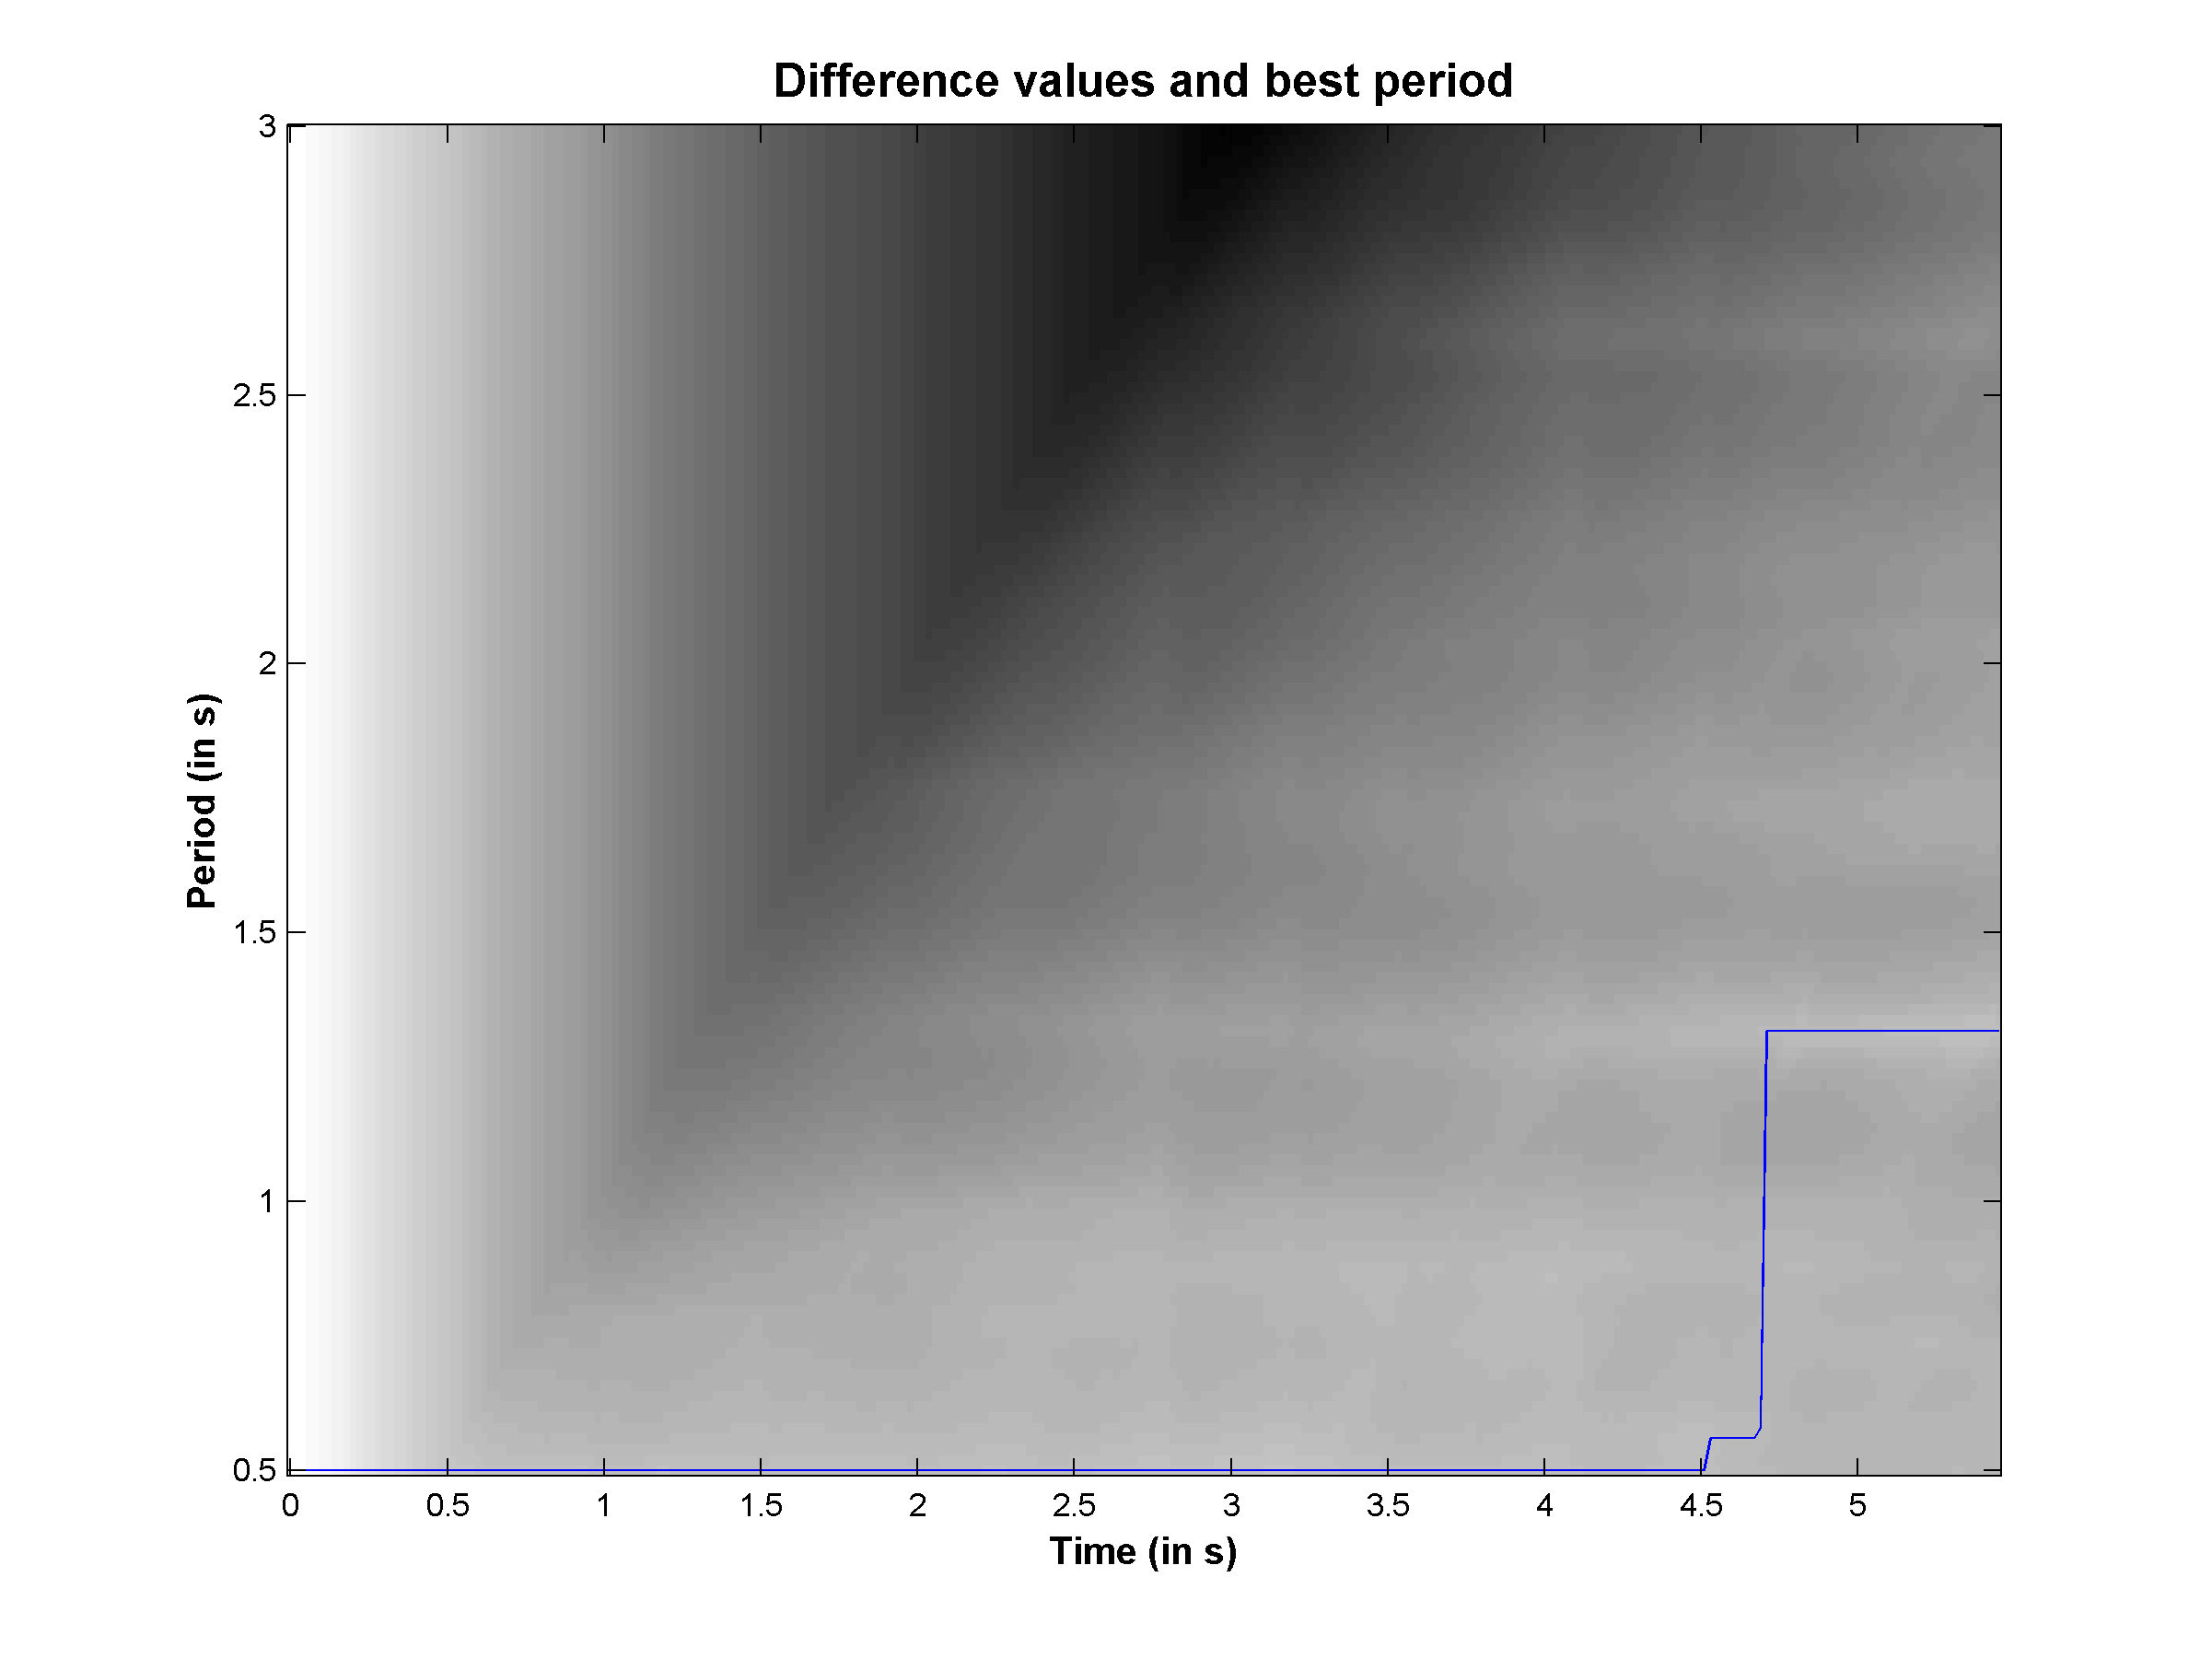
\includegraphics[width=\IPEMDefaultFigureWidth]{Graphics/RhMDifferenceValuesSchumannn}
    \caption{MEC analysis result of a short excerpt of Schumann's Kuriose Geschichte. Shown are the summed difference values (over all channels) and a plot of the best period on top of this.}
    \label{Fig:RhMDifferenceValuesSchumannn}
\end{figure}

% --------------------------------------------------------------------------------

% --------------------------------------------------------------------------------
% --------------------------------------------------------------------------------
\newpage
\section{Echoic Memory Module}
% --------------------------------------------------------------------------------

% Make general target
\hypertarget{Concepts:EchoicMemoryModule}{}

% Make target for following functions:
\hypertarget{Concepts:IPEMLeakyIntegration}{}

\subsection{Introductory description}
% --------------------------------------------------------------------------------

An echo can be defined as a leaky integration with a given half
decay time. At each moment in time, a leaky integrator adds the
incoming signal value to an attenuated version of the previously
calculated value to form the newly calculated value. The half
decay time specifies the time it takes for an impulse signal to
reach half its original value.

The Echoic Memory Module (EMM) takes an image as input and gives
the leaky integrated image as output. The images are integrated so
that at each time step, the new image is calculated by taking a
certain amount of the old image which is then added with the new
incoming image.

The Echoic Memory Module can be applied to pitch completion
images, for example. We then start from our familiar APM, followed
by PCM, and apply EMM. The echo which we specify defines the
amount of context which we take into account. With very little (or
almost no) context we speak about \emph{local pitch images}. When
context is taken into account we use a longer half decay time and
call the images \emph{global pitch images}. EMM has been used in
\citeA{article:MusicPerception:Leman:2000} to construct the
pitch images of an echoic memory. In our global chart of image
transformation modules EMM is localized in the middle part
(perception section) of figure \ref{Fig:ModulesEMM}. The
application is described in detail in the chapter on
\hyperlink{Concepts:IPEMGenerateProbes}{{tonality induction
experiments}}.
\begin{figure}[h]
    \centering
    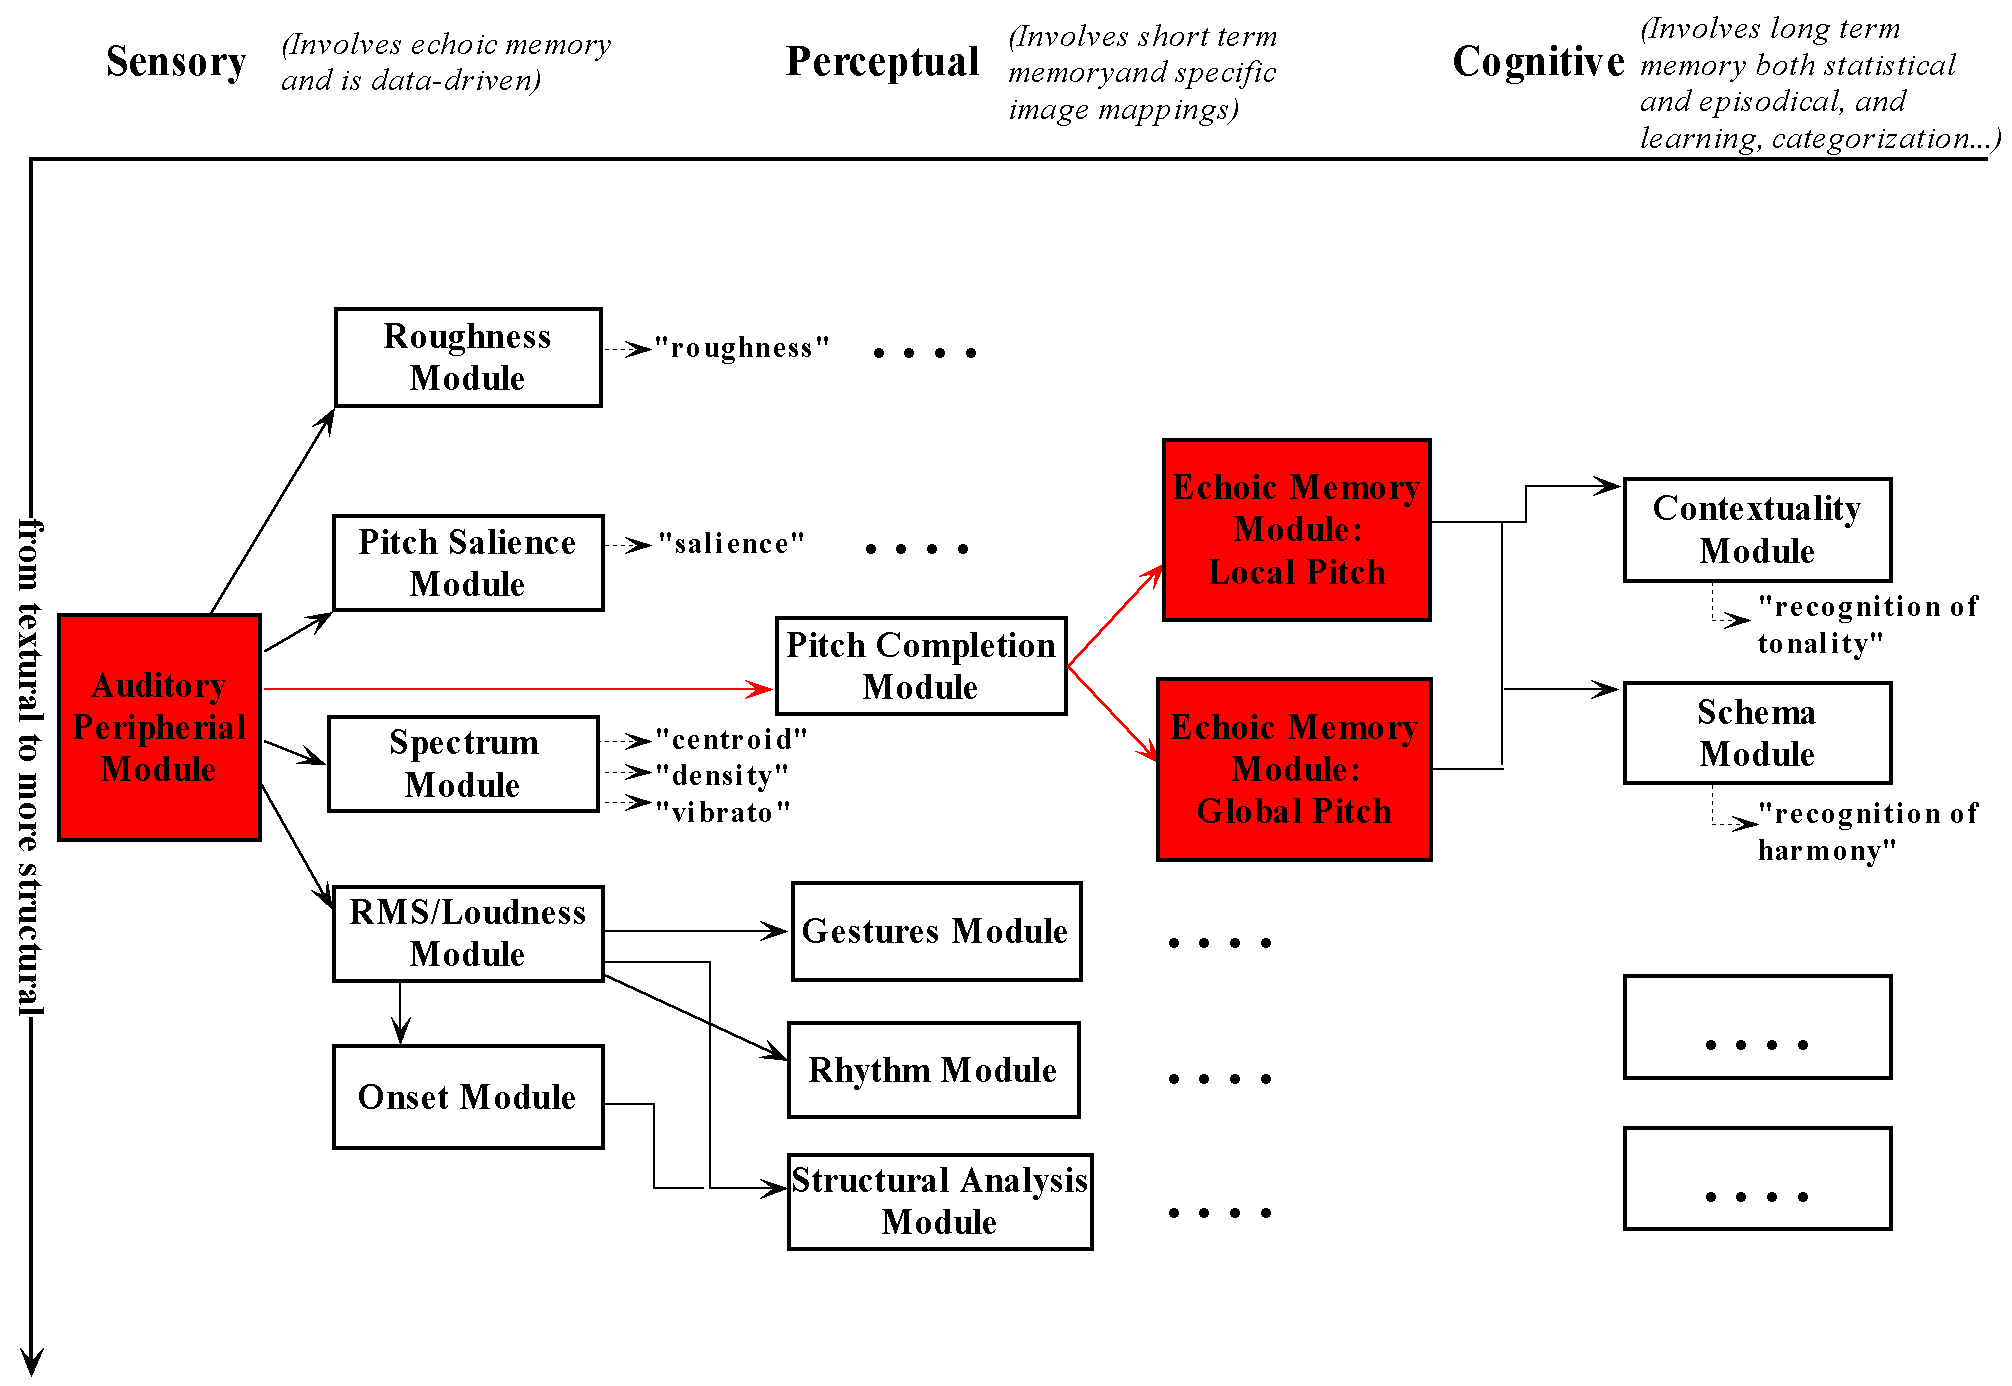
\includegraphics[width=\textwidth]{Graphics/ModulesEMM}
    \caption{Chart of image transformation modules, with EMM highlighted}
    \label{Fig:ModulesEMM}
\end{figure}
Figure \ref {Fig:EMMModule} shows the modules involved in the
image transformation process.
\begin{figure}[h]
    \centering
    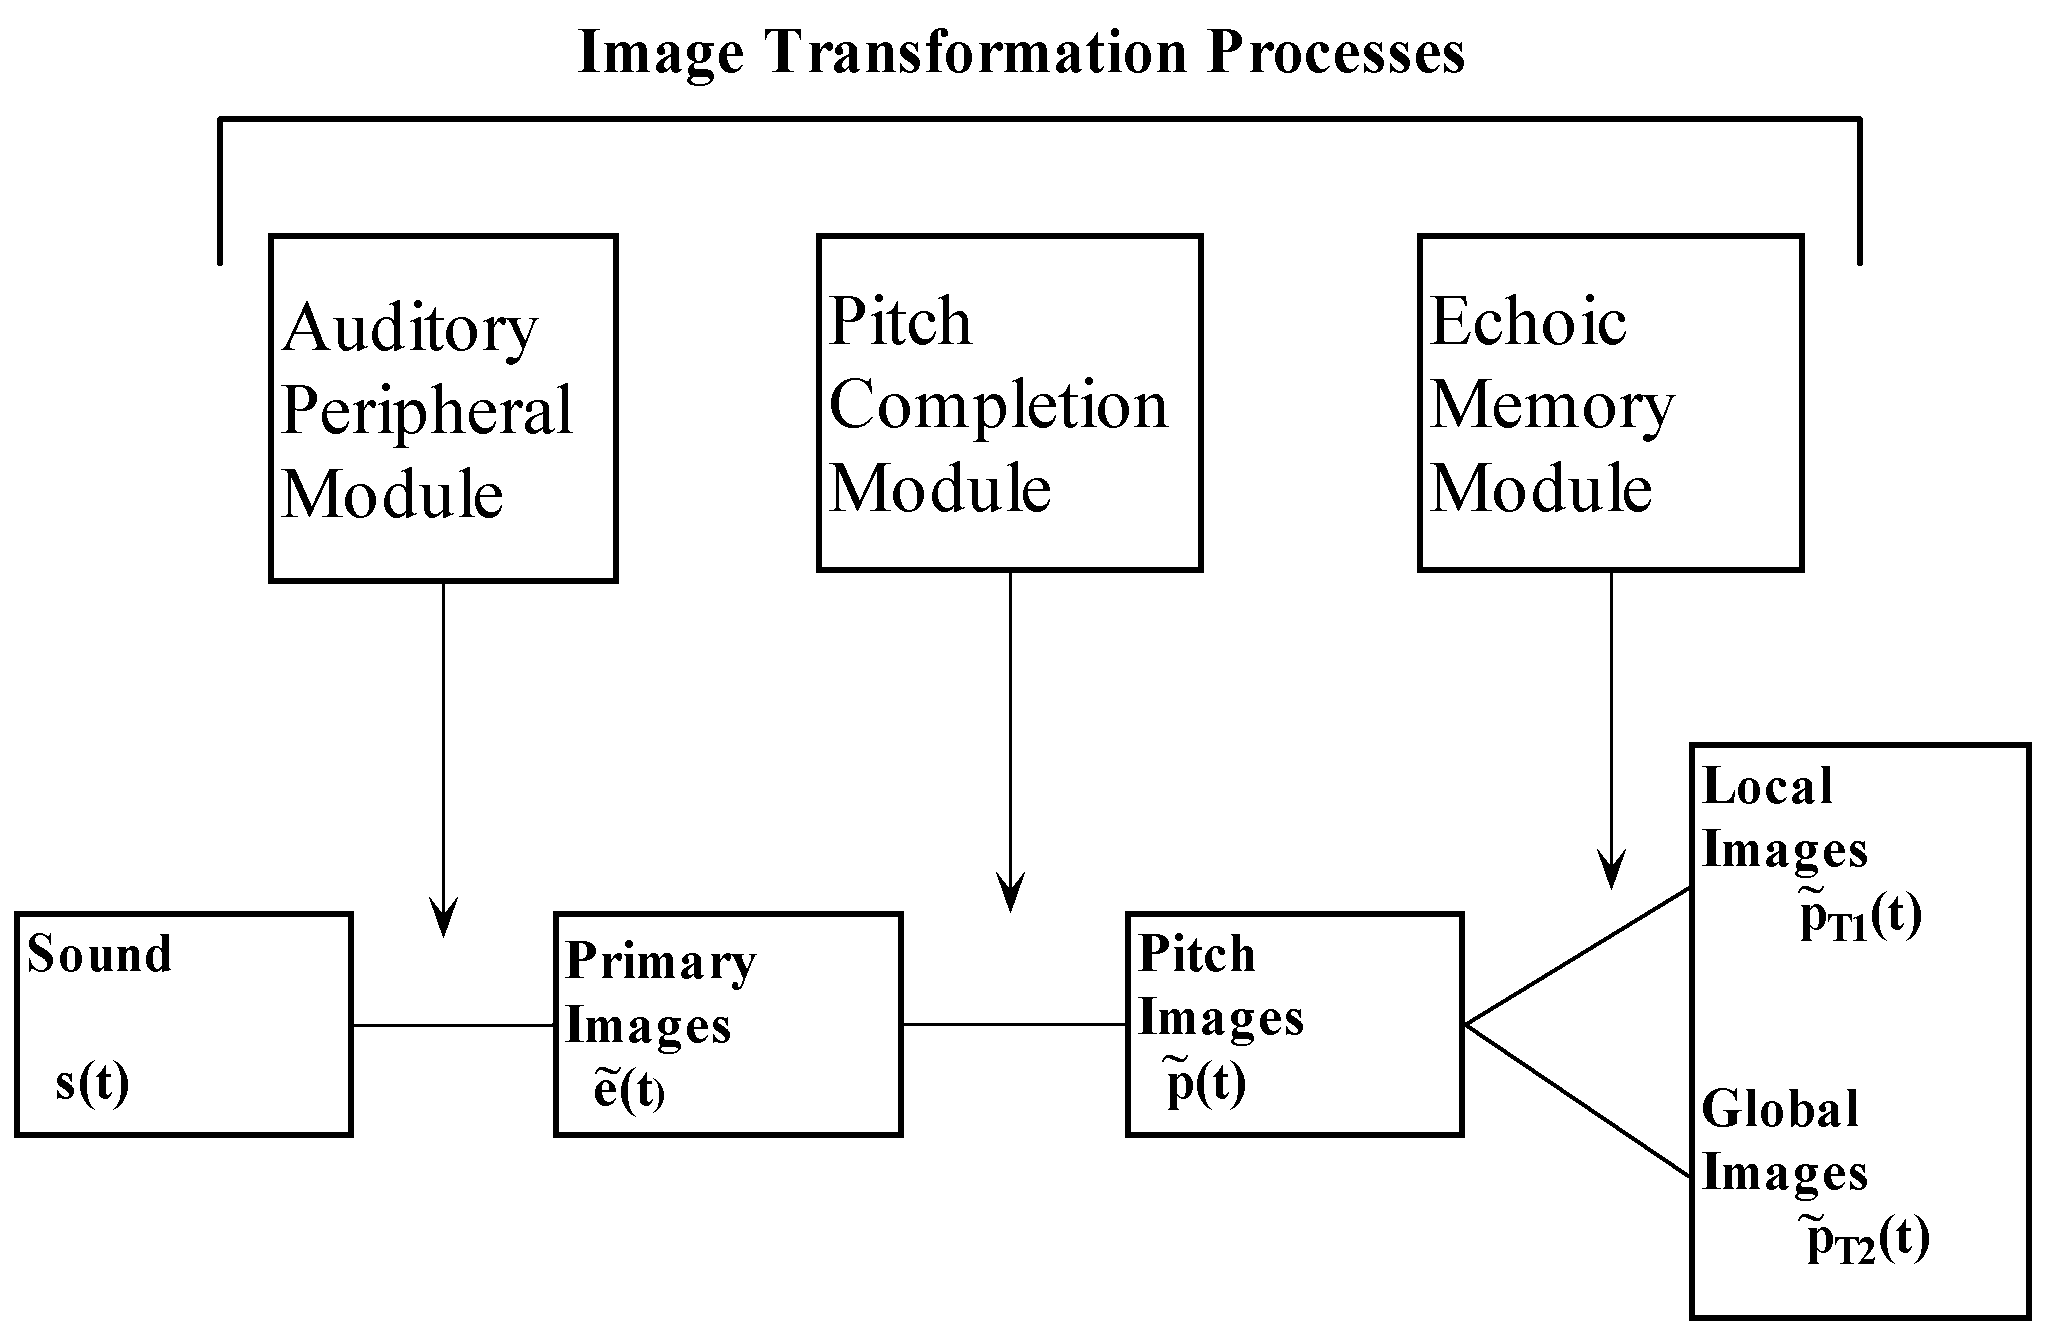
\includegraphics[width=\IPEMDefaultFigureWidth]{Graphics/EMMModule}
    \caption{Image Transformation Process: Echoic Memory Module}
    \label{Fig:EMMModule}
\end{figure}

\subsection{Functional-logical description}
% --------------------------------------------------------------------------------

A symbolic representation of the Echoic Memory Module may be written as:
\begin{equation}
EMM: \tilde{p}(t) \rightarrow \tilde{p}_T(t)
\end{equation}
where $T$ denotes the {\sl echo} in seconds, $\tilde{p}(t)$
denotes a pitch completion image and $ \tilde{p}_T(t)$ an echoed
image.


\subsection{Signal processing description}
% --------------------------------------------------------------------------------

$\tilde{p}_T(0) = \tilde{p}(0)$

$\tilde{p}_T(t) = \tilde{p}(t) ~+~
\tilde{p}_T(t-1)*2^{\frac{-1}{T}}$ \quad , $t \neq 0$


\subsection{Implementation}
% --------------------------------------------------------------------------------

\begin{tabularx}{\linewidth}{llX}
\hyperlink{FuncRef:IPEMLeakyIntegration}{IPEMLeakyIntegration} & - & Calculates leaky integration with specified half decay time\\
\end{tabularx}


\subsection{Examples}
% --------------------------------------------------------------------------------

The Echoic Memory Module can be applied to a pitch completion
image to obtain a local and a global pitch image. A local pitch
image can be defined as $\tilde{p}_{T=0.1}(t)$, with an echo of
0.1 s, while a global pitch image can be defined as
$\tilde{p}_{T=1.5}(t)$, with the echo of 1.5 s. Local images are
built up by echoes which, by definition, are smaller than echoes
for the global images. Use the following MATLAB functions to
create those pitch images:\\

\begin{IPEMCodeEnvironment}
[ANI,ANIFreq,ANIFilterFreqs] = IPEMCalcANIFromFile('SchumannKurioseGeschichte.wav');
\newline [PP,PPFreq,PPPeriods,PPFANI] = IPEMPeriodicityPitch(ANI,ANIFreq);
\newline LocalIntegration = IPEMLeakyIntegration(PP,PPFreq,0.1,0.1,1);
\newline GlobalIntegration = IPEMLeakyIntegration(PP,PPFreq,1.5,1.5,1);
\end{IPEMCodeEnvironment}\\

Figure \ref{Fig:EMMPitchImages} shows the pitch images for the
\IPEMSound{Sounds/SchumannKurioseGeschichte.wav}{excerpt of
Schumann's Kuriose Geschichte}.

\begin{figure}[h]
    \centering
    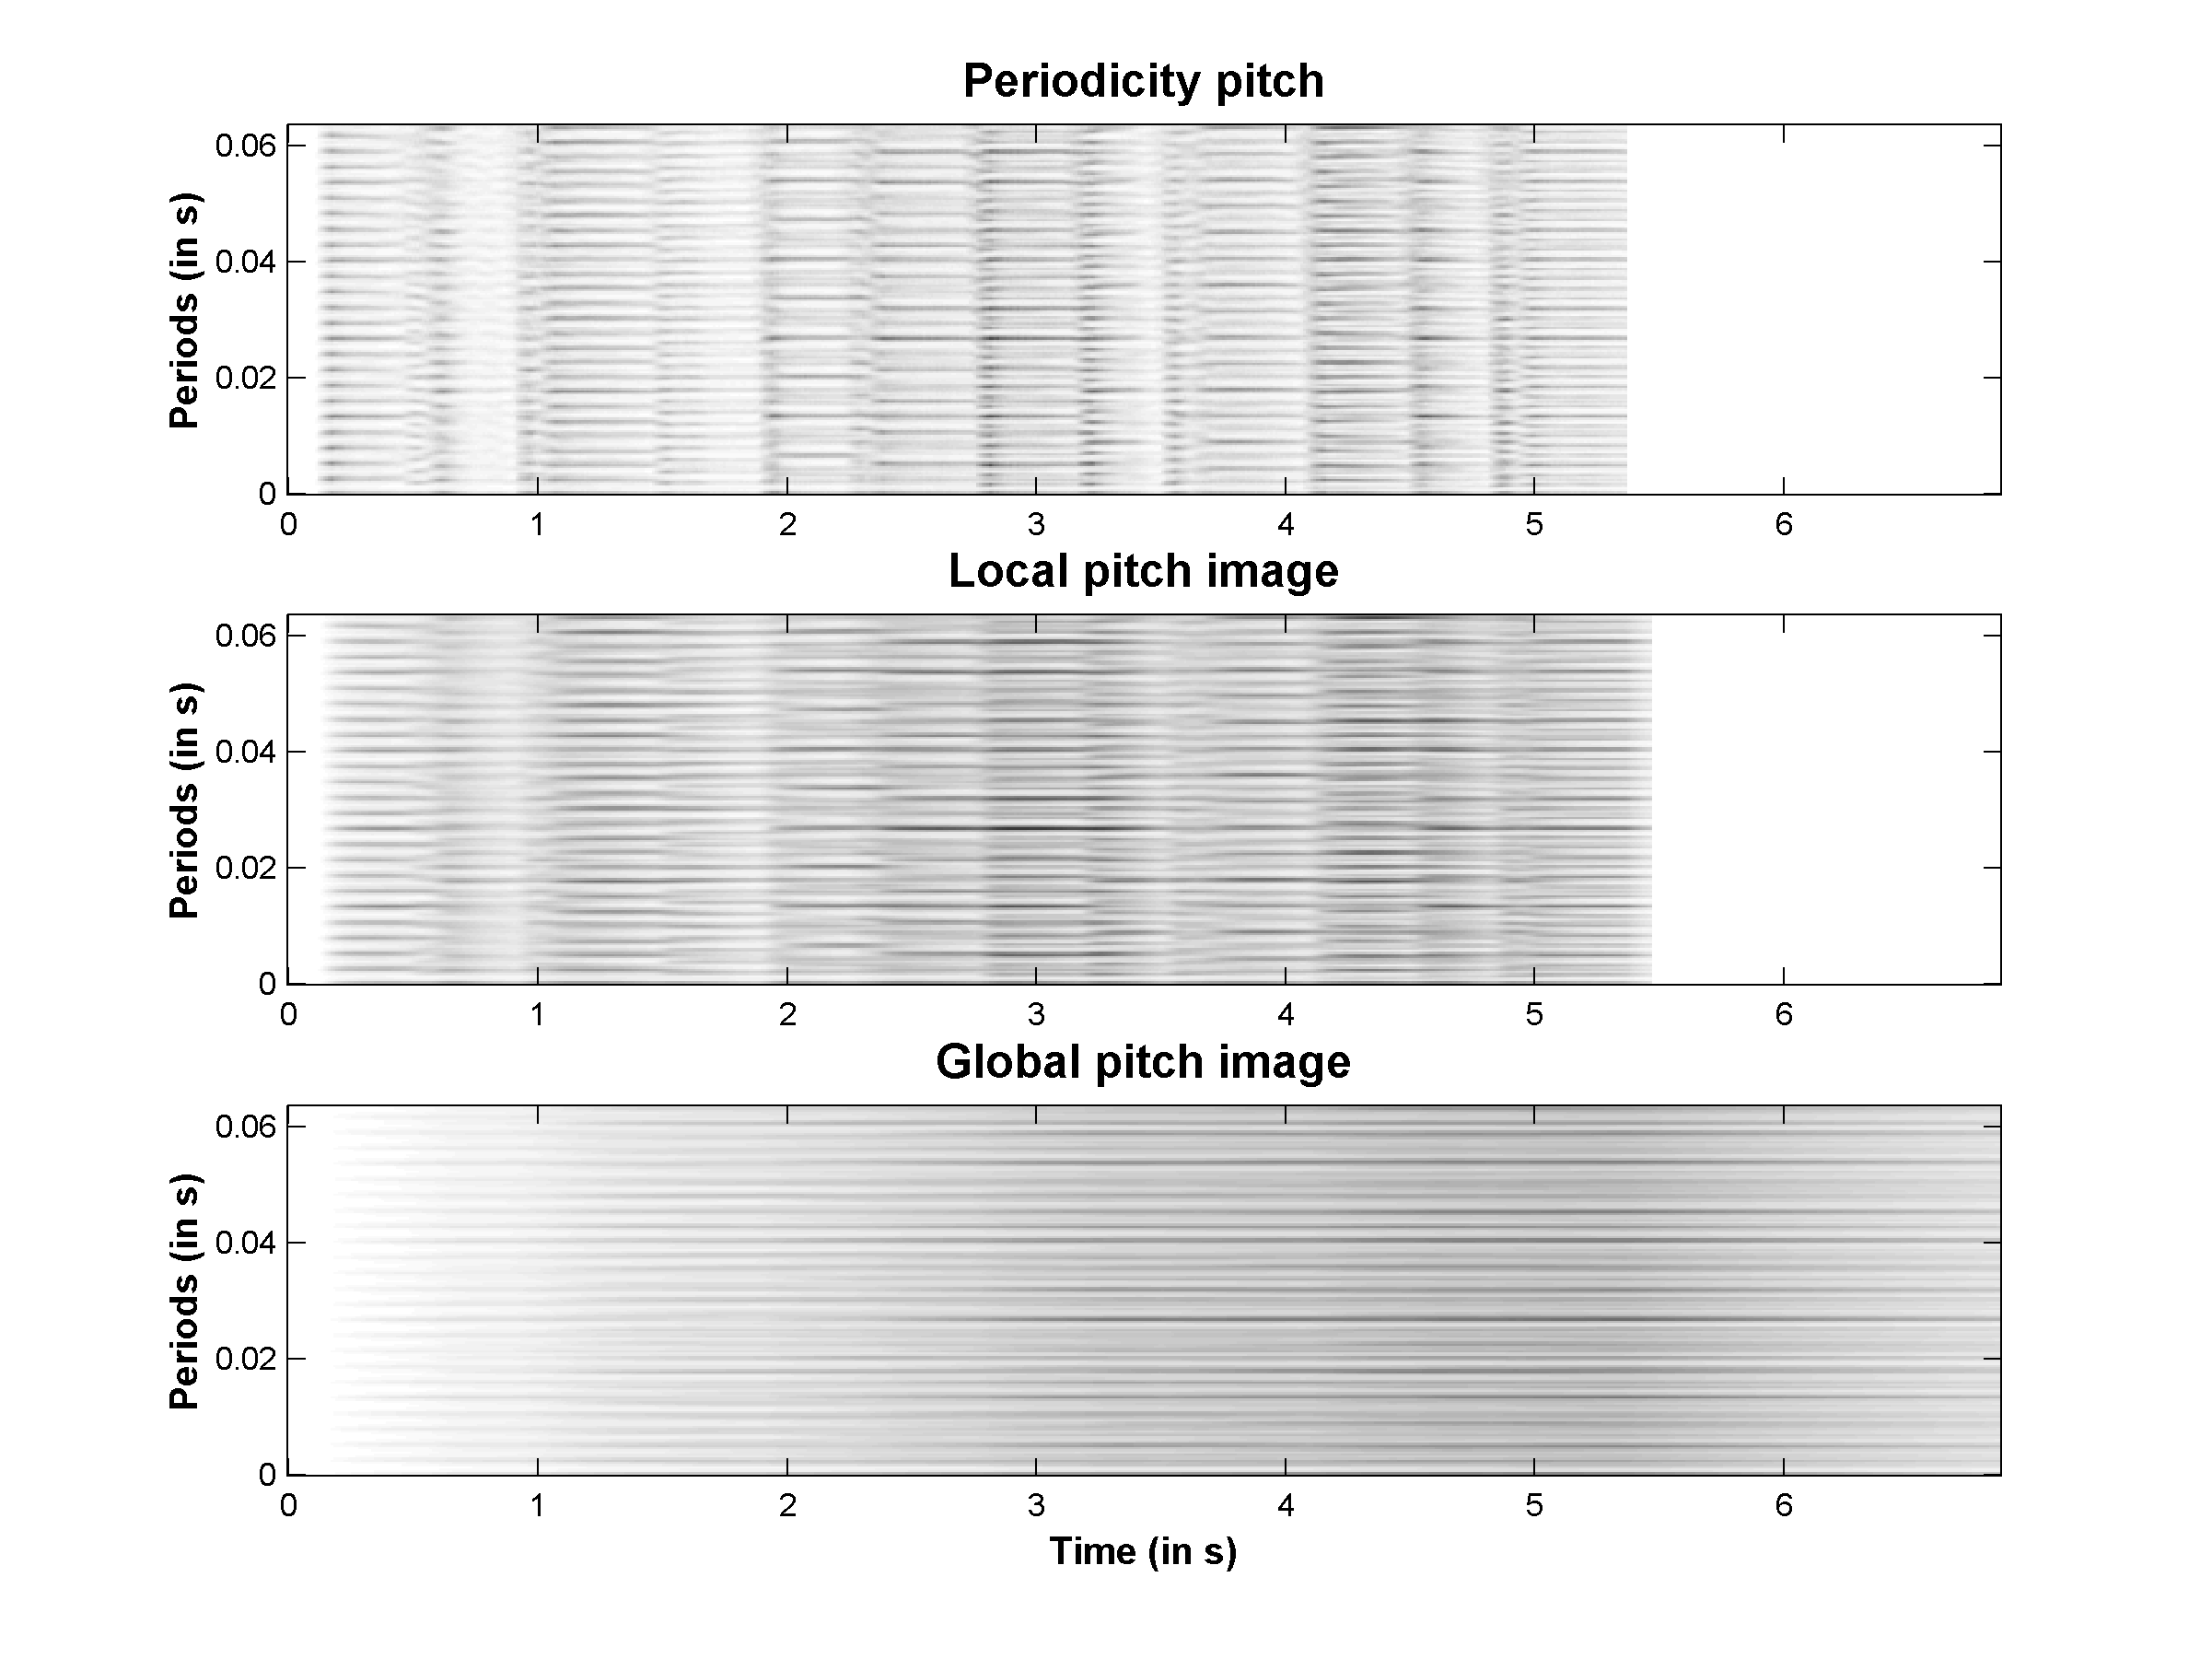
\includegraphics[width=\IPEMDefaultFigureWidth]{Graphics/EMMPitchImages}
    \caption{Top: periodicity pitch for the excerpt of Schumann's Kuriose Geschichte
    Middle: local pitch image of Schumann's Kuriose Geschichte (echo of 0.1 s).
    Bottom: global pitch image (echo of 1.5 s)}
    \label{Fig:EMMPitchImages}
\end{figure}

% --------------------------------------------------------------------------------

% --------------------------------------------------------------------------------
% --------------------------------------------------------------------------------
\newpage
\section{Contextuality Module}
% --------------------------------------------------------------------------------

% Make general target
\hypertarget{Concepts:ContextualityModule}{}

% Make target for following functions:
\hypertarget{Concepts:IPEMContextualityIndex}{}

\subsection{Introductory description}
% --------------------------------------------------------------------------------

Contextuality measures the pitch commonality between two running
pitch images of the same sound, each having a possible different
echo. In \citeA{article:MusicPerception:Leman:2000}, contextuality
is used to measure the pitch commonality of local (=short echo)
images versus global (=long echo) images. Two types of measurement
are taken into account:
\begin{itemize}
\item
    The first method is based on an \emph{inspection} of the pitch sequence by
    means of a fixed image (or \emph{probe}).
\item
    The second method is based on a \emph{comparison} of the pitch images (each
    having a possible different echo) at running time. This amounts to the
    calculation of the differences, due to the echo, between both running images.
\end{itemize}
Inspection and comparison of echoic pitch images are useful
methods for studying tonal tensions in terms of figure/ground
relationships.\\ In our global chart of image transformation
modules CM is localized in the cognitive section of figure
\ref{Fig:ModulesCM}.

\begin{figure}[h]
    \centering
    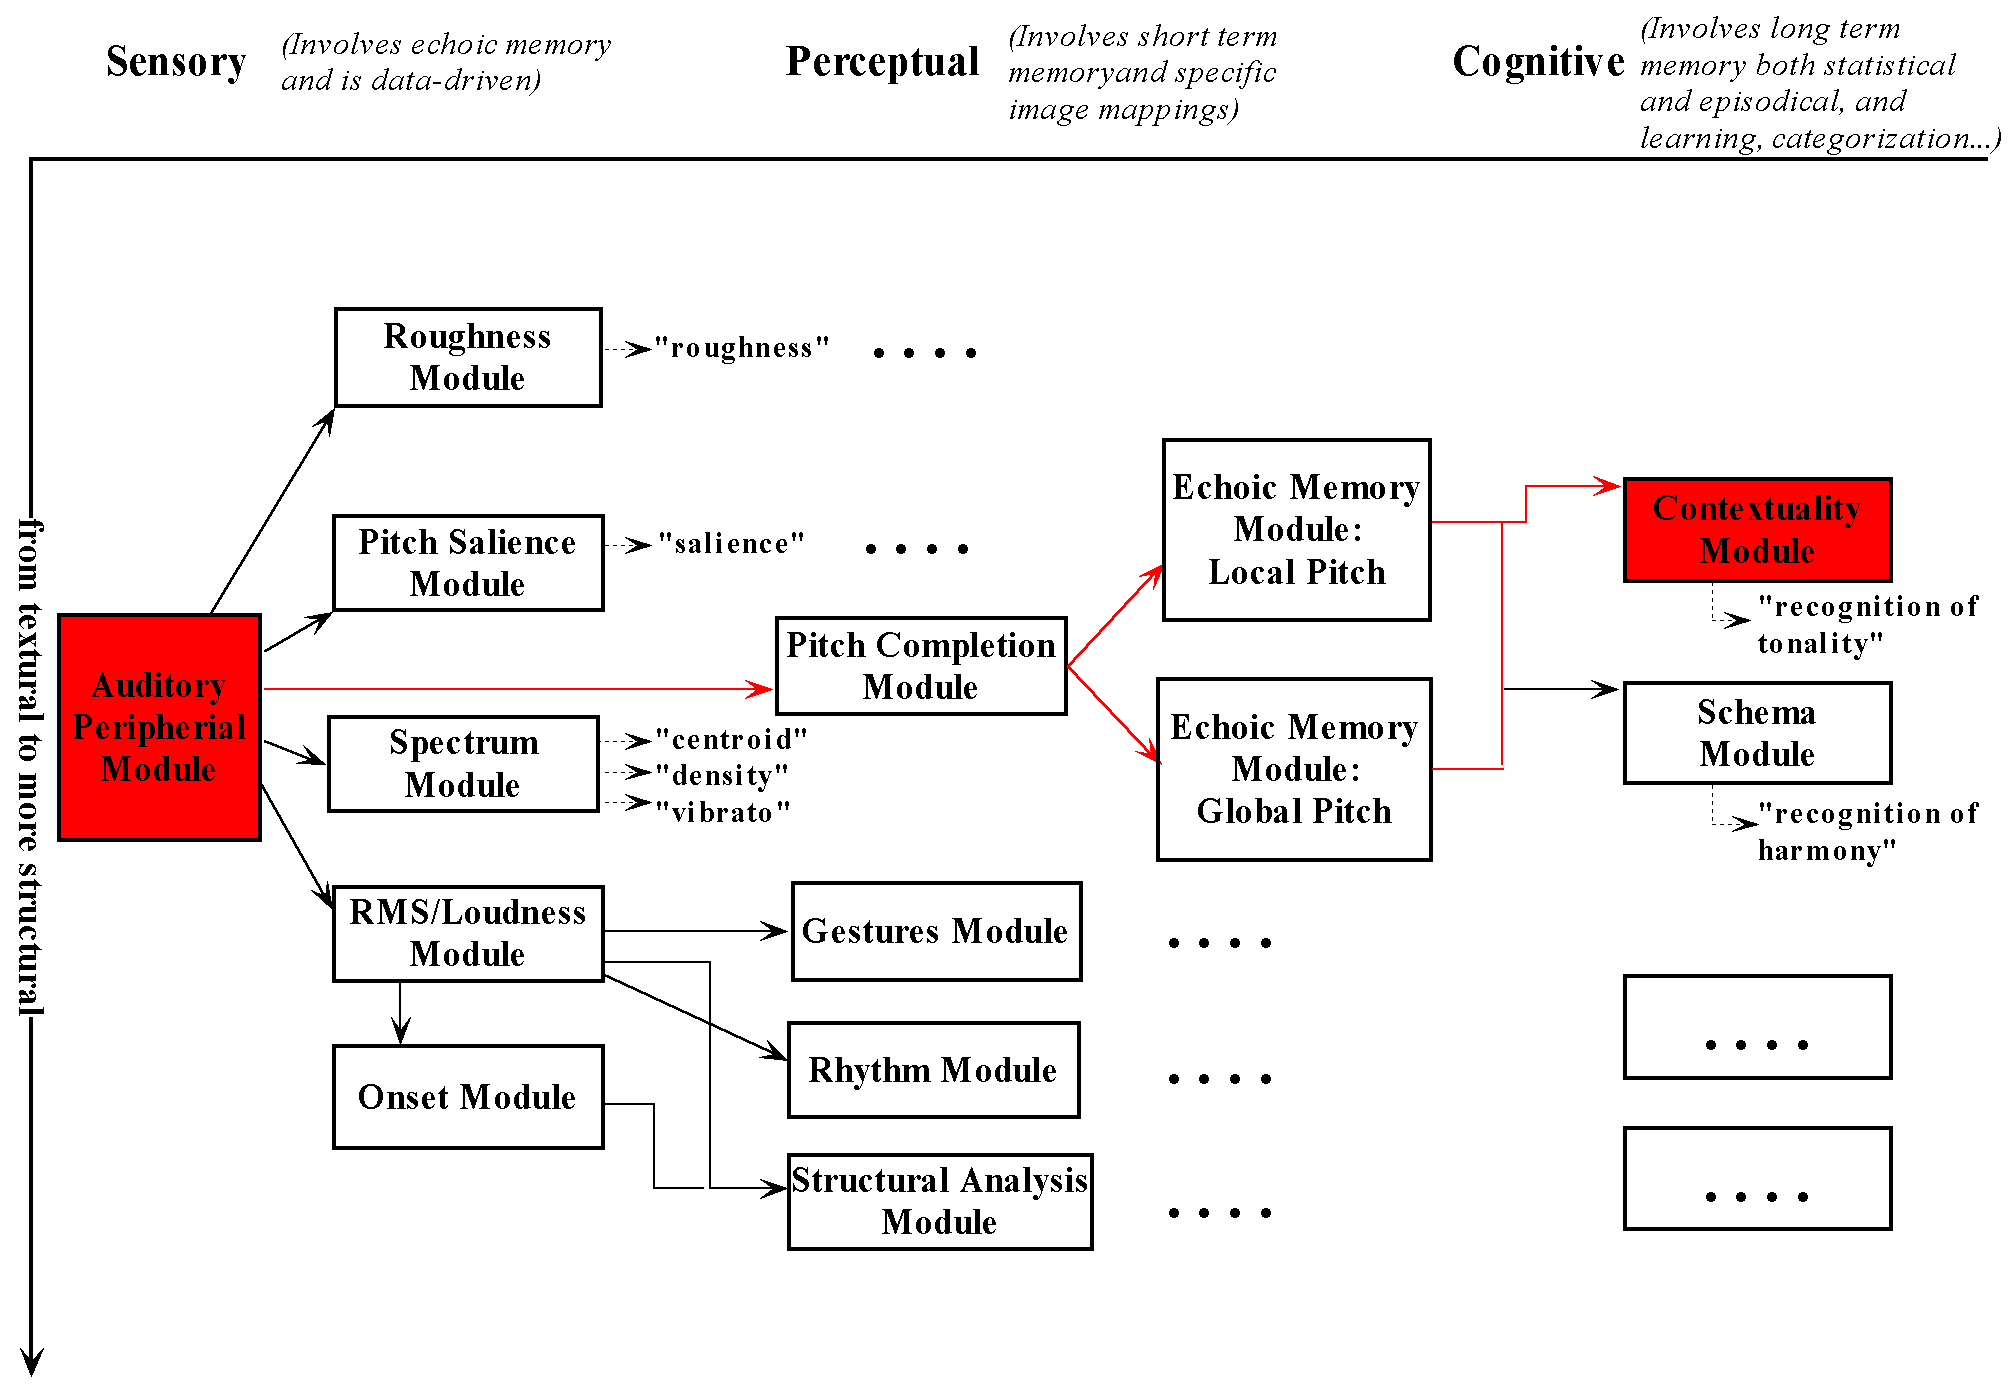
\includegraphics[width=\textwidth]{Graphics/ModulesCM}
    \caption{Chart of image transformation modules, with CM highlighted}
    \label{Fig:ModulesCM}
\end{figure}

Figure \ref{Fig:CMModule} shows the modules involved in the image
transformation and inference process.
\begin{figure}[h]
    \centering
    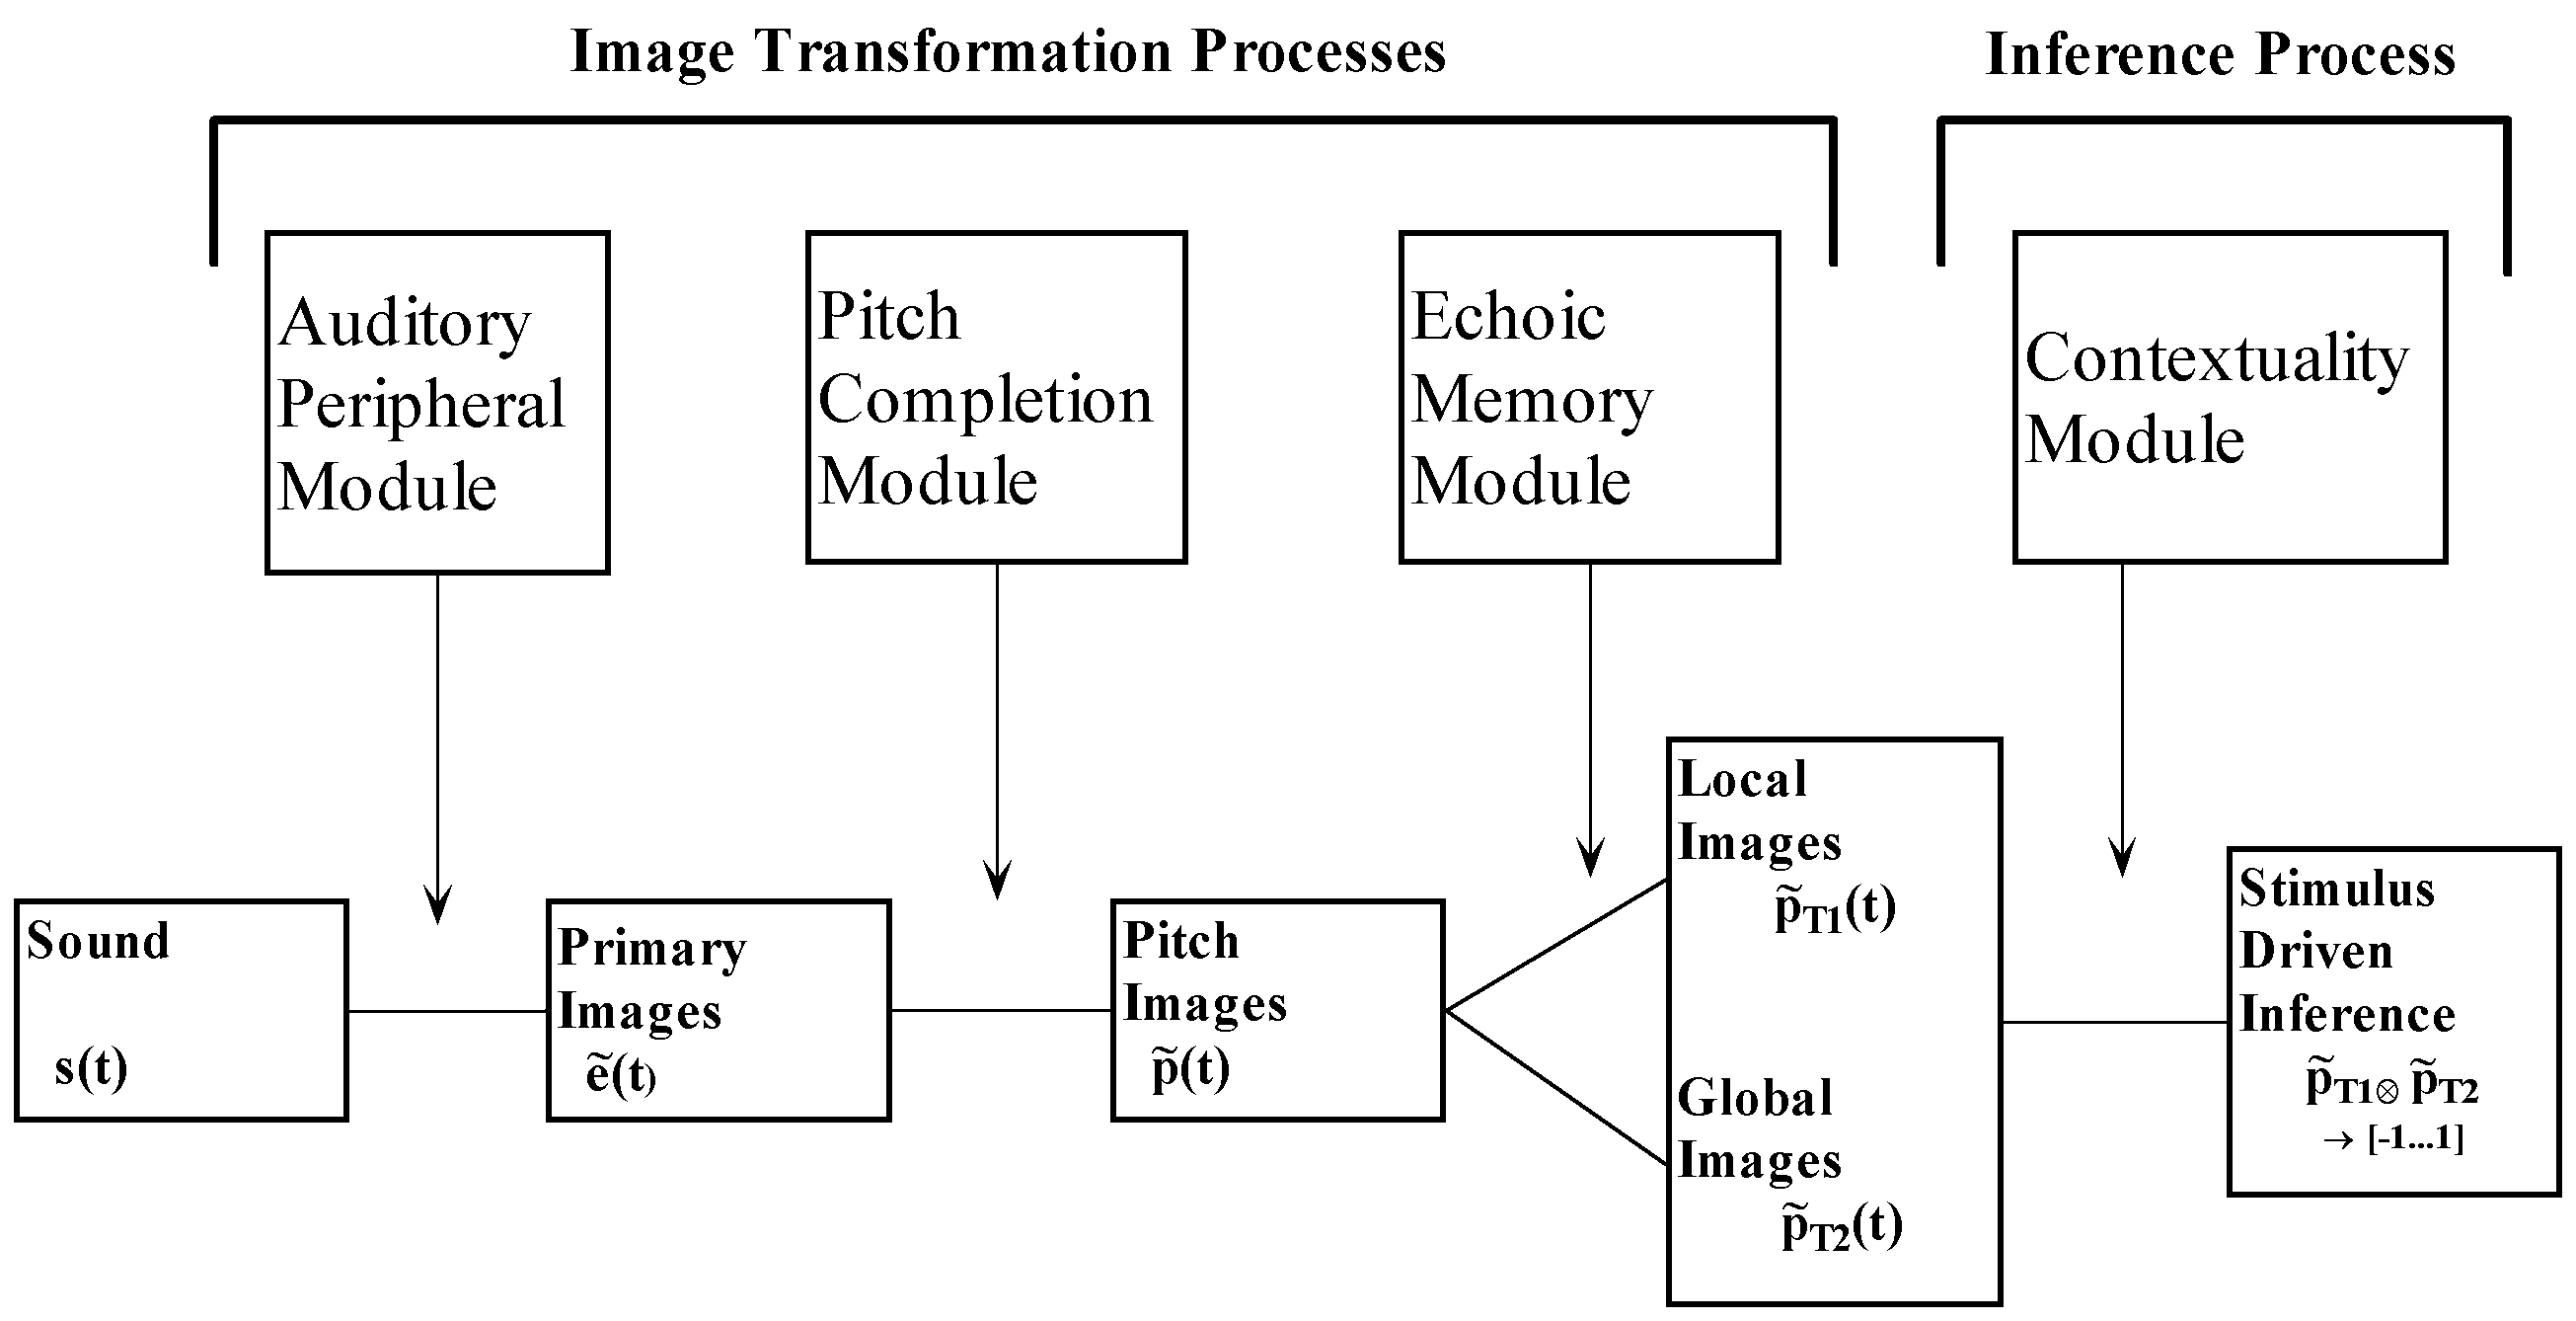
\includegraphics[width=\IPEMDefaultFigureWidth]{Graphics/CMModule}
    \caption{Image Transformation and Inference Process: Contextuality Module}
    \label{Fig:CMModule}
\end{figure}


\subsection{Functional-logical description}
% --------------------------------------------------------------------------------

Contextulatiy realizes a mapping of two images onto a scale:
\begin{equation}
Contextuality: \tilde{p}_{T1} \bigotimes \tilde{p}_{T2} \rightarrow [-1 ... 1]
\end{equation}
where $\tilde{p}$ is a pitch image,
$T1$ and $T2$ are standing for the respective echoes (with T1 $\leq$ T2),
and $\bigotimes$ represents the calculation of a correlation coefficient.
The two methods then correspond to the following mappings:
\begin{itemize}
\item{Inspection:}
    \begin{displaymath}
    Contextuality_{I}: \tilde{p}_{T1}(\tau) \bigotimes \tilde{p}_{T2}(t) \rightarrow [-1 ...
    1]
    \end{displaymath}
    where $\tau$ represents a fixed time instance, typically situated at the end of the
    sound sequence, and $t$ represents the running time.
\item{Comparison:}
    \begin{displaymath}
    Contextulatiy_{II}: \tilde{p}_{T1}(t) \bigotimes \tilde{p}_{T2}(t) \rightarrow [-1 ...
    1]
    \end{displaymath}
    where $t$ represents the running time for both images.
\end{itemize}


\subsection{Signal processing description}
% --------------------------------------------------------------------------------

The Contextuality Module involves several modules.
\begin{itemize}
\item
    The auditory nerve image is calculated using the
    \hyperlink{Concepts:AuditoryPeripheralModule}{Auditory Peripheral
    Module}
\item
    The \hyperlink{Concepts:PitchCompletionModule}{Pitch Completion
    Module} transforms the auditory nerve image into pitch images
\item
    Through the \hyperlink{Concepts:EchoicMemoryModule}{Echoic Memory
    Module} the pitch images undergo the effect of an echo and are
    processed into local and global images
\item
    The Contextuality Module considers two types of contextuality
\end{itemize}


\subsection{Implementation}
% --------------------------------------------------------------------------------

\begin{tabularx}{\linewidth}{llX}
\hyperlink{FuncRef:IPEMContextualityIndex}{IPEMContextualityIndex}
& - & Calculates the contextuality index. Two methods are used:
the method of comparison compares running chords with running tone
center images, while the method of inspection compares a fixed
chord with running chords and running tone center images.
\end{tabularx}


\subsection{Examples}
% --------------------------------------------------------------------------------

Contextuality has been used to simulate the probe-tone experiments
of Krumhansl and Kessler
\cite{article:MusicPerception:Leman:2000,KrumhanslKessler:82}.
%See also \hyperlink{Chapter:ConceptsApplications}{Applications} for more elaborate examples.\\

In what follows, contextuality is applied to the
\IPEMSound{Sounds/SchumannKurioseGeschichte.wav}{short excerpt of
Schumann's Kuriose Geschichte} followed by a 0.1 s period of
silence and an f$\sharp$ Shepard tone. Use the following MATLAB
code to read in the sound file, generate the silence and generate
the Shepard tone f$\sharp$:\\

\begin{IPEMCodeEnvironment}
[s1,fs] = IPEMReadSoundFile('SchumannKurioseGeschichte.wav');
\newline s2 = zeros(1,round(0.1*fs));
\newline NoteFreq = IPEMCalcNoteFrequency('F\#4');
\newline s3 = IPEMShepardTone(NoteFreq,0.5,fs,1,-20);
\end{IPEMCodeEnvironment}\\

Concatenate the 3 sound signals, calculate the auditory nerve
image and from there the periodicity pitch (see also
\hyperlink{Concepts:EchoicMemoryModule}{Echoic Memory Module})
using the following Matlab code:\\

\begin{IPEMCodeEnvironment}
s = [s1 s2 s3];
\newline [ANI,ANIFreq,ANIFilterFreqs] = IPEMCalcANI(s,fs);
\newline [PP,PPFreq,PPPeriods,PPFANI] = IPEMPeriodicityPitch(ANI,ANIFreq,[],[],[],1);
\end{IPEMCodeEnvironment}\\

Then finally, the function
\hyperlink{FuncRef:IPEMContextualityIndex}{IPEMContextualityIndex}
 is applied for the context analysis.\\

\begin{IPEMCodeEnvironment}
[Chords,ToneCenters,LocalInspection,GlobalInspection,LocalGlobalComparison] = ...
\newline IPEMContextualityIndex(PP,PPFreq,PPPeriods,[],0.1,1.5,[],1);
\end{IPEMCodeEnvironment}\\

In this example, \IPEMCodeExtract{PP} contains the periodicity
pitch image of the concatenated sounds, \IPEMCodeExtract{PPFreq}
contains the sampling rate, \IPEMCodeExtract{PPPeriods} contains
the analyzed periods, and the fourth argument specifies the
location of the fixed image. Here, it is left blank, which
defaults to the end of the signal. The local and global echoes are
set to 0.1 s and 1.5 s, respectively, and the plot flag is set to
1.\\

Figure \ref{Fig:ContextualityPitchImages} shows the periodicity
pitch image of the Schumann excerpt followed by the Shepard tone,
the local pitch image, and the global pitch image.\\
The method based on inspection has been applied to the local and
the global pitch images.\\

\IPEMCodeExtract{LocalInspection}
(fig. \ref{Fig:ContextualityLocalInspection}) contains the results
of inspecting the local images with the fixed (local) image. The
graph shows the similarity of the Shepard probe tone of
f$\sharp$ within the Schumann excerpt at a local level.\\

\IPEMCodeExtract{GlobalInspection}
(fig. \ref{Fig:ContextualityGlobalInspection}) contains the
results of inspecting the global images with the fixed (local)
image. The graph shows the similarity of the Shepard probe tone of
f$\sharp$ within the Schumann excerpt at a more global pitch
level.\\

\IPEMCodeExtract{LocalGlobalComparision}
(fig. \ref{Fig:ContextualityLocalGlobalComparison}) contains the
results of comparing the local images with the global images over
the whole piece. It shows the degree in which the local pitch
images (= the level of individual tones and chords) fit with the
global pitch images (= the level of the tone context). At points
where the local image deviates from the global image, such as in a
tonal movement, there will be a low correlation. Inversely, at
points where the local image confirms the global image, there will
be a high correlation.\\

\begin{figure}[h]
    \centering
    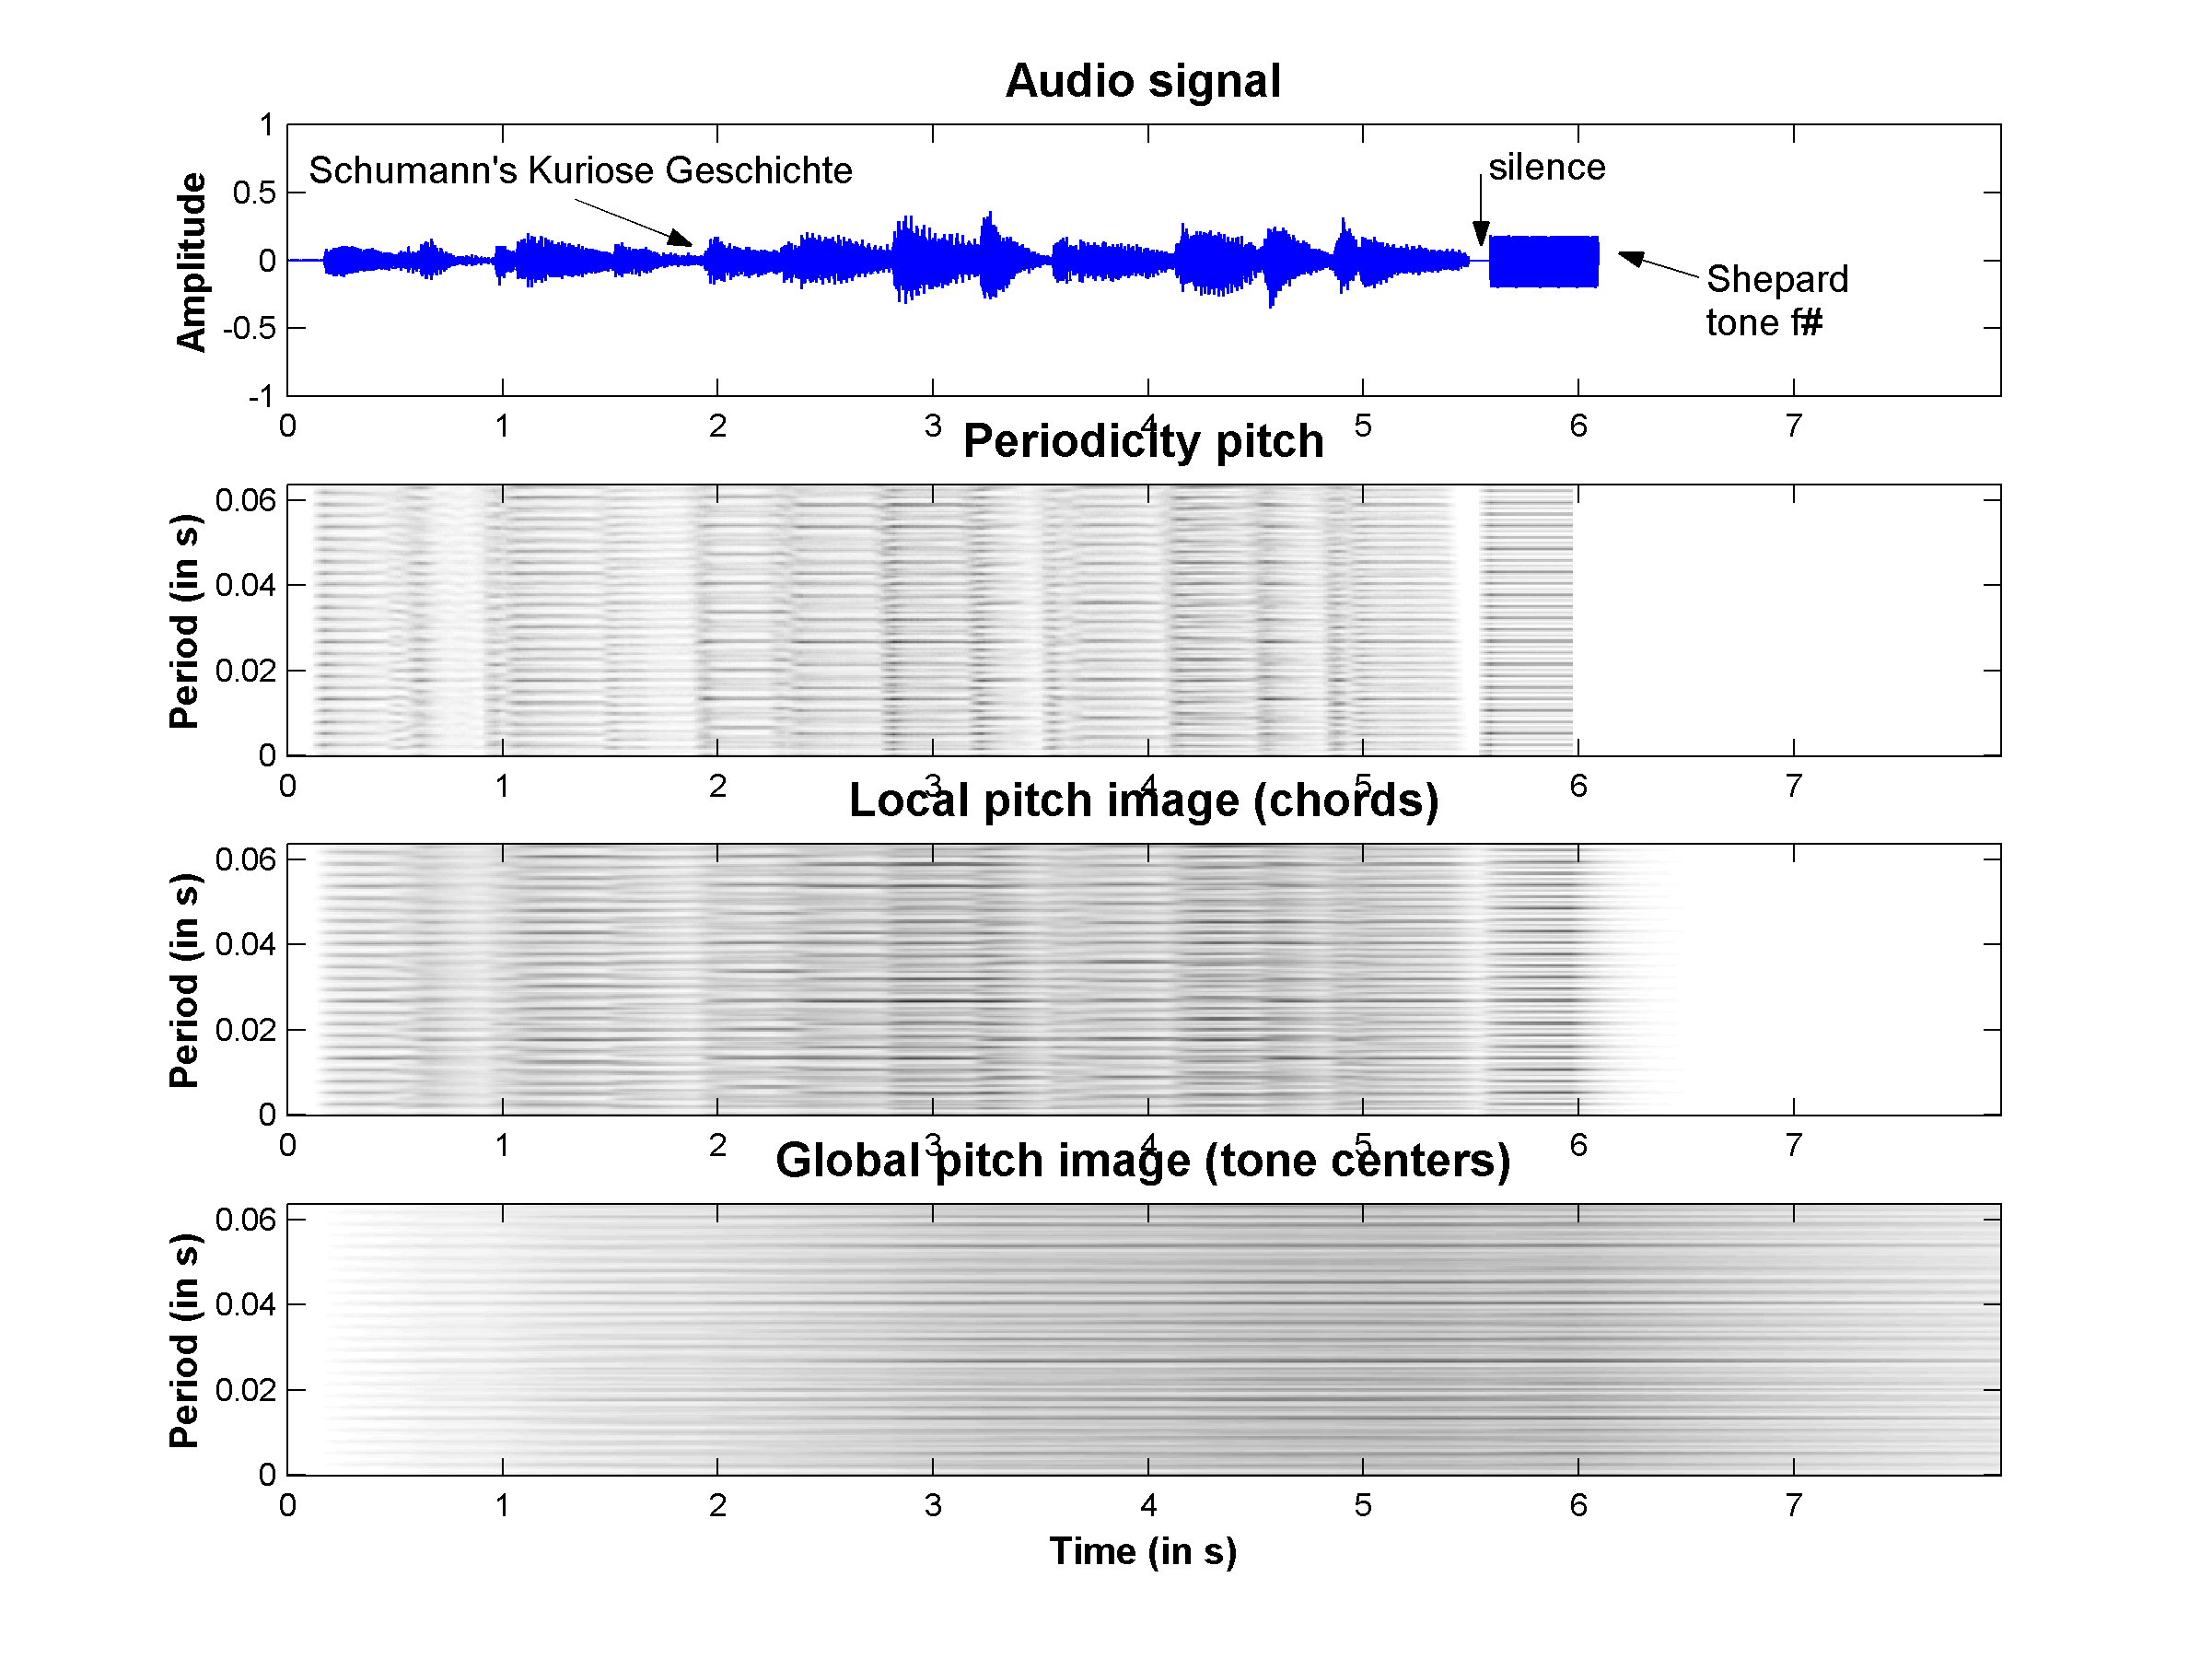
\includegraphics[width=\IPEMDefaultFigureWidth]{Graphics/ContextualityPitchImages}
    \caption{Pitch images for the excerpt of Schumann's Kuriose
    Geschichte followed by a small period of silence and a Shepard
    probe-tone of f$\sharp$. From top to bottom: the analyzed
    audio signal, the periodicity pitch image, the local pitch image and
    the global pitch image.} \label{Fig:ContextualityPitchImages}
\end{figure}

\begin{figure}[h]
    \centering
    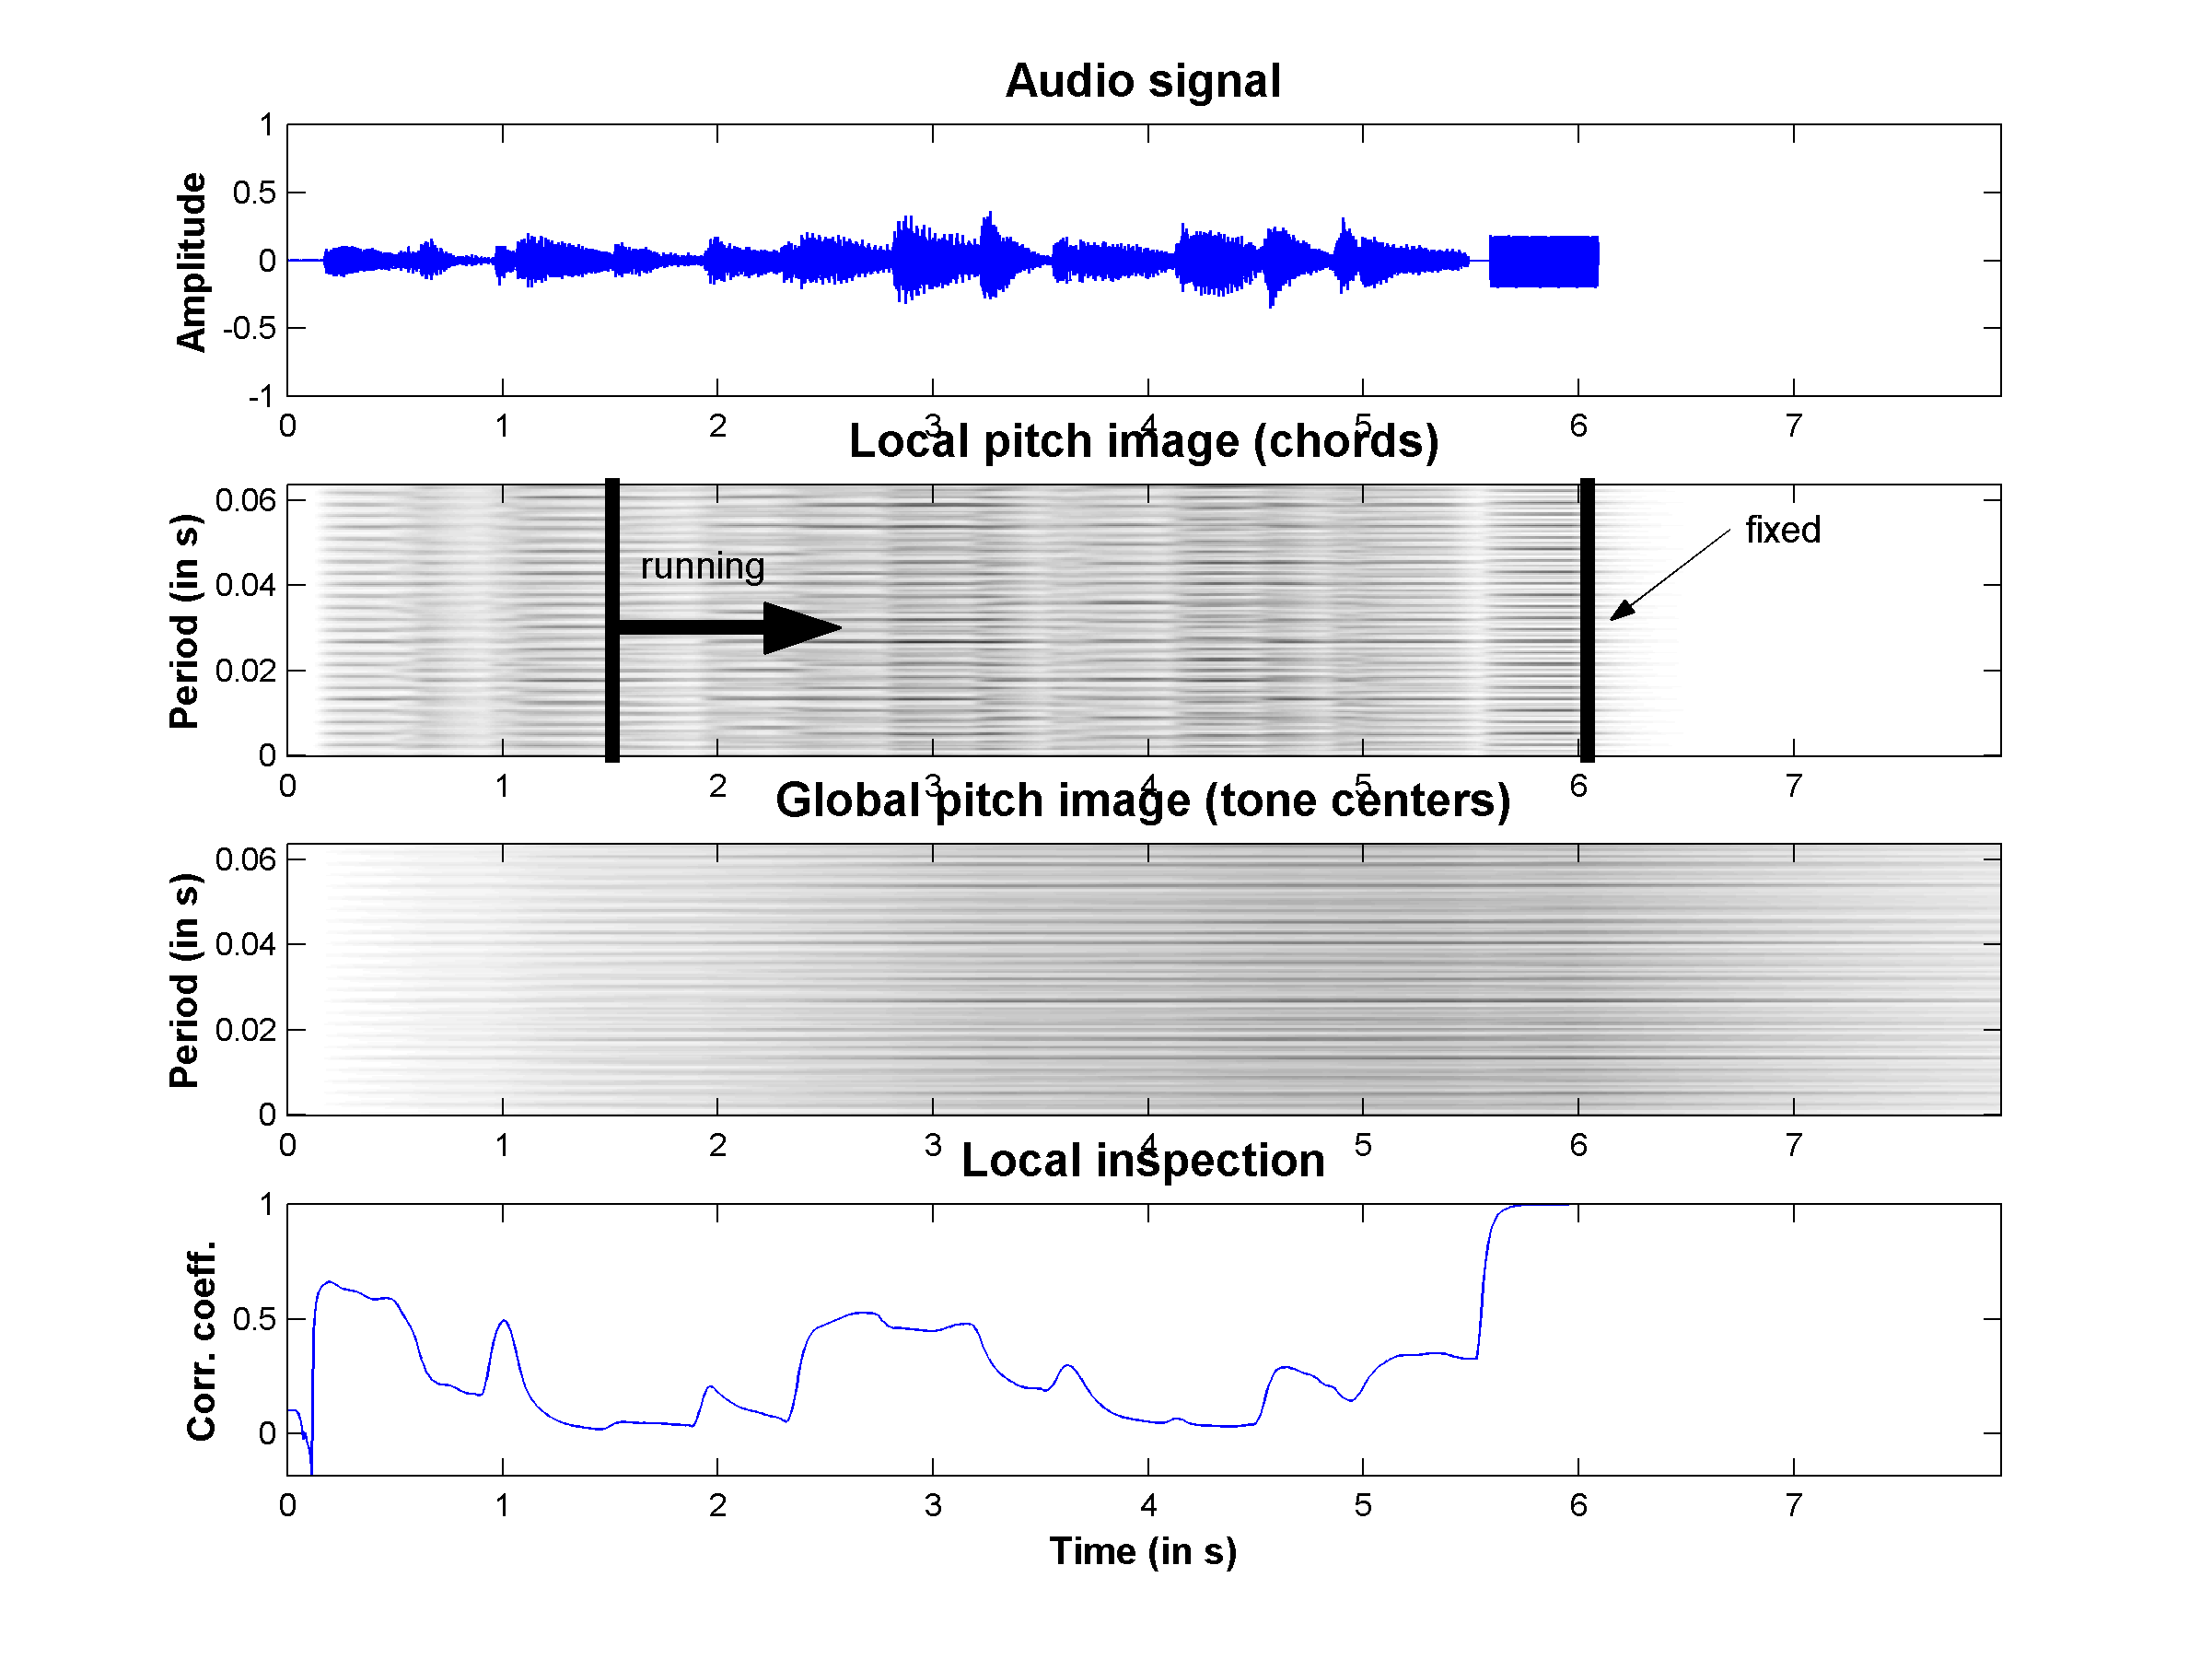
\includegraphics[width=\IPEMDefaultFigureWidth]{Graphics/ContextualityLocalInspection}
    \caption{Inspection of Schumann's Kuriose Geschichte followed
    by a small period of silence and a Shepard probe-tone of
    f$\sharp$. Inspection of local images. From top to bottom:
    audio signal, local pitch image, global pitch image and local
    inspection.} \label{Fig:ContextualityLocalInspection}
\end{figure}

\begin{figure}[h]
    \centering
    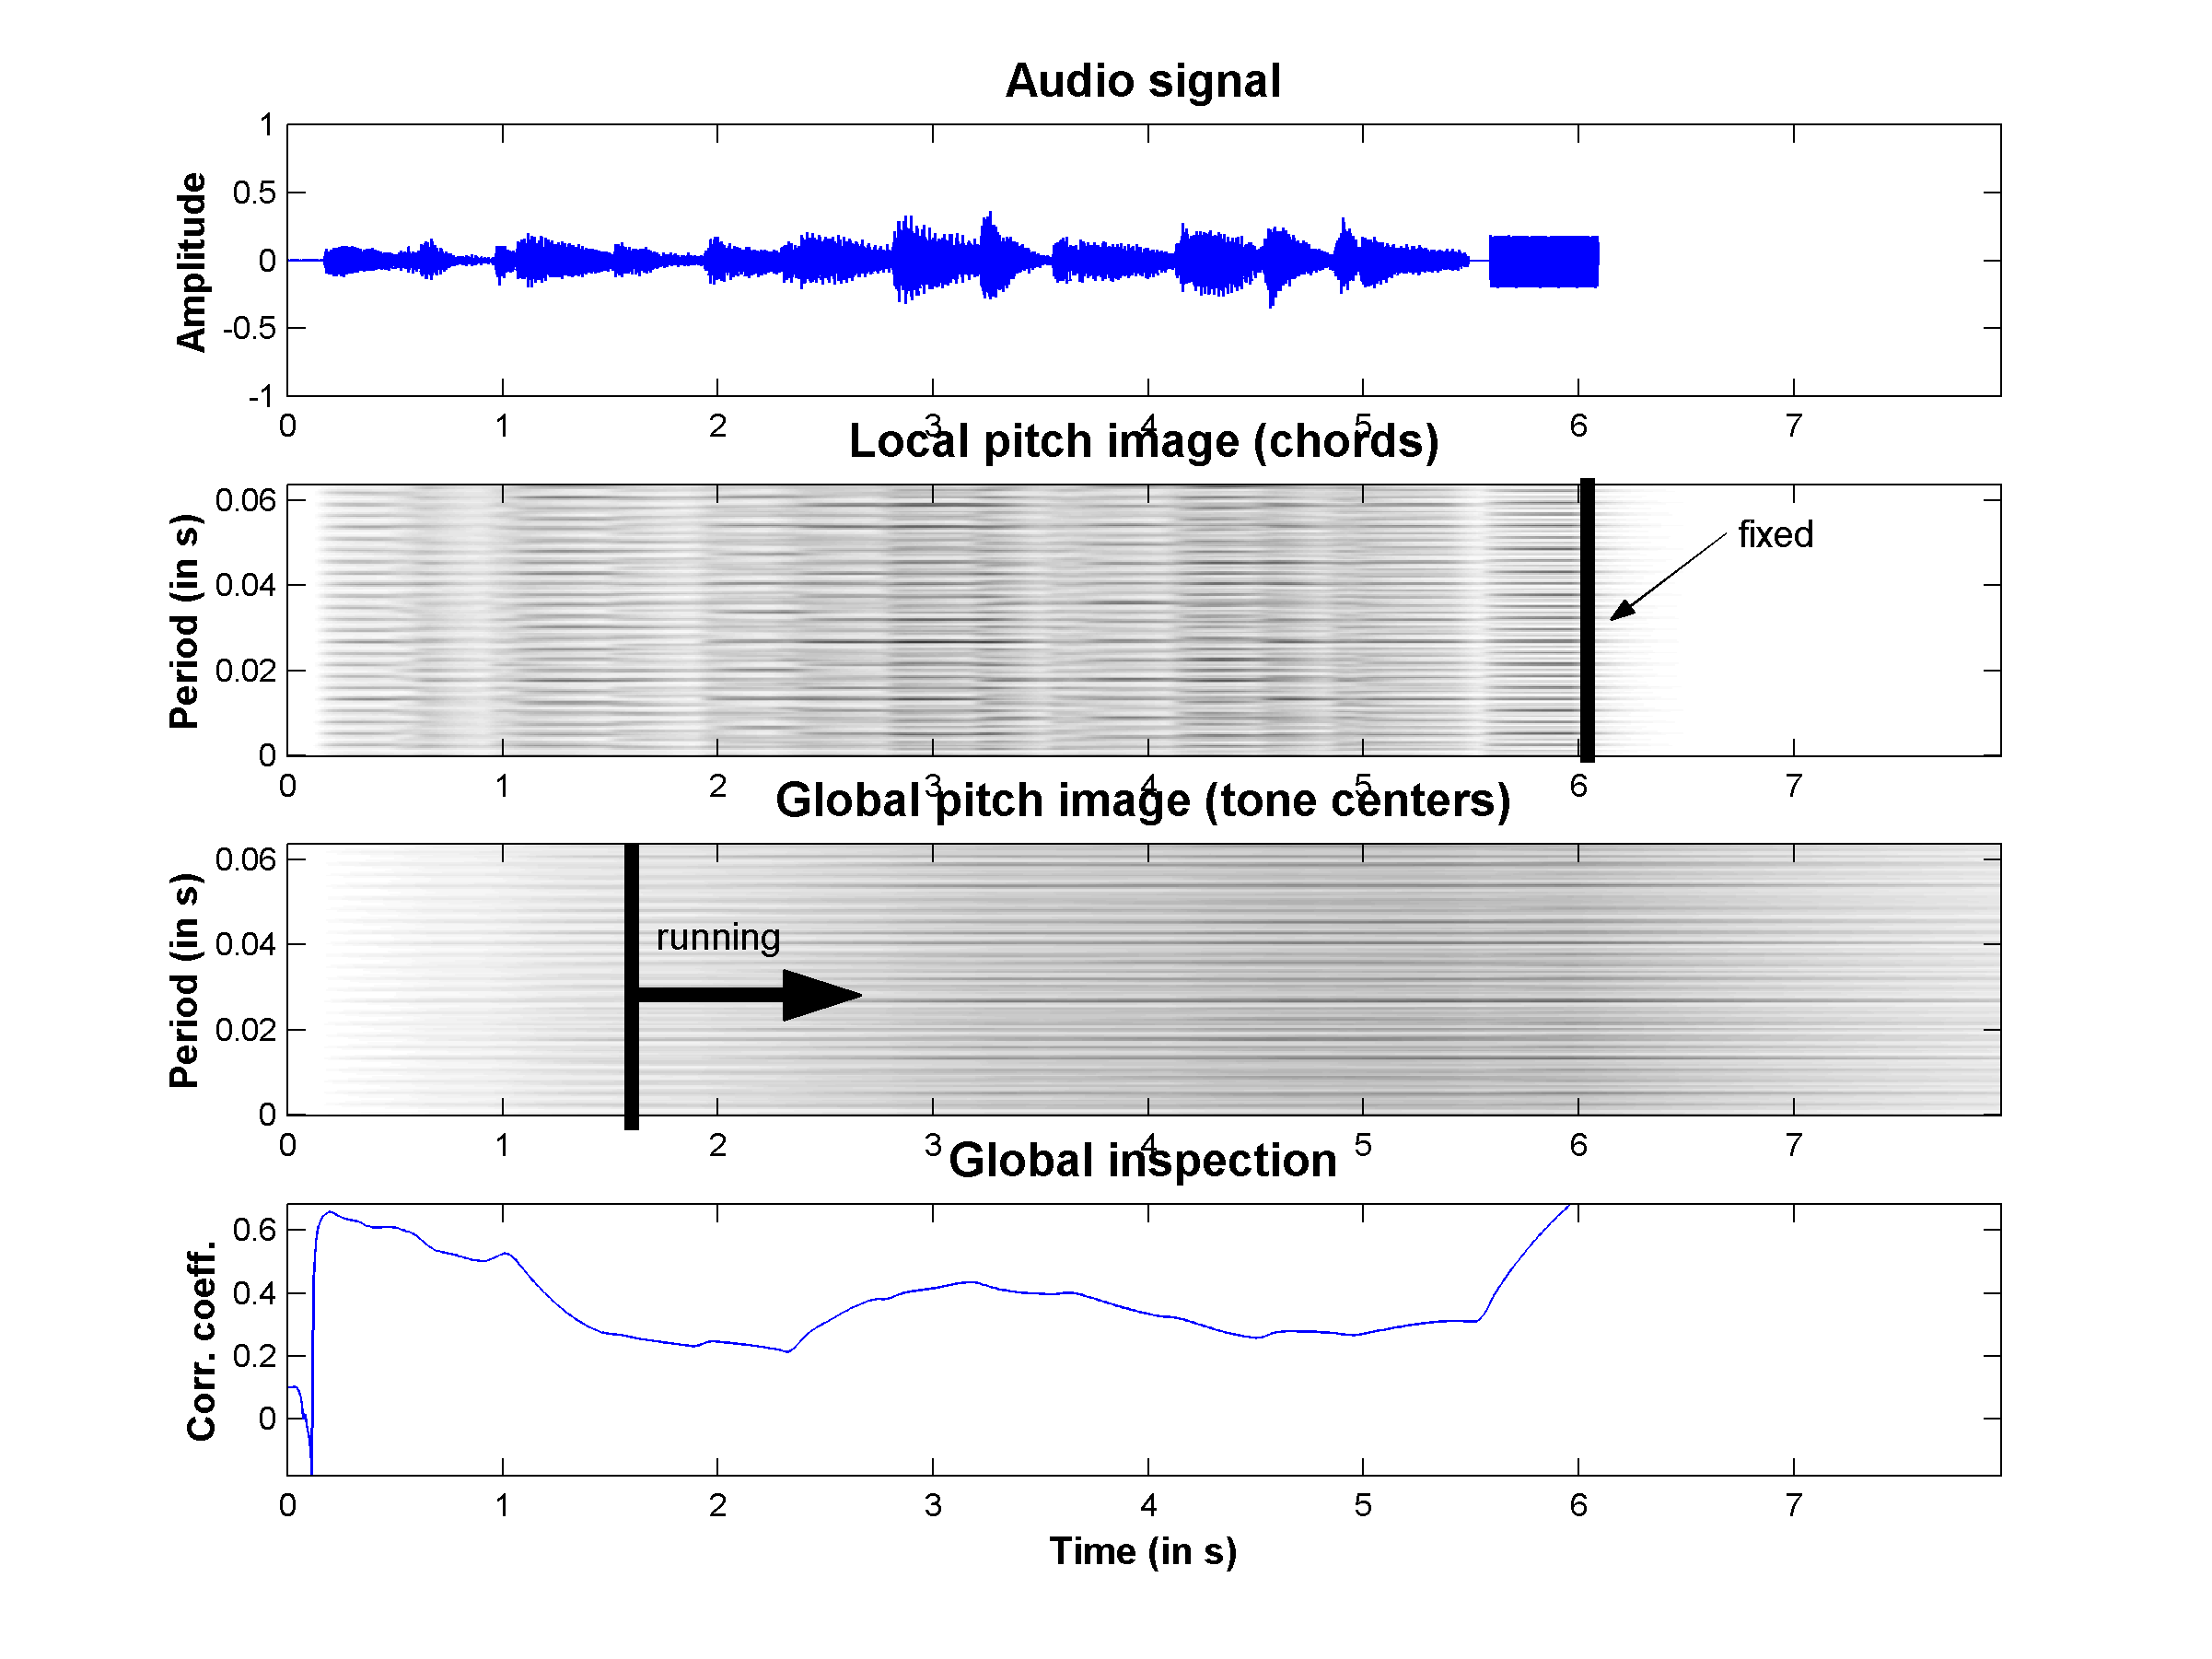
\includegraphics[width=\IPEMDefaultFigureWidth]{Graphics/ContextualityGlobalInspection}
    \caption{Inspection of Schumann's Kuriose Geschichte followed
    by a small period of silence and a Shepard probe-tone of
    f$\sharp$. Inspection of global images. From top to bottom:
    audio signal, local pitch image, global pitch image and global
    inspection} \label{Fig:ContextualityGlobalInspection}
\end{figure}

\begin{figure}[h]
    \centering
    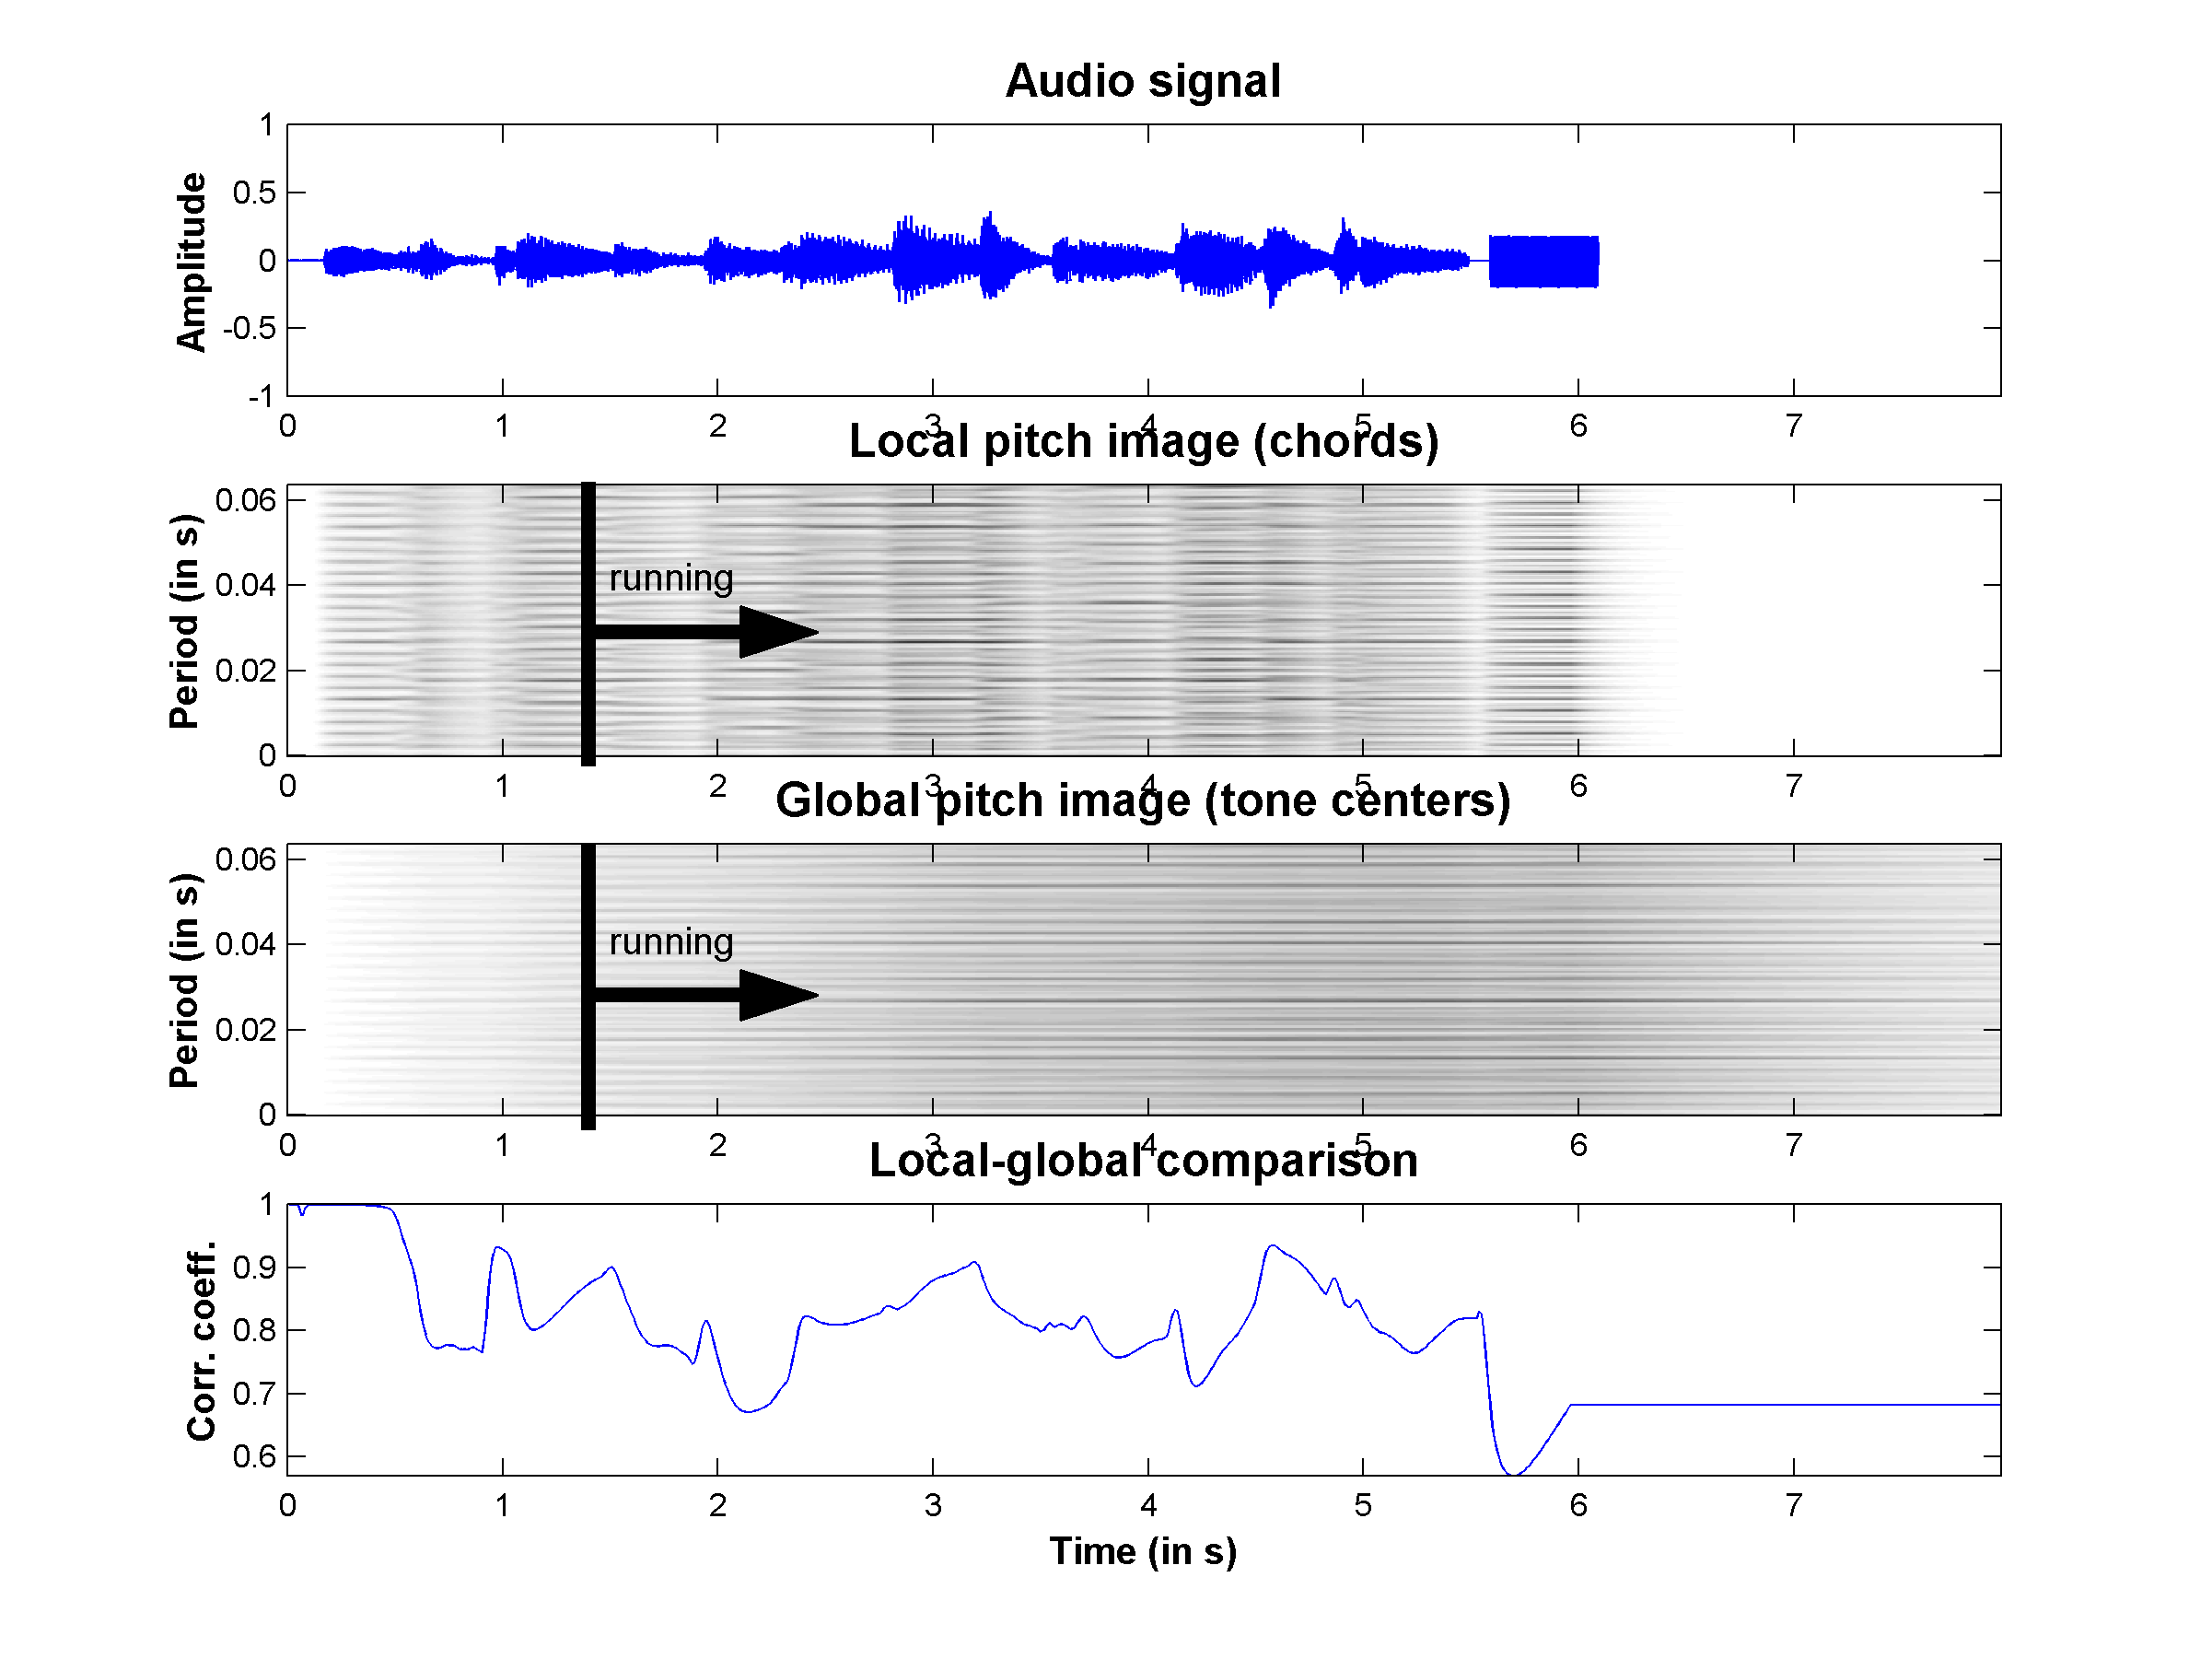
\includegraphics[width=\IPEMDefaultFigureWidth]{Graphics/ContextualityLocalGlobalComparison}
    \caption{Comparison of the local and global pitch images of
    Schumann's Kuriose Geschichte followed by a small period of
    silence and a Shepard probe-tone of f$\sharp$. From top to
    bottom: audio signal, local pitch image, global pitch image
    and comparison between local and global pitch images.}
    \label{Fig:ContextualityLocalGlobalComparison}
\end{figure}

% --------------------------------------------------------------------------------


\newpage
% --------------------------------------------------------------------------------
% Concepts: Experiments
% --------------------------------------------------------------------------------

% ================================================================================
\chapter{Experiments}
\hypertarget{Chapter:ConceptsExperiments}{}
% ================================================================================

% --------------------------------------------------------------------------------
\section{Introduction}
% --------------------------------------------------------------------------------

\IPEMTBC ...Doublecheck this...

Whereas the previous chapter provided a background and description
of the basic modules contained in the IPEM Toolbox, this chapter
focuses on a comparison of the results obtained with our tools
with these obtained from psychoacoustical experiments. Each of the
sections in this chapter contains:
\begin{itemize}
\item a small introduction in which the purpose of the experiment is explained
\item a description of the method that is used
\item a summary of how to run the experiment in practice using
the toolbox and its functions
\item an overview of the obtained results and a discussion thereof
\end{itemize}
The experiments are explained from a conceptual viewpoint, and
each time a link is made between these concepts and the practical
tools (MATLAB functions) available in the toolbox.\\

The following experiments are included:
\begin{itemize}
\item Simulations of roughness in comparison with psychoacoustical data.
\item Short-term model of tonal induction experiments which apply
contextuality to simulate two psychological experiments.
\end{itemize}
Each experiment can be seen as a comparison of one (or more)
module(s) that were handled in the previous chapter with data
obtained from experiments in the psychoacoustic research field.

% --------------------------------------------------------------------------------
% --------------------------------------------------------------------------------
\newpage
\section{Roughness experiments}
% --------------------------------------------------------------------------------

% Make target for following functions:
\hypertarget{Concepts:IPEMRoughnessDemo}{}
\hypertarget{Concepts:IPEMGenerateANIForRoughnessTest}{}
\hypertarget{Concepts:IPEMGenerateANIForScales}{}
\hypertarget{Concepts:IPEMRoughnessRun}{}

\subsection{Introduction}
% --------------------------------------------------------------------------------
The \hyperlink{Concepts:Roughness Module}{Synchronization Index
Model}, which forms the kernel of the Roughness Module (RM), is
based on the idea that roughness depends on the degree in which
neurons synchronize with the beating frequencies. The model
provides a straightforward visualization of the components
contributing to roughness.

In this demonstration the Roughness Module is compared with
behavioral data in psychoacoustics and music psychology. Due due
the fact that a lot of sounds are processed, this demonstration
consumes time and hard disk memory. The output needs about
253MBytes of your hard disk. Performing the full demonstration
takes about 29 minutes on a Windows NT 4.0 system with Pentium
III 600 MHz processor, 256Mb RAM PC130.

% --------------------------------------------------------------------------------
\subsection{Method}
% --------------------------------------------------------------------------------

\IPEMTBC

%\subsubsection*{Framework}
%% --------------------------------------------------------------------------------
%The synchronization index model involves two concepts of
%band-pass filtering:
%\begin{itemize}
%\item
% A concept related to the resonance
%properties of the basilar membrane (=cochlear mechanical
%filtering).
% The width of the band-pass filters that simulate the
%resonance properties simulate the excitation on the basilar
%membrane. The equal width of excitation along the membrane
%corresponds to a quasi-logarithmic relationship in the frequency
%domain. We adopted the Auditory Peripheral Module from Van
%Immerseel and Martens \cite{VanImmerseel:92} but any model of the
%auditory periphery can be used in principle provided that it
%transforms sound into rate-code patterns at the level of the
%auditory nerve. The essential feature of the peripheral model is
%that it introduces the low frequencies in to the spectrum (owing
%to wave rectification).
%\item
%A type of band-pass filtering related to the synchronization of
%neurons to particular frequencies.\
% The upper limit of synchronization in the auditory nerve, which was implemented in
%the Auditory Peripheral Module at 1250 Hz, is clearly too high to
%account for sensory dissonance and roughness. Conceptually,
%synchronization can be divided into three regions corresponding
%to loudness (from 0 to about 25 Hz), to roughness and sensory
%dissonance (from 25 to about 300 HZ), and to pitch (roughly from
%300 to 1250 Hz). The synchronization model has a focus on the
%region between 25 to 300 Hz, which is known to be the frequency
%region of roughness.
%\end{itemize}
%
%The synchronization index model then calculates the roughness by
%a Fourier analysis of the beating frequency range and summing the
%normalized Fourier (magnitude-related) coefficients that
%represent the modulation depth of the beating frequencies. A
%global range for beating frequencies, however, cannot be
%maintained in all auditory channels. In particular, the
%synchronization filtering seems to rely on more narrow band-pass
%filters in the auditory channels whose central frequency is $<$
%800 Hz.


\subsection{Application}
% --------------------------------------------------------------------------------
\subsubsection*{Some Practical Considerations}
% --------------------------------------------------------------------------------
The contents and the functions of the demonstration package for
the roughness experiments can be found in the directory
IPEM$\backslash$Demos$\backslash$Roughness. To perform the
experiments execute the main script
\hyperlink{FuncRef:IPEMRoughnessDemo}{IPEMRoughnessDemo} for
demonstrating the calculation methods of roughness. The function
\hyperlink{FuncRef:IPEMGenerateANIForRoughnessDemo}{IPEMGenerateANIForRoughnessDemo}
generates all the files for the tests contained in the roughness
demo:
\begin{itemize}
\item
\hyperlink{FuncRef:IPEMGenerateANIForRoughnessTest}{IPEMGenerateANIForRoughnessTest}
(IPEMGenerateANIForRoughnessDemo Part I) generates sounds and
auditory nerve images for the psychoacoustical tests. The sounds
and images are further processed with IPEMRoughnessDemo (Part II).

\item
\hyperlink{FuncRef:IPEMGenerateANIForScales}{IPEMGenerateANIForScales}
(IPEMGenerataANIForRoughnessDemo Part II) generates an ANI and
soundfile of several harmonic and inharmonic sounds for the
musical tests.
\end{itemize}

The output, a number of mat-files containing the required auditory
nerve images and the soundfiles, is stored in the directory
RoughnessDemo relative to IPEMRootDir ('output').  The function
\hyperlink{FuncRef:IPEMRoughnessRun}{IPEMRoughnessRun} then calculates roughness of all the specified auditory nerve images using
different models and parameters.

\subsubsection*{Psychoacoustical tests}
% --------------------------------------------------------------------------------
This section compares the model's output with psychoacoustical
data. We start with amplitude modulated signals because they are
characterized by a few parameters whose effect of roughness has
been studied by many authors. We consider the effects of
modulation depth ($m$), amplitude ($A$), carrier frequency
($f_c$), and modulation frequency ($f_m$).

\begin{enumerate}
\item {\textbf{Modulation depth}}
    The dependency of the roughness $R$ on the degree of modulation
    $m$ has been expressed as a power law $R \sim m^n$. Depending on
    the experimental setup, $n$ can slightly vary from $1.2$ up to
    about $2$ \cite{Terhardt:97}. Figure (\IPEMTBC ask Marc)
    \ref{Fig:RoughnessExperimentsModulationDepth} shows the roughness of an amplitude
    modulated tone with $f_c$ 1000 Hz, $f_m$70 Hz, 60 dB in function
    of the modulation depth $m$ linearly increasing from 0 to 1.
    \begin{figure}[h]
        \centering
        
\includegraphics[width=\IPEMDefaultFigureWidth]{Graphics/MissingFigure}
        \caption{Calculated roughness as a function of modulation index $m$ =
        0...1 for a 1000 Hz AM tone}\label{Fig:RoughnessExperimentsModulationDepth}
    \end{figure}
    The dotted line shows the relation $R \sim m^{1.3}$ for $m \leq
    1$. The slope of this curve depends on the parameter $\delta$
    (see Equation \ref{normalizedRoughness}) which was set to 1.5 to obtain
    this result. A change of $\delta$ has a slight effect on the
    slope of the curve in Fig.~\ref{Fig:RoughnessExperimentsModulationDepth}.

\item {\textbf{Amplitude}}
    The effect of amplitude is illustrated in Fig.~\ref{Fig:RoughnessExperiments6}
    using an AM tone with $f_c$ 1000 Hz, $m = 1$, $f_m$ 50 Hz, and a
    linear decrease of SPL dB from 70 to 0. The dynamic range of
    neurons is known to be limited in the order of 30-50 dB. However,
    the large dynamic range of the human auditory system is explained
    by the spread of excitation due to the resonance characteristics
    of the basilar membrane \cite{Smith:88}. The spread of excitation
    is reflected in figure ~\ref{Fig:RoughnessExperiments26}a where a broad excitation
    range can be noticed at a level of 70 dB. This range narrows down
    as the level decreases. In figure ~\ref{Fig:RoughnessExperiments26}b, however, one
    may notice that the excitations contribute to the same frequency
    of 50 Hz. From 70 to about 53 dB the roughness halves.
    \begin{figure}[h]
        \centering
        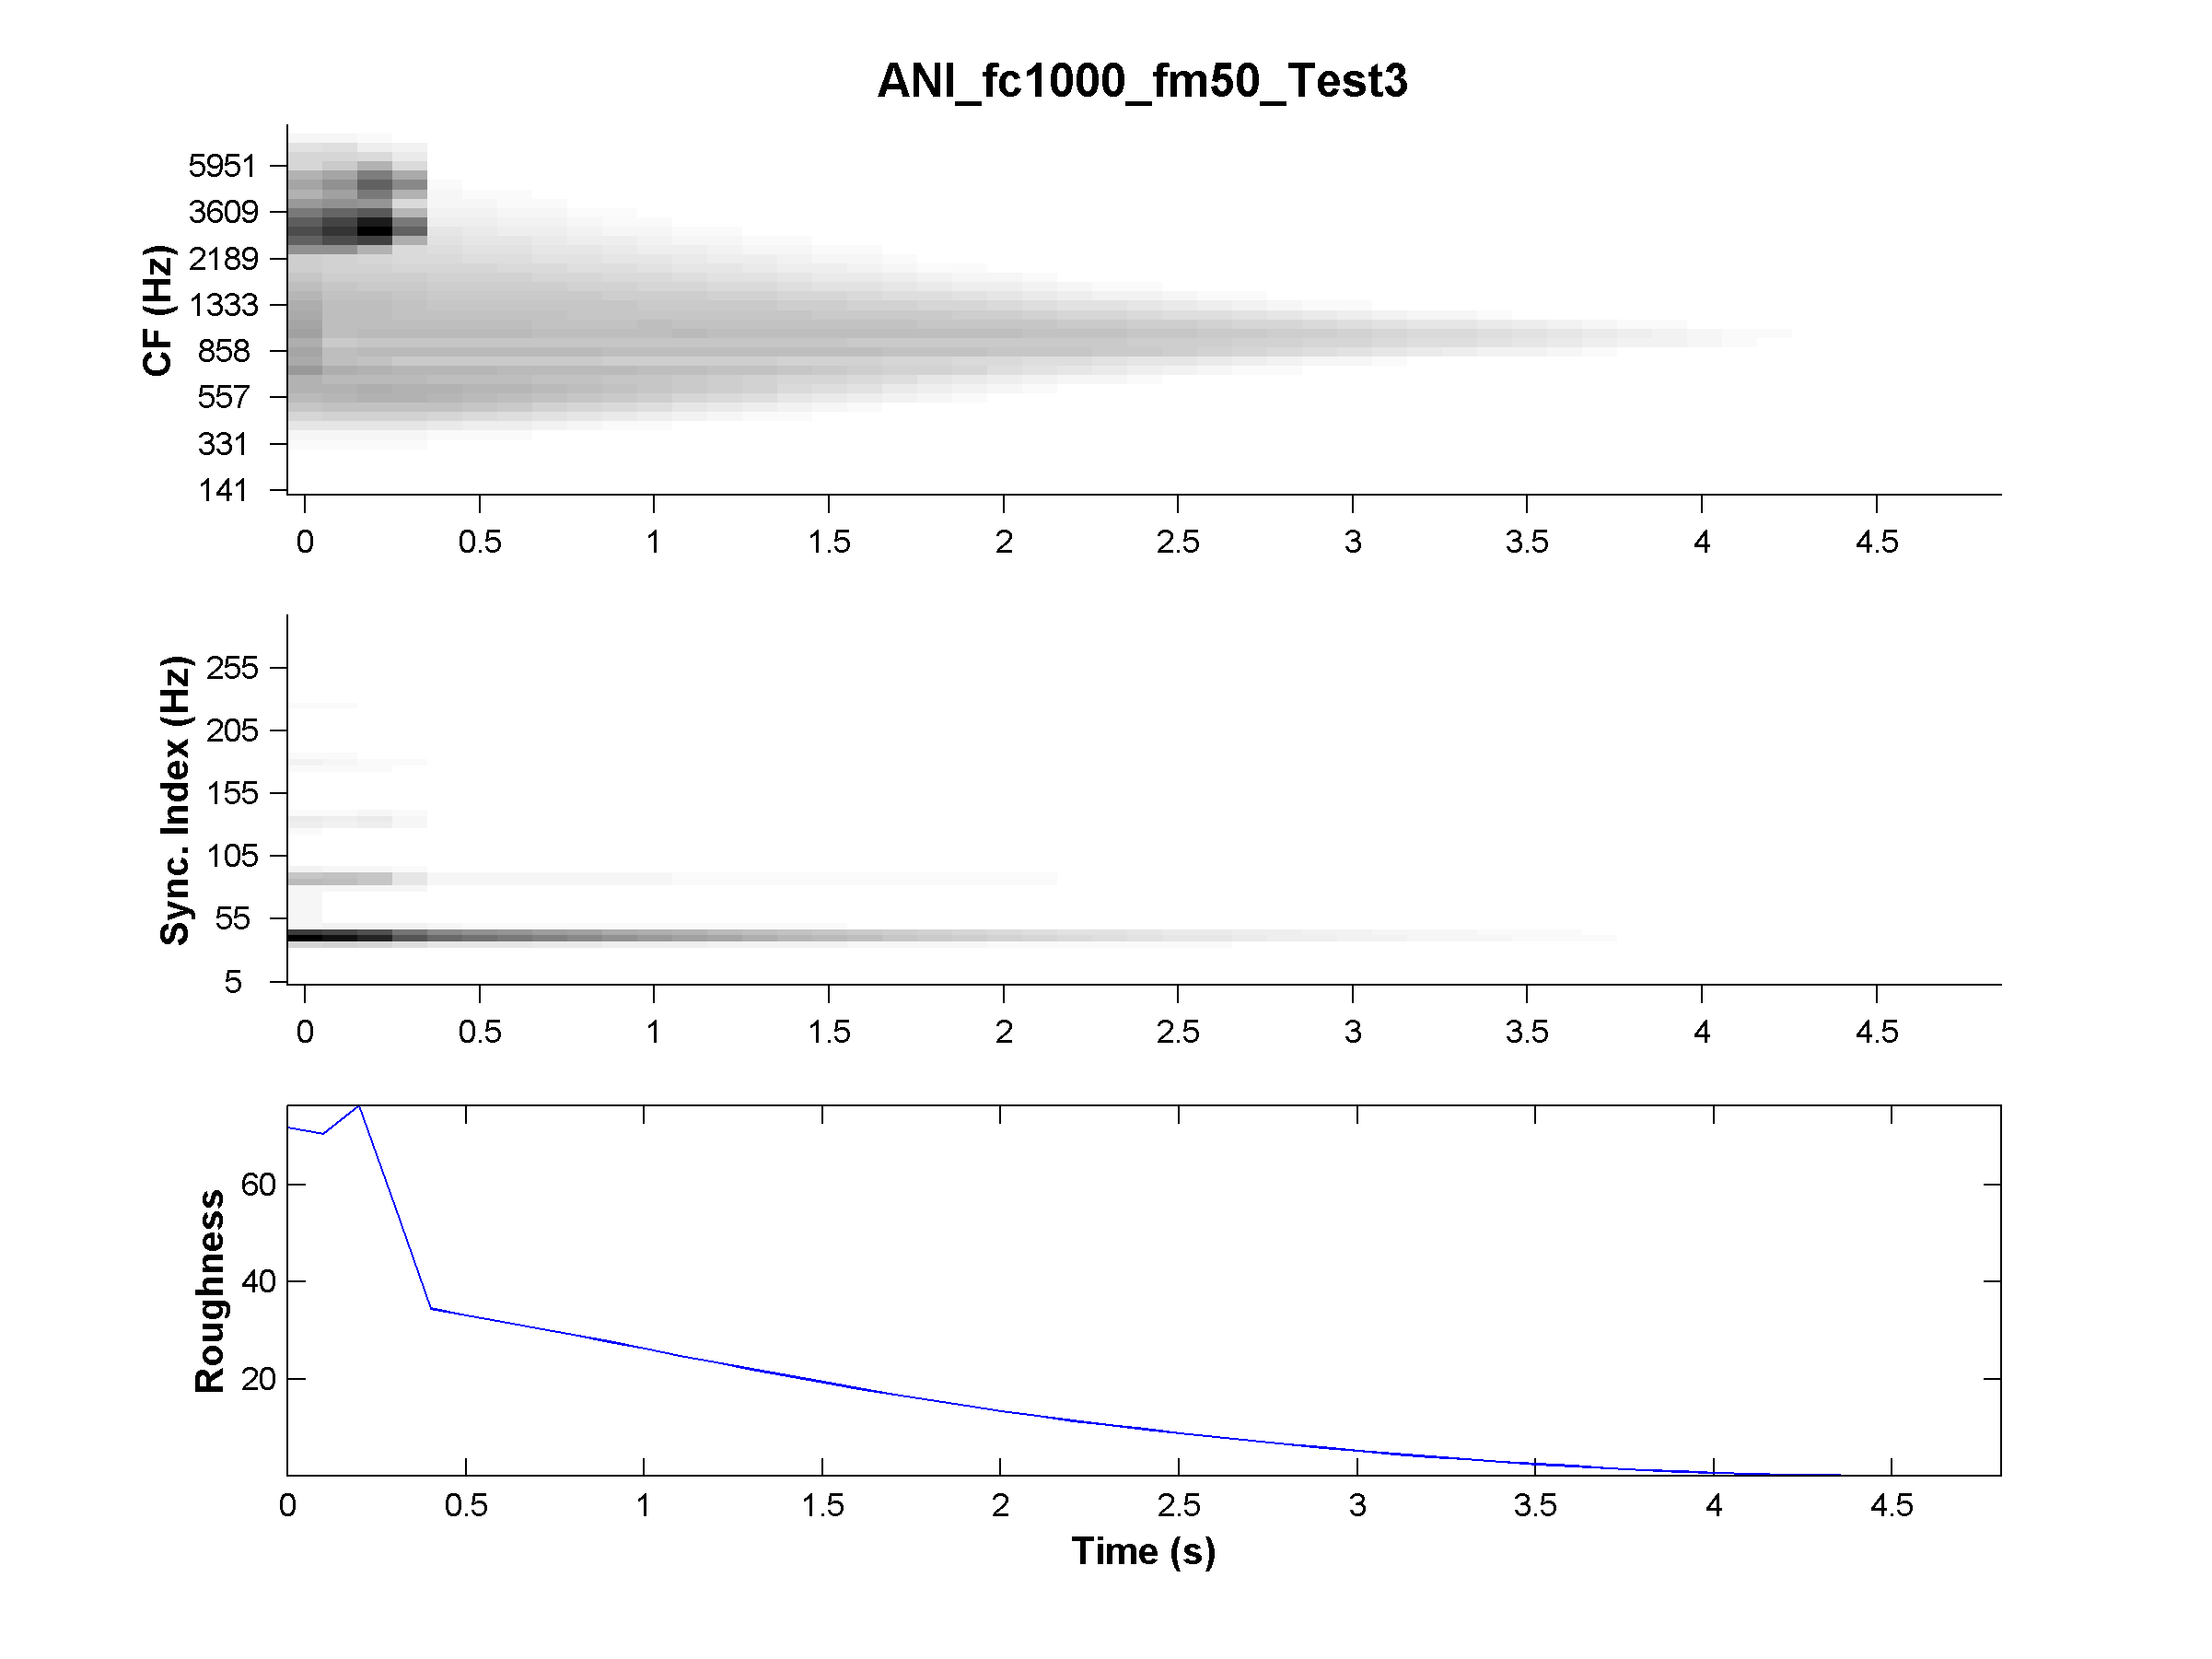
\includegraphics[width=\IPEMDefaultFigureWidth]{Graphics/RoughnessExperiments26}
        \caption{Calculated roughness as a function of amplitude.}
        \label{Fig:RoughnessExperiments26}
    \end{figure}

\item {\textbf{Frequency Modulation}}
    The formula used to calculate an FM tone is
    \cite{DanielWeber:1997}:
    \begin{displaymath}
        s(t) ~=~ \hat{s}.
        sin \left( 2 \pi f_c t - \frac{\Delta f}{f_{mod}}. cos (2 \pi f_{mod} t) \right)
    \end{displaymath}
    where $\hat{s}$ is the effective amplitude. The effects of
    frequency modulation on roughness show a band-pass characteristic
    with maximal values from 40 Hz to 70 Hz \cite{Kemp:1982}
    figure~\ref{Fig:RoughnessExperimentsKemp1}, full line), which our model (dotted line)
    approximates except at $f_{mod}$ 20 Hz, where the estimated
    roughness is clearly too high. The other values fall within the
    quartile range. The signal is
    a 1.6 kHz FM tone at 60 dB with $\Delta f$ 800 Hz whose  roughness
    is measured at $f_{mod}$ 1 10 20 40 60 80 100 200 300 400 500
    Hz.

    \begin{figure}[p]
        \centering
        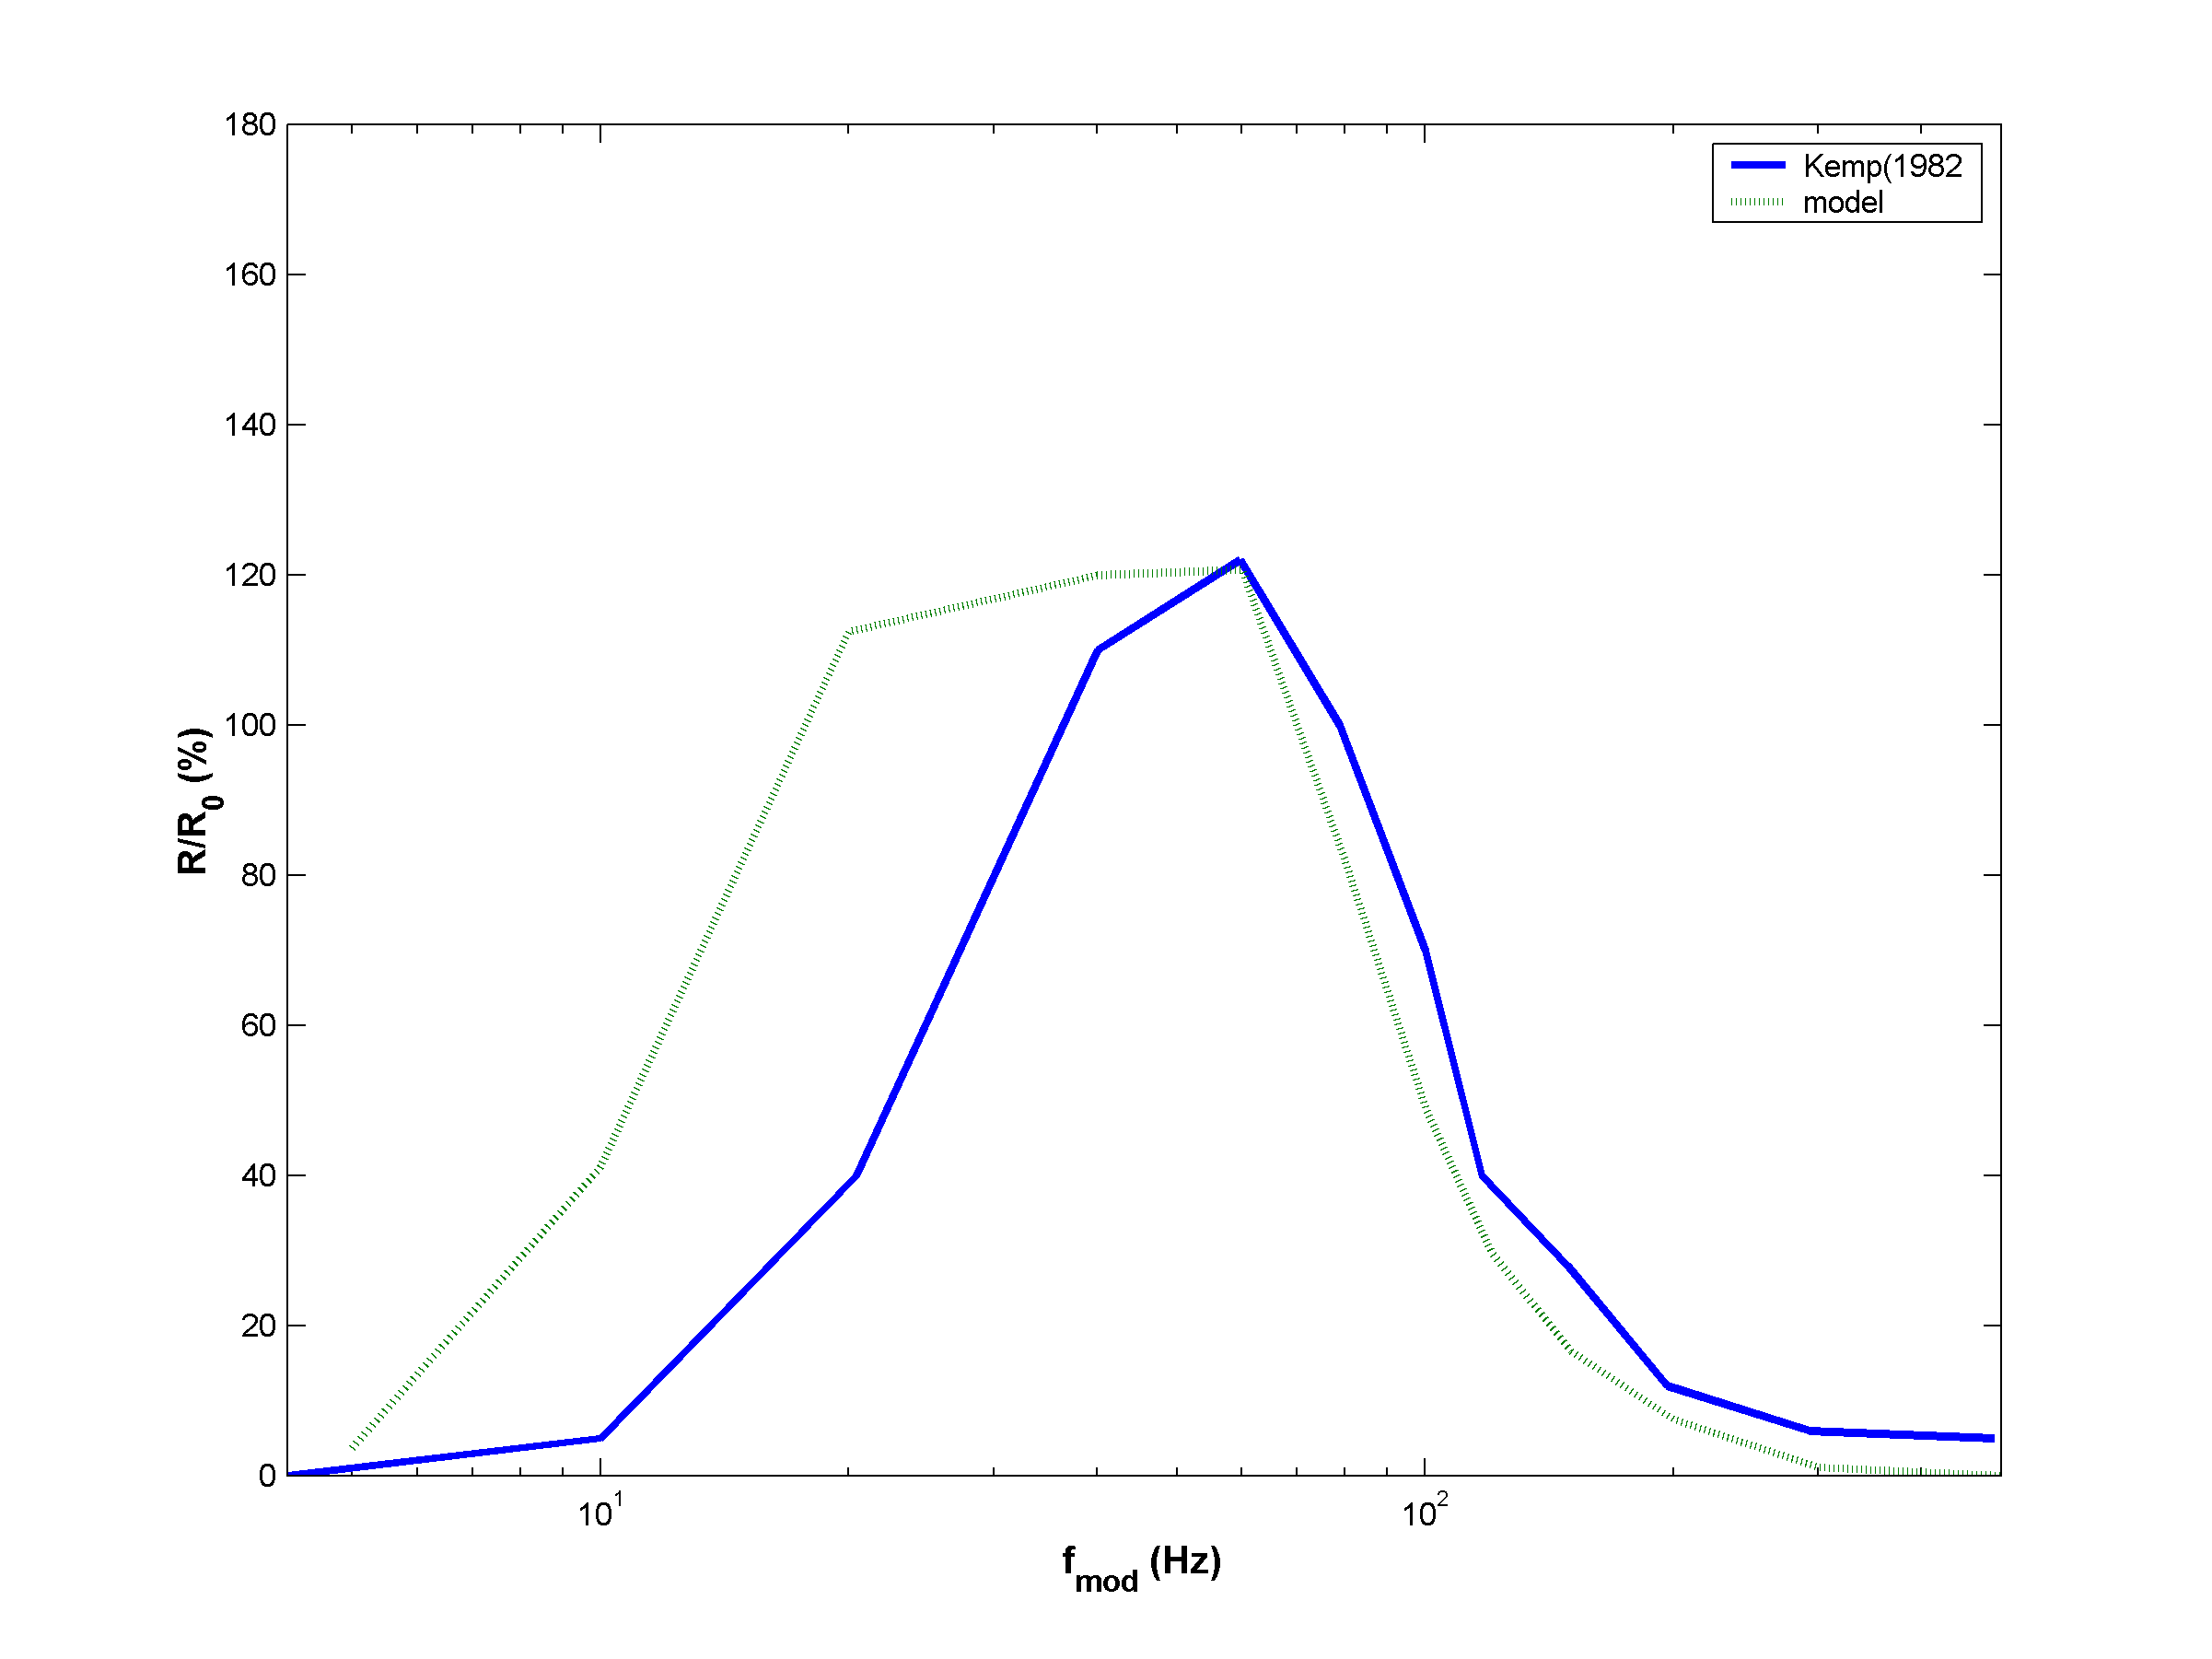
\includegraphics[width=\IPEMDefaultFigureWidth]{Graphics/RoughnessExperimentsKemp1}
        \caption{Calculated roughness as a function of frequency modulation. The signal is
        a 1.6 kHz FM tone at 60 dB with $\Delta f$ = 800 Hz, and $f_{mod}$
        from 1 10 20 40 60 80 100 200 300 400 500 Hz. The peaks are
        generated at the onsets}
        \label{Fig:RoughnessExperimentsKemp1}
    \end{figure}

    In addition, the roughness of a FM tone with $f_c$ 1600 Hz,
    $f_{mod}$ 70 Hz, at 60 dB is measured in function of the frequency
    deviation $\Delta f$ at 10 15 30 60 120 160 340 580 880 1130 1400
    1580 1720 Hz (figure ~\ref{Fig:RoughnessExperimentsKemp2}). The results correspond
    rather well with the available psychoacoustical data, as shown in
    figure ~\ref{Fig:RoughnessExperimentsKemp1}. (All values fall within the quartile
    range).
    \begin{figure}[p]
        \centering
        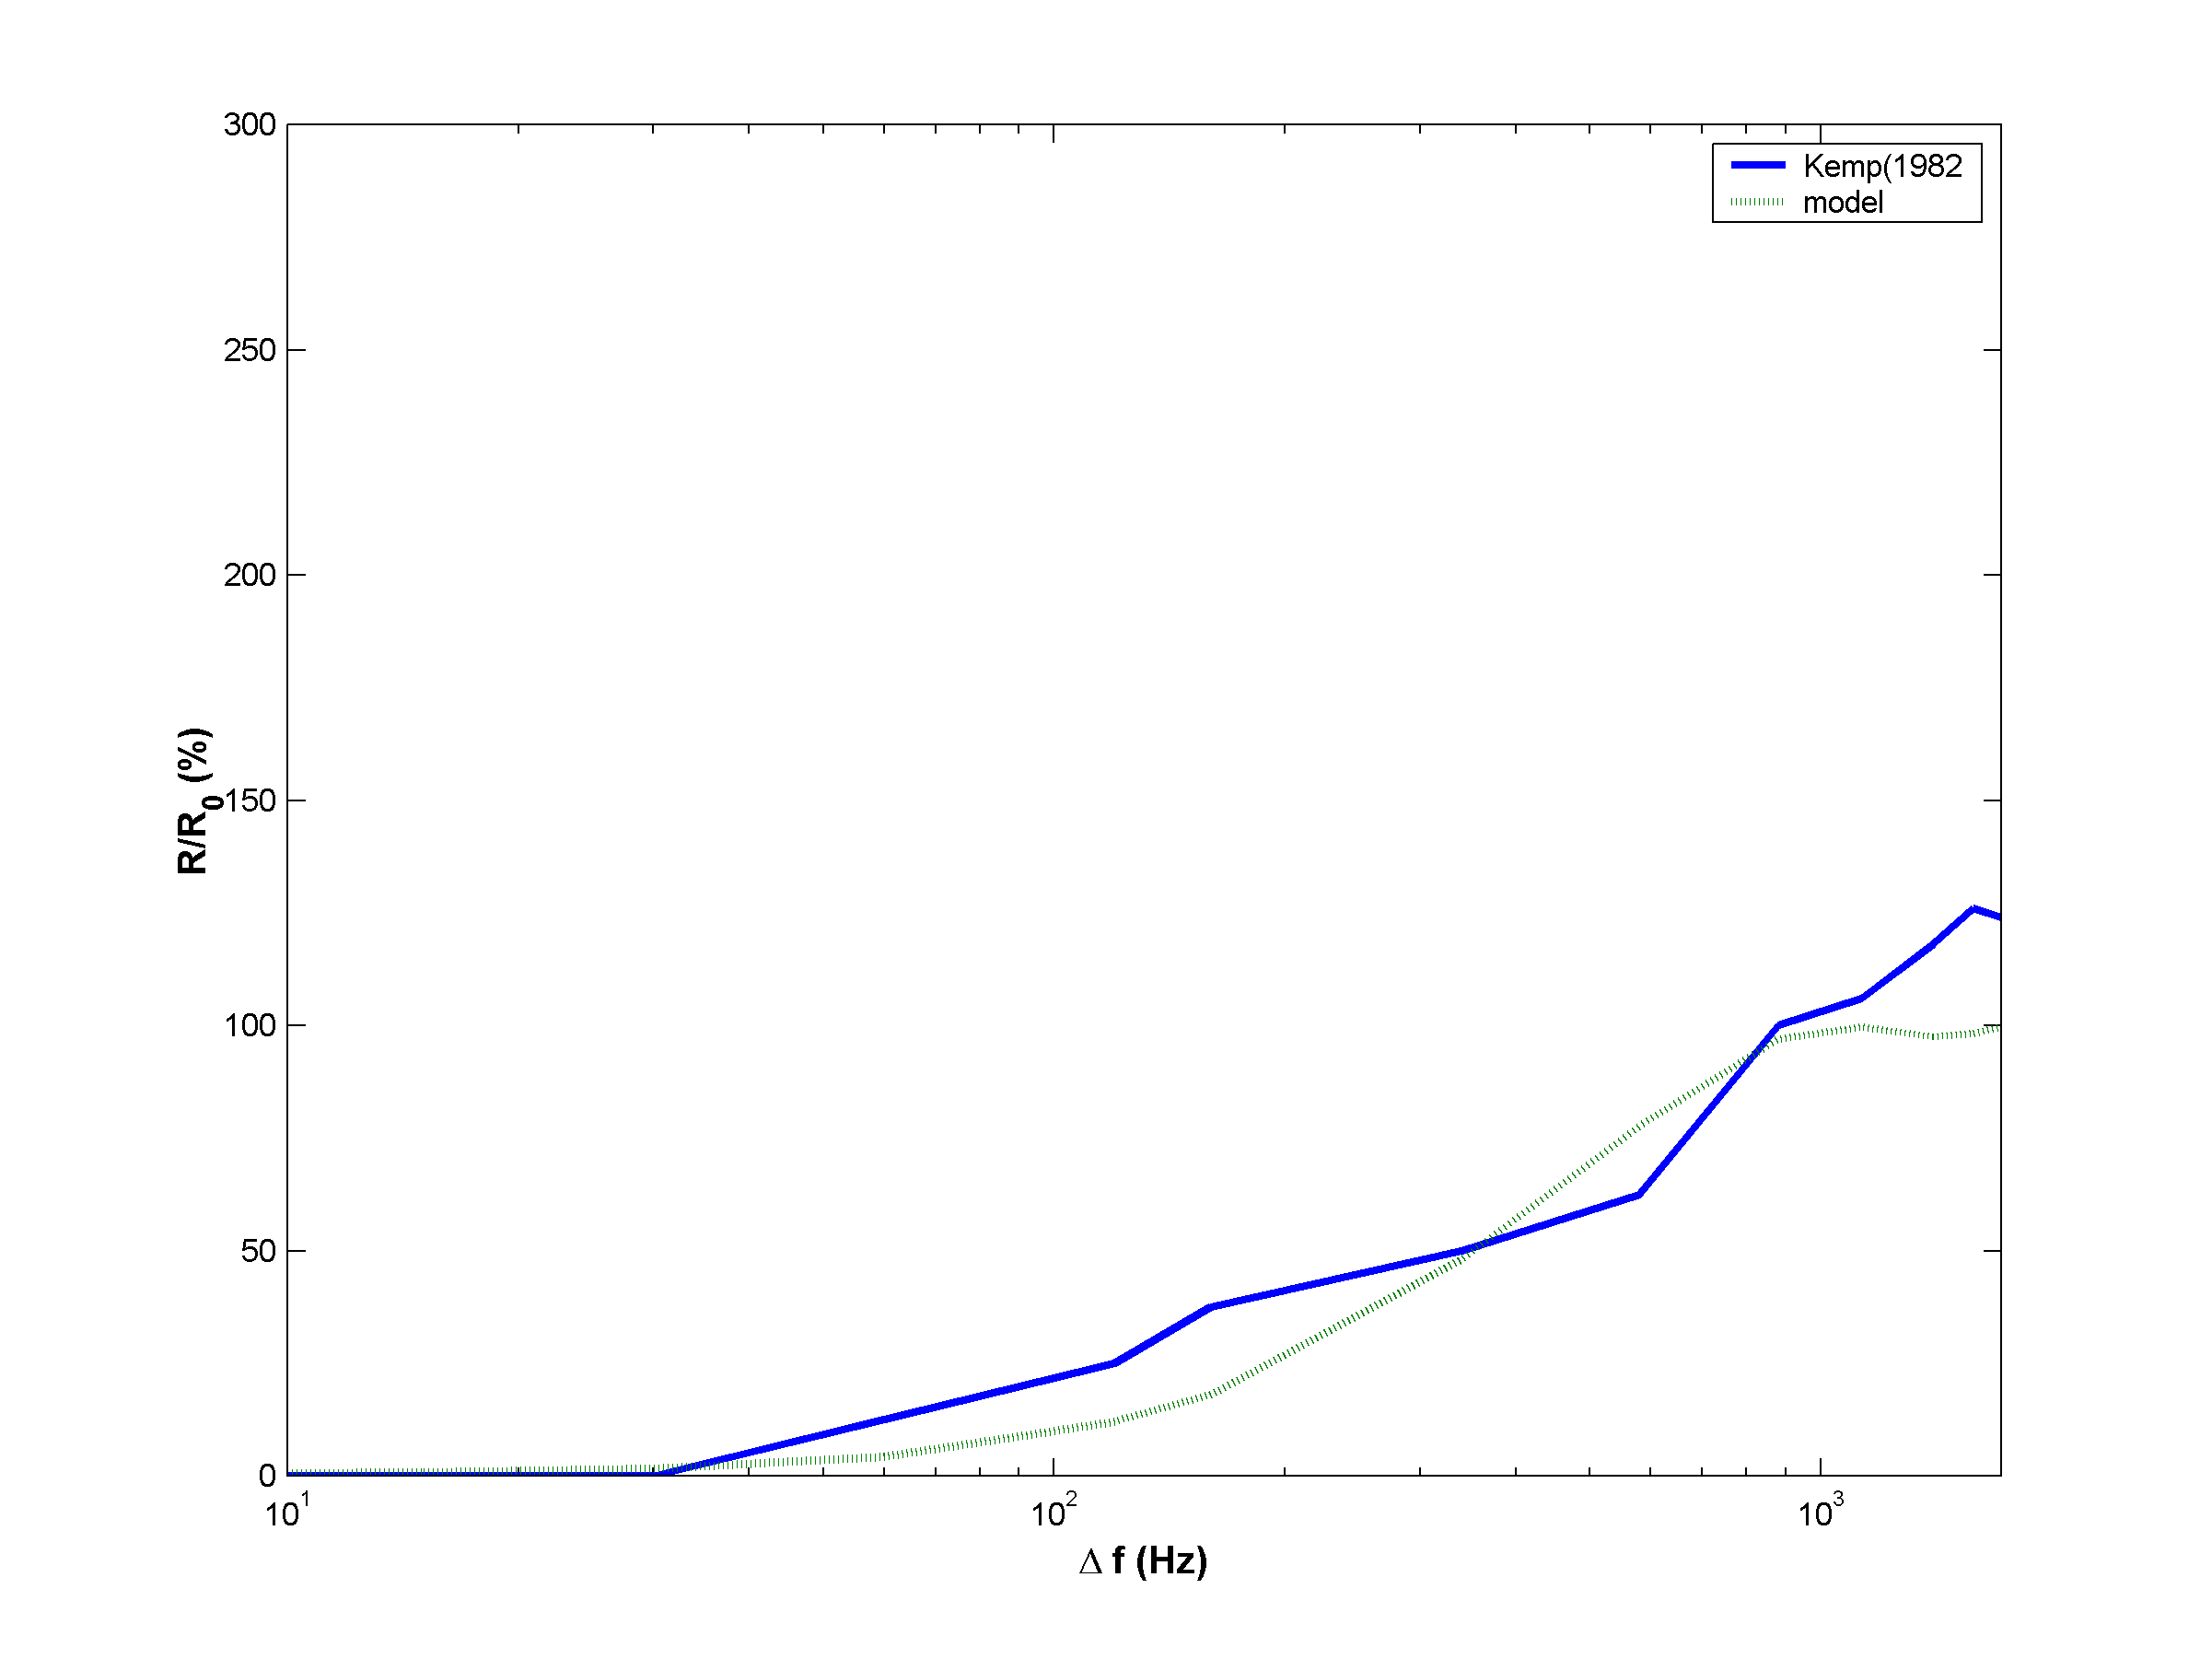
\includegraphics[width=\IPEMDefaultFigureWidth]{Graphics/RoughnessExperimentsKemp2}
        \caption{Comparison of the model's output (dotted line) with
        psychoacoustical data (full line). The signal is
        a 1.6 kHz FM tone at 60 dB with $\Delta f$ 800 Hz measured
        at $f_{mod}$ from 1 10 20 40 60 80 100 200 300 400 500
        Hz.}
        \label{Fig:RoughnessExperimentsKemp2}
    \end{figure}

\end{enumerate}

\subsubsection*{Musical tests}
% --------------------------------------------------------------------------------
The music theoretical interest of the concept of roughness is
demonstrated by taking a harmonic tone complex and playing it
together with a pitch shifted version thus specifying different
musical intervals of the timbre over a defined range. As an
illustration, we took a harmonic tone complex consisting of a
fundamental ($f_0$) at 500 Hz and 5 harmonics with equal
amplitude. This tone is played together with a pitch shifted copy.
The shift over 5 seconds is linear in frequency up to the upper
octave ($f_0$ 1000 Hz). The roughness as calculated with the
synchronization index model is shown in figure
~\ref{Fig:RoughnessExperiments31}.
\begin{figure}[p]
  \centering
  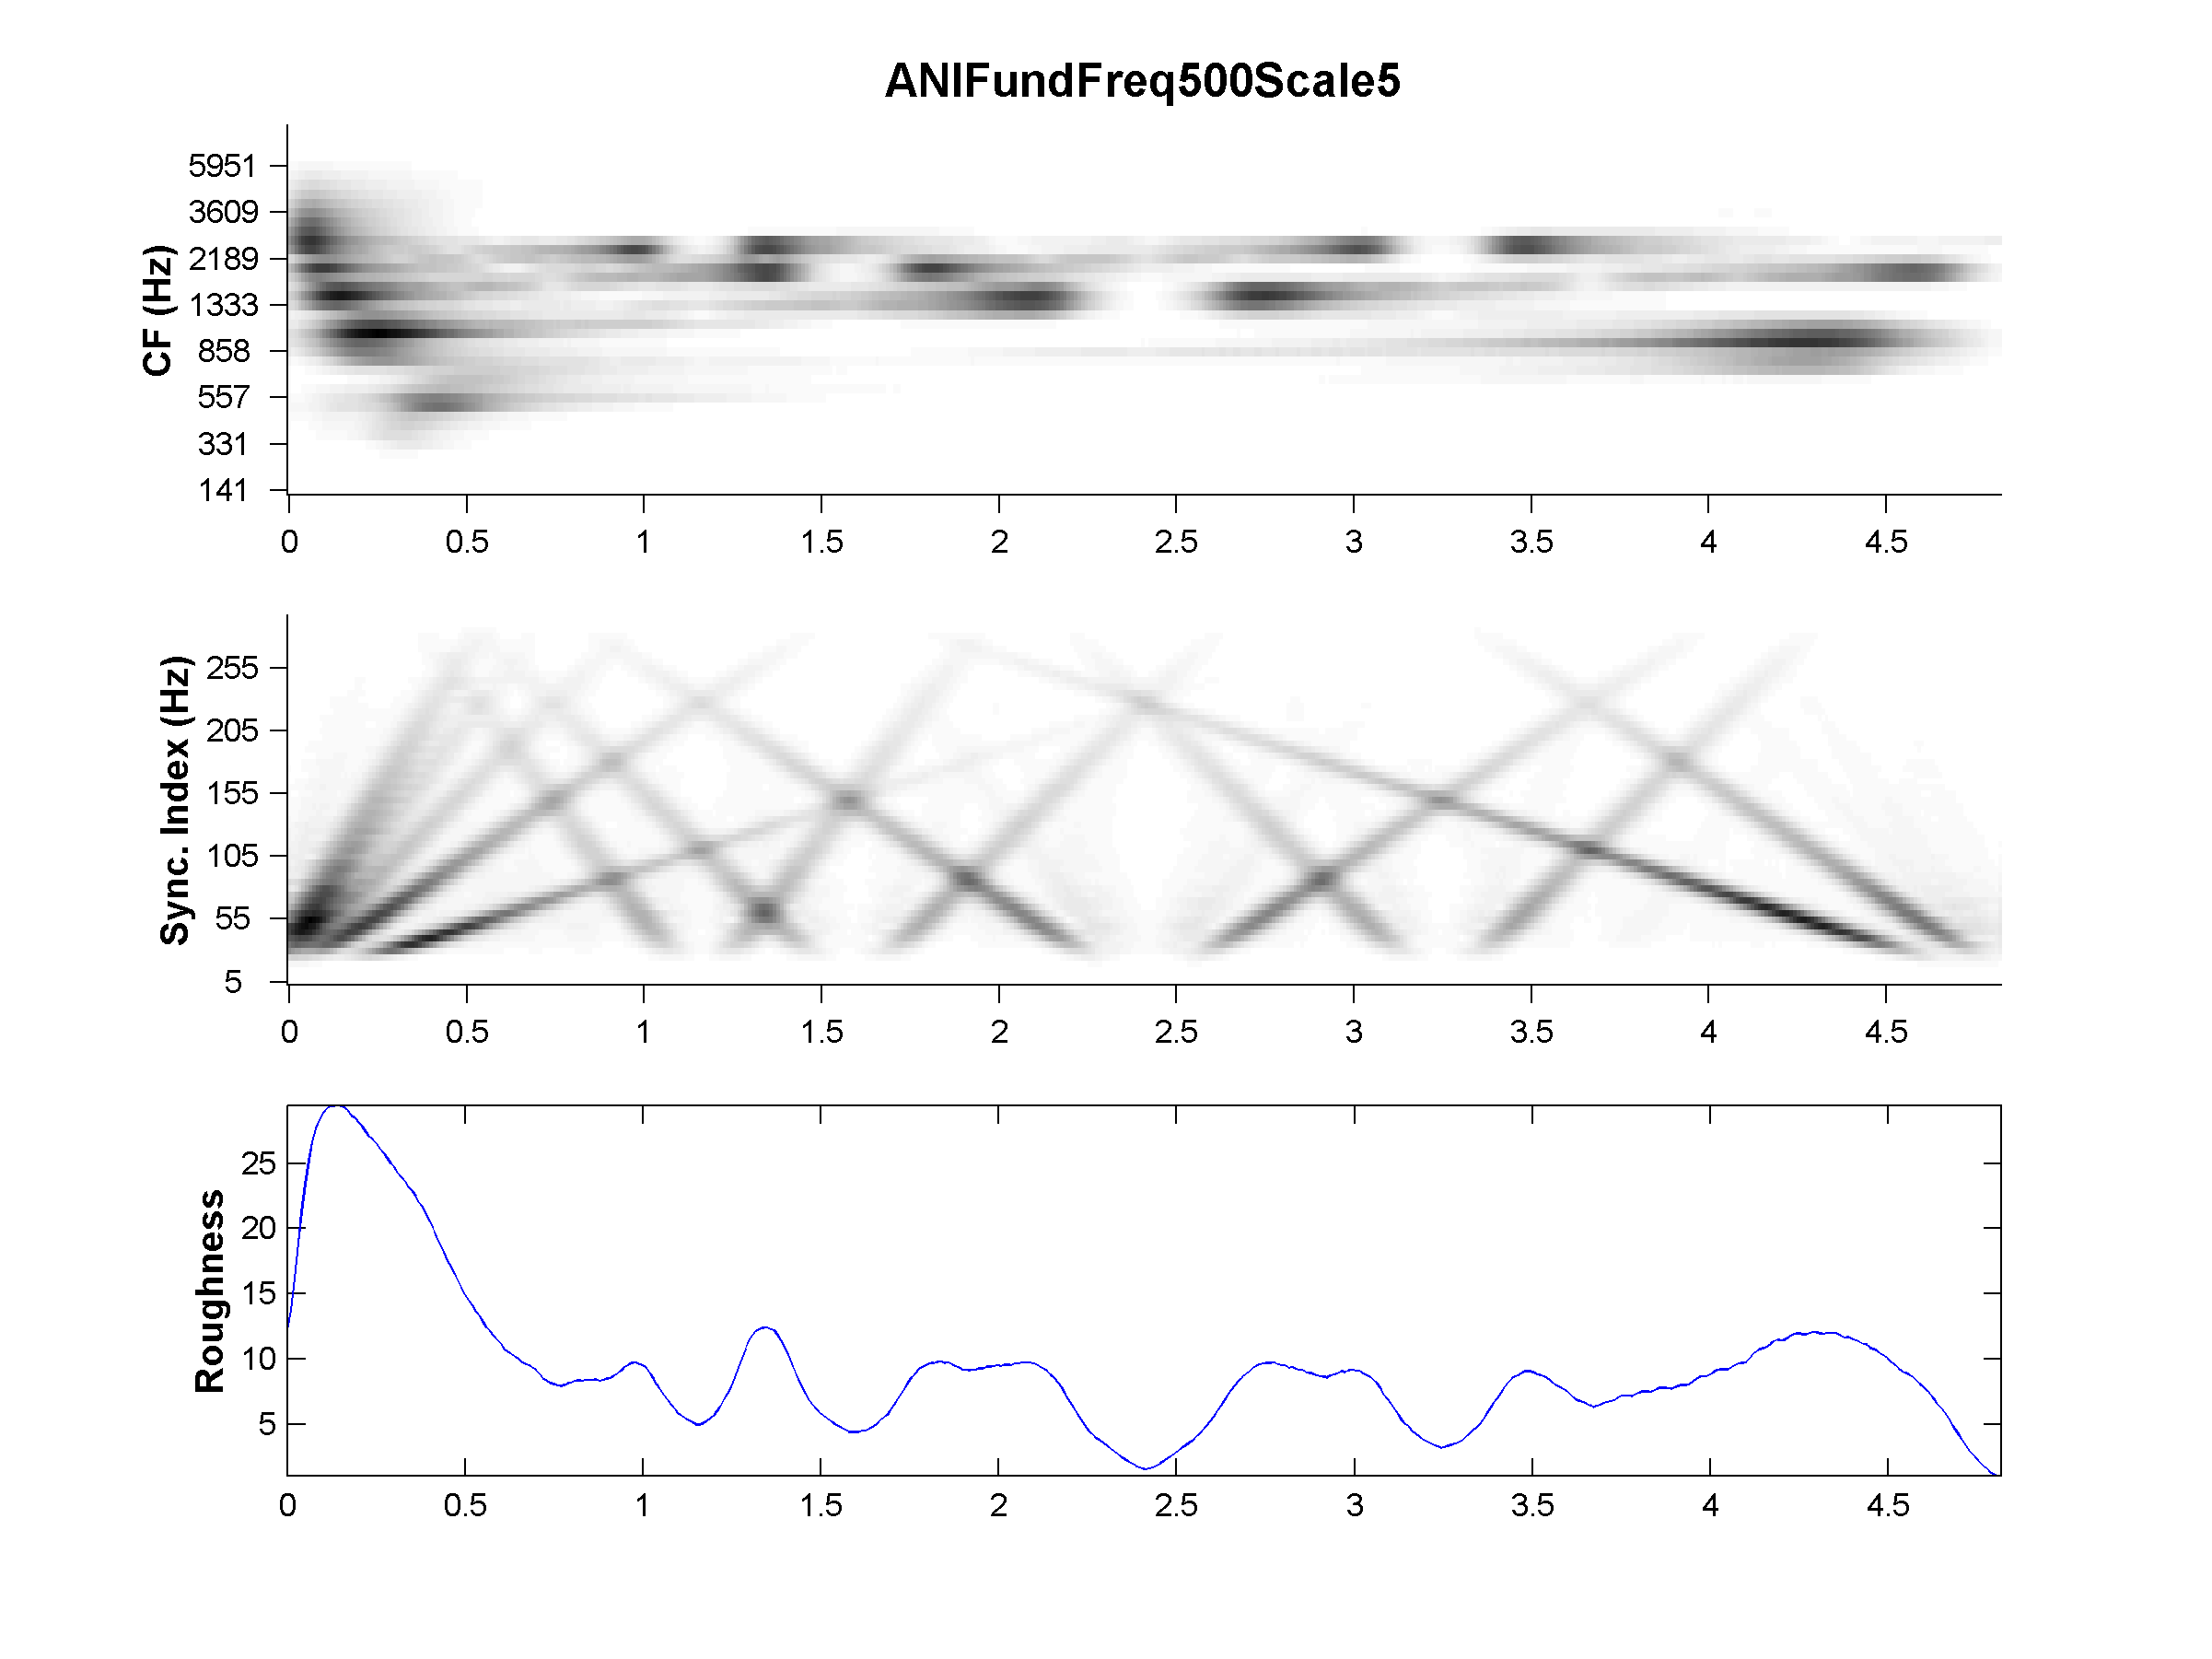
\includegraphics[width=\IPEMDefaultFigureWidth]{Graphics/RoughnessExperiments31}
  \caption{A harmonic tone complex with $f_0$ 500 Hz is played together with a
  pitch shifted copy (up to $f_0$ 1000 Hz). The harmonics have equal amplitudes.
  Top panel: excitation in the auditory channels.  Middle panel: synchronization
  index.
  Lower panel: roughness as calculated with the synchronization index model.}
  \label{Fig:RoughnessExperiments31}
\end{figure}

The roughness curve in figure ~\ref{Fig:RoughnessExperiments31}
can be compared with the results of the curve-mapping model of
roughness of \citeA{Sethares:98}(figure
~\ref{Fig:RoughnessExperiments30}). This model takes the
frequency-amplitude values as input (no sound!) and calculates the
curve using the psychoacoustical curve of \citeA{Plomp}. The
Synchronization Index Model (figure
~\ref{Fig:RoughnessExperiments33}), apart from its good agreement
with this theoretical model, provides an additional cue in showing
the 'spectral' (=excitation in the auditory channels) as well as
'temporal' (=synchronization index profile) factors that
contribute to roughness. Note that the dips are less deep than in
Sethares' model, which is partly due to the fact that the model
works on a glissando of harmonic tone complexes, rather than on
separate intervals. The points of minimal roughness indicate a
hierarchical order of intervals in terms of roughness. This
hierarchy can be musically exploited as the points of minimum
roughness may indicate candidates for a musical scale.

\begin{figure}
    \centering
    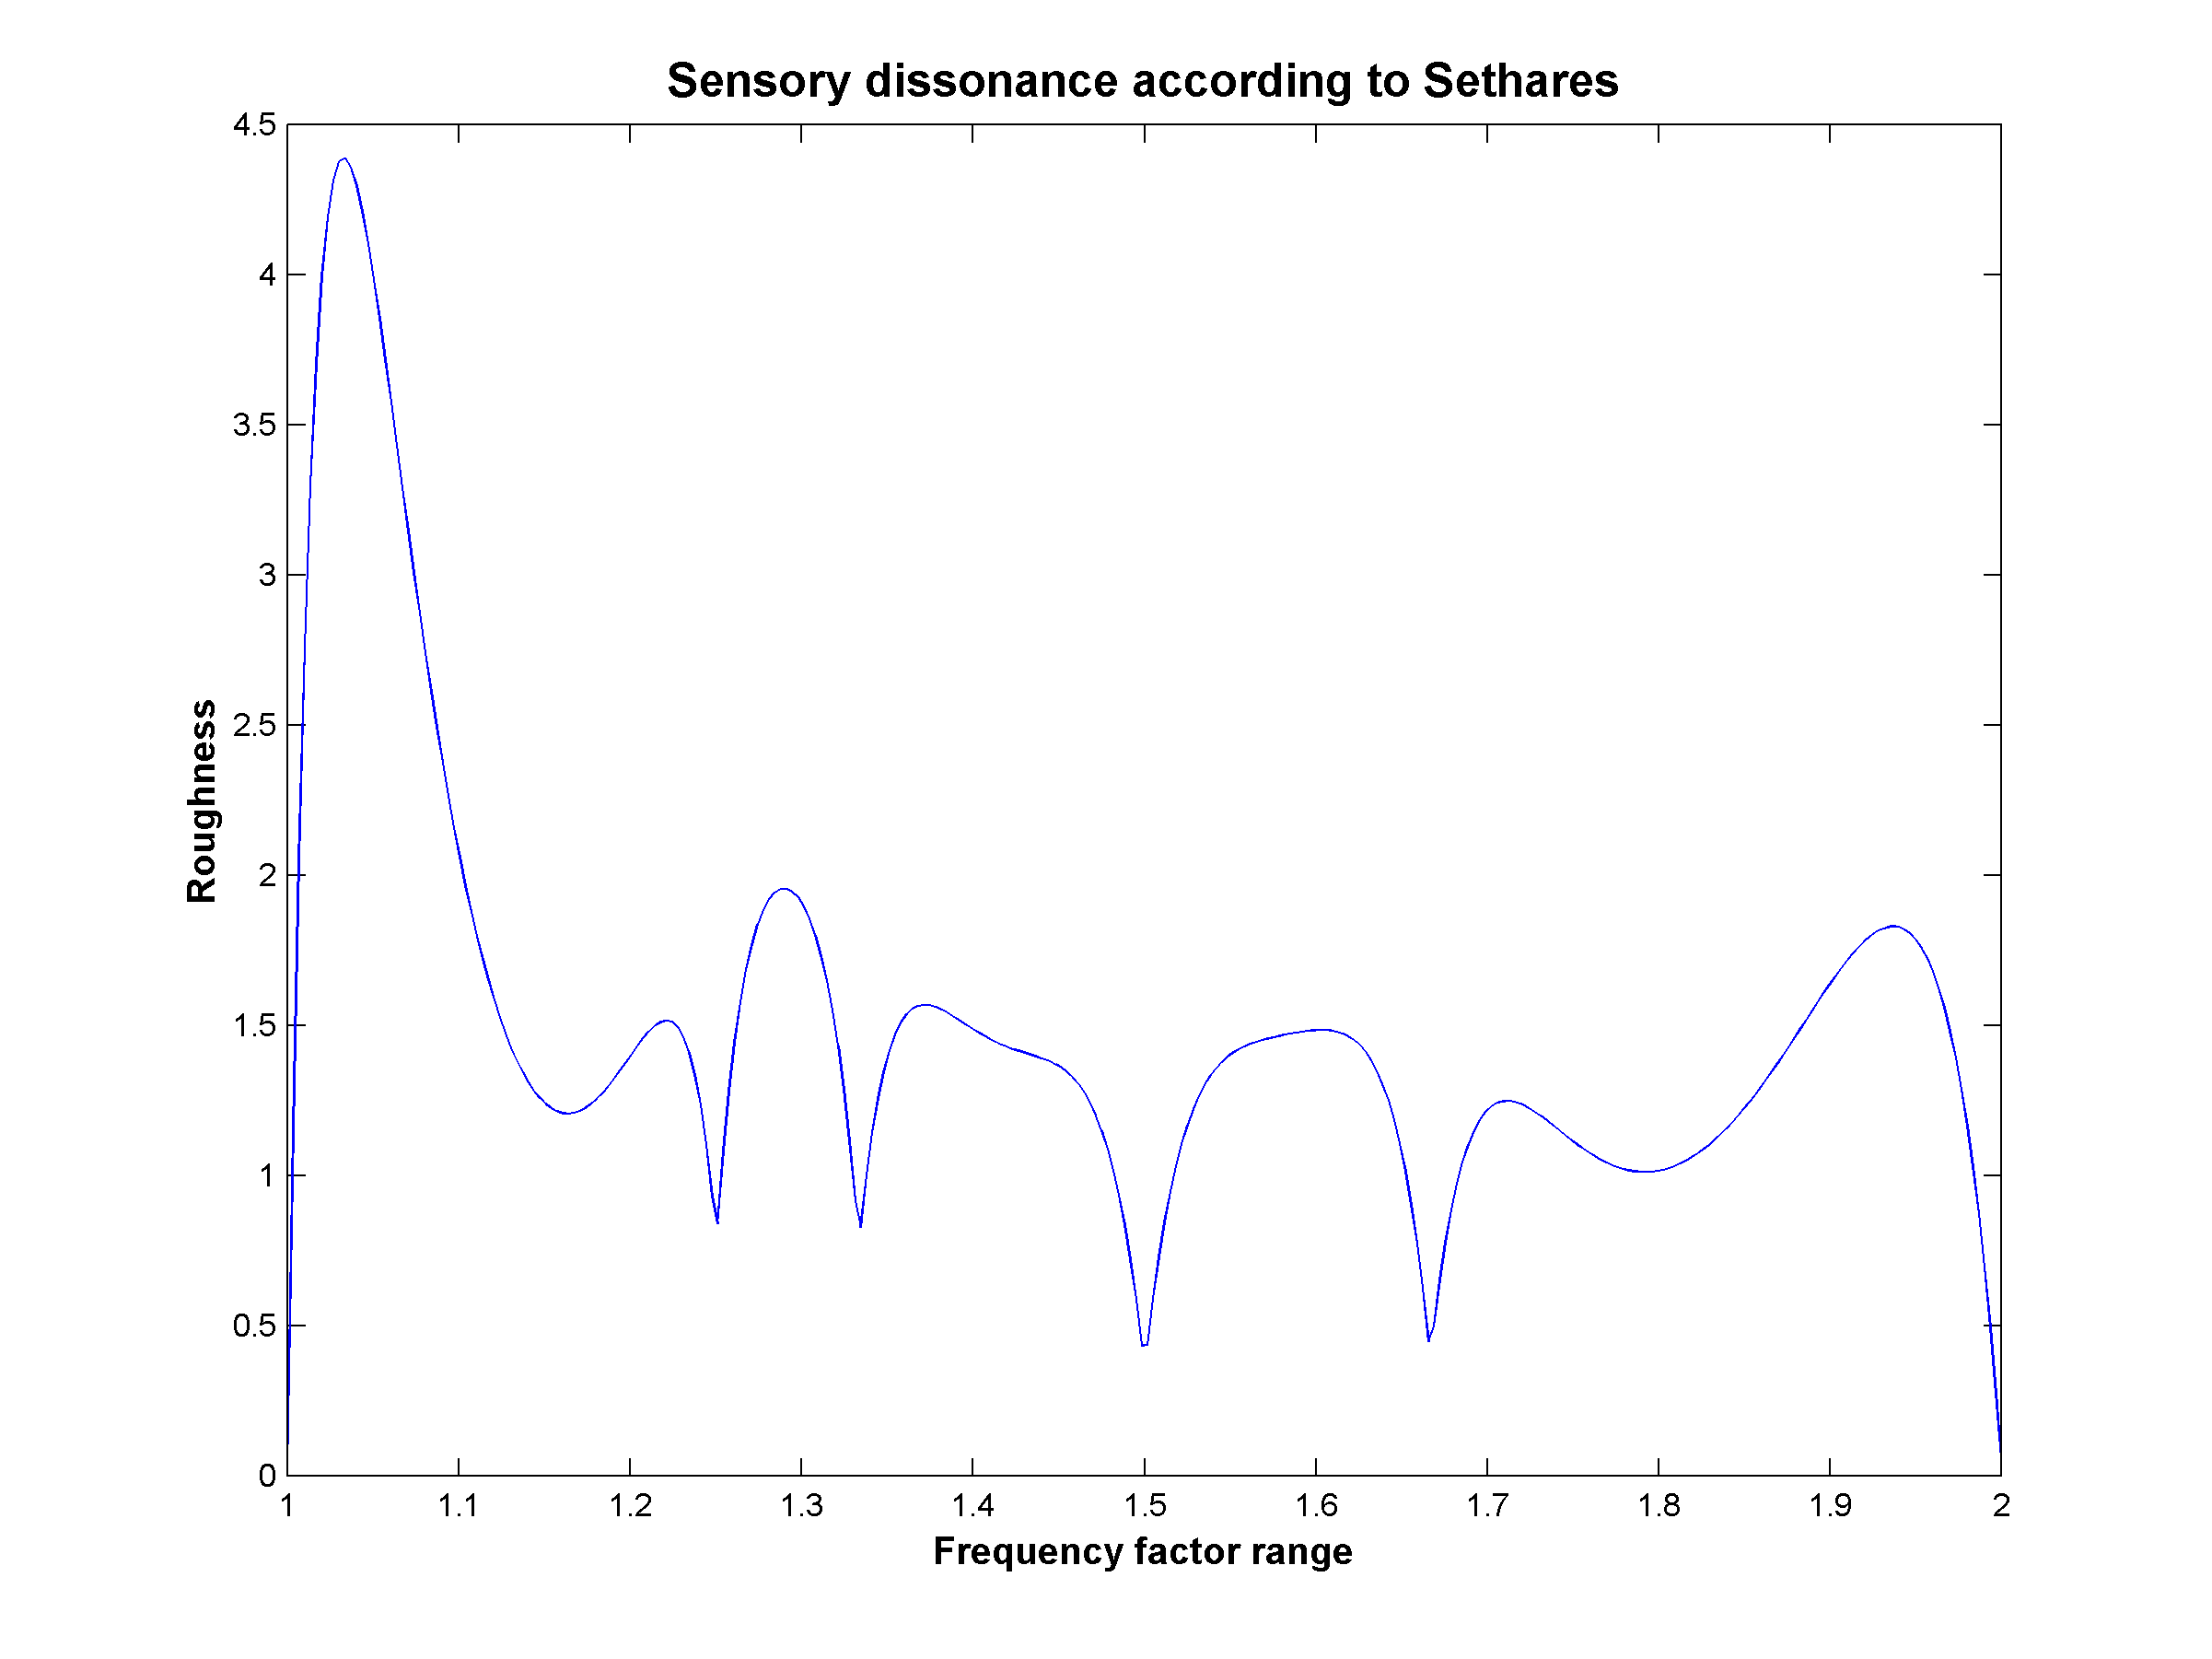
\includegraphics[width=\IPEMDefaultFigureWidth]{Graphics/RoughnessExperiments30}
    \caption{Sensory
    dissonance as calculated with the curve-mapping model of Sethares}
    \label{Fig:RoughnessExperiments30}
\end{figure}

\begin{figure}
    \centering
    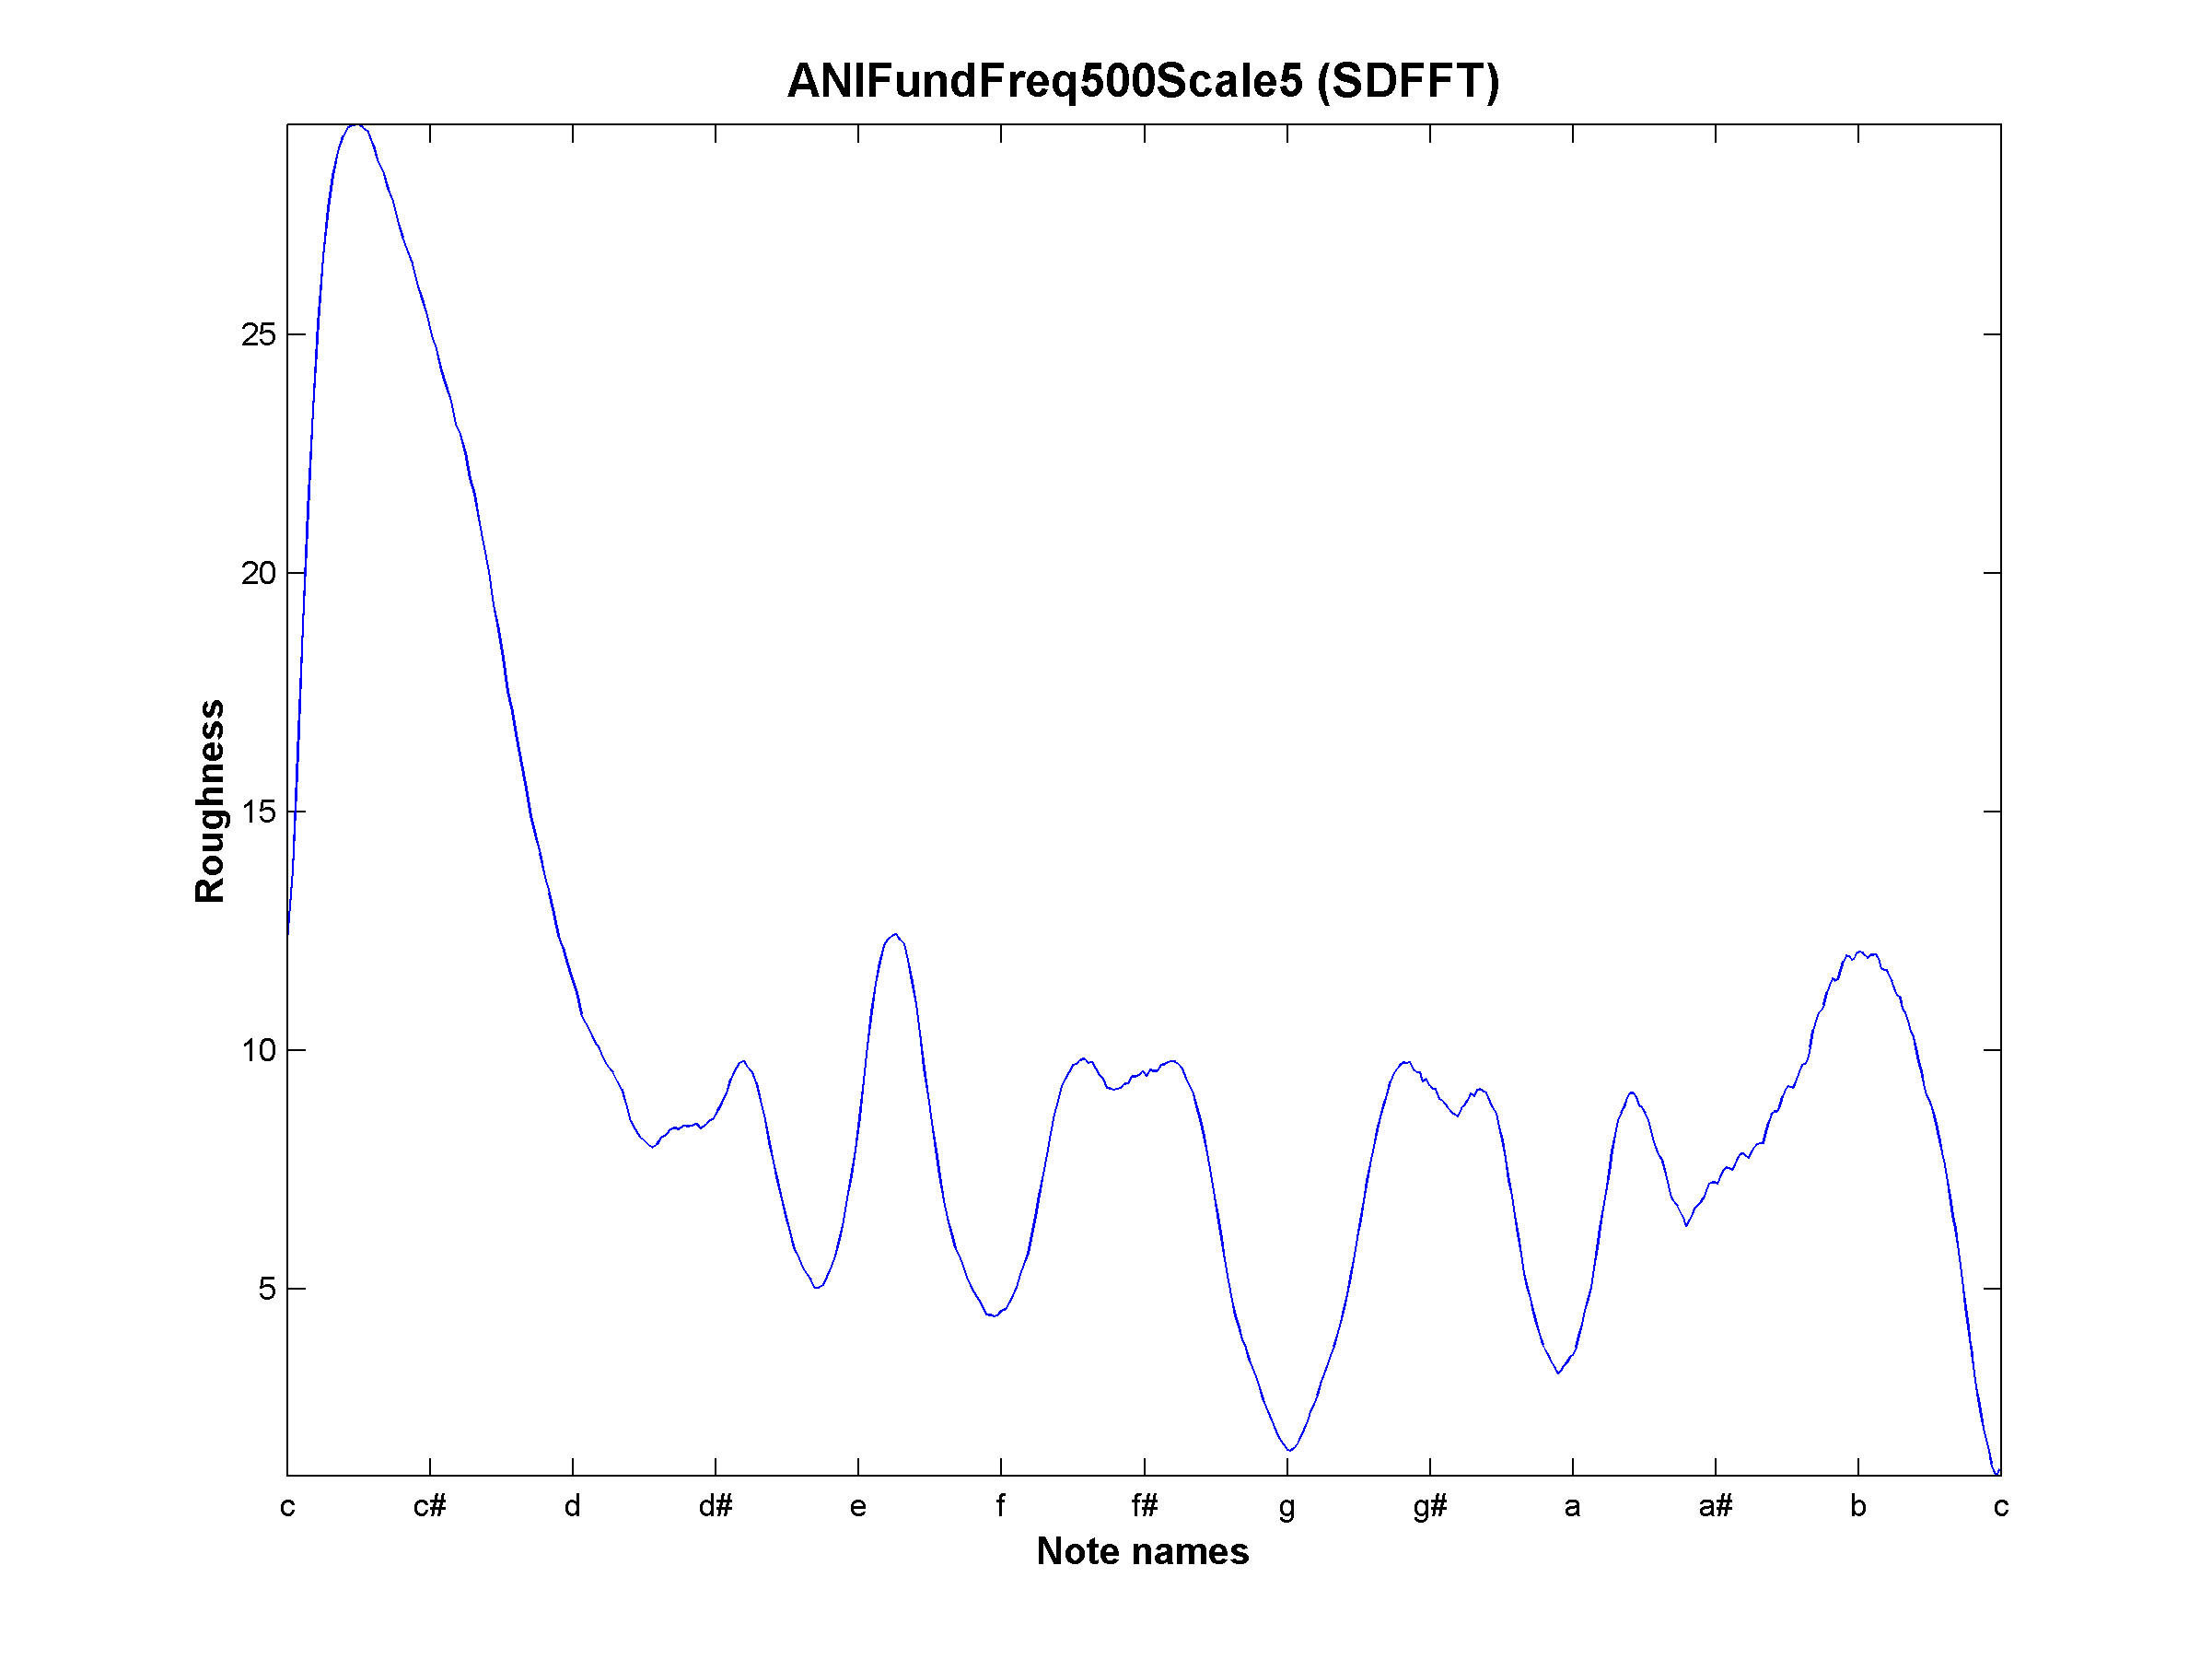
\includegraphics[width=\IPEMDefaultFigureWidth]{Graphics/RoughnessExperiments33}
    \caption{Roughness as calculated with the Synchronization Index Model}
    \label{Fig:RoughnessExperiments33}
\end{figure}

\subsection{Results and discussion}
% --------------------------------------------------------------------------------
\subsubsection*{Dependency}
% --------------------------------------------------------------------------------
The dependency of roughness on $m$, $f_m$ and $f_c$ provides
evidence for the theory that roughness may be directly related to
the degree in which neurons synchronize with the beating
frequencies of the AM tones. Roughness should then depend on two
basic effects:
\begin{itemize}
\item
The 'spectral' filtering resulting from the resonance properties
of the basilar membrane.
\item
The neuronal synchronization and its possible limitations.
\end{itemize}

\subsubsection*{Modulation frequency smaller than 25 Hz}
% --------------------------------------------------------------------------------
For $f_m$ smaller than about 25 Hz, the sensation of roughness
goes over into a sensation of fluctuation and loudness. Roughness
starts at about $f_m > 25 $ Hz but then the effects of spectral
filtering and synchronization should be taken into consideration.

\subsubsection*{Frequencies outside the filter bandwith}
% --------------------------------------------------------------------------------
AM tones have spectral energy at both sides ($f_c \pm f_m$) of a
carrier frequency $f_c$. An increase of the modulation frequency
$f_m$ results in a widening of the intervals. Consequently, when
the side frequencies ($f_c \pm f_m$) fall outside the central
scope of the $f_c$ filter bandwidth, their energy becomes more
and more attenuated and the beating decreases in relation to
that. The bandwidth of the auditory filters corresponds to
resonance regions of equal distance on the basilar membrane
\cite{GreenwoodJoris:1996}. Due to the quasi logarithmic
relationship between distance and frequency, the filter bandwidth
of this filter becomes broader in the higher frequency regions.
The 'spectral' filtering that results from the resonance
properties of the basilar membrane accounts for the fact that the
roughness decreases when $f_m$ exceeds the bandwidth of the
filtering associated with $f_c$. As the frequency components
exceed the bandwidth of an auditory filter, they will no longer
interfere and will cease to produce beating frequencies.

\subsubsection*{Frequency components within the filter bandwidth}
% --------------------------------------------------------------------------------
In the case, when the frequency components fall within the
bandwidth of the spectral filter, the neurons will attempt to
synchronize to the beating frequencies provided that those
frequencies are not too fast. Analysis of neuronal responses in
the auditory nerve indicates that neuronal synchronization has an
upper limit at about 1000 Hz which implies an absolute limit for
inferences based on synchronization \cite{JorisYin:1992}. But fast
beating frequencies, however, will be picked up as pitches rather
than roughness \cite{SchreinerLangnerNeuro:88a}. Only the beating
frequencies (e.g.~$25 Hz < f_m < 300$ Hz), will contribute to
roughness, suggesting that synchronization is actually subjected
to a band-pass filtering.

\subsubsection*{Conclusion}
% --------------------------------------------------------------------------------
The synchronization index model offers a standard method in the
calculation of the modulation depth for roughness. The method
allows a proper visualization of the features that contribute to
roughness both in terms of fluctuations in the auditory channels,
and in terms of phase-locking synchrony. The visualization
provides interesting cues for analyzing the factors that
contribute to roughness.

% --------------------------------------------------------------------------------

% --------------------------------------------------------------------------------
% --------------------------------------------------------------------------------
\newpage
\section{Tonality induction experiments}
% --------------------------------------------------------------------------------

% Make target for following functions:
\hypertarget{Concepts:IPEMGenerateProbes}{}
\hypertarget{Concepts:IPEMProbeToneExperimentKK1}{}
\hypertarget{Concepts:IPEMProbeToneExperimentKK2}{}

\subsection{Introduction}
% --------------------------------------------------------------------------------

In this demonstration contextuality is applied to simulate two
psychological experiments described by
\citeA{KrumhanslKessler:82}. The application is based on an
auditory model testing the role of short-term memory in probe-tone
experiments \citeA{Leman?}. The paper investigates the
relationship between short-term memory and the probe-tone
technique by means of auditory modeling. The results of the
simulation of the probe-tone Experiment I and Experiment II of
Krumhansl and Kessler show that a short-term memory model, based
on echoic images of periodicity pitch patterns, gives a good fit
with the probe-tone ratings.

\subsection{Method}
% --------------------------------------------------------------------------------

The probe-tone technique inspects a tonal context by means of
probe-tones. The listener hears a chord or a scale in order to
establish a key, then a probe tone is presented and the listener
is asked to rate how well that tone fits within the key being
examined. \citeA{KrumhanslKessler:82} take the technique as an
experimental paradigm for the study of context-dependent pitch
perception. The tonal context is generated by a so-called {\sl
context-defining sequence}, which is usually a harmonic
progression of chords expressing a stable major or minor key, but
a major or minor scale of pitches can be used as well. After
presentation of the context-defining sequence followed by a probe,
the listener is asked to rate the degree of fit between probe and
sequence on a scale. The probe is varied over all 12 pitches of
the chromatic scale hence 12 trials are needed to probe a
context-defining sequence. The responses obtained for those 12
trials specify a (tonal hierarchy) {\sl profile}.\\ The
simulations are done using an auditory pitch model. They aim to
process the stimuli given to human subjects in the psychological
experiments. The simulated probe-tone ratings are focussed on
stimulus-driven inferences. The
\hyperlink{Concepts:ContextualityModule}{Contextuality Module} is
aimed at simulating the degree-of-fit task of probe-tone
experiments. Simulation I and II cover all essential steps in the
probe-tone experiments of Krumhansl and Kessler.

\subsubsection*{Framework}
% --------------------------------------------------------------------------------
The auditory workspace for the simulation of the probe-tone
experiments draws on the distinction between
\hyperlink{Part:ConceptsIntroduction}{\emph{auditory images,
processes and inferences}}. The modules involved in the auditory
model are the
\hyperlink{Concepts:AuditoryPeripheralModule}{Auditory Peripheral
Module}, the \hyperlink{Concepts:PitchCompletionModule}{Pitch
Completion Module}, the
\hyperlink{Concepts:EchoicMemoryModule}{Echoic Memory Module} and
the \hyperlink{Concepts:ContextualityModule}{Contextuality
Module}. An auditory peripheral system transforms sound waveforms
into auditory patterns or primary images. The Pitch Completion
Module then transforms the primary images into pitch images. The
stimulus-driven inference is based on a comparison of images
having undergone the effect of an echo. To measure pitch
commonality between pitch images Leman uses two types of
stimulus-driven inference called Method I and Method II.
\begin{itemize}
\item Inspection:\\
    In the first method stimulus-driven inference has
    been interpreted as an inspection of the profile build-up during
    the temporal deployment of the context-defining sequence. A local
    image is fixed at the end of the probe-tone. Running images over
    the whole stimulus are inspected by means of this image.
\item Comparison:\\
    In the second method pitch images with possible
    different echo are compared at running time. Method II assumes
    two memory buffers whose size corresponds to the size of a local
    plus a global image. Both buffers are updated at run time and
    operate as echoic memories.
\end{itemize}

\subsection{Application}
% --------------------------------------------------------------------------------

\subsubsection*{Simulation of probe-tone experiments}
% --------------------------------------------------------------------------------
The short-term memory models related to the methods of inspection
and comparison for measuring the pitch commonality of local versus
global pitch images are used in Simulation I and II of Krumhansl
and Kessler's Experiment I and II \cite{KrumhanslKessler:82}.

\subsubsection*{Performance}
% --------------------------------------------------------------------------------
The contents of the demonstration package for the contextuality
experiments can be found in the directory
IPEM$\backslash$Demos$\backslash$Contextuality. To perform the
simulation of Experiment I and II described by Krumhansl and
Kessler first create the periodicity pitch patterns of all
pitches and chords used in order to construct the sounds. The
calculations are done using the function
\hyperlink{FuncRef:IPEMGenerateProbes}{IPEMGenerateProbes}. The
periodicity pitch results and the signals for the sound sequences
are stored in the directory PitchImagesShepardTone, relative to
IPEMRootDir ('output')$\backslash$ContextualityDemo. The content
of this directory takes 8,44Mb. Then perform the two simulations
with the functions
\hyperlink{FuncRef:IPEMProbeToneExperimentKK1}{IPEMProbeToneExperimentKK1}
and
\hyperlink{FuncRef:IPEMProbeToneExperimentKK2}{IPEMProbeToneExperimentKK2}.\\\\

\underline {Remark:} Note that performing this demonstration is
time-consuming for it takes around 2 hours and 30 minutes on a
Windows NT 4.0 system with Pentium III 600 MHz processor, 256Mb
RAM PC130.

\subsubsection*{Simulation I}
% --------------------------------------------------------------------------------
Simulation I corresponds to Experiment I that probed for the
major and minor key templates. In Experiment I, Krumhansl and
Kessler used twelve different context-defining elements, called
here {\sl sequences}. (In our terminology, a sequence may have
one single tonal element.) The sequences are shown in Table
\ref{table_one}.
%
\begin{table}[!h]
\footnotesize
\begin{tabular}{lll}

&Context-Defining Element& Example \\ \hline 1. &Ascending major
scale & $c~d ~e~ f~ g ~a ~b ~c$ \\ 2. &Ascending harmonic minor
scale & $c~ d~ e\flat~ f~ g~ a\flat~ b~ c$ \\ 3. &Major chord &
$c~ e~ g$ \\ 4. &Minor chord & $c~ e\flat~ g$ \\ 5. &Diminished
chord & $c~ e\flat~ g\flat$ \\ 6. &Dominant seventh chord & $c~ e~
g~ b\flat$ \\ 7. &IV-V-I cadence in major & $F~ maj~ chord~~ G~
maj~ chord~~ C~ maj~ chord $ \\ 8. &II-V-I cadence in major & $D~
min~ chord~~ G ~maj~ chord ~~C ~maj ~chord $ \\ 9. &VI-V-I cadence
in major & $A ~min~ chord~~ G~ maj ~chord~~ C ~maj ~chord $ \\ 10.
&IV-V-I cadence in minor & $F~ min~ chord~~ G ~maj ~chord ~~C~ min
~chord $ \\ 11. &II-V-I cadence in minor & $D~ dim ~chord ~~G
~maj~ chord ~~C ~min~ chord $ \\ 12. &VI-V-I cadence in minor &
$A\flat~ maj ~chord ~~G ~maj ~chord ~~C~ min ~chord $ \\

\end{tabular}
\caption{Context Defining Elements Used in Experiment 1}
\label{table_one}
\end{table}\\

Each trial consists of a context-defining sequence followed by a
probe tone. Given 12 sequences and 12 probes, this gives 12 x 12 =
144 trials. On each trial, the context-defining sequence was heard
first, followed by a one-second pause, and then the probe sounded
for 0.5 seconds. The timings of the different context-defining
sequences were as follows: the tonic tones of the two scales
(major and minor) were sounded for 0.5 seconds, and the remaining
scale tones for 0.25 seconds, with a 0.19-seconds pause between
scale tones. The single-chord sequences were played for 0.5
seconds, as were the chords in the three-chord cadences. In the
cadences there was about 0.25 seconds between chords. In order to
achieve stylistic neutrality, the tones used in all trials were
Shepard tones.

Simulation I uses the same 144 trials. First the sounds are
processed with \hyperlink{Concepts:AuditoryPeripheralModule}{APM},
\hyperlink{Concepts:PitchCompletionModule}{PCM}, and
\hyperlink{Concepts:EchoicMemoryModule}{EMM}, into local and
global images. The echos are respectively set to $T=0.1$ and
$T=1.5$. The stimulus-driven inference is calculated for each
trial and a snapshot is taken at the end of the trial. (Method I
and Method II deliver the same results at this point.) The
snapshots of all 12 different probe tones for one single
context-defining sequence then represents the profile of that
sequence. At the end, there are 12 profiles, corresponding to the
12 context-defining sequences of Table \ref{table_one}. Figure
\ref{Fig:TonalityDemoFig8} shows the twelve profiles that result from this
simulation. The number to the left of each graph corresponds with
the number of the context-defining sequence in Table
\ref{table_one}.

\begin{figure}[h]
    \centering
    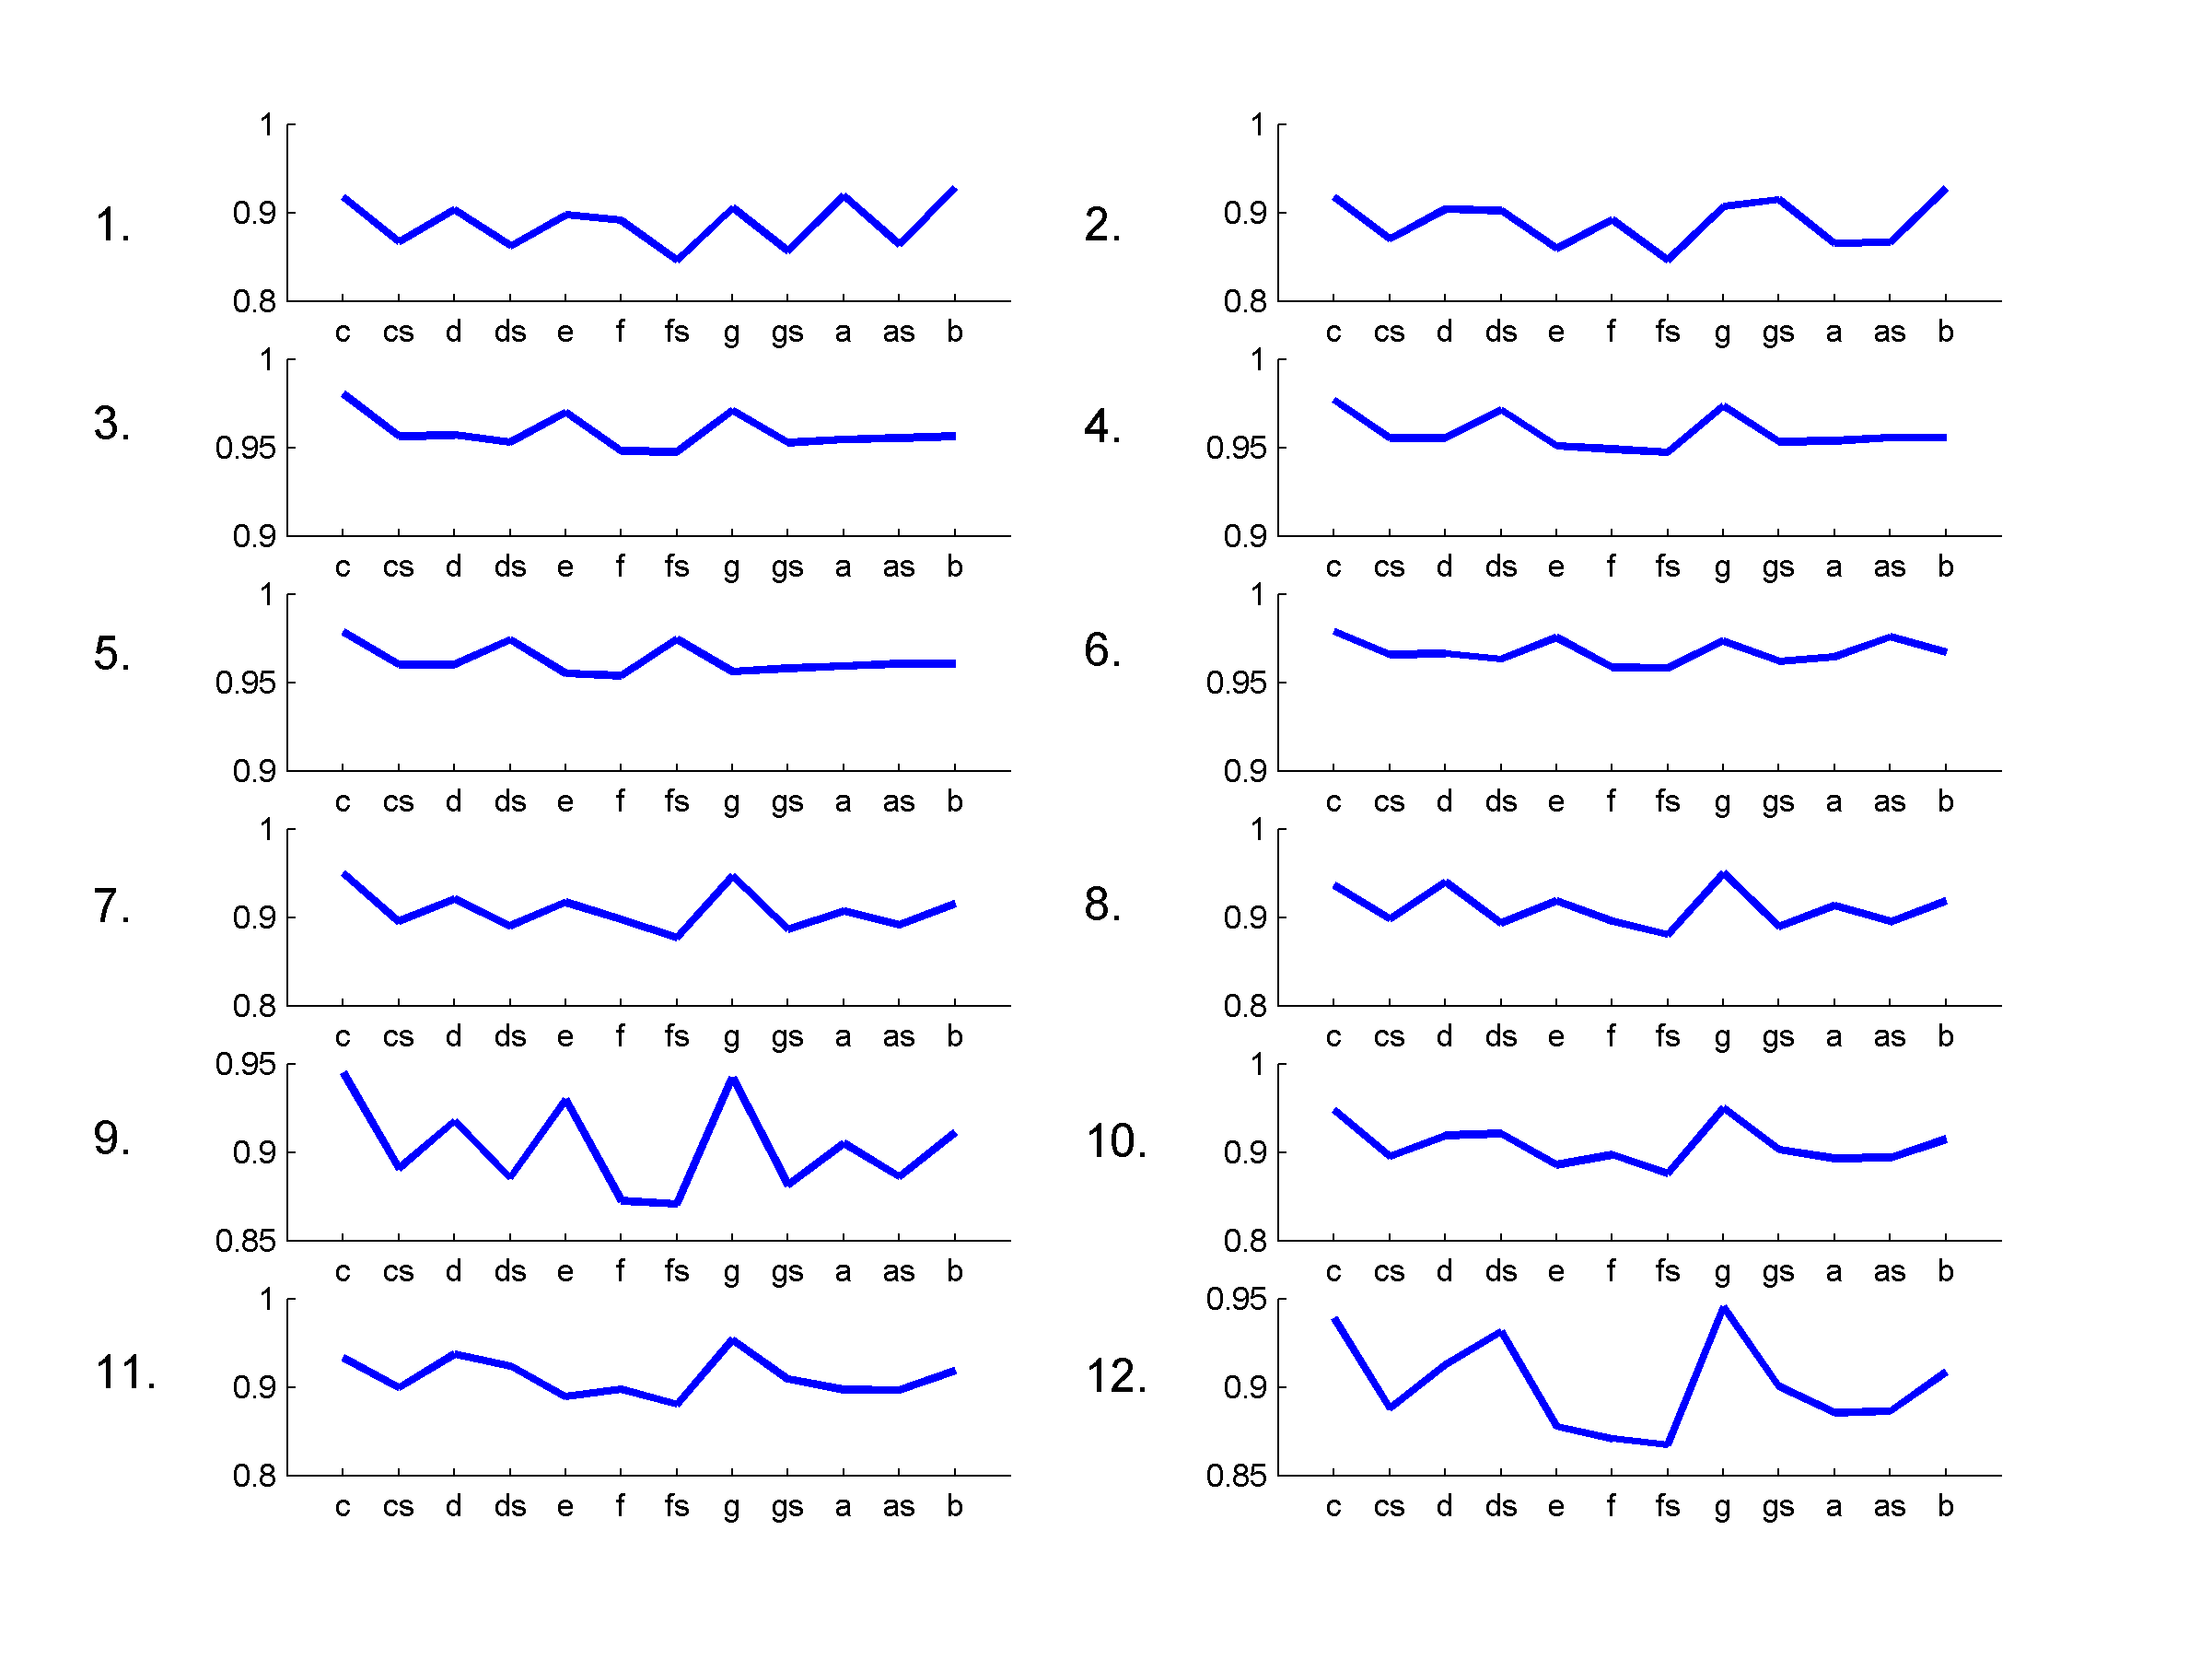
\includegraphics[width=\IPEMDefaultFigureWidth]{Graphics/TonalityDemoFig8}
    \caption{Profiles of 12 context-defining sequences for tone center $T=1.5$.}
    \label{Fig:TonalityDemoFig8}
\end{figure}

For each figure, the vertical axis represents the correlation
between the local image and the global image at the end of the
trial (12 trials are represented in each figure). What matters is
the relative relationships between the correlation coefficients
within a profile. In fact, when profiles are compared with each
other, using the correlation coefficient as a measure of
comparison, then the relative values are important. Table
\ref{table_two} shows the similarities among the twelve profiles.

\begin{table}[!h]
\footnotesize
\begin{tabular}{l|llllllllllll}
element&1.&2.&3.&4.&5.&6.&7.&8.&9.&10.&11.&12 \\ \hline 1.
&1.000&0.457&0.421&0.219&-0.226&0.336&0.709&0.720&0.665&0.428&0.408&0.315\\
2.
&&1.000&0.208&0.439&-0.024&0.090&0.404&0.384&0.289&0.698&0.708&0.671\\
3.
&&&1.000&0.670&0.163&0.867&0.865&0.724&0.916&0.647&0.492&0.589\\
4. &&&&1.000&0.466&0.531&0.647&0.525&0.588&0.887&0.756&0.923\\ 5.
&&&&&1.000&0.053&0.000&-0.140&0.010&0.224&0.065&0.332\\ 6.
&&&&&&1.000&0.677&0.577&0.770&0.457&0.334&0.435\\ 7.
&&&&&&&1.000&0.938&0.940&0.794&0.712&0.659\\ 8.
&&&&&&&&1.000&0.910&0.727&0.768&0.629\\ 9.
&&&&&&&&&1.000&0.662&0.609&0.611\\ 10.
&&&&&&&&&&1.000&0.936&0.943\\ 11. &&&&&&&&&&&1.000&0.917\\ 12.
&&&&&&&&&&&&1.000\\
\end{tabular}
\caption{The correlation coefficients represent the similarity
between the profiles, for the 12 context-defining sequences used
in Simulation I}
\label{table_two}
\end{table}
%
The following observations can be made:
\begin{itemize}
\item
Sequence 1 (major scale) correlates best with sequences 7, 8, and
9 (the cadences in major). The average correlation between the
major scale (1) and the three cadences in major (7, 8, 9) is
0.698. It was 0.796 in the data of Krumhansl and Kessler.
\item
Sequence 2 (minor scale) correlates best with sequences 10, 11, 12
(the cadences in minor). The average correlation between the minor
scale (2) and the three cadences in minor (10, 11, 12) is 0.6923.
It was 0.727 in the data of Krumhansl and Kessler
\item
Sequence 3 (major chord) correlates best with sequences 6, 7, 8,
and 9 (dominant seventh chord and major cadences). The average
correlation between the major chord (3) and the three cadences in
major (7, 8, 9) is 0.835. It was 0.896 in the data of Krumhansl
and Kessler.
\item
Sequence 4 (minor chord) correlates best with sequences 10, 11, 12
(minor cadences). The average correlation between the minor chord
(4) and the three cadences in minor (10, 11, 12) is  0.855. It was
0.910 in the data of Krumhansl and Kessler.
\item
Sequence 5 (diminished chord) has a low correlation with all other
sequences.
\item
Sequence 6 (dominant seventh chord) has the highest correlation
with sequence 9 (VI V I cadence in major).
\item
All cadences in major are strongly connected, and all cadences in
minor are strongly connected.
\end{itemize}

Krumhansl and Kessler concluded that the major chord element and
the three cadences in major indicate a consistent pattern of
ratings. In a similar way, the major scale was somewhat less
similar. They therefore took the major key profile as the average
ratings, given the 12 probe tones, for the major chord and the
three cadences in major. In correspondence with this idea, and
justified by the results shown in Table \ref{table_two}, the major
key profile of Simulation I is defined as the average of the
profiles that correspond to the sequences 3, 7, 8, and 9. The
minor key profile of Simulation I is determined according to the
same reasoning, taking the average of the profiles that correspond
to the sequences 4, 10, 11, and 12. The similarity of the major
key profile of Experiment I with the major key profile of
Simulation I has correlation coefficient of 0.848. The similarity
of the minor key profile of Experiment I with the minor key
profile of Simulation I is 0.825. This is a significant
correlation showing that the short-term memory model gives a good
account of the data in Experiment I.\\ An important parameter of
the model pertains to the echo of the global images. In order to
clarify the role of the echo, a series of simulations are carried
out in which the echo of the global image is systematically
varied from $T=0.2$ to $T=5$ in steps of 0.2. Twenty-five figures
are plotted that show the effect of changing the echo $(T)$ of the
global images on the profiles of the 12 context-defining
sequences. Each time the 144 trials are processed. Figures
\ref{Fig:TonalityDemoKK1Fig2} to \ref{Fig:TonalityDemoKK1Fig17} show the 12 profiles for
halfdecay tone centers with the echo set to $T=0.4$, $T=1.4$, $T=2.4$ and $T=3.4$\\

\begin{figure}[p]
    \centering
    \includegraphics[width=\IPEMDefaultFigureWidth]{Graphics/TonalityDemoKK1Fig2}
    \caption{Profiles of 12 context-defining sequences for tone center $T=0.4.$}
    \label{Fig:TonalityDemoKK1Fig2}
\end{figure}

\begin{figure}[p]
    \centering
    \includegraphics[width=\IPEMDefaultFigureWidth]{Graphics/TonalityDemoKK1Fig7}
    \caption{Profiles of 12 context-defining sequences for tone center $T=1.4.$}
    \label{Fig:TonalityDemoKK1Fig7}
\end{figure}

\begin{figure}[p]
    \centering
    \includegraphics[width=\IPEMDefaultFigureWidth]{Graphics/TonalityDemoKK1Fig12}
    \caption{Profiles of 12 context-defining sequences for tone center $T=2.4.$}
    \label{Fig:TonalityDemoKK1Fig12}
\end{figure}

\begin{figure}[p]
    \centering
    \includegraphics[width=\IPEMDefaultFigureWidth]{Graphics/TonalityDemoKK1Fig17}
    \caption{Profiles of 12 context-defining sequences for tone center $T=3.4.$}
    \label{Fig:TonalityDemoKK1Fig17}
\end{figure}

\subsubsection* {Simulation II}
% --------------------------------------------------------------------------------

Simulation II corresponds to Experiment II that aimed at sensing
directly how the listener's sense of key develops and changes,
providing a quantitative measure of the relative strengths of
tonal interpretations at each point in time. The test uses 10
different chord sequences containing modulations from one key to
another key. Table \ref{ChordSequences} gives an overview of the
10 different chord sequences. The sequences, ordered from 1 to 10
are each composed of 9 chords. They have a starting key and an
ending key, and the modulation from one key to the other key can
be direct, indirect, close, or remote.\\
Sequence 1 has no modulation, starting and ending key are in C
major.\\
Sequence 2 has no modulation, starting and ending key are in C
minor.\\
Sequence 3 has a direct and close modulation, starting in C major
and ending in G major.\\
Sequence 4 has an indirect and remote modulation, starting in C
major and ending in B$\flat$ major.\\
Sequence 5 has a direct and close modulation, starting in C major
and ending in A minor.\\
Sequence 6 has an indirect and remote modulation, starting in C
major and ending in D minor.\\
Sequence 7 has a close modulation, starting in C minor and ending
in F minor.\\
Sequence 8 has a remote modulation, starting in C minor and
ending in C$\sharp$ minor.\\
Sequence 9 has a close modulation, starting in C minor and ending
in C major.\\
Sequence 10 has an indirect and close modulation, starting in C
minor and ending in A$\flat$ major.\\
\begin{table} [!h]
    \footnotesize
    \centering
    \small Chords\\ \vspace{1cm}
    \begin{tabular}{l|lllllllll}
        % after \\ : \hline or \cline{col1-col2} \cline{col3-col4} ...
        & 1 & 2 & 3 &4 & 5 & 6 & 7 & 8 & 9 \\ \\\hline\\
        Seq.~1: & Fmaj & Gmaj & Amin        & Fmaj & Cmaj & Amin  & Dmin   & Gmaj &
        Cmaj\\\\
        Seq.~2: & Fmin & Gmaj & A$\flat$maj & Fmin & Cmin & A$\flat$maj & Ddim & Gmaj & Cmin \\\\
        Seq.~3: & Fmaj & Gmaj & Cmaj & Amin & Emin & Bmin & Emin & Dmaj & Gmaj \\\\
        Seq.~4: & Fmaj & Gmaj & Cmaj & Amin & Fmaj & Gmin & E$\flat$maj & Fmaj & B$\flat$maj \\\\
        Seq.~5: & Fmaj & Gmaj & Cmaj & Fmaj & Dmin & Emaj & Bdim & Emaj & Amin \\\\
        Seq.~6: & Fmaj & Gmaj & Cmaj & Fmaj & Dmin & B$\flat$maj & Edim & Amaj & Dmin \\\\
        Seq.~7: & Ddim & Gmaj & Cmin & A$\flat$maj & Fmin & D$\flat$maj & B$\flat$min &
        Cmaj & Fmin \\\\
        Seq.~8: & Ddim & Gmaj & Cmin & Gmaj & A$\flat$maj & Amaj & F$\sharp$min &
        G$\sharp$maj & C$\sharp$min \\\\
        Seq.~9: & Ddim & Gmaj & Cmin & A$\flat$maj & Gmaj & Amin & Fmaj & Gmaj & Cmaj \\\\
        Seq.~10: & Ddim & Gmaj & Cmin & A$\flat$maj & Fmin & E$\flat$maj & B$\flat$min &
        E$\flat$maj & A$\flat$maj \\\\
    \end{tabular}
    \caption{\ Chord Sequences Used in Experiment II.
    Cmaj means the C major chord, Cmin the C minor chord, and Cdim,
    the C diminished chord.}
    \label{ChordSequences}
\end{table}

A single chord sequence consists of 9 chords and for each
sequence, there were 9 trials. In the first trial, the
context-defining sequence was limited to the first chord and the
listeners were asked to probe the chord with the 12 probe tones.
In the second trial, the context-defining sequence was made of the
first two chords of the sequence and the listeners were asked to
probe this two-chord sequence with the 12 probe tones. In the
third trial, the context-defining sequence was made of the first
three chords of the sequence and the listeners were asked to probe
the sequence with the 12 probe tones, and so on. In the ninth
trial, the context-defining sequence was equal to the complete
sequence. For each chord sequence, one thus obtained 9 profiles
containing information about the gradual temporal deployment of
the tonal sequence. The 10 different chord sequences thus
correspond to 10 different {\sl profile-sequences}, each
containing 9 profiles.\\\\

The analysis of a profile-sequence had two parts. In the first
part the analysis was done in reference to the profile of the
first key of the corresponding chord sequence. In the second part,
the analysis was done in reference to the second key of the
corresponding chord sequence. Thus, if the chord sequence started
in C major, and modulated to G major, then the first analysis
correlated each profile of the sequence with the profile of the C
major key. The second analysis correlated each profile of the
sequence with the profile of the G major key. One thus obtained
for each chord sequence two (nine-step) {\sl
correlation-sequences}, one correlation-sequence representing the
sense of key with respect to the first key, another
correlation-sequence representing the sense of key with respect to
the second key.\\\\

Simulation II has then been set up as follows. The 10 chord
sequences with 9 subsequences each, define 90 context-defining
sequences. Each sequence was processed as follows:
\begin{enumerate}
\item
    The sound $s(t)$ of the chord sequence is processed with the
    auditory model (APM, PCM, and EMM) into local and global images.
    The echos are set to $T=0.1$ and $T=1.5$.
\item
    The global images $\tilde{p}_{T=1.5}(t)$ are inspected by the 12
    different probes tones using the stimulus-driven inference Method
    I. This was done in order to get an insight into the way in which
    the profile-sequence is built up at run-time. Figure
    \ref{Fig:TonalityDemoFig11} shows the profile-sequence for the global images
    inspected by the probe tones. Chord sequence 4 is used as an
    example.
\item
    In a similar way, the local images $\tilde{p}_{0.1}(t)$ are
    inspected by the 12 different probes tones using the
    stimulus-driven inference Method I. Figure \ref{Fig:TonalityDemoFig12} shows
    the profile-sequence of chord sequence 4 for the local images
    inspected by the probe tones.
\item
    The profiles are then correlated with the major and minor key
    profiles of Simulation I, in agreement to the setup of Experiment
    II. The key profiles are obtained by rotation of the C major and C
    minor key profiles of Simulation I, similar to the approach taken
    by Krumhansl and Kessler.
\item
    Finally, the averaged correlations are taken according to the
    series specified in the original simulation, that is: (i) average
    chord sequences 1 and 2, (ii) average chord sequences 3, 5, 7, 9,
    10 for the first key, and for the second key, (iii) average chord
    sequences 4, 6, and 8 for the first key, and for the second key.
\end{enumerate}

\begin{figure}[h]
    \centering
    \includegraphics[width=\IPEMDefaultFigureWidth]{Graphics/TonalityDemoFig11}
    \caption {Stimulus-driven inferences (Method I) of chord sequence 4 used in Simulation II. The labels
    specify major and minor chords and are located at the time instances where they are
    introduced.
    The context-defining sequence is probed with 12 different probe tones. The stimulus-driven inference
    for each trial is plotted. The buildup and decay of the inferences depends on the echo of the global images
    ($T=1.5$). The dotted line represents the probe tone $c$, the solid line represents the probe tone $b\flat$}
    \label{Fig:TonalityDemoFig11}
\end{figure}

\begin{figure}[h]
    \centering
    \includegraphics[width=\IPEMDefaultFigureWidth]{Graphics/TonalityDemoFig12}
    \caption{Stimulus-driven inferences (Method I)of chord sequence 4 used in Simulation II.
     The global images have the same echo as the local images ($T=0.1$). The dotted line represents the probe tone f.}
    \label{Fig:TonalityDemoFig12}
\end{figure}

The effects of echo are clearly visible in
Fig.~\ref{Fig:TonalityDemoFig11}. At the beginning of the
sequence, one gets the same profile for the F major chord as in
Fig.~\ref{Fig:TonalityDemoFig12}. But the next chords, G major and
then C major lead to quite different profiles, owing to the effect
of the echo. The dotted line shows the correlation with the probe
tone $c$, the tonic of the first key, the full line shows the
correlation with the probe tone $b\flat$, the tonic of the second
key. Shuffling chords around may have an effect on the resulting
profile. Certain chord progressions will prevent certain pitches
to pop up, while other chord progressions will favor other pitches
in the profile. But the echo takes into account the temporal order
of the chords, provided that it is within the limits of the half
decay time.

\subsection{Results and discussion}
% --------------------------------------------------------------------------------
Using the same stimuli as in Experiment I and Experiment II of
Krumhansl and Kessler \cite{KrumhanslKessler:82}, the short-term
memory model produces a good fit with the data. A comparison of
the key profiles of Simulation I with those obtained in Krumhansl
and Kessler's Experiment I gives a correlation of 0.848 for the
major key, and 0.825 for the minor key. The echo, or half decay
time, of the global image, which determines the content of the
context-defining sequence, was determined to be about 1.5 seconds.
Using this echo, Simulation II aimed at repeating Krumhansl and
Kessler's Experiment II in which the dynamic aspects of key
sensitivity were investigated.

\subsubsection*{Simulation I}
The results of Simulation I are summarized in Table
\ref{table_three}.
\begin{table}[!h]
\footnotesize
\begin{tabular}{lllllll}
T (=echo) & 1 vs 7+8+9 & 2 vs 10+11+12& 3 vs 7+8+9 & 4. vs
10+11+12 & KKMajor & KKMinor\\ \hline 0.2 & 0.989
&0.987&1.000&1.000&-0.519&-0.087 \\ 0.4 & 0.454& 0.531& 0.895&
0.891& 0.264& 0.493 \\ 0.6 & 0.258& 0.309& 0.907& 0.917& 0.771&
0.808 \\ 0.8& 0.390& 0.408& 0.891& 0.909& 0.809& 0.812 \\ 1
&0.509& 0.514& 0.872& 0.891& 0.827& 0.817 \\
1.2&0.603&0.601&0.855& 0.875& 0.838& 0.821 \\ 1.4& 0.672& 0.667&
0.841& 0.861& 0.845& 0.824 \\ 1.6&0.720& 0.714& 0.829& 0.850&
0.851& 0.826 \\ 1.8&0.755& 0.748& 0.820& 0.840& 0.855& 0.828 \\
2&0.780& 0.772& 0.813& 0.832& 0.858& 0.829 \\ 2.2&0.799& 0.790&
0.806& 0.826& 0.860& 0.830 \\ 2.4&0.813& 0.803& 0.801& 0.820&
0.863& 0.831 \\ 2.6 &0.824& 0.814& 0.796& 0.815& 0.864& 0.831 \\
2.8&0.831& 0.821& 0.792& 0.811& 0.866& 0.832 \\ 3&0.838& 0.827&
0.789& 0.807& 0.867& 0.832 \\ 3.2&0.843& 0.832& 0.786& 0.804&
0.868& 0.833 \\ 3.4&0.847& 0.836& 0.783& 0.801& 0.869& 0.833 \\
3.6&0.851& 0.839& 0.780& 0.798& 0.870& 0.833 \\ 3.8&0.853& 0.842&
0.778& 0.796& 0.870& 0.834 \\ 4&0.856& 0.844& 0.776& 0.794& 0.871&
0.834 \\ 4.2&0.858& 0.846& 0.775 &0.792& 0.871& 0.834 \\
4.4&0.860& 0.847& 0.773& 0.790& 0.872& 0.834 \\ 4.6&0.861& 0.849&
0.771& 0.788& 0.872& 0.834 \\ 4.8&0.862& 0.850& 0.770& 0.787&
0.873& 0.835 \\ 5&0.863&0.851&0.768&0.786&0.873&0.835 \\
\end{tabular}
\caption{The effect of changing the echo ($T$) of the global
images on profiles} \label{table_three}
\end{table}

The left column contains the half decay time $T$ of the global
images (the local images have a constant echo of $T=0.1$), the
first column reports the averaged correlation of the profile of
sequence 1 with the profile of sequences 7, 8, and 9. The second
column contains the average correlations of the profiles of
sequence 2 with those of sequences 10, 11, and 12, the third
column of 3 with 7, 8, 9, and the fourth of 4 with 10, 11, 12. The
last two columns contain the correlations of the major and minor
key profiles of Experiment I with those of Simulation I.

At $T=0.2$ the effect of the tonal context can be neglected. Hence
one gets high correlations between the profiles, but very low
correlations with the key profiles.  At $T=0.4$ the effect of
context is growing, but the local effects are still dominating.
For $T > 0.4$ the effect of context becomes visible and three
general trends can be distinguished:
\begin{itemize}
\item
The scale becomes more similar to the cadences, both for major and
minor.
\item
The chords become less similar to the cadences, both for major and
minor.
\item
The key profiles become more similar.
\end{itemize}
The trend can be explained in terms of the increasing contribution
of the tonic of the scale when $T$ increases. Taking into account
the data of Krumhansl and Kessler, who observed a less good
correlation with the scales than with the chords, the optimal echo
for global images is taken to be $T=1.5$. The effect is shown in
Fig.~\ref{Fig:TonalityDemoFig9}, where $T=4$, all other parameters
being equal.
\begin{figure}[h]
    \centering
    \includegraphics[width=\IPEMDefaultFigureWidth]{Graphics/TonalityDemoFig9}
    \caption{Stimulus-driven inference of the ascending C-major diatonic,
     using an echo of T=4 for the global images.}
    \label{Fig:TonalityDemoFig9}
\end{figure}

\subsubsection*{Simulation II}
The results of Simulation II Method I are summarized in five
graphs shown in Fig.~\ref{Fig:TonalityDemoFig100}.\\

Method I gives a useful insight in how the profiles are build up
during the temporal deployment of the chord sequence but the
actual build up of the profile should not be taken into
consideration when data are compared with the probe tone ratings.
What actually matters in that case is the snapshot taken at the
end of each trial of the chord sequence. This can be obtained with
either Method I or Method II. Fig.~\ref{Fig:TonalityDemoFig100}
shows the results when the average correlations are taken at the
end of each chord, for the nine chords in the
sequence.\\

\begin{figure}[!h]
    \centering
    \includegraphics[width=\IPEMDefaultFigureWidth]{Graphics/TonalityDemoFig100}
    \caption{Results of Simulation II. The horizontal axis represents time in hundreds of seconds. The
    vertical axis is the correlation.The average correlations are
    taken at the end of each chord, for the nine chords in the
    sequences. The buildup effect of the local profiles now
    disappears.}
    \label{Fig:TonalityDemoFig100}
\end{figure}

\begin{figure}[]
    \centering
    \includegraphics[width=\IPEMDefaultFigureWidth]{Graphics/TonalityDemoFig101}
    \caption{Results of Simulation II. Same graphs as previous figure, but the points
    at the end of each chord have been selected}
    \label{Fig:TonalityDemoFig101}
\end{figure}

The data of Experiment II are summarized as follows:
\begin{itemize}
\item
    The full line in the top left figure represents the average
    correlation-sequence for chord sequences 1 and 2. These chord
    sequences have no modulation, hence, the correlation-sequence for
    the first key is identical to the correlation-sequence for the
    second key. The data therefore collapse to a single figure.
\item
    The full lines in both middle figures represent the average
    correlation-sequences for chord sequences 3, 5, 7, 9 and 10. These
    chord sequences have a modulation between closely related keys.
    Given the two different keys, the results are split up in two
    figures, one left and one right figure. The full line on the left
    figure contains the averaged correlation-sequence with the first
    key. The full line on the right figure contains the averaged
    correlation-sequence with the second key.
\item
    The full lines of the bottom figures represent the average
    correlation-sequences for the chord sequences 4, 6, and 8. These
    chord sequences have a modulation between distant keys. The full
    line on the left figure contains the averaged correlation-sequence
    with the first key. The full line on the right figure contains the
    averaged correlation-sequence with the second key.
\end{itemize}
The dashed line in each of the left-sided figures represents the
averaged correlation between the profile of the individual chords
and the profile of the first key, at each of the nine steps. The
dashed line in each of the right-sided figures represents the
averaged correlation between the profile of the individual chords
and the profile of the second key, at each of the nine steps. For
example, in the top left figure, the dashed line of the first
point is the average of two correlations, in particular the
correlation between the profile of the F major chord, and the C
major key profile, and the correlation between the profile of the
F minor chord and the C minor key profile. (The chord profiles and
the key profiles used to calculate the dashed line were all
obtained in Experiment I.) The correlations between the individual
chord profiles and the key profiles predict how strongly each
chord in isolation would be expected to be related to the intended
key of the sequence and, thus, serve as a baseline against which
the strength of the intended key can be compared. There is a
striking similarity with the results of Krumhansl and Kessler
Experiment II. The correlation ranges show a good agreement for
both lowest and highest values. There is a small difference in
the comparison of profiles to the first key (=left colomn
figures). The listeners seem to sense the key already after the
second chord, which is not the case in the simulation, where the
correlations corresponding to the global and local images are
almost similar for the first two chords of the sequence.

% --------------------------------------------------------------------------------


\newpage
% --------------------------------------------------------------------------------
% Concepts: Applications
% --------------------------------------------------------------------------------

% ================================================================================
\chapter{Applications}
\hypertarget{Chapter:ConceptsApplications}{}
% ================================================================================

% --------------------------------------------------------------------------------
\section{Introduction}
% --------------------------------------------------------------------------------

Whereas the previous chapters handled the basic modules and a
comparison of their results with psychoacoustic data, this chapter
focuses on some more elaborated applications where these modules
are used in practice. Each of the sections in this chapter
contains:
\begin{itemize}
\item a small introduction in which the purpose of the application is explained
\item a description of the method that is used
\item a summary of how to run the application in practice using
the toolbox and its functions
\item an overview of the obtained results and a discussion thereof
\end{itemize}
The applications are explained from a practical viewpoint, and
each time a link is made between the related concepts and the
practical tools (MATLAB functions) available in the toolbox.\\

The following applications are included:
\begin{itemize}
\item Roughness applications: relationships between timbre, scales and roughness.
\item A rhythmic pattern extraction demonstration for extracting
repetitive rhythm patterns from a sound fragment.
\end{itemize}
Each application can be seen as a demonstration of one (or more)
module(s) that were handled in the first chapter. You can of
course freely experiment with the modules yourself and build some
new applications from the basic functions. If you think that
you've come up with something interesting, we would love to hear
about it!

% --------------------------------------------------------------------------------
% --------------------------------------------------------------------------------
\newpage
\section{Roughness applications}
% --------------------------------------------------------------------------------

% Make target for following functions:
\hypertarget{Concepts:IPEMCalcRoughnessOverSubparts}{}
\hypertarget{Concepts:IPEMGeneratePitchShiftScript}{}

\IPEMTBC (ask Marc for latest version since Koen sent it for that paper)

% --------------------------------------------------------------------------------
\subsection{Introduction}
% --------------------------------------------------------------------------------

% --------------------------------------------------------------------------------
\subsection{Method}
% --------------------------------------------------------------------------------

% --------------------------------------------------------------------------------
\subsection{Application}
% --------------------------------------------------------------------------------

% --------------------------------------------------------------------------------
\subsection{Results and discussion}
% --------------------------------------------------------------------------------

% --------------------------------------------------------------------------------

% --------------------------------------------------------------------------------
% --------------------------------------------------------------------------------
\newpage
\section{Rhythmic pattern extraction}
% --------------------------------------------------------------------------------

% Make target for following functions:
\hypertarget{Concepts:IPEMDemoStartMEC}{}
\hypertarget{Concepts:IPEMDemoMECRhythmExtraction}{}

% --------------------------------------------------------------------------------
\subsection{Introduction}
% --------------------------------------------------------------------------------

In this demonstration, the MEC algorithm from the
\hyperlink{Concepts:RhythmModule}{Rhythm Module (RhM)} is used to
detect and extract rhythmic patterns from a sound fragment.\\
The extracted patterns are then used to synthesize sound using
modulated AM noise, which allows for an auditive comparison
between the original sound and the sound resynthesized from what
the Rhythm Module has extracted.

% --------------------------------------------------------------------------------
\subsection{Method}
% --------------------------------------------------------------------------------

For the extraction of rhythmic patterns, we are interested in
periods ranging from roughly 50 ms to 5 seconds.\\
The signal that will be analyzed is a root-mean-square (RMS)
signal calculated every 10 ms over a frame of 20 ms. We can
calculate the RMS:
\begin{itemize}
\item of the signals in the different channels of the output of
an auditory model (which yields a multi-channel RMS signal)
\item of the sound signal itself (which yields a 1-dimensional RMS signal)
\end{itemize}
This energy signal is then first analyzed using the MEC algorithm
and the most prominent periods occurring in the RMS signal is
detected by finding the minimum in the calculated difference
values. In the first case, this can be done by detecting a minimum
for each channel separately (yields best period for each channel)
or by summing the difference values from all channels first and then
picking the minimum from there (yields a single best period for all channels).\\
Once the best periods are known, the patterns corresponding to
that period can be extracted from the RMS signal.\\
Then, a specific moment in time is chosen, and the extracted
patterns at that moment are used for a resynthesis in order be
able to listen to what the MEC algorithm has found as rhythmic
pattern.\\
For more detailed information on the Rhythm Module itself, see
page \pageref{Concepts:RhythmModule}.\\

% --------------------------------------------------------------------------------
\subsection{Application}
% --------------------------------------------------------------------------------

The contents and the functions for this demo on rhythmic pattern
extraction using MEC can be found in the directory
IPEMToolbox$\backslash$Demos$\backslash$MECPatternExtraction.\\
The main functions are:
\begin{itemize}
\item \hyperlink{FuncRef:IPEMDemoMECRhythmExtraction}{IPEMDemoMECRhythmExtraction}\\
    This demo function starts an interactive session in which you can
    select a sound file, set some basic parameters, analyze the sound using
    MEC and then resynthesize using the analysis results.
\item \hyperlink{FuncRef:IPEMDemoStartMEC}{IPEMDemoStartMEC}\\
    This demo function starts an entire MEC analysis run in one go
    (without interaction). It allows to set more parameters and to save
    the analysis results to a file.
\end{itemize}
Both demo functions are based on the core functions related to the
\hyperlink{Concepts:RhythmModule}{Rhythm Module (RhM)}. You can
have a closer look to the Matlab code of the demo functions to get
to know how these core functions are used, or just check out the
functions in the \hyperlink{Part:ReferenceManual}{Reference
Manual}.


\subsubsection*{Interactive demo}

Figure \ref{Fig:IPEMDemoMECRhythmExtractionChart} shows the
execution flow of IPEMDemoMECRhythmExtraction.

\begin{figure}[!h]
    \centering
    \includegraphics[width=8cm]{Graphics/IPEMDemoMECRhythmExtractionChart}
    \caption{Execution flow of IPEMDemoMECRhythmExtraction}
    \label{Fig:IPEMDemoMECRhythmExtractionChart}
\end{figure}

\begin{enumerate}
\item
    First of all, the user has to select the sound file he/she
    wants to analyze.\\
    Three example sound files are located in the directory containing
    the demo:
    \begin{itemize}
    \item Example 1: \IPEMSound{Sounds/BartokScherzoSuiteOp14.wav}{BartokScherzoSuiteOp14.wav}\\
        This is a short fragment from the beginning of the second movement "Scherzo"\\
        from "Suite op. 14" by B\'{e}la Bart\'{o}k (piano).
    \item Example 2: \IPEMSound{Sounds/TomWaitsBigInJapan.wav}{TomWaitsBigInJapan.wav}\\
        This is an excerpt from "Big in Japan" taken from "Mule Variations" by Tom Waits
        (voice, bass, drums, electric guitar).
    \item Example 3: \IPEMSound{Sounds/PhotekTheLightening.wav}{PhotekTheLightening.wav}\\
        This is a short fragment from "The Lightening (Digital Remix)" by Photek
        (electronic, drum and bass).
    \end{itemize}

\item
    Next, a few choices have to be made for setting the analysis parameters:
    \begin{itemize}
    \item Period range\\
        Specify the range of periods for which periodicity should be
        checked. For rhythmic patterns reasonable values are from 0.050 to 5
        seconds. The bigger the range, the more periods will be checked, so
        the slower the analysis will be.
    \item Type of analysis\\
        Finding the "best periods" can be done in three ways:
        \begin{itemize}
        \item using the difference values calculated from the RMS of
        the sound signal itself: this yields a single "best period" at
        each moment in time
        \item using the summed difference values (over all channels) calculated from the RMS of
        the ANI: this yields a single "best period" for all channels
        together at each moment in time
        \item using the difference values calculated from the RMS of
        the ANI separately for each channel: this yields a "best period" for each channel at each moment in
        time
        \end{itemize}
    \item Speed-up factor\\
        Instead of calculating difference values for every sample in the RMS
        signal, you can specify a speed-up factor n (a positive
        integer) so that values are calculated only every n samples.
    \item Pattern integration\\
        After extracting the patterns using the found best period
        at a certain moment, the patterns can be integrated over
        time. This can be done to decrease the effect of small local
        variations.
    \end{itemize}

\item
    Then, the sound file is read and the RMS is calculated with
    \hyperlink{FuncRef:IPEMCalcRMS}{IPEMCalcRMS}, either on the
    auditory nerve image of the sound, or on the sound itself,
    depending on what was specified in the previous step. The
    auditory nerve image is calculated with
    \hyperlink{FuncRef:IPEMCalcANI}{IPEMCalcANI} using 10 bands
    with a bandwidth of 1.5 critical band units (cbu), starting
    at 3 cbu. This corresponds to center frequencies of 215 Hz to
    3266 Hz.

\item
    The MEC algorithm then starts analyzing the RMS signal
    (\hyperlink{FuncRef:IPEMMECAnalysis}{IPEMMECAnalysis}) by calculating difference values.

\item
    Then the most prominent period(s) at each moment in time are selected.
    A figure with the best period(s) over time is generated (for RMS
    of ANI, this is a multi-channel plot, for RMS of sound
    signal, this is a single-channel plot).

\item
    The results of the previous analysis (the best period(s) at each
    moment) is then used to extract the corresponding pattern(s) from
    the RMS signal with
    \hyperlink{FuncRef:IPEMMECExtractPatterns}{IPEMMECExtractPatterns}.\\
    Depending on the specified parameters, these patterns can be
    further integrated over time with
    \hyperlink{FuncRef:IPEMLeakyIntegration}{IPEMLeakyIntegration}.

\item
    Finally, resynthesis of the extracted patterns can be done
    using \hyperlink{FuncRef:IPEMMECReSynthUI}{IPEMMECReSynthUI} (which
    calls
    \hyperlink{FuncRef:IPEMMECSynthesis}{IPEMMECSynthesis}
    internally.\\
    The presented user interface consists of two figures: one is
    the figure showing the (multi-channel) best periods over time
    and the other is a "control palette" with some push buttons.\\
    In the first figure, a moment in time (and a specific
    channel) can be selected by pressing the left mouse button.\\
    Once this selection is made, a resynthesis can be done by
    pressing the "Resynthesize for selected time" button. This
    button is only enabled when the selected time is different
    from the time for which resynthesis was last done.\\
    In order to evaluate the resynthesized sound, it is combined
    with the original sound into a stereo sound file, where the
    left channel plays the original sound and the right channel
    plays the synthesized sound. By pressing the "Play all
    channels" button, the last resynthesized sounds for all
    channels are played together, while the "Play selected
    channel" only plays the selected channel.\\
    Pressing a key (rather than clicking with the mouse) in the
    first figure ends the resynthesis.\\
    Figure \ref{Fig:MECDemoUI} shows a snapshot of the
    resynthesis user interface.

\end{enumerate}

\begin{figure}
    \centering
    \includegraphics[width=\IPEMDefaultFigureWidth]{Graphics/MECDemoPhotekTheLighteningUI}
    \caption{Resynthesis user interface}
    \label{Fig:MECDemoUI}
\end{figure}

\subsubsection*{One run demo function}

This demo function does essentially the same as the above
interactive demo, but it runs without any user intervention. All
parameters have to be specified when calling the function, and
then everything is calculated in one go, without interruption.

Figure \ref{Fig:IPEMDemoStartMEC} shows the execution flow of
IPEMDemoStartMEC.

\begin{figure}[h]
    \centering
    \includegraphics[width=\IPEMDefaultFigureWidth]{Graphics/IPEMDemoStartMEC}
    \caption{Execution flow of IPEMDemoStartMEC}
    \label{Fig:IPEMDemoStartMEC}
\end{figure}

The results of the analysis can be saved to a .mat file so that
resynthesis can be performed at a time later using either
\hyperlink{FuncRef:IPEMMECSynthesis}{IPEMMECSynthesis} or
\hyperlink{FuncRef:IPEMMECReSynthUI}{IPEMMECReSynthUI} after
reloading the data.


\subsubsection*{Remarks about the method of "resynthesis"}

The resynthesis is done by amplitude modulation of specific noise
bands with the extracted patterns. In case the RMS was calculated
on the auditory nerve image, the noise bands have a center
frequency equal to the center frequency of the corresponding
auditory channel. In case the RMS was calculated directly on the
sound signal, broad band noise is used. The resynthesized sound
pattern is then repeated until the total sound duration matches
that of the original sound.\\
Both are finally combined into a stereo sound where one channel
plays the original sound and the other plays the resynthesized sound.\\

Note that this "resynthesis" is just a "quick and dirty" way to
quickly hear the results of the pattern extraction. It assumes
that the entire sound is a constant repetition of the selected
pattern and this has a few important limitations:
\begin{enumerate}
\item drift\\
When the pattern is selected for the specified moment in time, it
is inserted before and after that moment as many times as needed
to obtain the total duration of the original sound. This means
that if there are small tempo fluctuations, the sound will only
match very well in the neighborhood of the selected moment in
time, but maybe not elsewhere. You might hear this "drifting" when
playing back the stereo sound.
\item gaps\\
This is a more extreme case of the above: when there is a gap in
the rhythmic flow (even if the tempo is constant), the
resynthesized sound will be out of sync with the original sound.
Again, only at the selected moment in time, there will be perfect
synchronization.
\item separated channels\\
When "separated channels" are used, a best period is found for
each channel, so it is perfectly possible that in the higher
channels a period was detected different from the one in the lower
channels. The resynthesis uses these patterns and you might thus
hear different patterns at the same time (each in a different
frequency range). This might be good for drum sequences where you
have different patterns for hihats and bass drum. If the pattern
lengths only differ slightly, again drift might be hearable.
\end{enumerate}


% --------------------------------------------------------------------------------
\subsection{Results and discussion}
% --------------------------------------------------------------------------------

\subsubsection*{Sound example 1}

Figure \ref{Fig:MECBartokExample} shows graphic results for the
sound example
\IPEMSound{Sounds/BartokScherzoSuiteOp14.wav}{BartokScherzoSuiteOp14.wav}.\\

The \emph{top left graph} shows the original sound and the
calculated RMS signal levels. It is this RMS signal that is
examined by the MEC analysis for repeating patterns.\\

The \emph{top right graph} shows the difference values calculated
by the MEC analysis together with the best period (corresponding
to the period for which the difference value is minimal).\\

The \emph{lower left graph} shows the effect of pattern
integration. A leaky integration with half decay time 0.5 s was
used, which has the effect that small differences between
successive patterns are eliminated in favor of a more stable
pattern. Of course, this also "flattens" the detected patterns and
"smears" them over time, so an appropriate choice for the half
decay time should be chosen.\\

The \emph{lower right graph} shows the graphical interface that
can be used for resynthesizing the rhythm starting from the
extracted patterns at a selected moment in time. To hear the
result of this "rhythm resynthesis" for this example, you can
listen to the following sound:
\begin{itemize}
\item[] - \IPEMSound{Sounds/MECDemoBartokScherzoSuiteOp14ReSynthAll.wav}{Resynthesis from RMS of sound}
\end{itemize}
This sound was resynthesized using repetitions of the pattern
extracted at 4.5 s, where a best period of 1.604 s was detected.
The left channel plays the original sound, while the right channel
plays the synthesized sound. The patterns in each channel were
rescaled between 0 and 1 (this is a parameter
of \hyperlink{FuncRef:IPEMMECExtractPatterns}{IPEMMECExtractPatterns}).\\

The signals of the synthesized sounds were further processed using
a third power function to enhance contrast in the sounds
($s_{enh}(t) = s(t)^3$, where $s(t)$ was first normalized between
-1 and 1). This is a parameter of the base function for
resynthesis of MEC results \hyperlink{FuncRef:IPEMMECSynthesis}{IPEMMECSynthesis}.\\


\subsubsection*{Sound example 2}

Figure \ref{Fig:MECTomWaitsExample} shows graphic results for the
sound example \IPEMSound{Sounds/TomWaitsBigInJapan.wav}{TomWaitsBigInJapan.wav}.\\

The \emph{top left graph} shows the auditory nerve image (ANI)
calculated for 10 bands having a configuration as explained in the interactive demo.\\

The RMS signal of this ANI is shown in the \emph{top right graph}.
It is this signal that is examined by the MEC analysis for repeating patterns.\\

The \emph{middle left graph} then shows the difference values
calculated by the MEC analysis together with the best period
(corresponding to the period for which the difference value is
minimal). Difference values were calculated for each channel and
then summed together to result in the shown overall difference
values.\\

The \emph{middle right graph} shows the effect of  pattern
integration. Again, a leaky integration with half decay time 0.5 s
was used.\\

The \emph{lower left graph} again shows the graphical interface
that can be used for resynthesizing the rhythm starting from the
extracted patterns at a selected moment in time. This resynthesis
can be done for each channel separately, but they all use the same
"best period" . To hear some examples of resynthesis, you can
listen to the following sounds:
\begin{itemize}
\item[] - \IPEMSound{Sounds/MECDemoTomWaitsBigInJapanReSynthANIAll.wav}{Resynthesis for all channels}
\item[] - \IPEMSound{Sounds/MECDemoTomWaitsBigInJapanReSynthANICh2.wav}{Resynthesis for channel 2}
\item[] - \IPEMSound{Sounds/MECDemoTomWaitsBigInJapanReSynthANICh9.wav}{Resynthesis for channel 9}
\end{itemize}
The sounds were in this case resynthesized using repetitions of
the patterns extracted in each channel at around 12 s, where a
best period of 2.133 s was detected. The left channel plays the
original sound, while the right channel plays the synthesized
sound. Again, re-scaling of patterns and contrast enhancement for
the synthesized sounds was applied.


\subsubsection*{Sound example 3}

Figure \ref{Fig:MECPhotekExample} shows graphic results for the
sound example
\IPEMSound{Sounds/PhotekTheLightening.wav}{PhotekTheLightening.wav}.\\

The \emph{top left graph} shows the auditory nerve image (ANI)
calculated for 10 bands having a configuration as explained in the interactive demo.\\

The RMS signal of this ANI is shown in the \emph{top right graph}.
It is this signal that is examined by the MEC analysis for repeating patterns.\\

The \emph{middle left graph} then shows the difference values
calculated by the MEC analysis together with the best period
(corresponding to the period for which the difference value is
minimal). These results are of obtained for each channel, but here
only the values for channel 5 are shown as an example. In contrast
to the previous example where the difference values were summed
together, here each channel is treated separately.\\

The \emph{middle right graph} shows the best periods over time for
all channels. No absolute values are shown, but rather an overview
of the stability of the detected periods.\\

The \emph{lower left graph} shows the effect of  pattern
integration. As in the other examples, a leaky integration with
half decay time 0.5 s was used.\\

The \emph{lower right graph} again shows the graphical
"resynthesis" interface, this time with (possibly) different best
periods per channel. The following sounds were synthesized from
the extracted patterns:
\begin{itemize}
\item[] - \IPEMSound{Sounds/MECDemoPhotekTheLighteningReSynthANIAll.wav}{Resynthesis for all channels}
\item[] - \IPEMSound{Sounds/MECDemoPhotekTheLighteningReSynthANICh2.wav}{Resynthesis for channel 2}
\item[] - \IPEMSound{Sounds/MECDemoPhotekTheLighteningReSynthANICh9.wav}{Resynthesis for channel 9}
\end{itemize}
These sounds were resynthesized using repetitions of the patterns
extracted in each channel at around 8 s. Left and right channel
again play original and resynthesized sounds respectively, and
pattern scaling and "contrast" enhancement were applied as well.


% Figures for the examples

\begin{figure}[p]
    \begin{tabular}{cc}
        \includegraphics[width=7.5cm]{Graphics/MECDemoBartokScherzoSuiteOp14RMS} & \includegraphics[width=7.5cm]{Graphics/MECDemoBartokScherzoSuiteOp14Values}\\
        \includegraphics[width=7.5cm]{Graphics/MECDemoBartokScherzoSuiteOp14IntegrPatt} & \includegraphics[width=7.5cm]{Graphics/MECDemoBartokScherzoSuiteOp14UI}\\
    \end{tabular}
    \caption{Results for BartokScherzoSuiteOp14.wav}
    \label{Fig:MECBartokExample}
\end{figure}

\begin{figure}[p]
    \begin{tabular}{cc}
        \includegraphics[width=7.5cm]{Graphics/MECDemoTomWaitsBigInJapanANI} & \includegraphics[width=7.5cm]{Graphics/MECDemoTomWaitsBigInJapanANIRMS}\\
        \includegraphics[width=7.5cm]{Graphics/MECDemoTomWaitsBigInJapanValues} & \includegraphics[width=7.5cm]{Graphics/MECDemoTomWaitsBigInJapanIntegrPattCh1}\\
        \includegraphics[width=7.5cm]{Graphics/MECDemoTomWaitsBigInJapanUI} & \\
    \end{tabular}
    \caption{Results for TomWaitsBigInJapan.wav}
    \label{Fig:MECTomWaitsExample}
\end{figure}

\begin{figure}[p]
    \begin{tabular}{cc}
        \includegraphics[width=7.5cm]{Graphics/MECDemoPhotekTheLighteningANI} & \includegraphics[width=7.5cm]{Graphics/MECDemoPhotekTheLighteningANIRMS}\\
        \includegraphics[width=7.5cm]{Graphics/MECDemoPhotekTheLighteningValuesCh5} & \includegraphics[width=7.5cm]{Graphics/MECDemoPhotekTheLighteningBestPeriodsANI}\\
        \includegraphics[width=7.5cm]{Graphics/MECDemoPhotekTheLighteningIntegrPattCh5} & \includegraphics[width=7.5cm]{Graphics/MECDemoPhotekTheLighteningUI}\\
    \end{tabular}
    \caption{Results for PhotekTheLightening.wav}
    \label{Fig:MECPhotekExample}
\end{figure}

% --------------------------------------------------------------------------------



\newpage
% --------------------------------------------------------------------------------
% Acronyms
% --------------------------------------------------------------------------------

\chapter*{Acronyms}
\hypertarget{Chapter:Acronyms}{}
\addcontentsline{toc}{chapter}{Acronyms}

\begin{table}[!h]
\begin{tabular}[pos]{ll}
\textbf{ANI}&Auditory Nerve Image\\
\textbf{AMDF}&Average Magnitude Difference Function\\
\textbf{APM}&Auditory Peripheral Module\\
\textbf{BPF}&Band Pass Filter\\
\textbf{CM}&Contextuality Module\\
\textbf{EMM}&Echoic Memory Module\\
\textbf{FFT}&Fast Fourier Transform\\
\textbf{HCM}&Hair Cell Model\\
\textbf{LPF}&Low Pass Filter\\
\textbf{MEC}&Minimal Energy Change\\
\textbf{OM}&Onset Module\\
\textbf{PCM}&Pitch Completion Module\\
\textbf{RhM}&Rhythm Module\\
\textbf{RM}&Roughness Module\\
\textbf{RMS}&Root Mean Square\\
\end{tabular}
\end{table}


\newpage
\bibliography{LEMAN,ALLSRT2000}

\newpage
\part{Reference manual}
\hypertarget{Part:ReferenceManual}{}
% --------------------------------------------------------------------------------
% Reference Manual
% --------------------------------------------------------------------------------

\newpage
% --------------------------------------------------------------------------------
% Reference Manual: Introduction
% --------------------------------------------------------------------------------

% --------------------------------------------------------------------------------
\chapter{Introduction}
% --------------------------------------------------------------------------------

The "\IPEMShortTitle, \IPEMFullTitle" is a toolbox for MATLAB
developed by the IPEM as part of a research methodology in the
domain of musical content extraction.\\ It contains functions for
characterizing and examining features present in acoustical
signals and prerecorded musical sounds (audio signals).\\

The \IPEMShortTitle can be useful for researchers who are
interested in musical content analysis and automatic extraction
and
description of musical features.\\
It is our aim to provide these people with functionality for
dealing with different aspects of feature extraction in the field
of music perception such as: chords and tonality, pitch,
roughness, onset detection, beat and meter extraction, timbre
characteristics.\\

Some of the functions in this toolbox are general purpose signal
processing functions, whereas others are implementations of
specific algorithms developed by the IPEM.\\
They all obey the 'black box' principle: input $\rightarrow$
process $\rightarrow$ output, and they are kept as general as
possible (hence the sometimes great number of input arguments).
Scripts are only provided for demonstrating the use of some
functions.\\

Apart from a set of functions for general use, the toolbox will
also contain some functions which are written specifically for a
particular demo. You can find the entire list of functions in the
\hyperlink{Chapter:FuncRef}{Function Reference}.


\newpage
% --------------------------------------------------------------------------------
% Reference Manual: General information
% --------------------------------------------------------------------------------

% ================================================================================
\chapter{General information}
% ================================================================================
\hypertarget{ReferenceManual:GeneralInformation}{}

% --------------------------------------------------------------------------------
\section{Conditions/Disclaimer}
% --------------------------------------------------------------------------------

All of the following applies to the "\IPEMShortTitle,
\IPEMFullTitle" (\IPEMVersion), of which this
manual is a part.\\

The copyright holder of this toolbox and its manual is Ghent
University.\\

The code is distributed under the conditions of the GNU GPL
license (see the ReadMe.txt and gpl.txt file in the code tree for
details, including conditions and disclaimer).\\

This manual is distributed under the conditions of the GNU FDL
license for which the full verbatim text is shown in the following
section.\\

Full contact info can be found on the front page of this manual.


% --------------------------------------------------------------------------------
\section{GNU Free Documentation License}
% --------------------------------------------------------------------------------
\hypertarget{ReferenceManual:GNUFreeDocumentationLicense}{}

\begin{verbatim}
        GNU Free Documentation License
          Version 1.2, November 2002


 Copyright (C) 2000,2001,2002  Free Software Foundation, Inc.
     59 Temple Place, Suite 330, Boston, MA  02111-1307  USA
 Everyone is permitted to copy and distribute verbatim copies
 of this license document, but changing it is not allowed.


0. PREAMBLE

The purpose of this License is to make a manual, textbook, or
other functional and useful document "free" in the sense of
freedom: to assure everyone the effective freedom to copy and
redistribute it, with or without modifying it, either commercially
or noncommercially. Secondarily, this License preserves for the
author and publisher a way to get credit for their work, while not
being considered responsible for modifications made by others.

This License is a kind of "copyleft", which means that derivative
works of the document must themselves be free in the same sense.
It complements the GNU General Public License, which is a copyleft
license designed for free software.

We have designed this License in order to use it for manuals for
free software, because free software needs free documentation: a
free program should come with manuals providing the same freedoms
that the software does.  But this License is not limited to
software manuals; it can be used for any textual work, regardless
of subject matter or whether it is published as a printed book. We
recommend this License principally for works whose purpose is
instruction or reference.


1. APPLICABILITY AND DEFINITIONS

This License applies to any manual or other work, in any medium,
that contains a notice placed by the copyright holder saying it
can be distributed under the terms of this License.  Such a notice
grants a world-wide, royalty-free license, unlimited in duration,
to use that work under the conditions stated herein.  The
"Document", below, refers to any such manual or work.  Any member
of the public is a licensee, and is addressed as "you".  You
accept the license if you copy, modify or distribute the work in a
way requiring permission under copyright law.

A "Modified Version" of the Document means any work containing the
Document or a portion of it, either copied verbatim, or with
modifications and/or translated into another language.

A "Secondary Section" is a named appendix or a front-matter
section of the Document that deals exclusively with the
relationship of the publishers or authors of the Document to the
Document's overall subject (or to related matters) and contains
nothing that could fall directly within that overall subject.
(Thus, if the Document is in part a textbook of mathematics, a
Secondary Section may not explain any mathematics.)  The
relationship could be a matter of historical connection with the
subject or with related matters, or of legal, commercial,
philosophical, ethical or political position regarding them.

The "Invariant Sections" are certain Secondary Sections whose
titles are designated, as being those of Invariant Sections, in
the notice that says that the Document is released under this
License.  If a section does not fit the above definition of
Secondary then it is not allowed to be designated as Invariant.
The Document may contain zero Invariant Sections.  If the Document
does not identify any Invariant Sections then there are none.

The "Cover Texts" are certain short passages of text that are
listed, as Front-Cover Texts or Back-Cover Texts, in the notice
that says that the Document is released under this License.  A
Front-Cover Text may be at most 5 words, and a Back-Cover Text may
be at most 25 words.

A "Transparent" copy of the Document means a machine-readable
copy, represented in a format whose specification is available to
the general public, that is suitable for revising the document
straightforwardly with generic text editors or (for images
composed of pixels) generic paint programs or (for drawings) some
widely available drawing editor, and that is suitable for input to
text formatters or for automatic translation to a variety of
formats suitable for input to text formatters.  A copy made in an
otherwise Transparent file format whose markup, or absence of
markup, has been arranged to thwart or discourage subsequent
modification by readers is not Transparent. An image format is not
Transparent if used for any substantial amount of text.  A copy
that is not "Transparent" is called "Opaque".

Examples of suitable formats for Transparent copies include plain
ASCII without markup, Texinfo input format, LaTeX input format,
SGML or XML using a publicly available DTD, and
standard-conforming simple HTML, PostScript or PDF designed for
human modification.  Examples of transparent image formats include
PNG, XCF and JPG.  Opaque formats include proprietary formats that
can be read and edited only by proprietary word processors, SGML
or XML for which the DTD and/or processing tools are not generally
available, and the machine-generated HTML, PostScript or PDF
produced by some word processors for output purposes only.

The "Title Page" means, for a printed book, the title page itself,
plus such following pages as are needed to hold, legibly, the
material this License requires to appear in the title page.  For
works in formats which do not have any title page as such, "Title
Page" means the text near the most prominent appearance of the
work's title, preceding the beginning of the body of the text.

A section "Entitled XYZ" means a named subunit of the Document
whose title either is precisely XYZ or contains XYZ in parentheses
following text that translates XYZ in another language.  (Here XYZ
stands for a specific section name mentioned below, such as
"Acknowledgements", "Dedications", "Endorsements", or "History".)
To "Preserve the Title" of such a section when you modify the
Document means that it remains a section "Entitled XYZ" according
to this definition.

The Document may include Warranty Disclaimers next to the notice
which states that this License applies to the Document.  These
Warranty Disclaimers are considered to be included by reference in
this License, but only as regards disclaiming warranties: any
other implication that these Warranty Disclaimers may have is void
and has no effect on the meaning of this License.


2. VERBATIM COPYING

You may copy and distribute the Document in any medium, either
commercially or noncommercially, provided that this License, the
copyright notices, and the license notice saying this License
applies to the Document are reproduced in all copies, and that you
add no other conditions whatsoever to those of this License.  You
may not use technical measures to obstruct or control the reading
or further copying of the copies you make or distribute.  However,
you may accept compensation in exchange for copies.  If you
distribute a large enough number of copies you must also follow
the conditions in section 3.

You may also lend copies, under the same conditions stated above,
and you may publicly display copies.


3. COPYING IN QUANTITY

If you publish printed copies (or copies in media that commonly
have printed covers) of the Document, numbering more than 100, and
the Document's license notice requires Cover Texts, you must
enclose the copies in covers that carry, clearly and legibly, all
these Cover Texts: Front-Cover Texts on the front cover, and
Back-Cover Texts on the back cover.  Both covers must also clearly
and legibly identify you as the publisher of these copies.  The
front cover must present the full title with all words of the
title equally prominent and visible.  You may add other material
on the covers in addition. Copying with changes limited to the
covers, as long as they preserve the title of the Document and
satisfy these conditions, can be treated as verbatim copying in
other respects.

If the required texts for either cover are too voluminous to fit
legibly, you should put the first ones listed (as many as fit
reasonably) on the actual cover, and continue the rest onto
adjacent pages.

If you publish or distribute Opaque copies of the Document
numbering more than 100, you must either include a
machine-readable Transparent copy along with each Opaque copy, or
state in or with each Opaque copy a computer-network location from
which the general network-using public has access to download
using public-standard network protocols a complete Transparent
copy of the Document, free of added material. If you use the
latter option, you must take reasonably prudent steps, when you
begin distribution of Opaque copies in quantity, to ensure that
this Transparent copy will remain thus accessible at the stated
location until at least one year after the last time you
distribute an Opaque copy (directly or through your agents or
retailers) of that edition to the public.

It is requested, but not required, that you contact the authors of
the Document well before redistributing any large number of
copies, to give them a chance to provide you with an updated
version of the Document.


4. MODIFICATIONS

You may copy and distribute a Modified Version of the Document
under the conditions of sections 2 and 3 above, provided that you
release the Modified Version under precisely this License, with
the Modified Version filling the role of the Document, thus
licensing distribution and modification of the Modified Version to
whoever possesses a copy of it.  In addition, you must do these
things in the Modified Version:

A. Use in the Title Page (and on the covers, if any) a title
distinct
   from that of the Document, and from those of previous versions
   (which should, if there were any, be listed in the History section
   of the Document).  You may use the same title as a previous version
   if the original publisher of that version gives permission.
B. List on the Title Page, as authors, one or more persons or
entities
   responsible for authorship of the modifications in the Modified
   Version, together with at least five of the principal authors of the
   Document (all of its principal authors, if it has fewer than five),
   unless they release you from this requirement.
C. State on the Title page the name of the publisher of the
   Modified Version, as the publisher.
D. Preserve all the copyright notices of the Document. E. Add an
appropriate copyright notice for your modifications
   adjacent to the other copyright notices.
F. Include, immediately after the copyright notices, a license
notice
   giving the public permission to use the Modified Version under the
   terms of this License, in the form shown in the Addendum below.
G. Preserve in that license notice the full lists of Invariant
Sections
   and required Cover Texts given in the Document's license notice.
H. Include an unaltered copy of this License. I. Preserve the
section Entitled "History", Preserve its Title, and add
   to it an item stating at least the title, year, new authors, and
   publisher of the Modified Version as given on the Title Page.  If
   there is no section Entitled "History" in the Document, create one
   stating the title, year, authors, and publisher of the Document as
   given on its Title Page, then add an item describing the Modified
   Version as stated in the previous sentence.
J. Preserve the network location, if any, given in the Document
for
   public access to a Transparent copy of the Document, and likewise
   the network locations given in the Document for previous versions
   it was based on.  These may be placed in the "History" section.
   You may omit a network location for a work that was published at
   least four years before the Document itself, or if the original
   publisher of the version it refers to gives permission.
K. For any section Entitled "Acknowledgements" or "Dedications",
   Preserve the Title of the section, and preserve in the section all
   the substance and tone of each of the contributor acknowledgements
   and/or dedications given therein.
L. Preserve all the Invariant Sections of the Document,
   unaltered in their text and in their titles.  Section numbers
   or the equivalent are not considered part of the section titles.
M. Delete any section Entitled "Endorsements".  Such a section
   may not be included in the Modified Version.
N. Do not retitle any existing section to be Entitled
"Endorsements"
   or to conflict in title with any Invariant Section.
O. Preserve any Warranty Disclaimers.

If the Modified Version includes new front-matter sections or
appendices that qualify as Secondary Sections and contain no
material copied from the Document, you may at your option
designate some or all of these sections as invariant.  To do this,
add their titles to the list of Invariant Sections in the Modified
Version's license notice. These titles must be distinct from any
other section titles.

You may add a section Entitled "Endorsements", provided it
contains nothing but endorsements of your Modified Version by
various parties--for example, statements of peer review or that
the text has been approved by an organization as the authoritative
definition of a standard.

You may add a passage of up to five words as a Front-Cover Text,
and a passage of up to 25 words as a Back-Cover Text, to the end
of the list of Cover Texts in the Modified Version.  Only one
passage of Front-Cover Text and one of Back-Cover Text may be
added by (or through arrangements made by) any one entity.  If the
Document already includes a cover text for the same cover,
previously added by you or by arrangement made by the same entity
you are acting on behalf of, you may not add another; but you may
replace the old one, on explicit permission from the previous
publisher that added the old one.

The author(s) and publisher(s) of the Document do not by this
License give permission to use their names for publicity for or to
assert or imply endorsement of any Modified Version.


5. COMBINING DOCUMENTS

You may combine the Document with other documents released under
this License, under the terms defined in section 4 above for
modified versions, provided that you include in the combination
all of the Invariant Sections of all of the original documents,
unmodified, and list them all as Invariant Sections of your
combined work in its license notice, and that you preserve all
their Warranty Disclaimers.

The combined work need only contain one copy of this License, and
multiple identical Invariant Sections may be replaced with a
single copy.  If there are multiple Invariant Sections with the
same name but different contents, make the title of each such
section unique by adding at the end of it, in parentheses, the
name of the original author or publisher of that section if known,
or else a unique number. Make the same adjustment to the section
titles in the list of Invariant Sections in the license notice of
the combined work.

In the combination, you must combine any sections Entitled
"History" in the various original documents, forming one section
Entitled "History"; likewise combine any sections Entitled
"Acknowledgements", and any sections Entitled "Dedications".  You
must delete all sections Entitled "Endorsements".


6. COLLECTIONS OF DOCUMENTS

You may make a collection consisting of the Document and other
documents released under this License, and replace the individual
copies of this License in the various documents with a single copy
that is included in the collection, provided that you follow the
rules of this License for verbatim copying of each of the
documents in all other respects.

You may extract a single document from such a collection, and
distribute it individually under this License, provided you insert
a copy of this License into the extracted document, and follow
this License in all other respects regarding verbatim copying of
that document.


7. AGGREGATION WITH INDEPENDENT WORKS

A compilation of the Document or its derivatives with other
separate and independent documents or works, in or on a volume of
a storage or distribution medium, is called an "aggregate" if the
copyright resulting from the compilation is not used to limit the
legal rights of the compilation's users beyond what the individual
works permit. When the Document is included in an aggregate, this
License does not apply to the other works in the aggregate which
are not themselves derivative works of the Document.

If the Cover Text requirement of section 3 is applicable to these
copies of the Document, then if the Document is less than one half
of the entire aggregate, the Document's Cover Texts may be placed
on covers that bracket the Document within the aggregate, or the
electronic equivalent of covers if the Document is in electronic
form. Otherwise they must appear on printed covers that bracket
the whole aggregate.


8. TRANSLATION

Translation is considered a kind of modification, so you may
distribute translations of the Document under the terms of section
4. Replacing Invariant Sections with translations requires special
permission from their copyright holders, but you may include
translations of some or all Invariant Sections in addition to the
original versions of these Invariant Sections.  You may include a
translation of this License, and all the license notices in the
Document, and any Warranty Disclaimers, provided that you also
include the original English version of this License and the
original versions of those notices and disclaimers.  In case of a
disagreement between the translation and the original version of
this License or a notice or disclaimer, the original version will
prevail.

If a section in the Document is Entitled "Acknowledgements",
"Dedications", or "History", the requirement (section 4) to
Preserve its Title (section 1) will typically require changing the
actual title.


9. TERMINATION

You may not copy, modify, sublicense, or distribute the Document
except as expressly provided for under this License.  Any other
attempt to copy, modify, sublicense or distribute the Document is
void, and will automatically terminate your rights under this
License.  However, parties who have received copies, or rights,
from you under this License will not have their licenses
terminated so long as such parties remain in full compliance.


10. FUTURE REVISIONS OF THIS LICENSE

The Free Software Foundation may publish new, revised versions of
the GNU Free Documentation License from time to time.  Such new
versions will be similar in spirit to the present version, but may
differ in detail to address new problems or concerns.  See
http://www.gnu.org/copyleft/.

Each version of the License is given a distinguishing version
number. If the Document specifies that a particular numbered
version of this License "or any later version" applies to it, you
have the option of following the terms and conditions either of
that specified version or of any later version that has been
published (not as a draft) by the Free Software Foundation.  If
the Document does not specify a version number of this License,
you may choose any version ever published (not as a draft) by the
Free Software Foundation.


ADDENDUM: How to use this License for your documents

To use this License in a document you have written, include a copy
of the License in the document and put the following copyright and
license notices just after the title page:

    Copyright (c)  YEAR  YOUR NAME.
    Permission is granted to copy, distribute and/or modify this document
    under the terms of the GNU Free Documentation License, Version 1.2
    or any later version published by the Free Software Foundation;
    with no Invariant Sections, no Front-Cover Texts, and no Back-Cover Texts.
    A copy of the license is included in the section entitled "GNU
    Free Documentation License".

If you have Invariant Sections, Front-Cover Texts and Back-Cover
Texts, replace the "with...Texts." line with this:

    with the Invariant Sections being LIST THEIR TITLES, with the
    Front-Cover Texts being LIST, and with the Back-Cover Texts being LIST.

If you have Invariant Sections without Cover Texts, or some other
combination of the three, merge those two alternatives to suit the
situation.

If your document contains nontrivial examples of program code, we
recommend releasing these examples in parallel under your choice
of free software license, such as the GNU General Public License,
to permit their use in free software.
\end{verbatim}

% --------------------------------------------------------------------------------
\section{System requirements}
% --------------------------------------------------------------------------------

\textbf{Hardware}
\begin{itemize}
\item same as the hardware requirements for your Matlab version on PC
\item as much memory and processing speed as you can get (preferably 128 MB and 500 MHz or better)
\end{itemize}

\textbf{Software}
\begin{itemize}
\item same as the software requirements for your Matlab version on
PC (only tested on Windows 95/98/NT with SP4 and Windows2000
though...)
\item Matlab 6.0 (R12)
\item Matlab Signal Processing Toolbox 5.0
\end{itemize}

Note:\\
The Matlab 5.3.1 (R11.1) version is no longer maintained. We
shipped the code with the Matlab 6.0 version of
IPEMPeriodicityPitch.m . If you want to use the package with
Matlab 5.3.1, you'll need to edit that file on lines 170 and 173,
and use the appropriate auditory model dll for 5.3.1. There is a
separate package containing all the necessary files to build that
dll.


% --------------------------------------------------------------------------------
\section{Installation}
% --------------------------------------------------------------------------------

\hypertarget{ReferenceManual:Installation}{}

To install the IPEM Toolbox on your computer, perform the
following steps:
\begin{enumerate}
    \item Unzip all files in the IPEMToolbox.zip file to a directory called IPEMToolbox.
    \item Start Matlab, go to 'Set Path...' in the 'File' menu and add the
    IPEMToolbox directory to the Matlab search path.
    \item Type the following line at the Matlab command prompt: \newline
    \begin{IPEMCodeEnvironment}
    IPEMSetup;
    \end{IPEMCodeEnvironment} \newline
    You should now see: \IPEMCodeExtract{Initializing IPEM Toolbox...} and then:
    \IPEMCodeExtract{Done.}
    \item Set your preferred 'input' and 'output' root directories by typing: \newline
    \begin{IPEMCodeEnvironment}
    setpref('IPEMToolbox','RootDir\_Input','your input directory'); \newline
    setpref('IPEMToolbox','RootDir\_Output','your output directory'); \newline
    \end{IPEMCodeEnvironment}
    where \IPEMCodeExtract{'your input directory'} is the complete path to your preferred
    input directory between single quotes (same for output directory). \newline
    If you don't do this, IPEMToolbox$\backslash$Temp will be used as both input and output
    directory.
\end{enumerate}

\textsl{Remark:} Each user on your Windows machine needs to perform steps 3. and
4. once to initialize the IPEM Toolbox and set his/her preferred
input and output directory.


% --------------------------------------------------------------------------------
\section{Reporting problems}
% --------------------------------------------------------------------------------

Although this toolbox has been used by the IPEM for quite some
time now, the possibility of running into bugs always exists.
Therefore, if you ever run into a bug or malfunction, we would
highly appreciate it if you would let us know.\\

However, before doing so, please read the following lines:
\begin{enumerate}
    \item[-]
    Make sure you're using the latest version of the IPEM Toolbox $!$\\
    You can download it from: \IPEMWebSite{/Toolbox}
    \item[-]
    Check whether you're using the function in the correct way $!$\\
    For more info, look up the function in the \hyperlink{Chapter:FuncRef}{Function Reference}
    or type \IPEMCodeExtract{help} followed by the function's name at the Matlab command prompt.
    \item[-]
    If you just started to use a newer version of the IPEM Toolbox, and something that was
    previously working fine doesn't work any longer, then make sure to read the 'Changes.txt'
    file and check for changes that could possibly affect your programs/functions as far as
    they are based on the IPEM Toolbox functions. Normally, this type of problem should rarely
    occur, since we always try to keep the code backwards compatible between different
    versions...
\end{enumerate}

To report a problem, please send an email to \IPEMMailSupport
~containing at least the following information:
\begin{enumerate}
    \item \textbf{General info}\\
    Your coordinates, affiliation, ...
    \item \textbf{IPEM Toolbox version}\\
    The version of the IPEM Toolbox can be found by typing \IPEMCodeExtract{IPEMToolboxVersion} in
    Matlab, or by looking at the first two lines of the file 'ReadMe.txt'.
    \item \textbf{System specifications}\\
    This means: processor type, amount of RAM, operating system, Matlab version
    \item \textbf{Function name}\\
    The name of the function in which the bug or malfunction occurs.
    \item \textbf{Error or warning message}\\
    If applicable, add the text of the error or warning message to your email.
    \item \textbf{Description}\\
    Describe the bug or malfunction in your own words. Try to be as clear and
    complete as possible:
        \begin{itemize}
        \item what exactly is going wrong ?
        \item are you using any special/extreme input arguments ?
        \item how are you using the IPEM function ?
        \item can you reproduce the bug/malfunction ? if so, how ?
        \end{itemize}
    If possible, save your Matlab environment to a .mat file and
    attach this to your email together with your Matlab code and
    any input files you are processing (only do this if your
    attachments are smaller than 1 MB in total, otherwise send us
    a short email first to receive more instructions).
\end{enumerate}

Note that the IPEM Toolbox project has finished now and that we do
not officially provide any support at all, however we might do an
effort to answer your questions if you ask politely ;-)

% --------------------------------------------------------------------------------
\section{Updates, ideas and remarks}
% --------------------------------------------------------------------------------

Since we are constantly expanding this toolbox to suit our research needs,
many functions will be added in the future. As already mentioned above, you
can find the latest version of the toolbox at:
\IPEMWebSite{/Toolbox}\\

If you ever feel the need for new functionality, please tell us about it, so
that we can take your ideas into account for newer versions. Of course, if we
incorporate your ideas or algorithms into a new function, you will be listed
in the 'Authors' section of the function's documentation.\\

Also, if you have any remarks about existing functions, or about the way we
are doing things, please let us know.


% --------------------------------------------------------------------------------
\section{About the IPEM Toolbox concepts}
% --------------------------------------------------------------------------------

In the first half of this document there is a part called '\hyperlink{Part:Concepts}{Concepts}',
in which you will find more fundamental documentation about the
concepts behind the Matlab functions defined in the IPEM Toolbox.\\

Whereas this Reference Manual is meant as a practical guide for working with
the IPEM Toolbox itself, the 'Concepts' part of this document deals with the
fundamental ideas that led to the implementation of the toolbox. It defines a
conceptual framework based on auditory modeling principles, psychoacoustics
and experimental data. You should definitely read this if you want
to fully understand the models used in this toolbox !\\


\newpage
% --------------------------------------------------------------------------------
% Reference Manual: About the documentation
% --------------------------------------------------------------------------------

% ================================================================================
\chapter{About the documentation}
% ================================================================================

% --------------------------------------------------------------------------------
\hypertarget{FuncRef:DocumentationStructure}{
\section{Documentation structure}}
% --------------------------------------------------------------------------------

The description for each function is always structured in the
following way:

\section*{Function's name}

\textbf{Usage:}
\begin{verbatim}  This shows the syntax for using the function: what and how many
  input arguments and outputs are there, and what is their order ?
\end{verbatim}
\textbf{Description:}
\begin{verbatim}  This shows the semantics of the function:
  what is it intended for and/or how does it work ?
\end{verbatim}
\textbf{Input arguments:}
\begin{verbatim}  A description of the input arguments together with a specification
  of whether they are optional or not, and what their defaults are.
\end{verbatim}
\textbf{Output:}
\begin{verbatim}  A description of the outputs of the function.
\end{verbatim}
\textbf{Remarks:}
\begin{verbatim}  Any additional remarks that are not in the other sections.
\end{verbatim}
\textbf{Example:}
\begin{verbatim}  A 'copy-and-paste' example of how to use the function.
\end{verbatim}
\textbf{Authors:}
\begin{verbatim}  A list of the people who wrote (parts of) the code of the function,
  or have made some changes to it. Accompanied by the date of their most
  recent changes. As always, dates are written in the following format:
  YYYYMMDD (year,month,day)
\end{verbatim}


% --------------------------------------------------------------------------------
\hypertarget{FuncRef:ReferenceTerminology}{
\section{Used terminology}}
% --------------------------------------------------------------------------------

\subsection{Prefixes}

In the function declarations, input arguments are always starting
with the prefix 'in', while output arguments are always starting
with the prefix 'out'. In some cases 'io' is used for arguments
that are used for both input and output.


\subsection{Signal and SampleFreq}

Signal is a general name for any matrix representing a
time-varying entity in possibly more than one dimensions.

Single-channel signals are represented by a row-vector.
Multi-channel signals are represented by a matrix in which each
row represents one channel. Each column thus represents a moment
in time.

A signal is always accompanied by a sample frequency, called
something like SampleFreq and is specified in Hertz (Hz).


\subsection{ANI, ANIFreq and ANIFilterFreqs}

ANI is an abbreviation of Auditory Nerve Image and is used for a
(multi-channel) signal coming out of the auditory model. ANIFreq
specifies the sample frequency of such an ANI, and ANIFilterFreqs
specifies the center frequencies of the band pass filters that
were used for calculating the ANI.


\subsection{FileName and FilePath}

These are used for functions that take input from / generate
output to a file.

FileName is a Matlab string representing the name of the file,
while FilePath is a Matlab string representing the complete
directory path to the file.

For example: \newline
\begin{IPEMCodeEnvironment}
FileName = 'music.wav'\newline FilePath =
'E:$\backslash$Tests$\backslash$Sounds'
\end{IPEMCodeEnvironment}


\subsection{Empty and not specified input arguments}

\subsubsection*{Empty input arguments}
Sometimes, input arguments can be left empty, which means you can
specify the empty matrix [] for them. If possible, a default value
will be used in such a case.

\subsubsection*{Optional input arguments}
Arguments at the end of the input arguments list do not always
have to be specified, which means you do not have to type a value
for them at all. This again is mostly used for allowing the
caller to use default values.


\subsection{PlotFlag}
Always used as inPlotFlag, this argument specifies whether or not
plots should be generated by the function.

The following convention is used: if it is zero, no plots are
generated, if it is non-zero then plots \textsl{are} generated.


\newpage
% --------------------------------------------------------------------------------
% Reference Manual: Function reference
% --------------------------------------------------------------------------------

% ================================================================================
\hypertarget{Chapter:FuncRef}{
\chapter{Function reference}}
% ================================================================================

The following pages contain the entire list of functions that are
written for general use (and in future versions also the ones that
were written to setup a particular demo).

The information provided here is essentially the same as the one
you would get from typing
\IPEMCodeExtract{help} followed by the
function's name at the Matlab command prompt.\\

% Include automatically extracted reference file
\newpage
\sectionmark{General functions}
~\vfill
\begin{center}
   \section*{General functions}
   \subsection*{}
\end{center}
\vfill
\addcontentsline{toc}{section}{General functions}

\newpage
\section*{\hyperlink{Concepts:IPEMAMTone}{IPEMAMTone}\sectionmark{IPEMAMTone}}
\addcontentsline{toc}{subsection}{IPEMAMTone}
\hypertarget{FuncRef:IPEMAMTone}{}

\textbf{Usage:}
\begin{verbatim}  [outSignal] = IPEMAMTone(inCarrierFreq,inModulationFreq,inModulationDepth,...
                           inDuration,indBLevel,inSampleFreq,inFadeInOut)

\end{verbatim}
\textbf{Description:}
\begin{verbatim}  Generates an amplitude modulated tone according to:
    s(t) = (1 + inModulationDepth*sin(2*pi*inModulationFreq*t))
           *sin(2*pi*inCarrierFreq*t)

\end{verbatim}
\textbf{Input arguments:}
\begin{verbatim}  inCarrierFreq = carrier frequency (in Hz)
  inModulationFreq = modulation frequency (in Hz)
  inModulationDepth = modulation depth
  inDuration = wanted duration (in s)
  indBLevel = wanted dB level (in dB)
              if empty or not specified, -20 dB is used by default
  inSampleFreq = wanted sample frequency (in Hz)
                 if empty or not specified, 22050 is used by default
  inFadeInOut = duration of linear fade in and out of the sound signal (in s)
                given as [FadeIn FadeOut] or as a scalar (FadeIn == FadeOut)
                if empty or not specified, 0.010 is used by default

\end{verbatim}
\textbf{Output:}
\begin{verbatim}  outSignal = generated sound signal

\end{verbatim}
\textbf{Example:}
\begin{verbatim}  s = IPEMAMTone(1000,70,0.65,0.200,-20,44100,0.010);

\end{verbatim}
\textbf{Authors:}
\begin{verbatim}  Koen Tanghe - 20040323
\end{verbatim}


\newpage
\section*{\hyperlink{Concepts:IPEMAdaptLevel}{IPEMAdaptLevel}\sectionmark{IPEMAdaptLevel}}
\addcontentsline{toc}{subsection}{IPEMAdaptLevel}
\hypertarget{FuncRef:IPEMAdaptLevel}{}

\textbf{Usage:}
\begin{verbatim}  outSignal = IPEMAdaptLevel (inSignal,indB)

\end{verbatim}
\textbf{Description:}
\begin{verbatim}  This function adapts the RMS power level of the (multi-channel) signal
  to the specified dB level. Channels are represented by rows.

\end{verbatim}
\textbf{Input arguments:}
\begin{verbatim}  inSignal = the input signal (each row represents a channel)
  indB = wanted level (0 is maximum level without clipping, -20 is reasonable)

\end{verbatim}
\textbf{Output:}
\begin{verbatim}  outSignal = the adapted signal

\end{verbatim}
\textbf{Remarks:}
\begin{verbatim}  The reference value of 0 dB is the level of a square wave with amplitude 1
  Thus, a sine wave with amplitude 1 yields -3.01 dB.

\end{verbatim}
\textbf{Example:}
\begin{verbatim}  Signal = IPEMAdaptLevel(Signal,-6);

\end{verbatim}
\textbf{Authors:}
\begin{verbatim}  Marc Leman
  Koen Tanghe - 20000626
\end{verbatim}


\newpage
\section*{\hyperlink{Concepts:IPEMAnimateSlices}{IPEMAnimateSlices}\sectionmark{IPEMAnimateSlices}}
\addcontentsline{toc}{subsection}{IPEMAnimateSlices}
\hypertarget{FuncRef:IPEMAnimateSlices}{}

\textbf{Usage:}
\begin{verbatim}  IPEMAnimateSlices(inSignal,inSampleFreq,XAxisLabel,YAxisLabel,...
                    inXData,inXRange,inYRange,inTimeRange,...
                    inTimeStep,inAnimationInterval,inScales,inGraphicsHandle)

\end{verbatim}
\textbf{Description:}
\begin{verbatim}  Displays animated plots of a 2D matrix where each column represents a slice
  of data at a certain moment in time.
  Could be used as an alternative to a surf plot...

\end{verbatim}
\textbf{Input arguments:}
\begin{verbatim}  inSignal = 2D vector in which each column contains a slice of data
  inSampleFreq = sample frequency of inSignal (in Hz)
  inXAxisLabel = label to display on the X axis of the plot
                 if empty or not specified '' is used by default
  inYAxisLabel = label to display on the Y axis of the plot
                 if empty or not specified '' is used by default
  inXData = vector containing the values that correspond with each row of the
            2D vector
            if empty or not specified, 1:size(inSignal,1) is used by default
  inXRange = X range for which values need to be displayed in each plot
             specified as a vector [LowXValue HighXValue]
             if empty or not specified, [min(inXData) max(XData)] is used
             by default
  inYRange = Y range for which values will be visible in the plot, specified
             as a vector [MinYValue MaxYValue]
             if empty or not specified, [min(min(inSignal)) max(max(inSignal))]
             is used by default
  inTimeRange = time range that should be animated, specified as a vector
                [StartTime EndTime] (in s)
                if empty or not specified, the entire signal is animated
                by default (so: [0 (size(inSignal,2)-1)/inSampleFreq])
  inTimeStep = time step to use for stepping through the animated data (in s)
               if empty or not specified, 1/inSampleFreq is used by default
  inAnimationInterval = time to wait between two successive plots in
                        the animation (in s)
                        if -1, real-time is used
                        if empty or not specified, 0 is used by default
  inScales = 2 element cell vector specifying the type of scale to use for the
             X and Y axis specified as {XType YType}, where XType and YType can
             be either 'linear' or 'log'
             if empty or not specified, {'linear' 'linear'} is used by default
  inGraphicsHandle = handle of a subplot or a figure in which the animation
                     should be shown
                     if empty or not specified, a new subplot in a new figure
                     will be used by default

\end{verbatim}
\textbf{Remarks:}
\begin{verbatim}  Keys that can be pressed in the figure while the plot is animated:
  '+' = forward
  '-' = backward
  ' ' = pause
  'x' = exit

\end{verbatim}
\textbf{Example:}
\begin{verbatim}  [s,fs] = IPEMReadSoundFile('schum1.wav');
  [S,T,F] = IPEMCalcSpectrogram(s,fs,0.040,0.010);
  IPEMAnimateSlices(abs(S),1/T(2),'Frequency (in Hz)','Amplitude',F);

\end{verbatim}
\textbf{Authors:}
\begin{verbatim}  Koen Tanghe - 20021021
\end{verbatim}


\newpage
\section*{\hyperlink{Concepts:IPEMBatchExtractSoundFragment}{IPEMBatchExtractSoundFragment}\sectionmark{IPEMBatchExtractSoundFragment}}
\addcontentsline{toc}{subsection}{IPEMBatchExtractSoundFragment}
\hypertarget{FuncRef:IPEMBatchExtractSoundFragment}{}

\textbf{Usage:}
\begin{verbatim}  IPEMBatchExtractSoundFragment(inFragment,inInputDirectory,inFilePattern,...
                                inOutputDirectory,inNewNameFormat,...
                                inCreateDir,inFadeInOutTime,...
                                inPreferNegativeTimes)

\end{verbatim}
\textbf{Description:}
\begin{verbatim}  Extracts a fragment from all sound files in a specific directory matching 
  the specified wildcard pattern, and saves each fragment to the specified 
  output directory appending a suffix.

\end{verbatim}
\textbf{Input arguments:}
\begin{verbatim}  inFragment = Fragment that should be extracted.
               Specified as [StartTime EndTime] where both elements are in s.
               If StartTime < 0, it is referenced from the end of file.
               If EndTime <= 0, it is referenced from the end of the file.
  inInputDirectory = Directory where the sound files are located.
  inFilePattern = Wildcard pattern for the files that should be processed.
                  If empty or not specified, '*.wav' is used by default.
  inOutputDirectory = Directory where the extracted sound fragments should be 
                      written. If empty or not specified, inInputDirectory is 
                      used by default.
  inNewNameFormat = Format string that should be used for the file names of
                    the new sound fragments. This must be a format string 
                    where the first type specifier is a %s (will be replaced 
                    by the original base file name), and the second and third 
                    are a %f (will be replaced by the start resp. end time
                    in seconds). 
                    If empty or not specified, '%s_%gs_%gs" is used by default.
  inCreateDir = If 1, the output directory is created if it doesn't exist yet.
                If empty or not specified, 1 is used by default.
  inFadeInOutTime = Time over which the beginning and end should be faded in
                    repectively out (in s).
                    If empty or not specified, 0.010 s is used by default.
  inPreferNegativeTimes = If 0, negative start or end times will be shown as 
                          the actually used times in the output file names.
                          Otherwise, negative times will be kept.
                          If empty or not specified, 1 is used by default.

\end{verbatim}
\textbf{Example:}
\begin{verbatim}  IPEMBatchExtractSoundFragment([60 90],'D:\Temp\','*.wav','D:\Temp2\');

\end{verbatim}
\textbf{Authors:}
\begin{verbatim}  Koen Tanghe - 20040702
\end{verbatim}


\newpage
\section*{\hyperlink{Concepts:IPEMBellShape}{IPEMBellShape}\sectionmark{IPEMBellShape}}
\addcontentsline{toc}{subsection}{IPEMBellShape}
\hypertarget{FuncRef:IPEMBellShape}{}

\textbf{Usage:}
\begin{verbatim}  outY = IPEMBellShape (inX,inCenter,inWidth,inPeak)

\end{verbatim}
\textbf{Description:}
\begin{verbatim}  This function generates a bell shaped curve.

\end{verbatim}
\textbf{Input arguments:}
\begin{verbatim}  inX = input data points
  inCenter = center of the curve
  inWidth = width of the curve:
            the value at (inCenter + inWidth) is 10% of inPeak 
  inPeak = maximum value (at the center of the curve)

\end{verbatim}
\textbf{Output:}
\begin{verbatim}  outY = curve values for the input

\end{verbatim}
\textbf{Example:}
\begin{verbatim}  Y = IPEMBellShape(0:1000,500,100,1);

\end{verbatim}
\textbf{Authors:}
\begin{verbatim}  Koen Tanghe - 20000208
\end{verbatim}


\newpage
\section*{\hyperlink{Concepts:IPEMBlockDC}{IPEMBlockDC}\sectionmark{IPEMBlockDC}}
\addcontentsline{toc}{subsection}{IPEMBlockDC}
\hypertarget{FuncRef:IPEMBlockDC}{}

\textbf{Usage:}
\begin{verbatim}  [outSignal,outSignalFreq] = ...
    IPEMBlockDC(inSignal,inSignalFreq,inCutoffFreq,inPlotFlag)

\end{verbatim}
\textbf{Description:}
\begin{verbatim}  Blocks DC (very low frequencies).
Based on the formula:
	y(n) = g * ( x(n) - x(n-1) ) + R * y(n-1)
where
	R = 1 - (2*PI*Fc/Fs)
      g = (1 + R)/2 (for gain correction)
	Fc = cutoff frequency in Hz (-3 dB point)
	Fs = sample frequency in Hz

\end{verbatim}
\textbf{Input arguments:}
\begin{verbatim}  inSignal = one dimensional input signal
  inSignalFreq = sample frequency of inSignal (in Hz)
  inCutoffFreq = -3 dB cutoff frequency for HP filter (in Hz)
  inPlotFlag = if non-zero, plots are generated
               if not specified or empty, 0 is used by default

\end{verbatim}
\textbf{Output:}
\begin{verbatim}  outSignal = Processed signal.
  outSignalFreq = Sample frequency of output signal (same as input) (in Hz).

\end{verbatim}
\textbf{Example:}
\begin{verbatim}  [s2,fs2] = IPEMBlockDC(s,fs,50,1);

\end{verbatim}
\textbf{Authors:}
\begin{verbatim}  Koen Tanghe - 20050120
\end{verbatim}


\newpage
\section*{\hyperlink{Concepts:IPEMCalcANI}{IPEMCalcANI}\sectionmark{IPEMCalcANI}}
\addcontentsline{toc}{subsection}{IPEMCalcANI}
\hypertarget{FuncRef:IPEMCalcANI}{}

\textbf{Usage:}
\begin{verbatim}  [outANI,outANIFreq,outANIFilterFreqs] = ...
    IPEMCalcANI (inSignal,inSampleFreq,inAuditoryModelPath,...
                 inPlotFlag,inDownsamplingFactor,...
                 inNumOfChannels,inFirstCBU,inCBUStep)

\end{verbatim}
\textbf{Description:}
\begin{verbatim}  This function calculates the auditory nerve image for the given signal.

\end{verbatim}
\textbf{Input arguments:}
\begin{verbatim}  inSignal = the sound signal to be processed
  inSampleFreq = the sample frequency of the input signal (in Hz)
  inAuditoryModelPath = path to the working directory for the auditory model
                        if empty or not specified, IPEMRootDir('code')\Temp
                        is used by default
  inPlotFlag = if non-zero, plots the ANI
               if empty or not specified, 0 is used by default
  inDownsamplingFactor = the integer factor by which the outcome of the
                         auditory model is downsampled
                         (use 1 for no downsampling)
                         if empty or not specified, 4 is used by default
  inNumOfChannels = number of channels to use
                    if empty or not specified, 40 is used by default
  inFirstCBU = frequency of first channel (in critical band units)
               if empty or not specified, 2.0 is used by default
  inCBUStep = frequency difference between channels (in cbu)
              if empty or not specified, 0.5 is used by default

\end{verbatim}
\textbf{Output:}
\begin{verbatim}  outANI = a matrix of size [N M] representing the auditory nerve image,
           where N is the number of channels (currently 40) and
                 M is the number of samples
  outANIFreq = sample freq of ANI (in Hz)
  outANIFilterFreqs = center frequencies used by the auditory model (in Hz)

\end{verbatim}
\textbf{Remarks:}
\begin{verbatim}  The outcome of the auditory model normally has a sample frequency of
  11025 Hz, but for most calculations this can be downsampled to a lower
  value (11025/4 is the default).

\end{verbatim}
\textbf{Example:}
\begin{verbatim}  [ANI,ANIFreq,ANIFilterFreqs] = IPEMCalcANI(Signal,SampleFreq,[],1);

\end{verbatim}
\textbf{Authors:}
\begin{verbatim}  Koen Tanghe - 20010129
\end{verbatim}


\newpage
\section*{\hyperlink{Concepts:IPEMCalcANIFromFile}{IPEMCalcANIFromFile}\sectionmark{IPEMCalcANIFromFile}}
\addcontentsline{toc}{subsection}{IPEMCalcANIFromFile}
\hypertarget{FuncRef:IPEMCalcANIFromFile}{}

\textbf{Usage:}
\begin{verbatim}  [outANI,outANIFreq,outANIFilterFreqs] = ...
    IPEMCalcANIFromFile (inFileName,inFilePath,inAuditoryModelPath,...
                         inPlotFlag,inDownsamplingFactor,...
                         inNumOfChannels,inFirstCBU,inCBUStep)

\end{verbatim}
\textbf{Description:}
\begin{verbatim}  This function calculates the auditory nerve image for the given sound file.

\end{verbatim}
\textbf{Input arguments:}
\begin{verbatim}  inFileName = the sound file to be processed
  inFilePath = the path to the sound file
               if empty or not specified, IPEMRootDir('input')\Sounds
               is used by default
  inAuditoryModelPath = path to the working directory for the auditory model
                        if empty or not specified, IPEMRootDir('code')\Temp
                        is used by default)
  inPlotFlag = if non-zero or empty, plots the ANI
               if empty or not specified, 0 is used by default
  inDownsamplingFactor = the integer factor by which the outcome of the
                         auditory model is downsampled
                         (use 1 for no downsampling)
                         if empty or not specified, 4 is used by default
  inNumOfChannels = number of channels to use
                    if empty or not specified, 40 is used by default
  inFirstCBU = frequency of first channel (in critical band units)
               if empty or not specified, 2.0 is used by default
  inCBUStep = frequency difference between channels (in cbu)
              if empty or not specified, 0.5 is used by default

\end{verbatim}
\textbf{Output:}
\begin{verbatim}  outANI = a matrix of size [N M] representing the auditory nerve images,
           where N is the number of channels (currently 40) and
                 M is the number of samples
  outANIFreq = sample freq of ANI
  outANIFilterFreqs = center frequencies used by the auditory model

\end{verbatim}
\textbf{Remarks:}
\begin{verbatim}  The outcome of the auditory model normally has a sample frequency of
  11025 Hz, but for most calculations this can be downsampled to a lower
  value (11025/4 is the default).

\end{verbatim}
\textbf{Example:}
\begin{verbatim}  [ANI,ANIFreq,ANIFilterFreqs] = IPEMCalcANIFromFile ('music.wav',[],[],1);

\end{verbatim}
\textbf{Authors:}
\begin{verbatim}  Koen Tanghe - 20010129
\end{verbatim}


\newpage
\section*{\hyperlink{Concepts:IPEMCalcCentroid}{IPEMCalcCentroid}\sectionmark{IPEMCalcCentroid}}
\addcontentsline{toc}{subsection}{IPEMCalcCentroid}
\hypertarget{FuncRef:IPEMCalcCentroid}{}

\textbf{Usage:}
\begin{verbatim}  outCentroid = IPEMCalcCentroid (inWeights,inWeightFreq,...
                                  inFrameWidth,inFrameInterval,inDistances,...
                                  inPlotFlag)

\end{verbatim}
\textbf{Description:}
\begin{verbatim}  Calculates the centroid for the given (time-varying) weights and their
  (constant) distances.
  This can be used to calculate the (time-varying) centroid of the spectrum
  of a musical signal.

\end{verbatim}
\textbf{Input arguments:}
\begin{verbatim}  inWeights = a matrix (of size [N M]) in which each column represents weight
              data at a given moment in time
  inWeightFreq = frequency at which the weight data is sampled (in Hz)
  inFrameWidth = width of 1 frame (in s)
  inFrameInterval = interval between successive frames (in s)
  inDistances = a vector of size [N 1], representing distances for each weight
                if empty or not specified, (1:N)' is used
  inPlotFlag = if non-zero, plots the centroid
               if empty or not specified, 0 is used by default

\end{verbatim}
\textbf{Output:}
\begin{verbatim}  outCentroid = the (time-varying) centroid of the weights
  outCentroidFreq = sample frequency for centroid

\end{verbatim}
\textbf{Example:}
\begin{verbatim}  [Centroid,CentroidFreq] = IPEMCalcCentroid(ANI,ANIFreq,0.05,0.01,...
                                             ANIFilterFreqs);

\end{verbatim}
\textbf{Authors:}
\begin{verbatim}  Koen Tanghe - 20010221
\end{verbatim}


\newpage
\section*{\hyperlink{Concepts:IPEMCalcCentroidWidth}{IPEMCalcCentroidWidth}\sectionmark{IPEMCalcCentroidWidth}}
\addcontentsline{toc}{subsection}{IPEMCalcCentroidWidth}
\hypertarget{FuncRef:IPEMCalcCentroidWidth}{}

\textbf{Usage:}
\begin{verbatim}  [outWidth,outWidthFreq] =
    IPEMCalcCentroidWidth(inWeights,inWeightFreq,
                          inFrameWidth,inFrameInterval,
                          inDistances,inCentroid,
                          inPlotFlag)

\end{verbatim}
\textbf{Description:}
\begin{verbatim}  Calculates the weighted difference between the spectral components and the
  (already) calculated centroid of the given multi-channel signal.

\end{verbatim}
\textbf{Input arguments:}
\begin{verbatim}  inWeights = a matrix (of size [N M]) in which each column represents weight
              data at a given moment in time
  inWeightFreq = frequency at which the weight data is sampled (in Hz)
  inFrameWidth = width of 1 frame (in s)
  inFrameInterval = interval between successive frames (in s)
  inDistances = a vector of size [N 1], representing distances for each weight
                if empty or not specified, (1:N)' is used
  inCentroid = this provides the centroid for the data that was
               calculated with IPEMCalcCentroid, using the same parameters
               if empty or not specified, the centroid itself is calculated
               in this function
  inPlotFlag = if non-zero, plots three curves:
               the centroid itself (central line), plus both the centroid + the
               centroid width and the centroid - the centroid width
               if empty or not specified, 0 is used by default

\end{verbatim}
\textbf{Output:}
\begin{verbatim}  outWidth = the calculated width
  outWidthFreq = sample frequency of the width

\end{verbatim}
\textbf{Example:}
\begin{verbatim}  [Width,WidthFreq] = IPEMCalcCentroidWidth(ANI,ANIFreq,0.05,0.01,...
                                            ANIFilterFreqs);

\end{verbatim}
\textbf{Authors:}
\begin{verbatim}  Koen Tanghe - 20010221
\end{verbatim}


\newpage
\section*{\hyperlink{Concepts:IPEMCalcFFT}{IPEMCalcFFT}\sectionmark{IPEMCalcFFT}}
\addcontentsline{toc}{subsection}{IPEMCalcFFT}
\hypertarget{FuncRef:IPEMCalcFFT}{}

\textbf{Usage:}
\begin{verbatim}  [outAmpl,outPhase,outFreqs] = IPEMCalcFFT (inSignal, inSampleFreq, ...
                                             inFFTSize, inPlotFlag, ...
                                             inUseLogScale, inShowPhase)

\end{verbatim}
\textbf{Description:}
\begin{verbatim}  This function calculates (and shows) the amplitude and phase of a real
  signal.

\end{verbatim}
\textbf{Input arguments:}
\begin{verbatim}  inSignal = the signal to be analyzed
  inSampleFreq = the frequency at which the signal was sampled (in Hz)
  inFFTSize = size of the FFT 
              if empty or not specified, the power of two nearest to the full
              length of the signal is used by default
  inPlotFlag = if non-zero, shows FFT plot
               if empty or not specified, 1 is used by default
  inUseLogScale = if non-zero, a logarithmic scale is used for the frequency
                  if empty or not specified, 1 is used by default
  inShowPhase = if non-zero, the phase is shown as well
                if empty or not specified, 0 is used by default

\end{verbatim}
\textbf{Output:}
\begin{verbatim}  outAmpl = amplitude of fft components
  outPhase = phase of fft components
  outFreqs = frequencies used for fft calculation
  
  The indices in these output matrices (of length L) correspond to the
  following frequencies:
    index 1  corresponds to  the DC component
    index i  corresponds to  frequency (i-1)*inSampleFreq/inFFTSize
    index L  corresponds to  the Nyquist frequency (if inFFTSize was even)

\end{verbatim}
\textbf{Remarks:}
\begin{verbatim}  If inFFTSize is smaller than the length of inSignal, inSignal is truncated
  (a warning is issued when this happens).
  If inFFTSize is bigger than the length of inSignal, inSignal is padded with
  zeroes.

\end{verbatim}
\textbf{Example:}
\begin{verbatim}  [Ampl,Phase,Freqs] = IPEMCalcFFT (Signal,SampleFreq,1024,1,1,0);

\end{verbatim}
\textbf{Authors:}
\begin{verbatim}  Koen Tanghe - 20010627
\end{verbatim}


\newpage
\section*{\hyperlink{Concepts:IPEMCalcFlux}{IPEMCalcFlux}\sectionmark{IPEMCalcFlux}}
\addcontentsline{toc}{subsection}{IPEMCalcFlux}
\hypertarget{FuncRef:IPEMCalcFlux}{}

\textbf{Usage:}
\begin{verbatim}  outFlux = IPEMCalcFlux (inSignal,inSampleFreq,inPlotFlag)

\end{verbatim}
\textbf{Description:}
\begin{verbatim}  Calculates the flux of the signal, where the flux is defined as
  the norm of the difference (vector) between the current and the previous
  values of the (multichannel) signal.

\end{verbatim}
\textbf{Input arguments:}
\begin{verbatim}  inSignal = input signal (spectral data, for example)
  inSampleFreq = sample frequency of inSignal (in Hz)
  inPlotFlag = if non-zero, plots are generated
               if not specified, 1 is used by default

\end{verbatim}
\textbf{Output:}
\begin{verbatim}  outFlux = calculated flux

\end{verbatim}
\textbf{Example:}
\begin{verbatim}  Flux = IPEMCalcFlux (Signal,SampleFreq);

\end{verbatim}
\textbf{Authors:}
\begin{verbatim}  Koen Tanghe - 20010906
\end{verbatim}


\newpage
\section*{\hyperlink{Concepts:IPEMCalcMeanAndVariance}{IPEMCalcMeanAndVariance}\sectionmark{IPEMCalcMeanAndVariance}}
\addcontentsline{toc}{subsection}{IPEMCalcMeanAndVariance}
\hypertarget{FuncRef:IPEMCalcMeanAndVariance}{}

\textbf{Usage:}
\begin{verbatim}  [outMean,outVariance,outFreq] = 
    IPEMCalcMeanAndVariance(inSignal,inSampleFreq,
                            inFrameWidth,inFrameInterval,
                            inPlotFlag,inPlotTitle)

\end{verbatim}
\textbf{Description:}
\begin{verbatim}  Calculates 'running' mean and variance of multi-channel signal:
  for each channel, the mean and variance is calculated within succesive
  frames.

\end{verbatim}
\textbf{Input arguments:}
\begin{verbatim}  inSignal = signal to be analyzed
  inSampleFreq = sample frequency of the input signal (in Hz)
  inFrameWidth = width of 1 frame (in s)
  inFrameInterval = interval between successive frames (in s)
  inPlotFlag = if non-zero, plots are generated
               if not specified or empty, 1 is used by default
  inPlotTitle = title for the plot
                if not specified or empty, no title is shown

\end{verbatim}
\textbf{Output:}
\begin{verbatim}  outMean = 'running' mean of inSignal
  outVariance = 'running' variance of inSignal
  outFreq = sample frequency for both outMean and outVariance

\end{verbatim}
\textbf{Example:}
\begin{verbatim}  [Mean,Variance,Freq] = IPEMCalcMeanAndVariance(RMS,RMSFreq,0.05,0.01,1,...
                                                 'RMS');

\end{verbatim}
\textbf{Authors:}
\begin{verbatim}  Koen Tanghe - 20001012
\end{verbatim}


\newpage
\section*{\hyperlink{Concepts:IPEMCalcNoteFrequency}{IPEMCalcNoteFrequency}\sectionmark{IPEMCalcNoteFrequency}}
\addcontentsline{toc}{subsection}{IPEMCalcNoteFrequency}
\hypertarget{FuncRef:IPEMCalcNoteFrequency}{}

\textbf{Usage:}
\begin{verbatim}  outFrequency = 
    IPEMCalcNoteFrequency(inNoteNr,inOctaveNr,
                          inRefNoteNr,inRefOctaveNr,
                          inRefFreq,inNotesPerOctave,
                          inOctaveRatio)

\end{verbatim}
\textbf{Description:}
\begin{verbatim}  Calculates the frequency of a note.
  Supports non-standard tone scales that can be calculated like this:

      Frequency = RefFreq * OctaveRatio^Exponent

      where:

      Exponent = (OctaveNr-RefOctaveNr) + (NoteNr-RefNoteNr)/NotesPerOctave 

\end{verbatim}
\textbf{Input arguments:}
\begin{verbatim}  inNoteNr = the rank number of the note (for example: 1 for C, 2 for C#, ...)
             For the standard octave division (12 notes, ref. A4), this can
             also be a note string like 'A#' (in which case inOctaveNr must
             still be specified), or 'A#4' (in which case inOctaveNr can be
             omitted or left empty). Both sharps (#) and flats (b) can be used.
  inOctaveNr = the octave number of the note
               if empty or not specified, inNoteNr is assumed to contain the
               octave specification 
  inRefNoteNr = the rank number of the reference note
                if empty or not specified, 10 is used by default
  inRefOctaveNr = the octave number of the reference note
                  if empty or not specified, 4 is used by default
  inRefFreq = the frequency of the reference note (in Hz)
              if empty or not specified, 440 Hz is used
  inNotesPerOctave = the number of notes in one octave
                     if empty or not specified, 12 is used by default
  inOctaveRatio = the frequency ratio between two octaves
                  if empty or not specified, 2 is used

\end{verbatim}
\textbf{Output:}
\begin{verbatim}  outFrequency = the frequency for the note (in Hz)

\end{verbatim}
\textbf{Example:}
\begin{verbatim}  Frequency = IPEMCalcNoteFrequency('A#5');

\end{verbatim}
\textbf{Authors:}
\begin{verbatim}  Koen Tanghe - 20000509
\end{verbatim}


\newpage
\section*{\hyperlink{Concepts:IPEMCalcOnsets}{IPEMCalcOnsets}\sectionmark{IPEMCalcOnsets}}
\addcontentsline{toc}{subsection}{IPEMCalcOnsets}
\hypertarget{FuncRef:IPEMCalcOnsets}{}

\textbf{Usage:}
\begin{verbatim}  [outOnsetSignal,outOnsetFreq] = 
    IPEMCalcOnsets(inSignal,inSampleFreq,inPlotFlag)

\end{verbatim}
\textbf{Description:}
\begin{verbatim}  This function calculates the onsets for the given signal using the auditory
  model and an integrate-and-fire neural net layer.

\end{verbatim}
\textbf{Input arguments:}
\begin{verbatim}  inSignal = signal to be processed
  inSampleFreq = sample frequency of input signal (in Hz)
  inPlotFlag = if non-zero, a plot is generated at the end
               if empty or not specified, 0 is used by default

\end{verbatim}
\textbf{Output:}
\begin{verbatim}  outOnsetSignal = signal having a non-zero value for an onset, and zero
                   otherwise (the higher the non-zero value, the more our
                   system is convinced that the onset is really an onset)
  outOnsetFreq = sample frequency of outOnsetSignal (in Hz)

\end{verbatim}
\textbf{Example:}
\begin{verbatim}  [OnsetSignal,OnsetFreq] = IPEMCalcOnsets(s,fs);

\end{verbatim}
\textbf{Authors:}
\begin{verbatim}  Koen Tanghe - 20030327
\end{verbatim}


\newpage
\section*{\hyperlink{Concepts:IPEMCalcOnsetsFromANI}{IPEMCalcOnsetsFromANI}\sectionmark{IPEMCalcOnsetsFromANI}}
\addcontentsline{toc}{subsection}{IPEMCalcOnsetsFromANI}
\hypertarget{FuncRef:IPEMCalcOnsetsFromANI}{}

\textbf{Usage:}
\begin{verbatim}  [outOnsetSignal,outOnsetFreq] =
    IPEMCalcOnsetsFromANI(inANI,inANIFreq,inPlotFlag)

\end{verbatim}
\textbf{Description:}
\begin{verbatim}  This function calculates the onsets for a given signal represented by its 
  auditory nerve image, using an integrate-and-fire neural net layer.

\end{verbatim}
\textbf{Input arguments:}
\begin{verbatim}  inANI = auditory nerve image to be processed
  inANIFreq = sample frequency of auditory nerve image (in Hz)
  inPlotFlag = if non-zero, a plot is generated at the end
               if empty or not specified, 1 is used by default

\end{verbatim}
\textbf{Output:}
\begin{verbatim}  outOnsetSignal = signal having a non-zero value for an onset, and zero
                   otherwise (the higher the non-zero value, the more our
                   system is convinced that the onset is really an onset)

\end{verbatim}
\textbf{Example:}
\begin{verbatim}  [OnsetSignal,OnsetFreq] = IPEMCalcOnsetsFromANI(ANI,ANIFreq);

\end{verbatim}
\textbf{Authors:}
\begin{verbatim}  Koen Tanghe - 20010122
\end{verbatim}


\newpage
\section*{\hyperlink{Concepts:IPEMCalcPeakLevel}{IPEMCalcPeakLevel}\sectionmark{IPEMCalcPeakLevel}}
\addcontentsline{toc}{subsection}{IPEMCalcPeakLevel}
\hypertarget{FuncRef:IPEMCalcPeakLevel}{}

\textbf{Usage:}
\begin{verbatim}  [outPeakSignal,outPeakFreq] = ...
    IPEMCalcPeakLevel(inSignal,inSampleFreq,inFrameWidth,
                      inFrameInterval,inUseAbs,inPlotFlag)

\end{verbatim}
\textbf{Description:}
\begin{verbatim}  This function calculates the running maximum of the given signal:
  a maximum is generated every inFrameInterval seconds over a period of  
  inFrameWidth seconds.

\end{verbatim}
\textbf{Input arguments:}
\begin{verbatim}  inSignal = the input signal (if this is a matrix, peak values are calculated
             for each channel (ie. row) in the signal)
  inSampleFreq = the sample frequency of the input signal (in Hz)
  inFrameWidth = the period over which the maximum is calculated (in s)
  inFrameInterval = the period between two successive frames (in s)
  inUseAbs = if non-zero, abs(inSignal) is used instead of the original input
             if not specified or empty, 1 is used by default
  inPlotFlag = if non-zero, plots are generated
               if not specified or empty, 0 is used by default

\end{verbatim}
\textbf{Output:}
\begin{verbatim}  outPeakSignal = the running maximum value of the signal
  outPeakFreq = the sample frequency of the maximum signal

\end{verbatim}
\textbf{Example:}
\begin{verbatim}  [s,fs] = IPEMReadSoundFile;
  [Max,MaxFreq] = IPEMCalcPeakLevel(s,fs,0.020,0.010,1,1);

\end{verbatim}
\textbf{Authors:}
\begin{verbatim}  Koen Tanghe - 20040323
\end{verbatim}


\newpage
\section*{\hyperlink{Concepts:IPEMCalcRMS}{IPEMCalcRMS}\sectionmark{IPEMCalcRMS}}
\addcontentsline{toc}{subsection}{IPEMCalcRMS}
\hypertarget{FuncRef:IPEMCalcRMS}{}

\textbf{Usage:}
\begin{verbatim}  [outRMSSignal,outRMSFreq] = IPEMCalcRMS (inSignal,inSampleFreq,inFrameWidth,
                                           inFrameInterval,inPlotFlag)

\end{verbatim}
\textbf{Description:}
\begin{verbatim}  This function calculates the running RMS value of the given signal:
  an RMS value is generated every inFrameInterval seconds over a period of  
  inFrameWidth seconds.

\end{verbatim}
\textbf{Input arguments:}
\begin{verbatim}  inSignal = the input signal (if this is a matrix, RMS values are calculated
             for each channel (ie. row) in the signal)
  inSampleFreq = the sample frequency of the input signal (in Hz)
  inFrameWidth = the period over which the RMS is calculated (in s)
  inFrameInterval = the period between two successive frames (in s)
  inPlotFlag = if non-zero, plots are generated
               if not specified or empty, 0 is used by default

\end{verbatim}
\textbf{Output:}
\begin{verbatim}  outRMSSignal = the running RMS value of the signal
  outRMSFreq = the sample frequency of the RMS signal

\end{verbatim}
\textbf{Example:}
\begin{verbatim}  [RMSSignal,RMSFreq] = IPEMCalcRMS(ANI,ANIFreq,0.050,0.010);

\end{verbatim}
\textbf{Authors:}
\begin{verbatim}  Koen Tanghe - 20010221
\end{verbatim}


\newpage
\section*{\hyperlink{Concepts:IPEMCalcRoughnessOfToneComplex}{IPEMCalcRoughnessOfToneComplex}\sectionmark{IPEMCalcRoughnessOfToneComplex}}
\addcontentsline{toc}{subsection}{IPEMCalcRoughnessOfToneComplex}
\hypertarget{FuncRef:IPEMCalcRoughnessOfToneComplex}{}

\textbf{Usage:}
\begin{verbatim}  [outSignal,outSignalFreq,outRoughness,outRoughnessFreq] = ...
    IPEMCalcRoughnessOfToneComplex(inBaseFreq,inOctaveRatio,
                                   inNumOfHarmonics,inDuration,inPlotFlag)

\end{verbatim}
\textbf{Description:}
\begin{verbatim}  Calculates the roughness for a superposition of two complex tones
  having inNumOfHarmonics harmonics:
  - a constant one with fundamental frequency inBaseFreq
  - one with linearly increasing fundamental frequency
    (from inBaseFreq to inBaseFreq*inOctaveRatio)
  Any octave ratio can be specified.

\end{verbatim}
\textbf{Input arguments:}
\begin{verbatim}  inBaseFreq = fundamental frequency for the tone complex (in Hz)
  inOctaveRatio = frequency ratio for the octave
  inNumOfHarmonics = total number of harmonics for each tone complex
  inDuration = duration of the signal (in s)
  inPlotFlag = if non-zero, plots are generated
               if empty or not specified, 1 is used by default

\end{verbatim}
\textbf{Output:}
\begin{verbatim}  outSignal = signal that was analyzed
  outSignalFreq = sample frequency for outSignal (in Hz)
  outRoughness = roughness calculated for the signal
  outRoughnessFreq = sample frequency for outRoughness (in Hz)

\end{verbatim}
\textbf{Example:}
\begin{verbatim}  [s,fs,r,rfreq] = IPEMCalcRoughnessOfToneComplex(440,2,5,5);

\end{verbatim}
\textbf{Authors:}
\begin{verbatim}  Koen Tanghe - 20050120
\end{verbatim}


\newpage
\section*{\hyperlink{Concepts:IPEMCalcRoughnessOverSubparts}{IPEMCalcRoughnessOverSubparts}\sectionmark{IPEMCalcRoughnessOverSubparts}}
\addcontentsline{toc}{subsection}{IPEMCalcRoughnessOverSubparts}
\hypertarget{FuncRef:IPEMCalcRoughnessOverSubparts}{}

\textbf{Usage:}
\begin{verbatim}  [outRoughness,outDiffCents] = 
    IPEMCalcRoughnessOverSubparts(inOriginalFileName,inOriginalFilePath,
                                  inCentsToRaise,inCentsPerStep,
                                  inMixedFileName,inMixedFilePath)

\end{verbatim}
\textbf{Description:}
\begin{verbatim}  Calculates the roughness over the subparts of a sound file that was made by
  CoolEdit2000 using a script file generated by IPEMGeneratePitchShiftScript.
  An array is returned containing a value for the roughness for each
  subpart of the sound file.

\end{verbatim}
\textbf{Input arguments:}
\begin{verbatim}  inOriginalFileName = name of the original sound file that was processed
  inOriginalFilePath = path to the location of the original sound file
                       if empty or not specified, IPEMRootDir('input')\Sounds'
                       is used by default
  inCentsToRaise = maximum number of cents the pitch was raised
                   if empty or not specified, 1200 is used by default
  inCentsPerStep = number of cents the pitch was raised per step
                   if empty or not specified, 100 is used by default
  inMixedFileName = name of the file containing the mix of the original 
                    and the pitch shifted sounds
                    if empty or not specified, the same name as the original
                    file is used, but now ending on '_mixed.wav' instead of
                    just '.wav'
  inMixedFilePath = path to the mixed file
                    if empty or not specified, the same location as the
                    original sound file is used by default

\end{verbatim}
\textbf{Output:}
\begin{verbatim}  outRoughness = the roughness values
  outDiffCents = the corresponding difference in pitch (in cents)

\end{verbatim}
\textbf{Example:}
\begin{verbatim}  [Roughness,DiffCents] = IPEMCalcRoughnessOverSubparts('bottle.wav');

\end{verbatim}
\textbf{Authors:}
\begin{verbatim}  Koen Tanghe - 20011008
\end{verbatim}


\newpage
\section*{\hyperlink{Concepts:IPEMCalcSpectrogram}{IPEMCalcSpectrogram}\sectionmark{IPEMCalcSpectrogram}}
\addcontentsline{toc}{subsection}{IPEMCalcSpectrogram}
\hypertarget{FuncRef:IPEMCalcSpectrogram}{}

\textbf{Usage:}
\begin{verbatim}  [outSpectrogram,outTimes,outFrequencies] = ...
    IPEMCalcSpectrogram(inSignal,inSampleFreq,inFrameSize,inFrameInterval,
                        inWindowType,inFFTSize,inPlotFlag,inPlotTreshold)

\end{verbatim}
\textbf{Description:}
\begin{verbatim}  Utility function for calculating/plotting the spectrogram of a signal.

\end{verbatim}
\textbf{Input arguments:}
\begin{verbatim}  inSignal = signal to analyze
  inSampleFreq = sample frequency of the incoming signal (in Hz)
  inFrameSize = size of one analysis frame (in s)
                if empty or not specified, 0.040 is used by default
  inFrameInterval = interval between successive frames (in s)
                    if empty or not specified, 0.010 is used by default
  inWindowType = if this is a string: type of window to be used
                 supported types are: 'bartlett','blackman','boxcar','hamming',
                                      'hann','hanning','triang'
                 if this is a 1-column matrix: any user defined window of size
                 [Round(inFrameSize*inSampleFreq) 1]
                 if empty or not specified, 'hanning' is used by default
  inFFTSize = size of FFT to be used
              if -1 is specified, a value corresponding to inFrameSize is used
              if empty or not specified, the power of two >= inFrameSize
              in samples is used
  inPlotFlag = if non-zero, a plot is generated (showing dB levels)
               if empty or not specified, 1 is used by default
  inPlotTreshold = values below this level are ignored in the plot (in dB)
                   if empty or not specified, -Inf is used by default

\end{verbatim}
\textbf{Output:}
\begin{verbatim}  outSpectrogram = spectrogram data (amplitude values, so not in dB)
  outTimes = instants at which an analysis was calculated (in s)
  outFrequencies = frequencies used in decomposition (in Hz)

\end{verbatim}
\textbf{Example:}
\begin{verbatim}  [S,T,F] = IPEMCalcSpectrogram(s,fs,0.040,0.010);

\end{verbatim}
\textbf{Authors:}
\begin{verbatim}  Koen Tanghe - 20001130
\end{verbatim}


\newpage
\section*{\hyperlink{Concepts:IPEMCalcZeroCrossingRate}{IPEMCalcZeroCrossingRate}\sectionmark{IPEMCalcZeroCrossingRate}}
\addcontentsline{toc}{subsection}{IPEMCalcZeroCrossingRate}
\hypertarget{FuncRef:IPEMCalcZeroCrossingRate}{}

\textbf{Usage:}
\begin{verbatim}  [outZCR,outZCRFreq] = 
    IPEMCalcZeroCrossingRate(inSignal,inSignalFreq,
                             inFrameWidth,inFrameInterval,
                             inZeroTolerance,inPlotFlag)

\end{verbatim}
\textbf{Description:}
\begin{verbatim}  Calculates the number of zero-crossings per second for successive frames.

\end{verbatim}
\textbf{Input arguments:}
\begin{verbatim}  inSignal = signal to be analyzed
  inSignalFreq = sample frequency of inSignal
  inFrameWidth = width of 1 frame (in s)
  inFrameInterval = interval between successive frames (in s)
  inZeroTolerance = defines a region around zero where zero-crossings are not
                    counted (useful for noisy parts of the signal)
                    if empty or not specified, 0 is used by default
  inPlotFlag = if non-zero, plots the ZCR
               if not specified or empty, 1 is used by default

\end{verbatim}
\textbf{Output:}
\begin{verbatim}  outZCR = number of zero-crossings per second for each frame
  outZCRFreq = sample frequency of outZCR

\end{verbatim}
\textbf{Example:}
\begin{verbatim}  [ZCR,ZCRFreq] = IPEMCalcZeroCrossingRate(s,fs,0.05,0.01,0.001);

\end{verbatim}
\textbf{Authors:}
\begin{verbatim}  Koen Tanghe - 20001012
\end{verbatim}


\newpage
\section*{\hyperlink{Concepts:IPEMCheckVersion}{IPEMCheckVersion}\sectionmark{IPEMCheckVersion}}
\addcontentsline{toc}{subsection}{IPEMCheckVersion}
\hypertarget{FuncRef:IPEMCheckVersion}{}

\textbf{Usage:}
\begin{verbatim}  function [outCompatibility,outCurrentVersion] = ...
    IPEMCheckVersion(inComponent,inReferenceVersion)

\end{verbatim}
\textbf{Description:}
\begin{verbatim}  Checks compatibility using version numbers

\end{verbatim}
\textbf{Input arguments:}
\begin{verbatim}  inComponent = string identifying the component to check
  inReferenceVersion = version number string to compare with

\end{verbatim}
\textbf{Output:}
\begin{verbatim}  outCompatibility = compatibility result:
                     -1 if the current version is lower than the reference
                      0 if the current version is the same as the reference
                     +1 if the current version is higher than the reference
                     empty if the component was not present at all
  outCurrentVersion = current version number string of requested component
                      empty if not present

\end{verbatim}
\textbf{Remarks:}
\begin{verbatim}  For comparison, str2num is used on the version number strings.

\end{verbatim}
\textbf{Example:}
\begin{verbatim}  [Comp,CurrVer] = IPEMCheckVersion('signal','5.0');

\end{verbatim}
\textbf{Authors:}
\begin{verbatim}  Koen Tanghe - 20011204
\end{verbatim}


\newpage
\section*{\hyperlink{Concepts:IPEMClip}{IPEMClip}\sectionmark{IPEMClip}}
\addcontentsline{toc}{subsection}{IPEMClip}
\hypertarget{FuncRef:IPEMClip}{}

\textbf{Usage:}
\begin{verbatim}  outSignal = IPEMClip(inSignal,inLowLimit,inHighLimit,
                       inClipLowTo,inClipHighTo)

\end{verbatim}
\textbf{Description:}
\begin{verbatim}  This function clips the incoming (multi-channel) signal at the given limits.
  Specify empty values for either one of the limits if you don't want clipping
  at that side of the signal range.
  Signal channels are represented by rows.

\end{verbatim}
\textbf{Input arguments:}
\begin{verbatim}  inSignal = the (multi-channel) signal to be clipped
  inLowLimit = specifies the low level clipping value: values lower than this
               are replaced by either the limit itself or inClipLowTo
               if empty, no clipping occurs
  inHighLimit = specifies the high level clipping value: values higher than
                this are replaced by either the limit itself or inClipHighTo
                if empty or not specified, no clipping occurs
  inClipLowTo = if non-empty, this is a replacement value for too low values
                if empty or not specified, inLowLimit is used
  inClipHighTo = if non-empty, this is a replacement value for too high values
                 if empty or not specified, inHighLimit is used

\end{verbatim}
\textbf{Output:}
\begin{verbatim}  outSignal = the clipped signal

\end{verbatim}
\textbf{Example:}
\begin{verbatim}  Signal = IPEMClip(Signal,0.05,1,0,[]);

\end{verbatim}
\textbf{Authors:}
\begin{verbatim}  Koen Tanghe - 20000419
\end{verbatim}


\newpage
\section*{\hyperlink{Concepts:IPEMCombFilter}{IPEMCombFilter}\sectionmark{IPEMCombFilter}}
\addcontentsline{toc}{subsection}{IPEMCombFilter}
\hypertarget{FuncRef:IPEMCombFilter}{}

\textbf{Usage:}
\begin{verbatim}  outSignal = IPEMCombFilter(inSignal,inSampleFreq,inDelay,
                             inAttenuation,inSync)

\end{verbatim}
\textbf{Description:}
\begin{verbatim}  Filters the incoming signal with a comb filter according to the
  following scheme:

       OUT = IN * (1 - inAttenuation * z^(-m) )
       where m = round(inDelay*inSampleFreq)

  In the frequency domain, this produces a comb-like frequency response,
  in which either the peaks (if inSync == 1) or the valleys (if inSync == 0)
  of the comb are at frequencies n.F0 (F0 = 1/inDelay).

\end{verbatim}
\textbf{Input arguments:}
\begin{verbatim}  inSignal = input signal (each row represents a channel)
  inSampleFreq = input signal sample frequency (in Hz)
  inDelay = delay of feedforward branch (in s)
  inAttenuation = attenuation ratio (0 to 1)
  inSync = if 1, the comb's peaks are at frequencies n/delay
           if 0, the comb's valleys are at frequencies n/delay

\end{verbatim}
\textbf{Output:}
\begin{verbatim}  outSignal = the filtered signal

\end{verbatim}
\textbf{Example:}
\begin{verbatim}  scomb = IPEMCombFilter(s,fs,1/500,0.98,1);

\end{verbatim}
\textbf{Authors:}
\begin{verbatim}  Koen Tanghe - 20000208
\end{verbatim}


\newpage
\section*{\hyperlink{Concepts:IPEMContextualityIndex}{IPEMContextualityIndex}\sectionmark{IPEMContextualityIndex}}
\addcontentsline{toc}{subsection}{IPEMContextualityIndex}
\hypertarget{FuncRef:IPEMContextualityIndex}{}

\textbf{Usage:}
\begin{verbatim}  [outChords,outToneCenters,...
   outContextuality1,outContextuality2,outContextuality3] = ...
    IPEMContextualityIndex(inPeriodicityPitch,inSampleFreq,inPeriods,...
                           inSnapShot,inHalfDecayChords,...
                           inHalfDecayToneCenters,inEnlargement,inPlotFlag)

\end{verbatim}
\textbf{Description:}
\begin{verbatim}  This function calculates the contextuality index. Two methods are used:
  - inspection: compares fixed chord images with running chord images
                and running tone center images
  - comparison: compares running chord images with running tone center images

\end{verbatim}
\textbf{Input arguments:}
\begin{verbatim}  inPeriodicityPitch = periodicity pitch image
  inSampleFreq = sample frequency of the input signal (in Hz)
  inPeriods = periods of periodicity analysis (in s)
  inSnapShot = time where the snapshot should be taken (in s)
               if negative, the time is taken at abs(inSnapShot) from the end
               of the sample
               if empty or not specified, the time of the last sample is used
               by default
  inHalfDecayChords = half decay time for leaky integration into chord image
                      if empty or not specified, 0.1 is used by default
  inHalfDecayToneCenters = half decay time for leaky integration into tone
                           center image
                           if empty or not specified, 1.5 is used by default
  inEnlargement = time by which the input signal is enlarged (in s) 
                  if -1, 2*inHalfDecayToneCenters is used
                  if empty or not specified, 0 is used by default
  inPlotFlag = if non-zero, plots are generated
               if empty or not specified, 0 is used by default

\end{verbatim}
\textbf{Output:}
\begin{verbatim}  outChords = local integration of inPeriodicityPitch into chord image
  outToneCenters = global integration of inPeriodicityPitch into tone center
                   image
  outContextuality1 = correspondence between chord taken at snapshot position
                      and running chord image
  outContextuality2 = correspondence between chord taken at snapshot position
                      and running tone center image
  outContextuality3 = correspondence between running chord image and running
                      tone center image

\end{verbatim}
\textbf{Remarks:}
\begin{verbatim}  Sample frequency of output signals is the same as inSampleFreq.

\end{verbatim}
\textbf{Example:}
\begin{verbatim}  [Chords,ToneCenters,Contextuality1,Contextuality2,Contextuality3] = ...
    IPEMContextualityIndex(PP,PPFreq,PPPeriods);

\end{verbatim}
\textbf{Authors:}
\begin{verbatim}  Marc Leman - 19991221 (originally made)
  Koen Tanghe - 20010129 (minor code changes + documentation)
\end{verbatim}


\newpage
\section*{\hyperlink{Concepts:IPEMConvertToAMNoise}{IPEMConvertToAMNoise}\sectionmark{IPEMConvertToAMNoise}}
\addcontentsline{toc}{subsection}{IPEMConvertToAMNoise}
\hypertarget{FuncRef:IPEMConvertToAMNoise}{}

\textbf{Usage:}
\begin{verbatim}  outAMNoise = ...
    IPEMConvertToAMNoise(inSignal,inSampleFreq,inWantedSampleFreq,...
                         inPlaySound,inNoiseBand)

\end{verbatim}
\textbf{Description:}
\begin{verbatim}  Converts a signal to amplitude modulated noise (the given signal is used
  as modulator) and plays back the sound (optionally).
  Can be used for a quick listening to envelope-like signals.

\end{verbatim}
\textbf{Input arguments:}
\begin{verbatim}  inSignal = signal to convert to AM noise
  inSampleFreq = sample frequency of incoming signal (in Hz)
  inWantedSampleFreq = wanted sample frequency for the resulting AM noise
                       (in Hz)
                       if empty or not specified, 22050 is used by default
  inPlaySound = if empty, non-zero or not specified, the AM noise will be
                played back
                otherwise, no sound is produced
  inNoiseBand = two element row vector specifiying the wanted the noise band
                (in Hz)
                if empty or not specified, broad band noise is used by default

\end{verbatim}
\textbf{Output:}
\begin{verbatim}  outAMNoise = the resulting amplitude modulated noise

\end{verbatim}
\textbf{Example:}
\begin{verbatim}  AMNoise = IPEMConvertToAMNoise(RMS,RMSFreq,22050,1);

\end{verbatim}
\textbf{Authors:}
\begin{verbatim}  Koen Tanghe - 20010221
\end{verbatim}


\newpage
\section*{\hyperlink{Concepts:IPEMConvertToClickSound}{IPEMConvertToClickSound}\sectionmark{IPEMConvertToClickSound}}
\addcontentsline{toc}{subsection}{IPEMConvertToClickSound}
\hypertarget{FuncRef:IPEMConvertToClickSound}{}

\textbf{Usage:}
\begin{verbatim}  outClickSignal = IPEMConvertToClickSound(inClickTimes,inWantedSampleFreq,...
                                           inTimeRange,inAmplitudes)

\end{verbatim}
\textbf{Description:}
\begin{verbatim}  Converts a sequence of times into a click sound signal.

\end{verbatim}
\textbf{Input arguments:}
\begin{verbatim}  inClickTimes = Times where a click should be generated (in s).
  inWantedSampleFreq = Sample frequency of the output signal (in Hz).
  inTimeRange = Time range for which clicks should be generated (only times
                from inClickTimes that fall into this range will be used).
                Specified as [min max] (in s).
                If empty or not specified, the full range will be used.
  inAmplitudes = Amplitudes corresponding to the click times.
                 Should be in [0...1] range.
                 If this is a single scalar, this value will be used for all
                 click times.
                 If empty or not specified, 1 is used by default.

\end{verbatim}
\textbf{Output:}
\begin{verbatim}  outClickSignal = The click sound signal.

\end{verbatim}
\textbf{Remarks:}
\begin{verbatim}  The clicks are very simple 0 to 1 transitions (Dirac pulses).
  The end time of the time range is exclusive.

\end{verbatim}
\textbf{Example:}
\begin{verbatim}  s = IPEMConvertToClickSound(0:0.5:5,44100,[1 4],0.8);

\end{verbatim}
\textbf{Authors:}
\begin{verbatim}  Koen Tanghe - 20040423
\end{verbatim}


\newpage
\section*{\hyperlink{Concepts:IPEMConvertToMIDINoteNr}{IPEMConvertToMIDINoteNr}\sectionmark{IPEMConvertToMIDINoteNr}}
\addcontentsline{toc}{subsection}{IPEMConvertToMIDINoteNr}
\hypertarget{FuncRef:IPEMConvertToMIDINoteNr}{}

\textbf{Usage:}
\begin{verbatim}  outMIDINoteNr = IPEMConvertToMIDINoteNr(inNoteString)

\end{verbatim}
\textbf{Description:}
\begin{verbatim}  Converts a cell array of note specification strings to an array of
  MIDI note numbers.

\end{verbatim}
\textbf{Input arguments:}
\begin{verbatim}  inNoteString = cell array of note specification string

\end{verbatim}
\textbf{Output:}
\begin{verbatim}  outMIDINoteNr = MIDI note number array

\end{verbatim}
\textbf{Remarks:}
\begin{verbatim}  Both sharps ('#') or flats ('b') can be used.
  You can specify a sign in front of the octave part, if you want to...
  Things like 'Cb' and 'E#' will be interpreted as, respectively, 'B' and 'F'.

  If you want to compare note strings, you'll have to make sure that you
  always stick to the same notation method (sharps OR flats).
  If you don't, you'll have to use the note NUMBERS to test for equality,
  and not the note STRINGS !

\end{verbatim}
\textbf{Example:}
\begin{verbatim}  IPEMConvertToMIDINoteNr('A4')

\end{verbatim}
\textbf{Authors:}
\begin{verbatim}  Koen Tanghe - 20000315
\end{verbatim}


\newpage
\section*{\hyperlink{Concepts:IPEMConvertToNoteString}{IPEMConvertToNoteString}\sectionmark{IPEMConvertToNoteString}}
\addcontentsline{toc}{subsection}{IPEMConvertToNoteString}
\hypertarget{FuncRef:IPEMConvertToNoteString}{}

\textbf{Usage:}
\begin{verbatim}  outNoteString = IPEMConvertToNoteString (inMIDINoteNr,inUseFlats)

\end{verbatim}
\textbf{Description:}
\begin{verbatim}  Converts an array of MIDI note numbers to a cell array of note strings.

\end{verbatim}
\textbf{Input arguments:}
\begin{verbatim}  inMIDINoteNr = array containing MIDI note numbers
  inUseFlats = if non-zero, flats will be used instead of sharps
               if empty or not specified, 0 is used by default (sharps)

\end{verbatim}
\textbf{Output:}
\begin{verbatim}  outNoteString = cell array with note specification strings

\end{verbatim}
\textbf{Remarks:}
\begin{verbatim}  Where inMIDINoteNr contains an illegal MIDI note number (NaN), the note
  string corresponding with that value will be left empty...

\end{verbatim}
\textbf{Example:}
\begin{verbatim}  IPEMConvertToNoteString([69 70 ; 58 57])

\end{verbatim}
\textbf{Authors:}
\begin{verbatim}  Koen Tanghe - 20000315
\end{verbatim}


\newpage
\section*{\hyperlink{Concepts:IPEMCountZeroCrossings}{IPEMCountZeroCrossings}\sectionmark{IPEMCountZeroCrossings}}
\addcontentsline{toc}{subsection}{IPEMCountZeroCrossings}
\hypertarget{FuncRef:IPEMCountZeroCrossings}{}

\textbf{Usage:}
\begin{verbatim}  outZeroCrossings = IPEMCountZeroCrossings(inSignal,inZeroTolerance)

\end{verbatim}
\textbf{Description:}
\begin{verbatim}  Counts the number of zero crossings for each row of inSignal.

\end{verbatim}
\textbf{Input arguments:}
\begin{verbatim}  inSignal = signal to be analyzed for zero-crossings
  inZeroTolerance = defines a region around zero where zero-crossings are not
                    counted (useful for noisy parts of the signal)
                    if empty or not specified, 0 is used by default

\end{verbatim}
\textbf{Output:}
\begin{verbatim}  outZeroCrossings = number of zero crossings for each row

\end{verbatim}
\textbf{Example:}
\begin{verbatim}  ZeroCrossing = IPEMCountZeroCrossings(MusicExcerpt,0.01);

\end{verbatim}
\textbf{Authors:}
\begin{verbatim}  Koen Tanghe - 20000509
\end{verbatim}


\newpage
\section*{\hyperlink{Concepts:IPEMCreateMask}{IPEMCreateMask}\sectionmark{IPEMCreateMask}}
\addcontentsline{toc}{subsection}{IPEMCreateMask}
\hypertarget{FuncRef:IPEMCreateMask}{}

\textbf{Usage:}
\begin{verbatim}  outMask = IPEMCreateMask(inTime,inStartTimes,inAmplitudes,inDecayPeriod,...
                           inFractionAtDecayPeriod)

\end{verbatim}
\textbf{Description:}
\begin{verbatim}  This function creates an exponentially decaying mask from the given start
  times and amplitudes.

\end{verbatim}
\textbf{Input arguments:}
\begin{verbatim}  inTime = the time span for which a mask is needed (in samples !)
  inStartTimes = the start times of the masking events (in samples !)
  inAmplitudes = the amplitudes of the masking events
  inDecayPeriod = the time (in samples !) it takes before a single mask reaches
                  inFractionAtDecayPeriod of its initial amplitude
  inFractionAtDecayPeriod = fraction of original amplitude at inDecayPeriod
                            if empty or not specified, 0.5 is used by default
                            (i.e. half decay time)
 
\end{verbatim}
\textbf{Output:}
\begin{verbatim}  outMask = the requested mask

\end{verbatim}
\textbf{Remarks:}
\begin{verbatim}  The relation between a decay time (DT) + fraction at decay time (DF)
  specification and a half decay time (HDT) specification is as follows:
    HDT = DT*log(0.5)/log(DF)

\end{verbatim}
\textbf{Example:}
\begin{verbatim}  Mask = IPEMCreateMask(1:1000,[20 250 400 860 900],[1 0.5 1 0.5 1],100);
    or
  fs = 22050; t = 0:1/fs:5-1/fs;
  Mask = IPEMCreateMask(t,[1 2 3],[1 0.5 1],0.2);

\end{verbatim}
\textbf{Authors:}
\begin{verbatim}  Koen Tanghe - 20040106
\end{verbatim}


\newpage
\section*{\hyperlink{Concepts:IPEMDoOnsets}{IPEMDoOnsets}\sectionmark{IPEMDoOnsets}}
\addcontentsline{toc}{subsection}{IPEMDoOnsets}
\hypertarget{FuncRef:IPEMDoOnsets}{}

\textbf{Usage:}
\begin{verbatim}  [Ts,Tsmp] = IPEMDoOnsets(inFileName,inFilePath,inPlotFlag);

\end{verbatim}
\textbf{Description:}
\begin{verbatim}  Convenience function for detecting onsets in a sound signal.
  The onset times are also written to a text file.

\end{verbatim}
\textbf{Input arguments:}
\begin{verbatim}  inFileName = name of the sound file to process (with extension!)
  inFilePath = path to the directory where the sound file is located
               if empty or not specified, IPEMRootDir('input')\Sounds is used
               by default
  inPlotFlag = if non-zero, plots are generated (no plots if zero)
               if empty or not specified, 0 is used by default

\end{verbatim}
\textbf{Output:}
\begin{verbatim}  Ts = onset times in seconds
  Tsmp = onset times in samples

  Additionally, a text file containing info about the detected onsets is
  stored in the same directory as the sound file. It has the same name as the
  sound file without extension, but followed by '_onsets.txt'.

\end{verbatim}
\textbf{Example:}
\begin{verbatim}  [Ts,Tsmp] = IPEMDoOnsets('music.wav');

\end{verbatim}
\textbf{Authors:}
\begin{verbatim}  Koen Tanghe - 20011107
\end{verbatim}


\newpage
\section*{\hyperlink{Concepts:IPEMEnsureDirectory}{IPEMEnsureDirectory}\sectionmark{IPEMEnsureDirectory}}
\addcontentsline{toc}{subsection}{IPEMEnsureDirectory}
\hypertarget{FuncRef:IPEMEnsureDirectory}{}

\textbf{Usage:}
\begin{verbatim}  outResult = IPEMEnsureDirectory (inDirectoryPath,inCreate)

\end{verbatim}
\textbf{Description:}
\begin{verbatim}  Checks whether the given directory exists (and optionally creates it, if not)

\end{verbatim}
\textbf{Input arguments:}
\begin{verbatim}  inDirectoryPath = full directory path to be checked (created)
  inCreate = if non-zero, the directory will be created if it doesn't exist
             if empty or not specified, 1 is used by default

\end{verbatim}
\textbf{Output:}
\begin{verbatim}  outResult = 1 if the directory already existed before calling this function

\end{verbatim}
\textbf{Remarks:}
\begin{verbatim}  Use this function with care: it's good policy to only create a directory
  1. if this is really necessary (let user specify directory if possible)
  2. within the default output directory (that way, the user's disk doesn't
     get scattered with new directories)

\end{verbatim}
\textbf{Example:}
\begin{verbatim}  IPEMEnsureDirectory(fullfile(IPEMRootDir('output'),'Test','Example1'),1);

  The above line makes sure that a directory Test\Example1 exists within the
  default output directory.

\end{verbatim}
\textbf{Authors:}
\begin{verbatim}  Koen Tanghe - 20040504
\end{verbatim}


\newpage
\section*{\hyperlink{Concepts:IPEMEnvelopeFollower}{IPEMEnvelopeFollower}\sectionmark{IPEMEnvelopeFollower}}
\addcontentsline{toc}{subsection}{IPEMEnvelopeFollower}
\hypertarget{FuncRef:IPEMEnvelopeFollower}{}

\textbf{Usage:}
\begin{verbatim}  [outEnvelope,outEnvelopeFreq] = ...
     IPEMEnvelopeFollower(inSignal,inSignalFreq,inAttackTime,inReleaseTime,...
                          inPlotFlag);

\end{verbatim}
\textbf{Description:}
\begin{verbatim}  Does envelope following on a signal.

\end{verbatim}
\textbf{Input arguments:}
\begin{verbatim}  inSignal = one-dimensional input signal
  inSignalFreq = sample frequency for inSignal (in Hz)
  inAttackTime = time it takes to reach 0.5 for a 0 to 1 step signal (in s)
  inReleaseTime = time it takes to reach 0.5 for a 1 to 0 step signal (in s)
                  if not specified or empty, inAttackTime is used by default
  inPlotFlag = if not specified or empty, 0 is used by default

\end{verbatim}
\textbf{Output:}
\begin{verbatim}  outEnvelope = envelope signal
  outEnvelopeFreq = sample frequency for outEnvelope (same as inSignalFreq)

\end{verbatim}
\textbf{Remarks:}
\begin{verbatim}  Uses one-pole low-pass filters with different coefficients for attack and
  release on the absolute value of the signal. The attack and release times
  are specified as "half-value times".

\end{verbatim}
\textbf{Example:}
\begin{verbatim}  fs = 44100;
  s = zeros(1,fs*5);
  s(fs:fs*3) = 1;
  IPEMEnvelopeFollower(s,fs,0.010,0.020,1);

\end{verbatim}
\textbf{Authors:}
\begin{verbatim}  Koen Tanghe - 20030403
\end{verbatim}


\newpage
\section*{\hyperlink{Concepts:IPEMExportFigures}{IPEMExportFigures}\sectionmark{IPEMExportFigures}}
\addcontentsline{toc}{subsection}{IPEMExportFigures}
\hypertarget{FuncRef:IPEMExportFigures}{}

\textbf{Usage:}
\begin{verbatim}  IPEMExportFigures(inInputPath,inOutputPath,inFormat,inUseIPEMLayout)

\end{verbatim}
\textbf{Description:}
\begin{verbatim}  Exports figures to specified graphics format.

\end{verbatim}
\textbf{Input arguments:}
\begin{verbatim}  inInputPath = path to scan for .fig files
                if empty or not specified, the currently opened figures are
                exported, with the names being just 'Figure_No_1', etc...
                (in this case, inOutputPath must be given)
  inOutputPath = path to be used for saving the exported figures
                 if empty or not specified, inInputPath is used by default
  inFormat = graphics format to be used
             this can be one of the following:
               'lowpng' = low resolution png ('-dpng -r75')
               'highpng' = high resolution png ('-dpng -r300')
               'screenpng' = screen resolution png ('-dpng -r0')
               'eps' = black & white eps ('-deps -r600')
               'epsc' = colored eps ('-depsc -r600')
             or an entire specification conforming to Matlab's 'print' options
             (to be specified as a cell array of strings, see 'help print')
             if empty or not specified, 'lowpng' is used by default
  inUseIPEMLayout = if non-zero, the default IPEM layout settings are used
                    if empty or not specified, each figure is used "as is"

\end{verbatim}
\textbf{Output:}
\begin{verbatim}  Files having the same name as the figures, but with an extension depending
  on inFormat.

\end{verbatim}
\textbf{Remarks:}
\begin{verbatim}  This thing is NOT COMPILABLE because in Matlab R11.1 the print command does
  not work when called from a compiled M-file (does work in R12 however).

\end{verbatim}
\textbf{Example:}
\begin{verbatim}  IPEMExportFigures('E:\Koen\Docs\Research\TeacupPaper\Originals');

\end{verbatim}
\textbf{Authors:}
\begin{verbatim}  Koen Tanghe - 20010528
\end{verbatim}


\newpage
\section*{\hyperlink{Concepts:IPEMExtractSegments}{IPEMExtractSegments}\sectionmark{IPEMExtractSegments}}
\addcontentsline{toc}{subsection}{IPEMExtractSegments}
\hypertarget{FuncRef:IPEMExtractSegments}{}

\textbf{Usage:}
\begin{verbatim}  outSignalSegments = IPEMExtractSegments(inSignal,inSampleFreq,inTimeSegments)

\end{verbatim}
\textbf{Description:}
\begin{verbatim}  Extracts segments from the signal according to the given time segments.

\end{verbatim}
\textbf{Input arguments:}
\begin{verbatim}  inSignal = input signal (1 row vector)
  inSampleFreq = sample frequency of inSignal (in Hz)
  inTimeSegments = time segments for cutting up the input signal (in s)
                   (each row contains the start and end of a time segment)
                   if this is a positive scalar, the signal is divided into
                   inTimeSegments parts of equal size + an additional segment
                   containing the remaining part of the signal (which will
                   contain less than inTimeSegments samples)
                   if this is a negative scalar, the signal is divided into
                   -inTimeSegments parts where some segments will contain
                   1 sample more than other segments

\end{verbatim}
\textbf{Output:}
\begin{verbatim}  outSignalSegments = 1 column cell (!) vector of signal segments
                      (each row contains a segment)

\end{verbatim}
\textbf{Example:}
\begin{verbatim}  Parts = IPEMExtractSegments(s,fs,OnsetSegments);
  FirstSegment = Parts{1}; % etc...

\end{verbatim}
\textbf{Authors:}
\begin{verbatim}  Koen Tanghe - 20000510
\end{verbatim}


\newpage
\section*{\hyperlink{Concepts:IPEMFadeLinear}{IPEMFadeLinear}\sectionmark{IPEMFadeLinear}}
\addcontentsline{toc}{subsection}{IPEMFadeLinear}
\hypertarget{FuncRef:IPEMFadeLinear}{}

\textbf{Usage:}
\begin{verbatim}  outSignal = IPEMFadeLinear (inSignal,inSampleFreq,inFadeTime)

\end{verbatim}
\textbf{Description:}
\begin{verbatim}  Does a linear fade in and out of the signal over inFadeTime seconds.
  Can be used for smoothing beginnings and endings of a synthesized signal.

\end{verbatim}
\textbf{Input arguments:}
\begin{verbatim}  inSignal = the input signal
  inSampleFreq = sample frequency of the signal (in Hz)
  inFadeTime = the time to fade in and out (in s)
               if this is a scalar, both fade in and out time are the same
               if this is a two element row vector, inFadeTime(1) is the fade
               in time and inFadeTime(2) is the fade out time
               (fade times should be smaller than the signal duration)

\end{verbatim}
\textbf{Output:}
\begin{verbatim}  outSignal = the faded signal

\end{verbatim}
\textbf{Remarks:}
\begin{verbatim}  If the sum of fade in and fade out time is >= the sound length,
  then the fades will accumulate at the overlapping section, thus introducing
  a quadratic fade at that section.

\end{verbatim}
\textbf{Example:}
\begin{verbatim}  Signal = IPEMFadeLinear(Signal,SampleFreq,0.01);

\end{verbatim}
\textbf{Authors:}
\begin{verbatim}  Koen Tanghe - 20000913
\end{verbatim}


\newpage
\section*{\hyperlink{Concepts:IPEMFindAllPeaks}{IPEMFindAllPeaks}\sectionmark{IPEMFindAllPeaks}}
\addcontentsline{toc}{subsection}{IPEMFindAllPeaks}
\hypertarget{FuncRef:IPEMFindAllPeaks}{}

\textbf{Usage:}
\begin{verbatim}  thePeakIndices = IPEMFindAllPeaks (inSignal,inFlatPreference,inPlotFlag)

\end{verbatim}
\textbf{Description:}
\begin{verbatim}  This function finds the indices of all peaks in the given signal vector.
  A peak is taken to occur whenever a rising part in the signal is followed
  by a falling part.

\end{verbatim}
\textbf{Input arguments:}
\begin{verbatim}  inSignal = the signal that is scanned for peaks (a row vector)
  inFlatPreference = preference for choosing exact position in case of
                     flat peaks:
                     if 'left', the leftmost point of a flat peak is chosen
                     if 'center', the center of a flat peak is chosen
                     if 'right', the rightmost point of a flat peak is chosen
                     if empty or not specified, 'center' is used by default
  inPlotFlag = if non-zero, plots are generated
               if empty or not specified, 0 is used by default

\end{verbatim}
\textbf{Output:}
\begin{verbatim}  outPeakIndices = a vector with the indices of the peaks (could be empty!) 

\end{verbatim}
\textbf{Example:}
\begin{verbatim}  PeakIndices = IPEMFindAllPeaks(Signal,'center');

\end{verbatim}
\textbf{Authors:}
\begin{verbatim}  Koen Tanghe - 20000509
\end{verbatim}


\newpage
\section*{\hyperlink{Concepts:IPEMFindNearestMinima}{IPEMFindNearestMinima}\sectionmark{IPEMFindNearestMinima}}
\addcontentsline{toc}{subsection}{IPEMFindNearestMinima}
\hypertarget{FuncRef:IPEMFindNearestMinima}{}

\textbf{Usage:}
\begin{verbatim}  [outLeftIndex, outRightIndex] = IPEMFindNearestMinima(inSignal,inPeakIndex)

\end{verbatim}
\textbf{Description:}
\begin{verbatim}  Finds the nearest minima to the left and the right of the specified peak.
  Peaks can be found with IPEMFindAllPeaks.

\end{verbatim}
\textbf{Input arguments:}
\begin{verbatim}  inSignal = the signal to analyze
  inPeakIndex = index in inSignal of a peak

\end{verbatim}
\textbf{Output:}
\begin{verbatim}  outLeftIndex = the index of the nearest miminum to the left of the peak
                 if no real minimum was found, 1 is returned  
  outRightIndex = the index of the nearest miminum to the right of the peak
                  if no real minimum was found, length(inSignal) is returned

\end{verbatim}
\textbf{Example:}
\begin{verbatim}  [LeftIndex,RightIndex] = IPEMFindNearestMinima(Signal,PeakIndex);

\end{verbatim}
\textbf{Authors:}
\begin{verbatim}  Koen Tanghe - 20000208
\end{verbatim}


\newpage
\section*{\hyperlink{Concepts:IPEMFindNoteFromFrequency}{IPEMFindNoteFromFrequency}\sectionmark{IPEMFindNoteFromFrequency}}
\addcontentsline{toc}{subsection}{IPEMFindNoteFromFrequency}
\hypertarget{FuncRef:IPEMFindNoteFromFrequency}{}

\textbf{Usage:}
\begin{verbatim}  [outNoteNr,outOctaveNr,outExactFrequency,outNoteString] =
     IPEMFindNoteFromFrequency(inFrequency,inRefNoteNr,inRefOctaveNr,
                               inRefFreq,inNotesPerOctave,inOctaveRatio)

\end{verbatim}
\textbf{Description:}
\begin{verbatim}  Finds nearest note corresponding to the given frequency.
  Supports non-standard tone scales that can be calculated like this:

      Frequency = RefFreq * OctaveRatio^Exponent

      where:

      Exponent = (OctaveNr-RefOctaveNr) + (NoteNr-RefNoteNr)/NotesPerOctave 

\end{verbatim}
\textbf{Input arguments:}
\begin{verbatim}  inFrequency = frequency for which a corresponding note must be found
  inRefNoteNr = the rank number of the reference note
                if empty or not specified, 10 is used by default
  inRefOctaveNr = the octave number of the reference note
                  if empty or not specified, 4 is used by default
  inRefFreq = the frequency of the reference note (in Hz)
              if empty or not specified, 440 Hz is used
  inNotesPerOctave = the number of notes in one octave
                     if empty or not specified, 12 is used by default
  inOctaveRatio = the frequency ratio between two octaves
                  if empty or not specified, 2 is used

\end{verbatim}
\textbf{Output:}
\begin{verbatim}  outNoteNr = rank number of the note (1 to inNotesPerOctave)
  outOctaveNr = octave number of the note (integer)
  outExactFrequency = exact frequency of the found note (in Hz)
  outNoteString = string representing the found note
                  (only for standard tone scale, otherwise empty)

\end{verbatim}
\textbf{Remarks:}
\begin{verbatim}  Getting the note name for standard tone scale:
    MIDINoteNr = (outNoteNr-1) + 12*(outOctaveNr+1);
    NoteString = IPEMConvertToNoteString(MIDINoteNr);

\end{verbatim}
\textbf{Example:}
\begin{verbatim}  [NoteNr,OctaveNr,Freq,Name] = ...
    IPEMFindNoteFromFrequency([441.01 153 ; 222 94]);

\end{verbatim}
\textbf{Authors:}
\begin{verbatim}  Koen Tanghe - 20000629
\end{verbatim}


\newpage
\section*{\hyperlink{Concepts:IPEMGenerateBandPassedNoise}{IPEMGenerateBandPassedNoise}\sectionmark{IPEMGenerateBandPassedNoise}}
\addcontentsline{toc}{subsection}{IPEMGenerateBandPassedNoise}
\hypertarget{FuncRef:IPEMGenerateBandPassedNoise}{}

\textbf{Usage:}
\begin{verbatim}  outSignal = ...
    IPEMGenerateBandPassedNoise(inPassBands,inDuration,inSampleFreq,...
                                indBLevel,inFFTWidth)

\end{verbatim}
\textbf{Description:}
\begin{verbatim}  Generates a band passed noise signal using inverse FFT.

\end{verbatim}
\textbf{Input arguments:}
\begin{verbatim}  inPassBands = 2 column vector containing specification of the pass bands:
                each row specifies a low and high frequency (in Hz)
  inDuration = duration of the sound (in s)
  inSampleFreq = wanted sample frequency (in Hz)
                 if empty or not specified, 22050 is used by default
  indBLevel = dB level for the signal (in dB)
              if empty or not specified, -6 is used by default
  inFFTWidth = FFT width to use for the inverse FFT
               if -1, the next power of 2 >= number of samples is used
               if empty or not specified, the number of samples is used
               by default

\end{verbatim}
\textbf{Output:}
\begin{verbatim}  outSignal = generated band passed noise signal

\end{verbatim}
\textbf{Remarks:}
\begin{verbatim}  When using an inFFTWidth that is smaller than the number of requested
  samples, the resulting sound will consist of the appropriate number of
  repetitions of the inverse fft of size inFFTWidth, thus introducing an
  artificial period of the size of 1 inverse fft. For non dense noise, this
  can become noticable.

\end{verbatim}
\textbf{Example:}
\begin{verbatim}  s = IPEMGenerateBandPassedNoise([1000 1200],1);

\end{verbatim}
\textbf{Authors:}
\begin{verbatim}  Koen Tanghe - 20000926
\end{verbatim}


\newpage
\section*{\hyperlink{Concepts:IPEMGenerateFrameBasedSegments}{IPEMGenerateFrameBasedSegments}\sectionmark{IPEMGenerateFrameBasedSegments}}
\addcontentsline{toc}{subsection}{IPEMGenerateFrameBasedSegments}
\hypertarget{FuncRef:IPEMGenerateFrameBasedSegments}{}

\textbf{Usage:}
\begin{verbatim}  [outSegments,outActualWidth,outActualInterval] = ...
    IPEMGenerateFrameBasedSegments(inSignalOrDuration,inSampleFreq,...
                                   inFrameWidth,inFrameInterval,...
                                   inIncludeIncompleteFrames)

\end{verbatim}
\textbf{Description:}
\begin{verbatim}  Generates (overlapping) time segments using equally sized frames.

\end{verbatim}
\textbf{Input arguments:}
\begin{verbatim}  inSignalOrDuration = if this is a vector, it is the signal for which to
                       calculate the frame-based time segments
                       if this is a scalar, it is the duration of a signal
                       (in s) (allows to generate segments even if you don't
                       have a signal)
  inSampleFreq = sample frequency of inSignal (in Hz)
  inFrameWidth = wanted width of 1 frame (in s)
  inFrameInterval = wanted interval between frames (in s)
  inIncludeIncompleteFrames = if non-zero, incomplete frames at the end are
                              included as well (different lengths!)
                              if empty or not specified, 0 is used by default

\end{verbatim}
\textbf{Output:}
\begin{verbatim}  outSegments = 2-column array of segments:
                each row contains the start and end moment of a segment (in s)
  outActualWidth = width used (to get an integer number of samples)
  outActualInterval = interval used (to get an integer number of samples)

\end{verbatim}
\textbf{Remarks:}
\begin{verbatim}  Because of the discrete nature of sampled signals, the frame width and
  interval requested for by the caller might not be representable in the
  resolution specified by the sample frequency.
  In that case, the nearest width and interval that are integer multiples of
  the sample period will be used. This is what the outActualWidth and
  outActualInterval arguments are for.

\end{verbatim}
\textbf{Example:}
\begin{verbatim}  [Segments,Width,Interval] = IPEMGenerateFrameBasedSegments(1,100,0.1,0.025)

  Width will be 0.1 s (as requested)
  Interval will become 0.03 s, since 0.025 s does not exist in a 1/100 s
  resolution 

\end{verbatim}
\textbf{Authors:}
\begin{verbatim}  Koen Tanghe - 20000418
\end{verbatim}


\newpage
\section*{\hyperlink{Concepts:IPEMGeneratePitchShiftScript}{IPEMGeneratePitchShiftScript}\sectionmark{IPEMGeneratePitchShiftScript}}
\addcontentsline{toc}{subsection}{IPEMGeneratePitchShiftScript}
\hypertarget{FuncRef:IPEMGeneratePitchShiftScript}{}

\textbf{Usage:}
\begin{verbatim}  IPEMGeneratePitchShiftScript(inFileName,inFilePath,inCentsToRaise,...
                               inCentsPerStep,inScriptFilePath,inOnlyShift)

\end{verbatim}
\textbf{Description:}
\begin{verbatim}  Generates a CoolEdit2000 script for creating a sound file containing
  appended pitch-shifted versions of the original sound file.
  Generated pitch-shifted sounds can be mixed with original sound.

  Way to go:
    1. run this function on your sound file
    2. start CoolEdit2000 and open the sound file
    3. go to 'Options\Scripts & Batch Processing' and open the script file
    4. deselect 'Pause at Dialogs', select the script 'shift' and press 'Run'
    5. wait...
    6. save your sound file (either using suffix '_shifted' or '_mixed')

\end{verbatim}
\textbf{Input arguments:}
\begin{verbatim}  inFileName = name of the sound file to generate a script for
  inFilePath = path to the location of the sound file
               if empty or not specified, IPEMRootDir('input')\Sounds is used
               by default
  inCentsToRaise = maximum number of cents for the pitch to raise
                   if empty or not specified, 1200 is used by default
  inCentsPerStep = number of cents the pitch will raise per step
                   if empty or not specified, 100 is used by default
  inScriptFilePath = path to the location where the script file will be saved
                     if empty or not specified, the same location as the sound
                     file is used by default
  inOnlyShift = if 1, the script will only generate the shifted versions
                of the sound signal (from low to high)
                otherwise, it will immediately mix these shifted versions with
                the appropriate number of copies of the original sound signal
                if empty or not specified, 0 is used by default
                (mixing enabled)

\end{verbatim}
\textbf{Output:}
\begin{verbatim}  A CoolEdit2000 script with the same name as the sound file, but with the
  extension .scp

\end{verbatim}
\textbf{Remarks:}
\begin{verbatim}  CoolEdit2000 scripts contain selection ranges and sample rates (which are
  different for different sound files), so you can only use the script for the
  sound file you created it for (or for sound files with exactly the same
  number of samples and sampling rate)...

  You can download a trial version of CoolEdit2000 from:
      http://www.syntrillium.com
  Make sure you select function groups 1 (Save...) and 3 (Stretching...)
  in order to be able to run the script.

\end{verbatim}
\textbf{Example:}
\begin{verbatim}  IPEMGeneratePitchShiftScript('bottle.wav');

\end{verbatim}
\textbf{Authors:}
\begin{verbatim}  Koen Tanghe - 20000418
\end{verbatim}


\newpage
\section*{\hyperlink{Concepts:IPEMGetAllCombinations}{IPEMGetAllCombinations}\sectionmark{IPEMGetAllCombinations}}
\addcontentsline{toc}{subsection}{IPEMGetAllCombinations}
\hypertarget{FuncRef:IPEMGetAllCombinations}{}

\textbf{Usage:}
\begin{verbatim}  outCombinations = IPEMGetAllCombinations(inValueArrays)

\end{verbatim}
\textbf{Description:}
\begin{verbatim}  Finds all combinations of values by picking a value from a specified set of
  values for each of the multiple dimensions.

\end{verbatim}
\textbf{Input arguments:}
\begin{verbatim}  inValueArrays = Cell array containing for each dimension an array of the 
                  values from which one should be chosen for a combination.

\end{verbatim}
\textbf{Output:}
\begin{verbatim}  outCombinations = Array containing all possible combinations in rows.

\end{verbatim}
\textbf{Example:}
\begin{verbatim}  Comb = IPEMGetAllCombinations({[1 2 3],[10 20],[111 222 333]})

\end{verbatim}
\textbf{Authors:}
\begin{verbatim}  Koen Tanghe - 20040510
\end{verbatim}


\newpage
\section*{\hyperlink{Concepts:IPEMGetCrestFactor}{IPEMGetCrestFactor}\sectionmark{IPEMGetCrestFactor}}
\addcontentsline{toc}{subsection}{IPEMGetCrestFactor}
\hypertarget{FuncRef:IPEMGetCrestFactor}{}

\textbf{Usage:}
\begin{verbatim}  outCrestFactor = IPEMGetCrestFactor(inSignal)

\end{verbatim}
\textbf{Description:}
\begin{verbatim}  Gets the crest factor of the signal, which is defined as:
       CF = max(abs(signal))/rms(signal))

\end{verbatim}
\textbf{Input arguments:}
\begin{verbatim}  inSignal = input signal

\end{verbatim}
\textbf{Output:}
\begin{verbatim}  outCrestFactor = the crest factor over the entire signal

\end{verbatim}
\textbf{Example:}
\begin{verbatim}  [s,fs] = IPEMReadSoundFile;
  CF = IPEMGetCrestFactor(s);

\end{verbatim}
\textbf{Authors:}
\begin{verbatim}  Koen Tanghe - 20030415
\end{verbatim}


\newpage
\section*{\hyperlink{Concepts:IPEMGetFileList}{IPEMGetFileList}\sectionmark{IPEMGetFileList}}
\addcontentsline{toc}{subsection}{IPEMGetFileList}
\hypertarget{FuncRef:IPEMGetFileList}{}

\textbf{Usage:}
\begin{verbatim}  [outFullFiles,outFileNames,outFilePaths] = ...
    IPEMGetFileList(inDirectory,inFilePattern,inRecurse)

\end{verbatim}
\textbf{Description:}
\begin{verbatim}  Gets a list of files located in a given directory and whose names adhere
  to a specific pattern (option for recursion).

\end{verbatim}
\textbf{Input arguments:}
\begin{verbatim}  inDirectory = Path to the directory to search in.
  inFilePattern = Pattern to which files should adhere in order to be listed.
                  If empty or not specified, '*' is used by default.
  inRecurse = If non-zero, also subdirectories are scanned.
              If empty or not specified, 0 is used by default.

\end{verbatim}
\textbf{Output:}
\begin{verbatim}  outFullFiles = Cell array containing the full file specifications.
  outFileNames = Cell array containing only the file names.
  outFilePaths = Cell array containing only the paths to the files.

\end{verbatim}
\textbf{Example:}
\begin{verbatim}  [F,FN,FP] = IPEMGetFileList('D:\Koen\','*.txt',1);

\end{verbatim}
\textbf{Authors:}
\begin{verbatim}  Koen Tanghe - 20040507
\end{verbatim}


\newpage
\section*{\hyperlink{Concepts:IPEMGetKurtosis}{IPEMGetKurtosis}\sectionmark{IPEMGetKurtosis}}
\addcontentsline{toc}{subsection}{IPEMGetKurtosis}
\hypertarget{FuncRef:IPEMGetKurtosis}{}

\textbf{Usage:}
\begin{verbatim}  outKurtosis = IPEMGetKurtosis(inData)

\end{verbatim}
\textbf{Description:}
\begin{verbatim}  Gets the kurtosis of the data, which is defined here as:
    Kurtosis(X) = sum((X-mu)^4) / (N*sigma^4) - 3
  where
    mu = average of X
    sigma = standard deviation (normalized using N) of X
    N = number of data points in X

\end{verbatim}
\textbf{Input arguments:}
\begin{verbatim}  inData = data vector

\end{verbatim}
\textbf{Output:}
\begin{verbatim}  outKurtosis = the kurtosis of the data

\end{verbatim}
\textbf{Example:}
\begin{verbatim}  X = [1 2 3 1 5 6 4 3];
  Kurtosis = IPEMGetKurtosis(X);

\end{verbatim}
\textbf{Authors:}
\begin{verbatim}  Koen Tanghe - 20030415
\end{verbatim}


\newpage
\section*{\hyperlink{Concepts:IPEMGetLevel}{IPEMGetLevel}\sectionmark{IPEMGetLevel}}
\addcontentsline{toc}{subsection}{IPEMGetLevel}
\hypertarget{FuncRef:IPEMGetLevel}{}

\textbf{Usage:}
\begin{verbatim}  outRMSLevel = IPEMGetLevel(inSignal,inUseDecibels)

\end{verbatim}
\textbf{Description:}
\begin{verbatim}  Calculates the average RMS power level of a signal in dB (or not).

\end{verbatim}
\textbf{Input arguments:}
\begin{verbatim}  inSignal = signal to be analyzed
  inUseDecibels = if non-zero, dB units are used instead of plain RMS
                  if empty or not specified, 1 is used by default

\end{verbatim}
\textbf{Output:}
\begin{verbatim}  outRMSLevel = average RMS level (in dB if inUseDecibels is non-zero)

\end{verbatim}
\textbf{Remarks:}
\begin{verbatim}  The reference value of 0 dB is the level of a square wave with amplitude 1.
  Thus, a sine wave with amplitude 1 yields -3.01 dB.

\end{verbatim}
\textbf{Example:}
\begin{verbatim}  RMSLevel = IPEMGetLevel(Signal);

\end{verbatim}
\textbf{Authors:}
\begin{verbatim}  Koen Tanghe - 20040323
\end{verbatim}


\newpage
\section*{\hyperlink{Concepts:IPEMGetRolloff}{IPEMGetRolloff}\sectionmark{IPEMGetRolloff}}
\addcontentsline{toc}{subsection}{IPEMGetRolloff}
\hypertarget{FuncRef:IPEMGetRolloff}{}

\textbf{Usage:}
\begin{verbatim}  outRolloffIndex = IPEMGetRolloff(inData,inRolloffFraction)

\end{verbatim}
\textbf{Description:}
\begin{verbatim}  Gets the index R in inData for which:
    sum(inData,1,R) = inRolloffFraction*sum(inData,1,length(inData))

\end{verbatim}
\textbf{Input arguments:}
\begin{verbatim}  inData = Data to be analyzed (each row is analyzed separately).
  inRolloffFraction = Column vector containing a rolloff fraction for each row
                      in inData. If a scalar is given, the same value is used
                      for all rows.

\end{verbatim}
\textbf{Output:}
\begin{verbatim}  outRolloffIndex = column vector containing the rolloff indices for each row
                    in inData

\end{verbatim}
\textbf{Example:}
\begin{verbatim}  v = rand(1,20);
  ri = IPEMGetRolloff(v,0.85);
  v(ri)

\end{verbatim}
\textbf{Authors:}
\begin{verbatim}  Koen Tanghe - 20030523
\end{verbatim}


\newpage
\section*{\hyperlink{Concepts:IPEMGetRoughnessFFTReference}{IPEMGetRoughnessFFTReference}\sectionmark{IPEMGetRoughnessFFTReference}}
\addcontentsline{toc}{subsection}{IPEMGetRoughnessFFTReference}
\hypertarget{FuncRef:IPEMGetRoughnessFFTReference}{}

\textbf{Usage:}
\begin{verbatim}  outReferenceValue = IPEMGetRoughnessFFTReference(indBLevel,inLength)

\end{verbatim}
\textbf{Description:}
\begin{verbatim}  Returns the reference value for IPEMRoughnessFFT at the specified
  dB level.

\end{verbatim}
\textbf{Input arguments:}
\begin{verbatim}  indBLevel = dB level for which the reference value is requested
  inLength = length (in s) used for calculating roughness with FFT method
             if empty or not specified, 1 is used by default

\end{verbatim}
\textbf{Output:}
\begin{verbatim}  outReferenceValue = the requested reference value

\end{verbatim}
\textbf{Remarks:}
\begin{verbatim}  The reference is taken to be an AM sine tone at the specified dB level
  with the following properties:
    - carrier frequency = 1000 Hz
    - modulation frequency = 70 Hz
    - modulation index = 1
    - duration = 1 s
  The reference value is calculated over the reference sound as a whole
  (not as the mean of the calculated frames over the sound)

\end{verbatim}
\textbf{Example:}
\begin{verbatim}  Ref = IPEMGetRoughnessFFTReference(-20,0.5)

\end{verbatim}
\textbf{Authors:}
\begin{verbatim}  Koen Tanghe - 20010816
\end{verbatim}


\newpage
\section*{\hyperlink{Concepts:IPEMGetSkew}{IPEMGetSkew}\sectionmark{IPEMGetSkew}}
\addcontentsline{toc}{subsection}{IPEMGetSkew}
\hypertarget{FuncRef:IPEMGetSkew}{}

\textbf{Usage:}
\begin{verbatim}  outSkew = IPEMGetSkew(inData)

\end{verbatim}
\textbf{Description:}
\begin{verbatim}  Gets the skew of the data, which is defined here as:
    Skew(X) = sum((X-mu)^3) / (N*sigma^3)
  where
    mu = average of X
    sigma = standard deviation (normalized using N) of X
    N = number of data points in X

\end{verbatim}
\textbf{Input arguments:}
\begin{verbatim}  inData = data vector

\end{verbatim}
\textbf{Output:}
\begin{verbatim}  outSkew = the skew of the data

\end{verbatim}
\textbf{Example:}
\begin{verbatim}  X = [1 2 3 1 5 6 4 3];
  Skew = IPEMGetSkew(X);

\end{verbatim}
\textbf{Authors:}
\begin{verbatim}  Koen Tanghe - 20030415
\end{verbatim}


\newpage
\section*{\hyperlink{Concepts:IPEMHandleInputArguments}{IPEMHandleInputArguments}\sectionmark{IPEMHandleInputArguments}}
\addcontentsline{toc}{subsection}{IPEMHandleInputArguments}
\hypertarget{FuncRef:IPEMHandleInputArguments}{}

\textbf{Usage:}
\begin{verbatim}  [...] = IPEMHandleInputArguments(inPassedArgs,inNumFirstOptionalArg,
                                   inDefaults)

\end{verbatim}
\textbf{Description:}
\begin{verbatim}  This function is a simple but general input handling routine.
  Just pass what you got from your caller, say what variables you expect and
  which of them are optional, and specify the defaults (which will be used to
  replace arguments that were left empty).
  After calling this function, you'll have the valid arguments you need to
  proceed with.

\end{verbatim}
\textbf{Input arguments:}
\begin{verbatim}  inPassedArguments = cell array with the arguments as passed to the caller
  inNumFirstOptionalArg = number of the first optional argument
                          if empty, length(inDefaults)+1 is used by default
                          (this means: no optional arguments)
  inDefaults = cell array with default values for the arguments that were
               left empty

\end{verbatim}
\textbf{Output:}
\begin{verbatim}  The specified variables are set in the caller's name space or an appropriate
  error message is returned if something was wrong with the arguments.

\end{verbatim}
\textbf{Example:}
\begin{verbatim}
  This is a function using IPEMHandleInputArguments:

      function Test (varargin)
      % Usage: 
      %   Test(inArg1,inArg2,inArg3,inArg4)
      % ----------------------------------------------------------------------

      % Handle input arguments
      [inArg1,inArg2,inArg3,inArg4] = ...
          IPEMHandleInputArguments (varargin, 3, {'def1' 'def2' 0.1 0.2});

      % Rest of code for Test
      .....

  If you now call Test the following way:

      Test('abc',[],5);

  the internal variables of Test after the call to IPEMHandleInputArguments
  will be:

      inArg1 = 'abc'
      inArg2 = 'def2'
      inArg3 = 5
      inArg4 = 0.2

\end{verbatim}
\textbf{Authors:}
\begin{verbatim}  Koen Tanghe - 19991109
\end{verbatim}


\newpage
\section*{\hyperlink{Concepts:IPEMHarmonicTone}{IPEMHarmonicTone}\sectionmark{IPEMHarmonicTone}}
\addcontentsline{toc}{subsection}{IPEMHarmonicTone}
\hypertarget{FuncRef:IPEMHarmonicTone}{}

\textbf{Usage:}
\begin{verbatim}  outSignal = IPEMHarmonicTone (inFundamentalFreq,inDuration,inSampleFreq,...
                                inPhaseFlag,indBLevel,inNumOfHarmonics)

\end{verbatim}
\textbf{Description:}
\begin{verbatim}  This function generates a tone with a number of harmonics.
  The amplitudes of the harmonics vary as 1/N (N = number of harmonic).

\end{verbatim}
\textbf{Input arguments:}
\begin{verbatim}  inFundamentalFreq = the main frequency in Herz
  inDuration = the duration (in s)
               if empty or not specified, 1 is used by default
  inSampleFreq = the desired sample frequency for the output signal (in Hz)
                 if empty or not specified, 22050 is used by default
  inPhaseFlag = for choosing whether random phase has to be used or not
                (1 to use random phase, 0 otherwise)
                if empty or not specified, 1 is used by default
  indBLevel = dB level of generated tone (in dB)
              if empty or not specified, no level adjustment is performed
  inNumOfHarmonics = number of harmonics (including fundamental frequency)
                     if empty or not specified, 10 is used by default

\end{verbatim}
\textbf{Output:}
\begin{verbatim}  outSignal = the signal for the tone

\end{verbatim}
\textbf{Example:}
\begin{verbatim}  Signal = IPEMHarmonicTone(440,1,22050,1,-20,5);

\end{verbatim}
\textbf{Authors:}
\begin{verbatim}  Koen Tanghe - 20010116
\end{verbatim}


\newpage
\section*{\hyperlink{Concepts:IPEMHarmonicToneComplex}{IPEMHarmonicToneComplex}\sectionmark{IPEMHarmonicToneComplex}}
\addcontentsline{toc}{subsection}{IPEMHarmonicToneComplex}
\hypertarget{FuncRef:IPEMHarmonicToneComplex}{}

\textbf{Usage:}
\begin{verbatim}  outSignal = IPEMHarmonicToneComplex(inToneVector,inDuration,inSampleFreq,...
                                      inPhaseFlag,indBLevel,inNumOfHarmonics)

\end{verbatim}
\textbf{Description:}
\begin{verbatim}  This function generates a tone complex built up of harmonic tones.

\end{verbatim}
\textbf{Input arguments:}
\begin{verbatim}  inToneVector = a 12 elements vector representing the amplitude for each tone
                 C, C#, D, ... in the tone complex (0 = no tone, 1 = full
                 amplitude)
  inDuration = the duration (in s)
               if empty or not specified, 1 is used by default
  inSampleFreq = the desired sample frequency for the output signal (in Hz)
                 if empty or not specified, 22050 is used by default
  inPhaseFlag = for choosing whether random phase has to be used or not
                (1 to use random phase, 0 otherwise)
                if empty or not specified, 1 is used by default
  indBLevel = dB level of generated tone complex (in dB)
              if empty or not specified, no level adjustment is performed
  inNumOfHarmonics = number of harmonics for each tone (including the
                     fundamental frequency)
                     if empty or not specified, 10 is used by default

\end{verbatim}
\textbf{Output:}
\begin{verbatim}  outSignal = the signal for the tone complex

\end{verbatim}
\textbf{Remarks:}
\begin{verbatim}  This is a rather simple routine because the frequencies are fixed:

      notes = C4,    C#4,   D4,    D#4,   E4,    F4,    F#4,   G4,    G#4,
      freqs = 261.6, 277.2, 293.7, 311.1, 329.6, 349.2, 370.0, 392.0, 415.3,

      notes = A,     A#4,   B
      freqs = 440.0, 466.2, 493.9

\end{verbatim}
\textbf{Example:}
\begin{verbatim}  Signal = IPEMHarmonicToneComplex([1 0 0 0 1 0 0 1 0 0 0 0],1,22050,1,-20,5);

\end{verbatim}
\textbf{Authors:}
\begin{verbatim}  Marc Leman - 19990528
  Koen Tanghe - 20010116
\end{verbatim}


\newpage
\section*{\hyperlink{Concepts:IPEMLeakyIntegration}{IPEMLeakyIntegration}\sectionmark{IPEMLeakyIntegration}}
\addcontentsline{toc}{subsection}{IPEMLeakyIntegration}
\hypertarget{FuncRef:IPEMLeakyIntegration}{}

\textbf{Usage:}
\begin{verbatim}  outLeakyIntegration = ...
    IPEMLeakyIntegration(inSignal,inSampleFreq,inHalfDecayTime,...
                         inEnlargement,inPlotFlag)

\end{verbatim}
\textbf{Description:}
\begin{verbatim}  Calculates leaky integration with specified half decay time.

\end{verbatim}
\textbf{Input arguments:}
\begin{verbatim}  inSignal = (multi-dimensional) input signal, each row representing a channel
             leaky integration is performed for each channel
  inSampleFreq = sample frequency of inSignal (in Hz)
  inHalfDecayTime = time (in s) at which an impulse would be reduced to half
                    its value
                    if empty or not specified, 0.1 is used by default
  inEnlargement = time (in s) to enlarge the input signal
                  if -1, 2*inHalfDecayTime is used
                  if empty or not specified, 0 is used by default
  inPlotFlag = if non-zero, plots are generated
               if empty or not specified, 0 is used by default

\end{verbatim}
\textbf{Output:}
\begin{verbatim}  outLeakyIntegration = the leaky integration of the input signal

\end{verbatim}
\textbf{Remarks:}
\begin{verbatim}  Sample frequency of outLeakyIntegration is the same as inSampleFreq.

\end{verbatim}
\textbf{Example: }
\begin{verbatim}  LeakyIntegration = ...
    IPEMLeakyIntegration(PeriodicyPitchMatrix,PeriodicityPitchFreq,0.1,0.1);

\end{verbatim}
\textbf{Authors:}
\begin{verbatim}  Marc Leman - 19991224
  Koen Tanghe - 20010129
\end{verbatim}


\newpage
\section*{\hyperlink{Concepts:IPEMLoadANI}{IPEMLoadANI}\sectionmark{IPEMLoadANI}}
\addcontentsline{toc}{subsection}{IPEMLoadANI}
\hypertarget{FuncRef:IPEMLoadANI}{}

\textbf{Usage:}
\begin{verbatim}  [outANI,outANIFreq,outANIFilterFreqs] = IPEMLoadANI(inName,inPath,...
      inANIName,inANIFreqName,inANIFilterFreqsName)

\end{verbatim}
\textbf{Description:}
\begin{verbatim}  Loads an auditory nerve image and its corresponding sample frequency and
  filter frequencies from a .mat file on disk.

\end{verbatim}
\textbf{Input arguments:}
\begin{verbatim}  inName = the name of the .mat file containing the nerve image
           if empty or not specified, 'ANI.mat' is used by default
  inPath = path to the .mat file
           if empty or not specified, IPEMRootDir('code')\Temp is used
           by default
  inANIName = name of the auditory nerve image array
              if empty or not specified, 'ANI' is used by default
  inANIFreqName = name of the sample frequency of the auditory nerve image
                  if empty or not specified, 'ANIFreq' is used by default
  inANIFilterFreqsName = name of the filter frequencies array
                         if empty or not specified, 'ANIFilterFreqs' is used
                         by default

\end{verbatim}
\textbf{Output:}
\begin{verbatim}  outANI = the auditory nerve image
  outANIFreq = the sample frequency of the ANI
  outANIFilterFreqs = center frequencies used for calaculting the ANI

\end{verbatim}
\textbf{Example:}
\begin{verbatim}  [ANISchum1,ANIFreqSchum1,ANIFilterFreqsSchum1] = ...
    IPEMLoadANI('ANIs','c:\','Schum1','Schum1Freq','Schum1FilterFreqs');

\end{verbatim}
\textbf{Authors:}
\begin{verbatim}  Koen Tanghe - 20000221
\end{verbatim}


\newpage
\section*{\hyperlink{Concepts:IPEMMECAnalysis}{IPEMMECAnalysis}\sectionmark{IPEMMECAnalysis}}
\addcontentsline{toc}{subsection}{IPEMMECAnalysis}
\hypertarget{FuncRef:IPEMMECAnalysis}{}

\textbf{Usage:}
\begin{verbatim}  [outValues,outValuesFreq,outPeriods] = ...
    IPEMMECAnalysis(inSignal,inSampleFreq,inMinPeriod,inMaxPeriod,...
                    inStepSize,inHalfDecayTime,inPlotFlag)

\end{verbatim}
\textbf{Description:}
\begin{verbatim}  Performs a periodicity analysis of a (multi-channel) signal using the
  Minimal Energy Change algorithm. This part calculates the difference
  values. Use IPEMMECFindBestPeriods to find the best matching periods.

\end{verbatim}
\textbf{Input arguments:}
\begin{verbatim}  inSignal = (multi-channel) signal to be analyzed
  inSampleFreq = sample frequency of inSignal (in Hz)
  inMinPeriod = minimum period to look for (in s)
                if empty, 1/inSampleFreq is used by default
  inMaxPeriod = maximum period to look for (in s)
  inStepSize = interval between successive evaluations (in s)
               if empty or not specified, 1/inSampleFreq is used by default
               (this corresponds to a step size of 1 sample)
  inHalfDecayTime = half decay time for leaky integration (in s)
                    if empty or not specified, no integration is performed
                    (this corresponds to inHalfDecayTime = 0)
  inPlotFlag = if non-zero, plot will be generated
               if empty or not specified, 0 is used by default

\end{verbatim}
\textbf{Output:}
\begin{verbatim}  outValues = cell array containing the calculated values for each channel
              and for each period at each evaluated moment
              (outValues{i}(j,k) represents the value calculated for the j-th
              period at the time corresponding with index k for channel i)
  outValuesFreq = sample frequency of outValues (in Hz)
  outPeriods = column vector containing the periods for which values were
               calculated (in s)

\end{verbatim}
\textbf{Example:}
\begin{verbatim}  [Values,ValuesFreq,Periods] = IPEMMECAnalysis(RMS,RMSFreq,0.5,5,[],1.5);

\end{verbatim}
\textbf{Authors:}
\begin{verbatim}  Koen Tanghe - 20010225
\end{verbatim}


\newpage
\section*{\hyperlink{Concepts:IPEMMECExtractPatterns}{IPEMMECExtractPatterns}\sectionmark{IPEMMECExtractPatterns}}
\addcontentsline{toc}{subsection}{IPEMMECExtractPatterns}
\hypertarget{FuncRef:IPEMMECExtractPatterns}{}

\textbf{Usage:}
\begin{verbatim}  [outPatterns,outPatternLenghts,outPatternFreq] = ...
    IPEMMECExtractPatterns(inAnalyzedSignal,inSampleFreq,inPeriods,...
                           inBestPeriodIndices,inAnalysisFreq,...
                           inRescalePatterns,inPlotFlag);

\end{verbatim}
\textbf{Description:}
\begin{verbatim}  Extracts the best pattern from the original signal using the results
  of an IPEMMECAnalysis run.

\end{verbatim}
\textbf{Input arguments:}
\begin{verbatim}  inAnalyzedSignal = (multi-channel) signal that was used for IPEMMECAnalysis
  inSampleFreq = sample frequency of inAnalyzedSignal (in Hz)
  inPeriods = column vector with the periods that were evaluated (in s)
  inBestPeriodIndices = 2D matrix containing the indices in inPeriods of the
                        best periods (each row represents a channel)
                        (if inBestPeriodIndices is single-channel while
                        inAnalyzedSignal is multi-channel, inBestPeriodIndices
                        is used for each channel)
  inAnalysisFreq = sample frequency of the IPEMMECAnalysis output (in Hz)
  inRescalePatterns = if non-zero, the patterns are rescaled between 0 and 1
                      if empty or not specified, 0 is used by default
  inPlotFlag = if non-zero, plots are generated
               if empty or not specified, 0 is used by default

\end{verbatim}
\textbf{Output:}
\begin{verbatim}  outPatterns = cell array containing the extracted patterns for each channel
                at each moment in time
                (outPatterns{i}(j,k) represents the j-th sample of the pattern
                extracted at the time corresponding with index k for channel i)
  outPatternLengths = 2D array containing the length of the patterns in
                      outPatterns (in samples) (each row represents a channel)
  outPatternFreq = sample frequency of outPatterns (same as inAnalysisFreq)
                   (each pattern itself is of course sampled at inSampleFreq)

\end{verbatim}
\textbf{Remarks:}
\begin{verbatim}  The input arguments inPeriods, inBestPeriodIndices and inAnalysisFreq are
  direct results of IPEMMECAnalysis and IPEMMECFindBestPeriods.

\end{verbatim}
\textbf{Example:}
\begin{verbatim}  [P,PLengths,PFreq] = ...
    IPEMMECExtractPatterns(RMS,RMSFreq,Periods,BestPeriodIndices,...
                           AnalysisFreq,0,1);

\end{verbatim}
\textbf{Authors:}
\begin{verbatim}  Koen Tanghe - 20010925
\end{verbatim}


\newpage
\section*{\hyperlink{Concepts:IPEMMECFindBestPeriods}{IPEMMECFindBestPeriods}\sectionmark{IPEMMECFindBestPeriods}}
\addcontentsline{toc}{subsection}{IPEMMECFindBestPeriods}
\hypertarget{FuncRef:IPEMMECFindBestPeriods}{}

\textbf{Usage:}
\begin{verbatim}  [outBestPeriodIndices,outSampleFreq] = ...
    IPEMMECAnalysis(inValues,inValuesFreq,inPeriods,inPlotFlag,...
                    inMergeType,inDecisionType)

\end{verbatim}
\textbf{Description:}
\begin{verbatim}  Finds the best matching periods corresponding to the given values obtainded
  from IPEMMECAnalysis.

\end{verbatim}
\textbf{Input arguments:}
\begin{verbatim}  inValues = cell array containing difference values from IPEMMECAnalysis
  inValuesFreq = sample frequency for inValues
  inPeriods = periods corresponding to the rows of the elements in inValues
              (in s)
  inPlotFlag = if non-zero, plot will be generated
               if empty or not specified, 0 is used by default
  inMergeType = type of merging in case of multi-channel input
                supported types are:
                'sum' = decision is made on sum of given values
                'separate' = decision is made for each channel separately
                if empty or not specified, 'sum' is used by default
  inDecisionType = type of decision used to find the best matching periods
                   supported types are:
                   'min' = period corresponding to smallest difference value
                   if empty or not specified, 'min' is used by default

\end{verbatim}
\textbf{Output:}
\begin{verbatim}  outBestPeriodIndices = indices corresponding to the best matching periods
                         (so Periods(outBestPeriodIndices(i,j),1) is the best
                         matching period for channel i at moment j, where
                         Periods is the row matrix from IPEMMECAnalysis)
  outSampleFreq = sample frequency of outBestPeriodIndices

\end{verbatim}
\textbf{Remarks:}
\begin{verbatim}  For a single channel inValues, the merge type has no influence of course.

\end{verbatim}
\textbf{Example:}
\begin{verbatim}  [Best,BestFreq] = IPEMMECAnalysis(Values,ValuesFreq,Periods,1);

\end{verbatim}
\textbf{Authors:}
\begin{verbatim}  Koen Tanghe - 20010225
\end{verbatim}


\newpage
\section*{\hyperlink{Concepts:IPEMMECReSynthUI}{IPEMMECReSynthUI}\sectionmark{IPEMMECReSynthUI}}
\addcontentsline{toc}{subsection}{IPEMMECReSynthUI}
\hypertarget{FuncRef:IPEMMECReSynthUI}{}

\textbf{Usage:}
\begin{verbatim}  IPEMMECReSynthUI(inAction,inData)

\end{verbatim}
\textbf{Description:}
\begin{verbatim}  User Interface callback function for interactively handling the resynthesis
  of MEC analysis results.

\end{verbatim}
\textbf{Input arguments:}
\begin{verbatim}  inAction = string representing the type of action to take
             (should be 'Start' when launched)
  inData = struct containing the data needed by the interface
           contains the following fields:
             Sound = original sound
             SampleFreq = sample frequency of Sound
             Periods = periods that were analyzed
             BestPeriodIndices = indices for detected best periods
             AnalysisFreq = sample frequency of BestPeriodIndices
             P = extracted patterns (see remark below)
             PLengths = lenghts of the patterns in P
             PFreq = sample frequency of P (same as AnalysisFreq)
             OriginalFreq = sample frequency of contents of P
             NoiseBands = noise bands to use for resynthesis
             ANIFilterFreqs = filter frequencies
                              (empty in case of non-ANI data)

\end{verbatim}
\textbf{Remarks:}
\begin{verbatim}  1. For more info on the data stored in inData, see input and output
     arguments of the functions IPEMMECAnalysis, IPEMMECExtractPatterns,
     IPEMMECSynthesis.
  2. For the 'P' field, you have to specify P between curly braces:
     DataStruct = struct('Sound',s,'SampleFreq',fs,....,'P',{P},...);
     This is because of Matlab's way of handling cell arrays in struct
     definitions.

\end{verbatim}
\textbf{Example:}
\begin{verbatim}  UIData = struct('Sound',s,'SampleFreq',fs,'Periods',Periods,...
                  'BestPeriodIndices',BestPeriodIndices,'AnalysisFreq',Freq,...
                  'P',{P},'PLengths',PLengths,'PFreq',PFreq,'OriginalFreq',...
                  RMSFreq,'NoiseBands',NoiseBands,'ANIFilterFreqs',[]);
  IPEMMECReSynthUI('Start',UIData);

\end{verbatim}
\textbf{Authors:}
\begin{verbatim}  Koen Tanghe - 20010925
\end{verbatim}


\newpage
\section*{\hyperlink{Concepts:IPEMMECSaveResults}{IPEMMECSaveResults}\sectionmark{IPEMMECSaveResults}}
\addcontentsline{toc}{subsection}{IPEMMECSaveResults}
\hypertarget{FuncRef:IPEMMECSaveResults}{}

\textbf{Usage:}
\begin{verbatim}  IPEMMECSaveResults(inFileName,inFilePath,inSound,inSampleFreq,...
                     inPeriods,inBestPeriodIndices,inAnalysisFreq,...
                     inPatterns,inPatternLengths,inPatternFreq,
                     inOriginalSignalFreq,inNoiseBands,inANIFilterFreqs,...
                     inAppend,inSuffix)

\end{verbatim}
\textbf{Description:}
\begin{verbatim}  Utility function that saves the results of IPEMMECExtractPatterns, so that
  resynthesis can still be done at a later date, after reloading this data.

\end{verbatim}
\textbf{Input arguments:}
\begin{verbatim}  inFileName = name of the .mat file to save the results to
  inFilePath = full path to the location where the file must be saved
               if empty, IPEMRootDir('output') is used by default
  inSound = original sound
  inSampleFreq = sample frequency of inSound (in Hz)
  inPeriods = (see IPEMMECExtractPatterns)
  inBestPeriodIndices = (idem)
  inAnalysisFreq = (idem)
  inPatterns = (see IPEMMECSynthesis)
  inPatternLengths = (idem)
  inPatternFreq = (idem)
  inOriginalSignalFreq = (idem)
  inNoiseBands = (idem)
  inANIFilterFreqs = ANI filter frequencies (empty if non-ANI data)
  inAppend = if non-zero, the data is appended to the data already in the file
             if zero, empty or not specified, all old data is cleared
  inSuffix = suffix that should be added to the general names
             (this facilitates saving multiple result sets)
             if empty or not specified, no suffix is used by default

\end{verbatim}
\textbf{Remarks:}
\begin{verbatim}  1. For generality, the given input arguments are saved under the following
     names:
     'Sound','SampleFreq',Periods','BestPeriodIndices','AnalysisFreq','P',
     'PLengths','PFreq','OrginalFreq','NoiseBands' and 'ANIFilterFreqs'.
     A suffix can be added to these names if inSuffix is given.
  2. You can later reload the data and perform another resynthesis using
     IPEMMECSynthesis like shown in the example below

\end{verbatim}
\textbf{Example:}
\begin{verbatim}  IPEMMECSaveResults('MEC_ligeti.mat','e:\temp',s,fs,Periods,...
                     BestPeriodIndices,AnalysisFreq,P,PLengths,PFreq,...
                     RMSFreq,NoiseBands,ANIFilterFreqs);
  ... 
  DataStruct = load('e:\temp\MEC_ligeti.mat');
  IPEMMECReSynthUI('Start',DataStruct);

\end{verbatim}
\textbf{Authors:}
\begin{verbatim}  Koen Tanghe - 20010228
\end{verbatim}


\newpage
\section*{\hyperlink{Concepts:IPEMMECSynthesis}{IPEMMECSynthesis}\sectionmark{IPEMMECSynthesis}}
\addcontentsline{toc}{subsection}{IPEMMECSynthesis}
\hypertarget{FuncRef:IPEMMECSynthesis}{}

\textbf{Usage:}
\begin{verbatim}  [outResynthesizedSound,outDetectedPeriods,outIndividualSounds] = ...
    IPEMMECSynthesis(inPatterns,inPatternLengths,inPatternFreq,...
                     inOriginalSignalFreq,inSelectionTime,inDuration,...
                     inOutputFreq,inNoiseBands,indBLevel,inEnhanceContrast,...
                     inReSynthWidth,inPlotFlag);

\end{verbatim}
\textbf{Description:}
\begin{verbatim}  Generates an AM modulated noise signal constructed from a repetition of the
  pattern found at the specified time moment.

\end{verbatim}
\textbf{Input arguments:}
\begin{verbatim}  inPatterns = the patterns extracted from the original signal
  inPatternLengths = the lengths of the patterns in inPatterns (in samples) 
  inPatternFreq = sample frequency for inPatterns (in Hz)
  inOriginalSignalFreq = sample frequency of the contents of the patterns
                         (in Hz)
  inSelectionTime = moment in time specifying the pattern to be used (in s)
  inDuration = wanted duration of the synthesized sound (in s)
               if empty or not specified, 3 times the maximum pattern length
               is used by default
  inOutputFreq = wanted sample frequency (in Hz)
                 if empty or not specified, 22050 is used by default
  inNoiseBands = 2 column matrix with wanted noise bands, one row per channel
                 (in Hz)
                 if empty or not specified, broad band noise is used by default
  indBLevel = wanted dB level for the resynthesized sound (in dB)
              if empty or not specified, -20 dB is used by default
  inEnhanceContrast = if non-zero, the pattern used for modulation of a noise
                      band is first reshaped according to:
                      ((P/max(abs(P))).^3)*max(abs(P))
                      if empty or not specified, 0 is used by default
  inReSynthWidth = if non-zero, specifies the width of one piece of
                   resynthesized noise in samples
                   (see IPEMGenerateBandPassedNoise for more details)
                   if empty or not specified, the entire wanted duration
                   is used by default
  inPlotFlag = if non-zero, plot are generated
               if empty or not specified, 0 is used by default

\end{verbatim}
\textbf{Output:}
\begin{verbatim}  outResynthesizedSound = the resynthesized sound
  outDetectedPeriods = duration of the periodic patterns that were used in
                       each channel (in s)
  outIndividualSounds = resynthesized sounds per channel

\end{verbatim}
\textbf{Example:}
\begin{verbatim}  [ss,periods,sschan] = IPEMMECSynthesis(P,PL,PFreq,RMSFreq,3,10,22050);

\end{verbatim}
\textbf{Authors:}
\begin{verbatim}  Marc Leman - 20000907 (original prototype version)
  Koen Tanghe - 20010926 (code generalization + documentation)
\end{verbatim}


\newpage
\section*{\hyperlink{Concepts:IPEMNormalize}{IPEMNormalize}\sectionmark{IPEMNormalize}}
\addcontentsline{toc}{subsection}{IPEMNormalize}
\hypertarget{FuncRef:IPEMNormalize}{}

\textbf{Usage:}
\begin{verbatim}  outSignal = IPEMNormalize (inSignal, inNormalizeSeparately)

\end{verbatim}
\textbf{Description:}
\begin{verbatim}  This function normalizes the given (multi-channel) signal, so that all
  values are in the range [-1,1]. Channels are represented by rows.

\end{verbatim}
\textbf{Input arguments:}
\begin{verbatim}  inSignal = the signal to be normalized (each row represents a channel)
  inNormalizeSeparately = if non-zero, each channel is normalized separately
                          if zero, empty or not specified, all channels are
                          multiplied with the same normalisation factor,
                          so that channel level ratio's are conserved

\end{verbatim}
\textbf{Output:}
\begin{verbatim}  outSignal = the normalized signal

\end{verbatim}
\textbf{Example:}
\begin{verbatim}  Signal = IPEMNormalize(Signal);

\end{verbatim}
\textbf{Authors:}
\begin{verbatim}  Koen Tanghe - 20000919
\end{verbatim}


\newpage
\section*{\hyperlink{Concepts:IPEMOnsetPattern}{IPEMOnsetPattern}\sectionmark{IPEMOnsetPattern}}
\addcontentsline{toc}{subsection}{IPEMOnsetPattern}
\hypertarget{FuncRef:IPEMOnsetPattern}{}

\textbf{Usage:}
\begin{verbatim}  [outOnsetPattern,outOnsetPatternFreq] = ...
    IPEMOnsetPattern(inSignal,inSampleFreq)

\end{verbatim}
\textbf{Description:}
\begin{verbatim}  Integrate-and-fire neural net for onset-detection.
  Based on an article by Leslie S. Smith (1996)
  Neuron dynamics are given by:
      dA/dt = I(t) - diss*A       with:  A = neurons' accumulated value
                                         I = input
                                         diss = dissipation 
\end{verbatim}
\textbf{Input arguments:}
\begin{verbatim}  inSignal = a matrix of size [N M], where N = the number of channels
             and M = the number of samples
  inSampleFreq = a scalar representing the frequency at which the signal was
                 sampled (in Hz)

\end{verbatim}
\textbf{Output:}
\begin{verbatim}  outOnsetPattern = a matrix of size [N M] where an element is 1 if an onset
                    was detected
  outOnsetPatternFreq = sample frequency of result (same as inSampleFreq)

\end{verbatim}
\textbf{Example:}
\begin{verbatim}  [OnsetPattern,OnsetPatternFreq] = IPEMOnsetPattern(Signal,SampleFreq);

\end{verbatim}
\textbf{Authors:}
\begin{verbatim}  Koen Tanghe - 20000510
\end{verbatim}


\newpage
\section*{\hyperlink{Concepts:IPEMOnsetPatternFilter}{IPEMOnsetPatternFilter}\sectionmark{IPEMOnsetPatternFilter}}
\addcontentsline{toc}{subsection}{IPEMOnsetPatternFilter}
\hypertarget{FuncRef:IPEMOnsetPatternFilter}{}

\textbf{Usage:}
\begin{verbatim}  [outOnsetSignal,outOnsetSignalFreq] = ...
    IPEMOnsetPatternFilter (inOnsetPattern, inSampleFreq)

\end{verbatim}
\textbf{Description:}
\begin{verbatim}  This function takes an (multi-channel) OnsetPattern generated by 
  IPEMOnsetPattern, and outputs a (one-dimensional) signal in which a non-zero
  value means an onset occurred (the value is a measurement of the likeliness
  for the onset).

  Currently, the following (simple) strategy is followed:
  an onset is detected at a certain moment, if:
  1. a certain fraction of channels have an onset within a specific period of
     time
  2. the moment falls at least a minimum period of time behind the last
     detected onset

\end{verbatim}
\textbf{Input arguments:}
\begin{verbatim}  inOnsetPattern = a matrix of size [N M],
                   where N = the number of channels and
                         M = the number of samples
  inSampleFreq = sample frequency of the input signal (in Hz)

\end{verbatim}
\textbf{Output:}
\begin{verbatim}  outOnsetSignal = a 1D signal having a non-zero value at detected onset-times
                   (the clearer the onset, the higher the value)
  outOnsetSignalFreq = sample frequency of the result (same as inSampleFreq)

\end{verbatim}
\textbf{Example:}
\begin{verbatim}  [OnsetSignal,OnsetSignalFreq] = ...
    IPEMOnsetPatternFilter(OnsetPattern,SampleFreq);

\end{verbatim}
\textbf{Authors:}
\begin{verbatim}  Koen Tanghe - 20031209
\end{verbatim}


\newpage
\section*{\hyperlink{Concepts:IPEMOnsetPeakDetection}{IPEMOnsetPeakDetection}\sectionmark{IPEMOnsetPeakDetection}}
\addcontentsline{toc}{subsection}{IPEMOnsetPeakDetection}
\hypertarget{FuncRef:IPEMOnsetPeakDetection}{}

\textbf{Usage:}
\begin{verbatim}  [outOnsetResults,outOnsetResultsFreq] = ...
    IPEMOnsetPeakDetection (inSignal,inSampleFreq,inPlotFlag)

\end{verbatim}
\textbf{Description:}
\begin{verbatim}  Returns a pattern having a non-zero value on moments of possible onset peaks

\end{verbatim}
\textbf{Input arguments:}
\begin{verbatim}  inSignal = a matrix of size [N,M] where N is the number of channels and
             M is the length in samples
  inSampleFreq = sample frequency of the incoming signal (in Hz)
  inPlotFlag = if non-zero, plots are generated
               if empty or not specified, 0 is used by default

\end{verbatim}
\textbf{Output:}
\begin{verbatim}  outOnsetResults = a matrix of size [N,M] with a value between 0 and 1
                    (non-zero where an onset occurs, and proportional to the 
                    importance of the onset)
  outOnsetResultsFreq = sample frequency of the result (same as inSampleFreq)

\end{verbatim}
\textbf{Example:}
\begin{verbatim}  [OnsetResults,OnsetResultsFreq] = IPEMOnsetPeakDetection(Signal,SampleFreq);

\end{verbatim}
\textbf{Authors:}
\begin{verbatim}  Koen Tanghe - 20010122
\end{verbatim}


\newpage
\section*{\hyperlink{Concepts:IPEMOnsetPeakDetection1Channel}{IPEMOnsetPeakDetection1Channel}\sectionmark{IPEMOnsetPeakDetection1Channel}}
\addcontentsline{toc}{subsection}{IPEMOnsetPeakDetection1Channel}
\hypertarget{FuncRef:IPEMOnsetPeakDetection1Channel}{}

\textbf{Usage:}
\begin{verbatim}  [outPeakIndices, outImportances] = ...
    IPEMOnsetPeakDetection1Channel(inSignal,inSampleFreq)

\end{verbatim}
\textbf{Description:}
\begin{verbatim}  Returns the indices of the "important" peaks in the input signal,
  together with an indication of the "importance" of the peak.

\end{verbatim}
\textbf{Input arguments:}
\begin{verbatim}  inSignal = the signal to be scanned for peaks
  inSampleFreq = the sample frequency of the signal (in Hz)

\end{verbatim}
\textbf{Output:}
\begin{verbatim}  outPeakIndices = indices within the input signal where the peaks are found
  outImportance = value between 0 and 1 showing the "importance" of a peak

\end{verbatim}
\textbf{Example:}
\begin{verbatim}  [PeakIndices,Importances] = ...
    IPEMOnsetPeakDetection1Channel(Signal,SampleFreq);

\end{verbatim}
\textbf{Authors:}
\begin{verbatim}  Koen Tanghe - 20000510
\end{verbatim}


\newpage
\section*{\hyperlink{Concepts:IPEMPeriodicityPitch}{IPEMPeriodicityPitch}\sectionmark{IPEMPeriodicityPitch}}
\addcontentsline{toc}{subsection}{IPEMPeriodicityPitch}
\hypertarget{FuncRef:IPEMPeriodicityPitch}{}

\textbf{Usage:}
\begin{verbatim}  [outSignal,outSampleFreq,outPeriods,outFANI] = IPEMPeriodicityPitch ...
                      (inMatrix,inSampleFreq,inLowFrequency,...
                       inFrameWidth,inFrameStepSize,inPlotFlag)

\end{verbatim}
\textbf{Description:}
\begin{verbatim}  This function calculates the periodicity pitch of a matrix containing 
  neural firing patterns in different auditory channels. 
  It is based on the idea that periodicity pitch is calculated as the summed
  autocorrelation over bandpass filtered fluctuations in auditory channels. 
  Due to the fact that the output of the auditory model gives the envelopes
  of the neural firing probabilities (< 1250 Hz) it suffices to use a low-pass
  filter in order to obtain the pitch e.g. between 80 - 1250 Hz.
  Only the lowest frequency can be changed by inLowFrequency.

\end{verbatim}
\textbf{Input arguments:}
\begin{verbatim}  inMatrix = the input signal is a matrix of size [N M] where
               N is the number of auditory channels (<= 40) and 
               M is the number of samples
             the input signal is the output of the auditory model (ANI).
  inSampleFreq = sample frequency of the input signal (in Hz)
  inLowFrequency = cutoff frequency (in Hz) of a first order lowpass filter
                   applied before calculating the autocorrelation
                   if empty or not specified, 80 is used by default
  inFrameWidth = width of the frame used for the accumulation of the
                 autocorrelation (in s)
                 if empty or not specified, 0.064 is used by default
  inFrameStepSize = stepsize or timeinterval between two inFrameWidths (in s)
                  if empty or not specified, 0.010 is used by default
  inPlotFlag = if non-zero, plots are generated
               if empty or not specified, 0 is used by default

\end{verbatim}
\textbf{Output:}
\begin{verbatim}  outSignal = periodicity pitch: a matrix of size
              inFrameWidth * length(inMatrix) / outSampleFreq 
  outSampleFreq = sampling rate, equal to inSampleFreq/inFrameStepSize (in Hz)
  outPeriods = analyzed periods (in s)
  outFANI = bandpass filtered auditory nerve images (at the original sample
            frequency)

\end{verbatim}
\textbf{Remarks:}
\begin{verbatim}  As for any frame-based function, the first value of the output signal is the
  value calculated for the first complete frame in the input signal.
  This means the following:
  if you have an input signal of length 1 s at a sample frequency of 1000 Hz,
  a frame width of 0.050 s, and a frame step size of 0.010 s,
  then there will be ceil(((1 - 0.050)*1000 + 1)/(0.010*1000)) = 96 values in
  the output signal, where the first value corresponds to the first complete
  frame (the interval 0 to 0.050 s)

\end{verbatim}
\textbf{Example:}
\begin{verbatim}  [PP,PPFreq,PPPeriods,PPFANI] = IPEMPeriodicityPitch(ANI,ANIFreq);

\end{verbatim}
\textbf{Authors:}
\begin{verbatim}  Marc Leman - 20011204 (originally made)
  Koen Tanghe - 20050119
\end{verbatim}


\newpage
\section*{\hyperlink{Concepts:IPEMPlaySoundWithCursor}{IPEMPlaySoundWithCursor}\sectionmark{IPEMPlaySoundWithCursor}}
\addcontentsline{toc}{subsection}{IPEMPlaySoundWithCursor}
\hypertarget{FuncRef:IPEMPlaySoundWithCursor}{}

\textbf{Usage:}
\begin{verbatim}  IPEMPlaySoundWithCursor(inSignal,inSignalFreq,inAxisHandles,inTimeRange,
                          inTimeOffset,inSpeedFactor)

\end{verbatim}
\textbf{Description:}
\begin{verbatim}  Plays the given sound signal while showing a moving cursor in the given axes.

\end{verbatim}
\textbf{Input arguments:}
\begin{verbatim}  inSignal = Sound signal.
  inSignalFreq = Sample frequency of inSignal (in Hz).
  inAxisHandles = Handles of the axes for which a pointer should be shown.
                  If empty or not specified, all axes of the current figure
                  will be used by default (if no current figure, -1 is used).
                  If -1, the sound file is drawn in a new figure.
  inTimeRange = Range of playback in the form [starttime endtime] (in s).
                If emtpy or not specified, the entire signal will be used.
  inTimeOffset = Time offset of first sample (in s). This is useful when the
                 given signal is part of a larger signal.
                 If empty or not specified, 0 is used by default.
  inSpeedFactor = Factor by which the sound should be sped up (>1) or slowed
                  down (<1). If empty or not specified, 1 is used by default.

\end{verbatim}
\textbf{Remarks:}
\begin{verbatim}  The plots associated with the given handles are supposed to have an x-axis
  that has a time scale in seconds.

\end{verbatim}
\textbf{Example:}
\begin{verbatim}  IPEMCalcRMS(s,fs,0.040,0.020,1);
  IPEMPlaySoundWithCursor(s,fs);

\end{verbatim}
\textbf{Authors:}
\begin{verbatim}  Koen Tanghe - 20040330
\end{verbatim}


\newpage
\section*{\hyperlink{Concepts:IPEMPlotMultiChannel}{IPEMPlotMultiChannel}\sectionmark{IPEMPlotMultiChannel}}
\addcontentsline{toc}{subsection}{IPEMPlotMultiChannel}
\hypertarget{FuncRef:IPEMPlotMultiChannel}{}

\textbf{Usage:}
\begin{verbatim}  IPEMPlotMultiChannel(inData,inSampleFreq,inTitle,inXLabel,inYLabel,...
                       inFontSize,inChannelLabels,inChannelLabelStep,...
                       inMinY,inMaxY,inType,inTimeOffset,inYScaleFactor)

\end{verbatim}
\textbf{Description:}
\begin{verbatim}  Plots a multi-channel signal.

\end{verbatim}
\textbf{Input arguments:}
\begin{verbatim}  inData = the multi-channel signal (each row represents a channel)
  inSampleFreq = sample frequency of the data (in Hz)
                 if empty or not specified, 1 is used by default
  inTitle = title for the plot
            if empty or not specified, '' is used by default
  inXLabel = name for the X-values
             if empty or not specified, '' is used by default
  inYLabel = name for the Y-values
             if empty or not specified, '' is used by default
  inFontSize = size of the font to be used for title (size of axes labels will
               be set to inFontSize-2)
               if empty or not specified, no special fontsize is set by default
  inChannelLabels = labels for the rows of the multi-channel data
                    if empty or not specified, 1:Rows(inData) is used
                    by default
  inChannelLabelStep = step size for displaying the labels of the channels:
                       labels 1:inChannelLabelStep:NumOfRows will be used
                       as ticks
                       if -1, the initial automatic tick division is kept
                       if empty or not specified, 1 is used by default
  inMinY = minimum Y-value to be used for scaling the line plot of a channel
           if empty or not specified min(min(inData)) is used by default
  inMaxY = maximum Y-value to be used for scaling the line plot of a channel
           if empty or not specified max(max(inData)) is used by default
  inType = plot type to use:
             0 : uses line plots for each channel, starting from tick label
             1 : uses imagesc
             2 : uses line plots for each channel, centered around tick label
           if empty or not specified, 0 is used by default
  inTimeOffset = time offset to use for the first sample (in s): the first
                 sample will be assumed to be taken at time inTimeOffset
                 if empty or not specified, 0 is used by default
  inYScaleFactor = factor to be used on the Y values (can be used to scale the 
                   range of Y values to better show the signal dynamics)
                   if empty or not specified, 1 is used by default

\end{verbatim}
\textbf{Output:}
\begin{verbatim}  A graph in the current subplot of the current figure.

\end{verbatim}
\textbf{Example:}
\begin{verbatim}  IPEMPlotMultiChannel(ANI,ANIFreq,'Auditory nerve image','Time (in s)',...
       'Auditory channels (center freqs. in Hz)',14,ANIFilterFreqs,3);

\end{verbatim}
\textbf{Authors:}
\begin{verbatim}  Koen Tanghe - 20040322
\end{verbatim}


\newpage
\section*{\hyperlink{Concepts:IPEMReadSoundFile}{IPEMReadSoundFile}\sectionmark{IPEMReadSoundFile}}
\addcontentsline{toc}{subsection}{IPEMReadSoundFile}
\hypertarget{FuncRef:IPEMReadSoundFile}{}

\textbf{Usage:}
\begin{verbatim}  [outSignal,outSampleFreq,outSize,outFile] = ...
    IPEMReadSoundFile(inFileName,inFilePath,inSection,inPlotFlag)

\end{verbatim}
\textbf{Description:}
\begin{verbatim}  Reads (part of) a sound file into memory.

\end{verbatim}
\textbf{Input arguments:}
\begin{verbatim}  inFileName = name of the sound file (with extension)
               if empty or not specified, the standard "open file" dialog box
               can be used to select a sound file (if the user then presses
               'Cancel', all outputs will be empty)
  inFilePath = path to the sound file (if it does not exist, the current
               directory is used)
               use the empty string '' if inFilename already contains a full 
               path specification (no extra path will be prepended)
               if empty or not specified, IPEMRootDir('input')\Sounds is used
               by default (if it exists)
  inSection = section of the sound file to read, given as [start end] (in s)
              if 'size', no samples are read: outSignal will be empty, and
              only outSampleFreq and outSize will have relevant values
              if empty or not specified, the entire sound file is read
  inPlotFlag = if non-zero, a plot is generated
               if empty or not specified, 0 is used by default

\end{verbatim}
\textbf{Output:}
\begin{verbatim}  outSignal = the sound signal (each row represents a channel)
  outSampleFreq = the frequency at which the sound was sampled (in Hz)
  outSize = the size of the entire sound file returned as
            [NumSamples NumChannels] (optional)
            where NumSamples = number of samples in each channel
                  NumChannels = number of channels
  outFile = entire path specification of the sound file

\end{verbatim}
\textbf{Remarks:}
\begin{verbatim}  The 'end' in the section specification is exclusive:
  if you want to read the first second of a sound file sampled at 1000 Hz,
  you should specify [0 1] for inSection (and not [0 0.999]). This will read
  samples 1 to 1000, which is a full second (the sample at time 1 s is not
  read!).

\end{verbatim}
\textbf{Example:}
\begin{verbatim}  [s,fs] = IPEMReadSoundFile('schum1.wav');

\end{verbatim}
\textbf{Authors:}
\begin{verbatim}  Koen Tanghe - 20040409
\end{verbatim}


\newpage
\section*{\hyperlink{Concepts:IPEMReplaceSubStringInFileNames}{IPEMReplaceSubStringInFileNames}\sectionmark{IPEMReplaceSubStringInFileNames}}
\addcontentsline{toc}{subsection}{IPEMReplaceSubStringInFileNames}
\hypertarget{FuncRef:IPEMReplaceSubStringInFileNames}{}

\textbf{Usage:}
\begin{verbatim}  IPEMReplaceSubStringInFileNames(inDir,inOriginalString,inNewString,...
                                  inRecursive,inAffectExtensions)

\end{verbatim}
\textbf{Description:}
\begin{verbatim}  Replaces a substring in the filenames of the files contained in a specific
  directory (and its subdirectories if needed) by a new substring.

\end{verbatim}
\textbf{Input arguments:}
\begin{verbatim}  inDir = full directory path to the root directory for which the changes
          should be applied
  inOriginalString = substring to be replaced in the filenames
                     if empty or not specified, '_' is used by default
  inNewString = substring by which inOriginalString will be replaced
                if empty or not specified, '' is used by default
  inRecursive = if non-zero, subdirectories are also affected
                if empty or not specified, 0 is used by default
  inAffectExtensions = if non-zero, extensions of filenames are also affected
                       if empty or not specified, 0 is used by default

\end{verbatim}
\textbf{Example:}
\begin{verbatim}  % Remove all underscores in the filenames (not the extensions) of all files
  % under the given directory and its subdirectories
  IPEMReplaceSubStringInFileNames('D:\Koen\Temp\Test','_','',1,0);

\end{verbatim}
\textbf{Authors:}
\begin{verbatim}  Koen Tanghe - 20010522
\end{verbatim}


\newpage
\section*{\hyperlink{Concepts:IPEMRescale}{IPEMRescale}\sectionmark{IPEMRescale}}
\addcontentsline{toc}{subsection}{IPEMRescale}
\hypertarget{FuncRef:IPEMRescale}{}

\textbf{Usage:}
\begin{verbatim}  outSignal = IPEMRescale (inSignal,inLowLevel,inHighLevel,inScaleGlobally)

\end{verbatim}
\textbf{Description:}
\begin{verbatim}  This function rescales each channel of the incoming signal between the given
  lower and upper bounds. Signal channels are represented by rows.

\end{verbatim}
\textbf{Input arguments:}
\begin{verbatim}  inSignal = the signal that is to be rescaled (each row represents a channel)
  inLowLevel = the new value for the lowest value in the incoming signal
               if empty or not specified, 0 is used by default
  inHighLevel = the new value for the highest value in the incoming signal
                if empty or not specified, 1 is used by default
  inScaleGlobally = if non-zero, all channels are scaled in exactly the
                    same way
                    if zero, each channel is scaled separately
                    if empty or not specified, 0 is used by default

\end{verbatim}
\textbf{Output:}
\begin{verbatim}  outSignal = the rescaled signal

\end{verbatim}
\textbf{Remarks:}
\begin{verbatim}  1. For constant signals, inLowLevel is used as constant output level
  2. You can specify a value for inLowLevel that is higher than the
     inHighLevel, in which case the signal will be inverted and scaled between
     the two given levels.

\end{verbatim}
\textbf{Example:}
\begin{verbatim}  Signal = IPEMRescale(Signal,-1,1);

\end{verbatim}
\textbf{Authors:}
\begin{verbatim}  Koen Tanghe - 20000224
\end{verbatim}


\newpage
\section*{\hyperlink{Concepts:IPEMReshape}{IPEMReshape}\sectionmark{IPEMReshape}}
\addcontentsline{toc}{subsection}{IPEMReshape}
\hypertarget{FuncRef:IPEMReshape}{}

\textbf{Usage:}
\begin{verbatim}  outSignal = IPEMReshape(inData,inShaper,inMethod,inSymmetry,inPlotFlag)

\end{verbatim}
\textbf{Description:}
\begin{verbatim}  Reshapes the incoming data by substituting each original value by a 
  new value using the given shaper matrix.

\end{verbatim}
\textbf{Input arguments:}
\begin{verbatim}  inData = 1D data vector to be reshaped
  inShaper = shaper matrix: two column matrix of which the first column
             represents the original value and the second column represents
             its substituted value
  inMethod = string with the method to be used for interpolating substituded
             values (see description of methods in Matlab's interp1 function)
             if empty or not specified, 'linear' is used by default
  inSymmetry = if 1, inShaper is assumed to be one half of a curve symmetric
               around the point zero: Y(-X) = -Y(X)
               if 2, inShaper is assumed to be one half of a curve symmetric
               around the Y-axis: Y(-X) = Y(X)
               if empty or not specified, no symmetry is assumed by default
  inPlotFlag = if non-zero, a plot is generated
               if empty or not specified, 0 is used by default

\end{verbatim}
\textbf{Output:}
\begin{verbatim}  outSignal = reshaped data

\end{verbatim}
\textbf{Remarks:}
\begin{verbatim}  Only values between the min(inShaper(:,1)) and max(inShaper(:,1)) can be
  substituted, so always make sure to include these bounds and their
  subsitutes in inShaper. 
  In case you make use of inSymmetry, only max(inShaper(:,1)) will play a role
  in defining the region where values can be substituted.

\end{verbatim}
\textbf{Example:}
\begin{verbatim}  X = 0:0.1:1;
  Y = X.^3;
  s2 = IPEMReshape(s,[X' Y'],'linear',1,1);

\end{verbatim}
\textbf{Authors:}
\begin{verbatim}  Koen Tanghe - 20010110
\end{verbatim}


\newpage
\section*{\hyperlink{Concepts:IPEMRippleFilter}{IPEMRippleFilter}\sectionmark{IPEMRippleFilter}}
\addcontentsline{toc}{subsection}{IPEMRippleFilter}
\hypertarget{FuncRef:IPEMRippleFilter}{}

\textbf{Usage:}
\begin{verbatim}  outSignal = IPEMRippleFilter(inSignal,inSampleFreq,inDelay,...
                               inAttenuation,inSync)

\end{verbatim}
\textbf{Description:}
\begin{verbatim}  Filters the incoming signal with a ripple filter according to the following
  scheme:

       OUT = IN / (1 + inAttenuation * z^(-m) )
       where m = round(inDelay*inSampleFreq)

  In the frequency domain, this produces a rippled frequency response,
  in which either the peaks (if inSync == 1) or the valleys (if inSync == 0)
  of the ripples are at frequencies n.F0 (F0 = 1/inDelay).

\end{verbatim}
\textbf{Input arguments:}
\begin{verbatim}  inSignal = input signal (each row represents a channel)
  inSampleFreq = input signal sample frequency (in Hz)
  inDelay = delay of feedback branch (in s)
  inAttenuation = attenuation ratio (0 to 1)
  inSync = if 1, the ripple's peaks are at frequencies n/delay
           if 0, the ripple's valleys are at frequencies n/delay

\end{verbatim}
\textbf{Output:}
\begin{verbatim}  outSignal = the filtered signal

\end{verbatim}
\textbf{Example:}
\begin{verbatim}  Signal = IPEMRippleFilter(Signal,SampleFreq,1/100,0.95,1);

\end{verbatim}
\textbf{Authors:}
\begin{verbatim}  Koen Tanghe - 20000209
\end{verbatim}


\newpage
\section*{\hyperlink{Concepts:IPEMRootDir}{IPEMRootDir}\sectionmark{IPEMRootDir}}
\addcontentsline{toc}{subsection}{IPEMRootDir}
\hypertarget{FuncRef:IPEMRootDir}{}

\textbf{Usage:}
\begin{verbatim}  outRootDirPath = IPEMRootDir(inDirType)

\end{verbatim}
\textbf{Description:}
\begin{verbatim}  This function returns a default root directory for the requested type.
  These directories are used by some of the IPEM functions.

\end{verbatim}
\textbf{Input arguments:}
\begin{verbatim}  inType = string specifying the type of info for which you want the standard
           directory (the supported types are defined below)

\end{verbatim}
\textbf{Output:}
\begin{verbatim}  outRootDirPath = the requested directory path

\end{verbatim}
\textbf{Remarks:}
\begin{verbatim}
  *** Description of supported types ***
  
  'input'
  The directory that will be used as the root of the subdirectories
  containing data to be processed by the IPEM Toolbox code.
  (e.g. sound files could be stored in a subdirectory called 'Sounds',
  located in this 'input' directory)

  'output'
  Same as 'input', but for output of the IPEM Toolbox code.
  In some special cases, the directory of the processed file is used (but this
  will always be explicitely mentioned in the comments of such a function)

  'code'
  This is the directory where the IPEM Matlab code is located and can NOT be
  set by setpref.
  (e.g. 'E:\Code\Matlab\IPEMToolbox')


  *** Supports preferences ***

  You can specify the default 'input' and 'output' root directories by typing:

     setpref('IPEMToolbox','RootDir_Input','directory1')

  and/or

     setpref('IPEMToolbox','RootDir_Output','directory2') 

  where directory1 and directory2 should be replaced by the complete paths to
  existing directories on your system.
  If you don't set these directory preferences, the 'Temp' subdirectory in
  your 'IPEMToolbox' directory is used by default.

\end{verbatim}
\textbf{Authors:}
\begin{verbatim}  Koen Tanghe - 20010117
\end{verbatim}


\newpage
\section*{\hyperlink{Concepts:IPEMRotateMatrix}{IPEMRotateMatrix}\sectionmark{IPEMRotateMatrix}}
\addcontentsline{toc}{subsection}{IPEMRotateMatrix}
\hypertarget{FuncRef:IPEMRotateMatrix}{}

\textbf{Usage:}
\begin{verbatim}  outMatrix = IPEMRotateMatrix (inMatrix,inRows,inColumns)

\end{verbatim}
\textbf{Description:}
\begin{verbatim}  Rotates a matrix along its rows and/or columns.

\end{verbatim}
\textbf{Input arguments:}
\begin{verbatim}  inMatrix = matrix to process
  inRows = number of rows by which to rotate
           positive values mean rotation towards increasing row numbers
  inColumns = number of columns by which to rotate
              positive values mean rotation towards increasing column numbers

\end{verbatim}
\textbf{Output:}
\begin{verbatim}  outMatrix = the rotated matrix

\end{verbatim}
\textbf{Example:}
\begin{verbatim}  RotMat = IPEMRotateMatrix([1 2 3; 4 5 6; 7 8 9],-1,2);

  --> RotMat == [5 6 4; 8 9 7; 2 3 1]

\end{verbatim}
\textbf{Authors:}
\begin{verbatim}  Koen Tanghe - 20000209
\end{verbatim}


\newpage
\section*{\hyperlink{Concepts:IPEMRoughnessFFT}{IPEMRoughnessFFT}\sectionmark{IPEMRoughnessFFT}}
\addcontentsline{toc}{subsection}{IPEMRoughnessFFT}
\hypertarget{FuncRef:IPEMRoughnessFFT}{}

\textbf{Usage:}
\begin{verbatim}  [outRoughness,outSampleFreq,outFFTMatrix1,outFFTMatrix2] =
     IPEMRoughnessFFT(inANI,inANIFreq,inANIFilterFreqs,...
                      inFrameWidth,inFrameStepSize,inPlotFlag)

\end{verbatim}
\textbf{Description:}
\begin{verbatim}  Based on Leman (2000) (paper on calculation and visualization of
  Synchronization & Roughness)
  This function calculates three outputs:
  1. The total energy
  2. The energy in all channels
  3. The energy spectrum of the neuronal synchronization 

\end{verbatim}
\textbf{Input arguments:}
\begin{verbatim}  inANI = auditory nerve image to process, where each row represents a channel
  inANIFreq = sample frequency of the input signal (in samples per second)
  inANIFilterFreqs = filterbank frequencies used by the auditory model
  inFrameWidth = the width of the window for analysing the signal (in s)
                 if empty or not specified, 0.2 s is used by default
  inFrameStepSize = the stepsize or time interval between two
                    inFrameWidthInSampless (in s)
                    if empty or not specified, 0.02 s is used by default
  inPlotFlag = if non-zero plots are generated
               if empty or not specified, 0 is used by default

\end{verbatim}
\textbf{Output:}
\begin{verbatim}  outRoughness = roughness over signal
  outSampleFreq = sampling rate of outRoughness (in Hz)
  outFFTMatrix1 = visualisation of energy over channels
  outFFTMatrix2 = visualisation of energy spectrum for synchronization
                  (synchronisation index SI)

\end{verbatim}
\textbf{Remarks:}
\begin{verbatim}  For now, the roughness values are dependend on the used frame width.
  So, to make usefull comparisons, only results obtained using the same frame
  width should be compared (this should be fixed in the future...)

\end{verbatim}
\textbf{Example:}
\begin{verbatim}  [Roughness,RoughnessFreq] = ...
     IPEMRoughnessFFT(ANI,ANIFreq,ANIFilterFreqs,0.20,0.02,1);

\end{verbatim}
\textbf{Authors:}
\begin{verbatim}  Marc Leman - 20000910 (made)
  Koen Tanghe - 20010816 (bug fix + documentation corrections + code cleanup)
\end{verbatim}


\newpage
\section*{\hyperlink{Concepts:IPEMRoughnessOfSoundPairs}{IPEMRoughnessOfSoundPairs}\sectionmark{IPEMRoughnessOfSoundPairs}}
\addcontentsline{toc}{subsection}{IPEMRoughnessOfSoundPairs}
\hypertarget{FuncRef:IPEMRoughnessOfSoundPairs}{}

\textbf{Usage:}
\begin{verbatim}  [outMeanRoughness,outSortedList,outRoughness,outRoughnessFreq,...
   outUsedSection] = ...
     IPEMRoughnessOfSoundPairs(inFiles,inPaths,inSection,...
                               inSaveSoundCombinations,inOutputPath,...
                               inUseReference,inPlotFlag)

\end{verbatim}
\textbf{Description:}
\begin{verbatim}  Calculates roughness of 2-by-2 combinations of sounds.

\end{verbatim}
\textbf{Input arguments:}
\begin{verbatim}  inFiles = set of sound files to be analyzed (cell array of strings)
  inPaths = paths for the sound files
            either a cell array of strings containing a path for each sound
            file, or a single character array containing one path for all
            sound files
            if empty or not specified, IPEMRootDir('input')\Sounds is used
            by default
  inSection = section of the sound to be used (given as [start end] in s,
              where Inf for the end parameter means the minimum of all sound
              file lengths)
              if empty or not specified, the (minimum of the) full length of
              the sounds is used by default
  inSaveSoundCombinations = if non-zero, the sound combinations are saved to
                            inOutputPath
                            if empty or not specified, 1 is used by default
  inOutputPath = path where the sound combinations should be stored
                 if empty or not specified, IPEMRootDir('output') is used
                 by default
  inUseReference = if non-zero, a reference value is used depending on the dB
                   level (see IPEMGetRoughnessFFTReference)
                   if empty or not specified, 0 is used by default 
  inPlotFlag = if non-zero, plots outRoughness as a 2D map
               if empty or not specified, 1 is used by default

\end{verbatim}
\textbf{Output:}
\begin{verbatim}  outMeanRoughness = mean of outRoughness over the complete section
  outSortedList = sound combinations sorted according to roughness:
                     column 1 = roughness
                     columns 2 and 3 = number of the first resp. second sound
  outRoughness = 3D matrix containing the calculated roughness over the
                 combinations of sounds, where element outRoughness(i,j,:) 
                 are the roughness values calculated over the combination
                 of sound i with sound j
  outRoughnessFreq = sample frequency of outRoughness (Hz)
  outUsedSection = section of the sound that was eventually used
                   (same as inSection, except when inSection(2) = Inf)

\end{verbatim}
\textbf{Remarks:}
\begin{verbatim}  1. The sound signals (say s1 and s2) are mixed as follows:
       s1 = IPEMAdaptLevel(s1,-20); s2 = IPEMAdaptLevel(s2,-20);
       s = IPEMAdaptLevel(s1+s2,-20);
  2. All sound files should be of the same sample frequency...

\end{verbatim}
\textbf{Example:}
\begin{verbatim}  theFiles = {'sound1.wav','sound2.wav','sound3.wav'};
  thePaths = {'E:\Koen\Data','e:\Koen\Data','e:\Koen\Data\Sounds\New'};
  [MeanRoughness,SortedList] = ...
    IPEMRoughnessOfSoundPairs(theFiles,thePaths,[0.2 Inf]);

\end{verbatim}
\textbf{Authors:}
\begin{verbatim}  Koen Tanghe - 20011004
\end{verbatim}


\newpage
\section*{\hyperlink{Concepts:IPEMSaveANI}{IPEMSaveANI}\sectionmark{IPEMSaveANI}}
\addcontentsline{toc}{subsection}{IPEMSaveANI}
\hypertarget{FuncRef:IPEMSaveANI}{}

\textbf{Usage:}
\begin{verbatim}  IPEMSaveANI(inANI,inANIFreq,inANIFilterFreqs,inName,inPath,...
              inANIName,inANIFreqName,inANIFilterFreqsName,inAppend)

\end{verbatim}
\textbf{Description:}
\begin{verbatim}  Saves an auditory nerve image and its corresponding sample frequency and
  filter frequencies to a .mat file on disk.

\end{verbatim}
\textbf{Input arguments:}
\begin{verbatim}  inANI = auditory nerve image array
  inANIFreq = sample frequency of the auditory nerve image
  inANIFilterFreqs = filter frequencies array
  inName = the name of the .mat file for storing the nerve image
           if empty or not specified, 'ANI.mat' is used by default
  inPath = path to the .mat file
           if empty or not specified, IPEMRootDir('code')\Temp is used
           by default
  inANIName = name for the auditory nerve image array in the mat file
              if empty or not specified, 'ANI' is used by default
  inANIFreqName = name for the sample frequency
                  if empty or not specified, 'ANIFreq' is used by default
  inANIFilterFreqsName = name for the filter frequencies array
                         if empty or not specified, 'ANIFilterFreqs' is used
                         by default
  inAppend = if 1, the variables are appended to the mat file (if it already
             exists) otherwise, a new mat file is created
             if empty or not specified, 0 is used by default

\end{verbatim}
\textbf{Example:}
\begin{verbatim}  IPEMSaveANI(ANI,ANIFreq,ANIFilterFreqs,'ANIs','c:\','Schum1','FreqSchum1',...
              'FilterFreqsSchum1');

\end{verbatim}
\textbf{Authors:}
\begin{verbatim}  Koen Tanghe - 20000515
\end{verbatim}


\newpage
\section*{\hyperlink{Concepts:IPEMSaveVar}{IPEMSaveVar}\sectionmark{IPEMSaveVar}}
\addcontentsline{toc}{subsection}{IPEMSaveVar}
\hypertarget{FuncRef:IPEMSaveVar}{}

\textbf{Usage:}
\begin{verbatim}  IPEMSaveVar (inFile,inName,inValue)

\end{verbatim}
\textbf{Description:}
\begin{verbatim}  Saves a variable with name inValue and value inValue to a mat file.
  If the file did not already exist, a new file is created first.

\end{verbatim}
\textbf{Input arguments:}
\begin{verbatim}  inFile = full name (with path) of the mat file (the .mat extension will be
           added automatically if it's not there already)
  inName = name for the variable
  inValue = value for the variable

\end{verbatim}
\textbf{Remarks:}
\begin{verbatim}  This thing is NOT COMPILABLE because of call stack/workspace differences
  between M-file evaluation and mex-evaluation !

\end{verbatim}
\textbf{Example:}
\begin{verbatim}  IPEMSaveVar('E:\Koen\Data\music.mat','NerveImage',ANI);

\end{verbatim}
\textbf{Authors:}
\begin{verbatim}  Koen Tanghe - 20000209
\end{verbatim}


\newpage
\section*{\hyperlink{Concepts:IPEMSetFigureLayout}{IPEMSetFigureLayout}\sectionmark{IPEMSetFigureLayout}}
\addcontentsline{toc}{subsection}{IPEMSetFigureLayout}
\hypertarget{FuncRef:IPEMSetFigureLayout}{}

\textbf{Usage:}
\begin{verbatim}  IPEMSetFigureLayout(inFigureHandle)

\end{verbatim}
\textbf{Description:}
\begin{verbatim}  Sets the layout of the figure to the IPEM defaults.

\end{verbatim}
\textbf{Input arguments:}
\begin{verbatim}  inFigureHandle = handle of the figure to be adjusted
                   if 'all' is specified, all open figures will be adjusted
                   if empty or not specified, the current figure will be
                   adjusted

\end{verbatim}
\textbf{Example:}
\begin{verbatim}  FigH = figure;
  % ... some plots ...
  IPEMSetFigureLayout(FigH);

\end{verbatim}
\textbf{Authors:}
\begin{verbatim}  Koen Tanghe - 20010129
\end{verbatim}


\newpage
\section*{\hyperlink{Concepts:IPEMSetup}{IPEMSetup}\sectionmark{IPEMSetup}}
\addcontentsline{toc}{subsection}{IPEMSetup}
\hypertarget{FuncRef:IPEMSetup}{}

\textbf{Usage:}
\begin{verbatim}  IPEMSetup

\end{verbatim}
\textbf{Description:}
\begin{verbatim}  This function sets up the Matlab environment for working with the
  IPEM Toolbox.

\end{verbatim}
\textbf{Example:}
\begin{verbatim}  IPEMSetup;

\end{verbatim}
\textbf{Authors:}
\begin{verbatim}  Koen Tanghe - 20011204
\end{verbatim}


\newpage
\section*{\hyperlink{Concepts:IPEMSetupPreferences}{IPEMSetupPreferences}\sectionmark{IPEMSetupPreferences}}
\addcontentsline{toc}{subsection}{IPEMSetupPreferences}
\hypertarget{FuncRef:IPEMSetupPreferences}{}

\textbf{Usage:}
\begin{verbatim}  IPEMSetupPreferences(inReset)

\end{verbatim}
\textbf{Description:}
\begin{verbatim}  This function sets up preferences for the IPEM Toolbox.

  Use getpref('IPEMToolbox','preference') to get the value of a preference.
  Use setpref('IPEMToolbox','preference',value) to set the value of a
  preference.

\end{verbatim}
\textbf{Input arguments:}
\begin{verbatim}  inReset = if non-zero, resets all preferences to their initial values
            if zero, initializes non-existing preferences, but keeps existing
            ones
            if empty or not specified, 0 is used by default

\end{verbatim}
\textbf{Remarks:}
\begin{verbatim}  List of currently supported preferences:

  'RootDir_Input'        - standard input directory
                         - initial value: IPEMToolbox\Temp
    
  'RootDir_Output'       - standard output directory
                         - initial value: IPEMToolbox\Temp

\end{verbatim}
\textbf{Example:}
\begin{verbatim}  IPEMSetupPreferences(1);

\end{verbatim}
\textbf{Authors:}
\begin{verbatim}  Koen Tanghe - 20010117
\end{verbatim}


\newpage
\section*{\hyperlink{Concepts:IPEMShepardTone}{IPEMShepardTone}\sectionmark{IPEMShepardTone}}
\addcontentsline{toc}{subsection}{IPEMShepardTone}
\hypertarget{FuncRef:IPEMShepardTone}{}

\textbf{Usage:}
\begin{verbatim}  outSignal = IPEMShepardTone(inMainFreq,inDuration,inSampleFreq,...
                              inPhaseFlag,indBLevel)

\end{verbatim}
\textbf{Description:}
\begin{verbatim}  This function generates a Shepard tone.

\end{verbatim}
\textbf{Input arguments:}
\begin{verbatim}  inMainFreq = the main frequency (in Hz)
  inDuration = the duration (in s)
               if empty or not specified, 1 is used by default
  inSampleFreq = the desired sample frequency for the output signal (in Hz)
                 if empty or not specified, 22050 is used by default
  inPhaseFlag = for choosing whether random phase is to be used or not
                (1 to use random phase, 0 otherwise)
                if empty or not specified, 1 is used by default
  indBLevel = dB level of generated tone (in dB)
              if empty or not specified, no level adjustment is performed

\end{verbatim}
\textbf{Output:}
\begin{verbatim}  outSignal = the signal for the tone

\end{verbatim}
\textbf{Example:}
\begin{verbatim}  Signal = IPEMShepardTone(440,1,22050,1,-20);

\end{verbatim}
\textbf{Authors:}
\begin{verbatim}  Koen Tanghe - 20010116
\end{verbatim}


\newpage
\section*{\hyperlink{Concepts:IPEMShepardToneComplex}{IPEMShepardToneComplex}\sectionmark{IPEMShepardToneComplex}}
\addcontentsline{toc}{subsection}{IPEMShepardToneComplex}
\hypertarget{FuncRef:IPEMShepardToneComplex}{}

\textbf{Usage:}
\begin{verbatim}  outSignal = IPEMShepardToneComplex (inToneVector,inDuration,inSampleFreq,...
                                      inPhaseFlag,indBLevel)

\end{verbatim}
\textbf{Description:}
\begin{verbatim}  This function generates a tone complex built up of Shepard tones.

\end{verbatim}
\textbf{Input arguments:}
\begin{verbatim}  inToneVector = a 12 elements vector representing the amplitude for each tone
                 C, C#, D, ... in the tone complex (0 = no tone, 1 = full
                 amplitude)
  inDuration = the duration (in s)
               if empty or not specified, 1 is used by default
  inSampleFreq = the desired sample frequency for the output signal (in Hz)
                 if empty or not specified, 22050 is used by default
  inPhaseFlag = for choosing whether random phase has to be used or not
                (1 to use random phase, 0 otherwise)
                if empty or not specified, 1 is used by default
  indBLevel = dB level of generated tone complex (in dB)
              if empty or not specified, no level adjustment is performed

\end{verbatim}
\textbf{Output:}
\begin{verbatim}  outSignal = the signal for the tone complex

\end{verbatim}
\textbf{Example:}
\begin{verbatim}  Signal = IPEMShepardToneComplex([1 0 0 0 1 0 0 1 0 0 0 0],1,22050,1,-20);

\end{verbatim}
\textbf{Authors:}
\begin{verbatim}  Koen Tanghe - 20010116
\end{verbatim}


\newpage
\section*{\hyperlink{Concepts:IPEMShowSoundFile}{IPEMShowSoundFile}\sectionmark{IPEMShowSoundFile}}
\addcontentsline{toc}{subsection}{IPEMShowSoundFile}
\hypertarget{FuncRef:IPEMShowSoundFile}{}

\textbf{Usage:}
\begin{verbatim}  IPEMShowSoundFile(inFileName,inFilePath,inNewFigureFlag)

\end{verbatim}
\textbf{Description:}
\begin{verbatim}  This function shows the waveform of the specified sound file.
  Only .wav and .snd sound files are supported.

\end{verbatim}
\textbf{Input arguments:}
\begin{verbatim}  inFileName = the name of the sound file
  inFilePath = the path to the sound file
               if empty or not specified, IPEMRootDir('input')\Sounds is used
               by default
  inFigureFlag = if non-zero or not specified, a new figure is created
                 if 0, the graph will be shown in the current (sub)plot

\end{verbatim}
\textbf{Example:}
\begin{verbatim}  IPEMShowSoundFile('music.wav',[],0);

\end{verbatim}
\textbf{Authors:}
\begin{verbatim}  Koen Tanghe - 20000209
\end{verbatim}


\newpage
\section*{\hyperlink{Concepts:IPEMSineComplex}{IPEMSineComplex}\sectionmark{IPEMSineComplex}}
\addcontentsline{toc}{subsection}{IPEMSineComplex}
\hypertarget{FuncRef:IPEMSineComplex}{}

\textbf{Usage:}
\begin{verbatim}  [outSignal,outSubSignals] = ...
    IPEMSineComplex(inSampleFreq,inDuration,...
                    inFrequencies,inAmplitudes,inPhases,indBLevel)

\end{verbatim}
\textbf{Description:}
\begin{verbatim}  Generates a signal consisting of pure sinusoids with constant amplitude
  and phase.

\end{verbatim}
\textbf{Input arguments:}
\begin{verbatim}  inSampleFreq = wanted sample frequency (in Hz)
  inDuration = wanted duration (in s)
  inFrequencies = frequency components (in Hz)
  inAmplitudes = amplitudes for the frequency components
                 if empty or not specified, 1 is used for all components
  inPhases = phases for the frequency components (in radians)
             if you specify 'random', random phase between 0 and 2*pi is used
             if empty or not specified, 0 is used for all components
  indBLevel = normalization level (in dB) for the generated sound
              (the signals in outSubSignals are not normalized)
              if empty or not specified, no normalization is performed

\end{verbatim}
\textbf{Output:}
\begin{verbatim}  outSignal = the generated signal
  outSubSignals = multi-channel signal where each row contains the generated
                  sine wave for the corresponding frequency

\end{verbatim}
\textbf{Example:}
\begin{verbatim}  s = IPEMSineComplex(22050,1,[110 220 550 660],[1 0.5 0.8 0.4],'random',-6);

\end{verbatim}
\textbf{Authors:}
\begin{verbatim}  Koen Tanghe - 20020506
\end{verbatim}


\newpage
\section*{\hyperlink{Concepts:IPEMSnipSoundFile}{IPEMSnipSoundFile}\sectionmark{IPEMSnipSoundFile}}
\addcontentsline{toc}{subsection}{IPEMSnipSoundFile}
\hypertarget{FuncRef:IPEMSnipSoundFile}{}

\textbf{Usage:}
\begin{verbatim}  [outSignalSegments,outSampleFreq] = ...
    IPEMSnipSoundFile(inFileName,inFilePath,inTimeSegments,...
                      inWriteSegments,inOutputPath)

\end{verbatim}
\textbf{Description:}
\begin{verbatim}  Snips the sound file into segments.

\end{verbatim}
\textbf{Input arguments:}
\begin{verbatim}  inFileName = name of the sound file
  inFilePath = location of the sound file
               if empty or not specified, IPEMRootDir('input')\Sounds is
               used by default
  inTimeSegments = time segments for cutting up the input signal (in s)
                   (each row contains the start and end of a time segment)
                   if this is a positive scalar, the signal is divided into
                   inTimeSegments parts of equal size + an additional segment
                   containing the remaining part of the signal (which will
                   contain less than inTimeSegments samples)
                   if this is a negative scalar, the signal is divided into
                   -inTimeSegments parts where some segments will contain
                   1 sample more than other segments
  inWriteSegments = if non-zero, the segments are written to separate sound
                    files in inOutputPath (the name of the files is the
                    original name appended with the number of the segment)
                    if empty or not specified, 0 is used by default
  inOutputPath = ouput path used when sound files are written
                 if empty or not specified, the same directory as the sound
                 file is used by default

\end{verbatim}
\textbf{Output:}
\begin{verbatim}  outSignalSegments = the wanted signal segments
  outSampleFreq = sample frequency of the original sound file (and segments)
                  (in Hz)

\end{verbatim}
\textbf{Example:}
\begin{verbatim}  IPEMSnipSoundFile('dnb_drumloop_1patt.wav',[],-16,'E:\Koen\Data\Temp');

\end{verbatim}
\textbf{Authors:}
\begin{verbatim}  Koen Tanghe - 20000419
\end{verbatim}


\newpage
\section*{\hyperlink{Concepts:IPEMSnipSoundFileAtOnsets}{IPEMSnipSoundFileAtOnsets}\sectionmark{IPEMSnipSoundFileAtOnsets}}
\addcontentsline{toc}{subsection}{IPEMSnipSoundFileAtOnsets}
\hypertarget{FuncRef:IPEMSnipSoundFileAtOnsets}{}

\textbf{Usage:}
\begin{verbatim}  IPEMSnipSoundFileAtOnsets (inFileName,inFilePath,inOutputPath)

\end{verbatim}
\textbf{Description:}
\begin{verbatim}  Calculates the onsets for the specified sound file and cuts the sound file
  into new sound segments at these onset times.

\end{verbatim}
\textbf{Input arguments:}
\begin{verbatim}  inFileName = name of the sound file
  inFilePath = location of the sound file
               if empty or not specified, IPEMRootDir('input')\Sounds is
               used by default
  inOutputPath = path where the sound segments should be stored
                 if empty or not specified, the same directory as the sound
                 file is used by default

\end{verbatim}
\textbf{Example:}
\begin{verbatim}  IPEMSnipSoundFileAtOnsets('dnb_drumloop_1patt.wav',[],...
                            'E:\Koen\SnippedSamples');

\end{verbatim}
\textbf{Authors:}
\begin{verbatim}  Koen Tanghe - 20000209
\end{verbatim}


\newpage
\section*{\hyperlink{Concepts:IPEMStripFileSpecification}{IPEMStripFileSpecification}\sectionmark{IPEMStripFileSpecification}}
\addcontentsline{toc}{subsection}{IPEMStripFileSpecification}
\hypertarget{FuncRef:IPEMStripFileSpecification}{}

\textbf{Usage:}
\begin{verbatim}  outParts = IPEMStripFileSpecification (inFileSpecification)

\end{verbatim}
\textbf{Description:}
\begin{verbatim}  Strips a complete file specification into its subparts.
  Can also be used to strip directory paths in their subparts.

\end{verbatim}
\textbf{Input arguments:}
\begin{verbatim}  inFileSpecification = the complete file specification

\end{verbatim}
\textbf{Output:}
\begin{verbatim}  outParts = a struct containing the following information:
  outParts.FileName = string containing the name of the file
  outParts.Name = name of the file without extension
  outParts.Extension = extension of the file
  outParts.Path = complete path towards the file
  outParts.PathParts = cell array containing the subparts of the path
                       specification

\end{verbatim}
\textbf{Remarks:}
\begin{verbatim}  1. Only tested on Windows!
  2. If the specification doesn't end on an extension, it is assumed to be a
     directory path.

\end{verbatim}
\textbf{Example:}
\begin{verbatim}  theParts = IPEMStripFileSpecification('D:\Koen\Data\Sounds\schum1.wav');
  --->
  theParts.FileName = 'schum1.wav'
  theParts.Name = 'schum1'
  theParts.Extension = 'wav'
  theParts.Path = 'D:\Koen\Data\Sounds'
  theParts.PathParts = {'D:' 'Koen' 'Data' 'Sounds'}

\end{verbatim}
\textbf{Authors:}
\begin{verbatim}  Koen Tanghe - 20000607
\end{verbatim}


\newpage
\section*{\hyperlink{Concepts:IPEMToneScaleComparison}{IPEMToneScaleComparison}\sectionmark{IPEMToneScaleComparison}}
\addcontentsline{toc}{subsection}{IPEMToneScaleComparison}
\hypertarget{FuncRef:IPEMToneScaleComparison}{}

\textbf{Usage:}
\begin{verbatim}  [outError,outBestRatioDiffs] = IPEMToneScaleComparison;

\end{verbatim}
\textbf{Description:}
\begin{verbatim}  Compares tonescales with different subdivisions to the 'ideal case'

\end{verbatim}
\textbf{Output:}
\begin{verbatim}  outError = error compared to ideal case
  outBestRatioDiffs = difference of the best ratio's with the ideal ones

\end{verbatim}
\textbf{Remarks:}
\begin{verbatim}  Works for the 3 ideal ratio's 6/5, 5/4, 3/2

\end{verbatim}
\textbf{Authors:}
\begin{verbatim}  Koen Tanghe - 19990816
\end{verbatim}


\newpage
\section*{\hyperlink{Concepts:IPEMToolboxVersion}{IPEMToolboxVersion}\sectionmark{IPEMToolboxVersion}}
\addcontentsline{toc}{subsection}{IPEMToolboxVersion}
\hypertarget{FuncRef:IPEMToolboxVersion}{}

\textbf{Usage:}
\begin{verbatim}  IPEMToolboxVersion

\end{verbatim}
\textbf{Description:}
\begin{verbatim}  Returns the version of the IPEM Toolbox

\end{verbatim}
\textbf{Output:}
\begin{verbatim}  outVersionString = string with full version information
  outMajor = major version number
  outMinor = minor version number
  outType = version type string (either 'beta' or empty)
  outBuildDate = build date of this version using the format 'YYYYMMDD',
                 where YYYY = year, MM = month and DD = day

\end{verbatim}
\textbf{Authors:}
\begin{verbatim}  Koen Tanghe - 20050120
\end{verbatim}


\newpage
\section*{\hyperlink{Concepts:IPEMWriteSoundFile}{IPEMWriteSoundFile}\sectionmark{IPEMWriteSoundFile}}
\addcontentsline{toc}{subsection}{IPEMWriteSoundFile}
\hypertarget{FuncRef:IPEMWriteSoundFile}{}

\textbf{Usage:}
\begin{verbatim}  outResult = IPEMWriteSoundFile(inSignal,inSampleFreq,inFileName,...
                                 inFilePath,inSection)

\end{verbatim}
\textbf{Description:}
\begin{verbatim}  Writes (part of) a sound signal to file.

\end{verbatim}
\textbf{Input arguments:}
\begin{verbatim}  inSignal = sound signal (each row represents a channel)
  inSampleFreq = sample frequency of sound signal (in Hz)
  inFileName = name for the sound file (with extension)
               if empty or not specified, the standard "Write file" dialog box
               can be used to select a sound file to write to
  inFilePath = path for the sound file
               if empty or not specified, IPEMRootDir('input')\Sounds is used
               by default
  inSection = section of the sound signal to be written, given as [start end]
              (in s)
              if empty or not specified, the entire sound signal is written

\end{verbatim}
\textbf{Output:}
\begin{verbatim}  outResult = usually 1
              0 if the user pressed 'Cancel' when selecting a sound file

\end{verbatim}
\textbf{Remarks:}
\begin{verbatim}  The 'end' in the section specification is exclusive:
  if you want to write the first second of a sound signal sampled at 1000 Hz,
  you should specify [0 1] for inSection (and not [0 0.999]). This will read
  samples 1 to 1000, which is a full second (the sample at time 1 s is not
  written!).

  Always writes 16-bit.

\end{verbatim}
\textbf{Example:}
\begin{verbatim}  IPEMWriteSoundFile(s,fs,'test.wav');

\end{verbatim}
\textbf{Authors:}
\begin{verbatim}  Koen Tanghe - 20040323
\end{verbatim}


\newpage
\sectionmark{MEC pattern extraction application}
~\vfill
\begin{center}
   \section*{Demo functions}
   \subsection*{MEC pattern extraction application}
\end{center}
\vfill
\addcontentsline{toc}{section}{Demo functions - MEC pattern extraction application}

\newpage
\section*{\hyperlink{Concepts:IPEMDemoMECRhythmExtraction}{IPEMDemoMECRhythmExtraction}\sectionmark{IPEMDemoMECRhythmExtraction}}
\addcontentsline{toc}{subsection}{IPEMDemoMECRhythmExtraction}
\hypertarget{FuncRef:IPEMDemoMECRhythmExtraction}{}

\textbf{Usage:}
\begin{verbatim}  IPEMDemoMECRhythmExtraction

\end{verbatim}
\textbf{Description:}
\begin{verbatim}  Starts the demonstration of the MEC algorithm used for the extraction of
  rhythmic patterns in sound.

\end{verbatim}
\textbf{Authors:}
\begin{verbatim}  Koen Tanghe - 20020912
\end{verbatim}


\newpage
\section*{\hyperlink{Concepts:IPEMDemoStartMEC}{IPEMDemoStartMEC}\sectionmark{IPEMDemoStartMEC}}
\addcontentsline{toc}{subsection}{IPEMDemoStartMEC}
\hypertarget{FuncRef:IPEMDemoStartMEC}{}

\textbf{Usage:}
\begin{verbatim}  [outOriginalSound,outResynthesizedSound,outSampleFreq,outDetectedPeriods,...
   outIndividualSounds] = ...
    IPEMDemoStartMEC(inSoundFile,inSoundFilePath,inMinPeriod,inMaxPeriod,...
                     inSelectionTime,inStep,inHalfDecayTime,...
                     inResynthDuration,inRescalePatterns,...
                     inPatternIntegrationTime,inEnhanceContrast,...
                     inSaveMECResults,inUseMode);

\end{verbatim}
\textbf{Description:}
\begin{verbatim}  Starts an entire MEC analysis and resynthesis run for the given sound file.

\end{verbatim}
\textbf{Input arguments:}
\begin{verbatim}  inSoundFile = sound file to be processed
  inSoundFilePath = path to the sound file
                    if empty or not specified, IPEMRootDir('input')\Sounds
                    is used by default
  inMinPeriod = minimum period to look for (in s)
                if empty or not specified, 0.5 is used by default
  inMaxPeriod = maximum period to look for (in s)
                if empty or not specified, 5 is used by default
  inSelectionTime = selected moment in time to extract current pattern (in s)
                    if empty or not specified, 3 is used by default
  inStep = integer specifying number of samples between successive
           calculations
           if empty or not specified, 1 is used by default (every sample)
  inHalfDecayTime = half decay time for leaky integration of energy
                    differences (in s)
                    if empty or not specified, 1.5 is used by default
  inResynthDuration = duration (in s) of resynthesized sound
                      if empty or not specified, 10 is used by default
  inRescalePatterns = if non-zero, patterns are rescaled between 0 and 1
                      if empty or not specified, 0 is used by default
  inPatternIntegrationTime = half decay time for leaky integration of patterns
                             (in s)
                             if empty or not specified, 0 is used by default
  inEnhanceContrast = if non-zero, the "contrast" in the resynthesized sound
                      is enhanced (see IPEMMECSynthesis for more details on
                      how this is done)
                      if empty or not specified, 0 is used by default
  inSaveMECResults = if non-zero, intermediate results of the analysis that
                     are necessary for later resynthesis, are saved to a .mat
                     file
                     if zero, empty or not specified, results are not saved
  inAnalysisType = if 1, the RMS of the sound signal is used
                   if 2, the RMS of 10 ANI ch. (summed diff. values) is used
                   if 3, the RMS of 10 ANI ch. (separate diff. values) is used
                   if empty or not specified, 1 is used by default

\end{verbatim}
\textbf{Output:}
\begin{verbatim}  outOriginalSound = original sound
  outResynthesizedSound = resynthesized sound
  outSampleFreq = sample frequency for all returned sounds (Hz)
  outDetectedPeriods = detected periods in each channel (in s)
  outIndividualSounds = individual resynthesized sounds per channel

\end{verbatim}
\textbf{Remarks:}
\begin{verbatim}  If saving of intermediate results is requested, data is saved to a .mat file
  with the name 'MEC_xxx.mat', where xxx is the name of the sound file without
  extension. The location of this file will be IPEMRootDir('output').

\end{verbatim}
\textbf{Example:}
\begin{verbatim}  [s,ss,fs,periods,sschan] = ...
    IPEMDemoStartMEC('ligeti.wav',[],0.4,5,3,2,1.5,10,1,0.5,1,1,1);

\end{verbatim}
\textbf{Authors:}
\begin{verbatim}  Koen Tanghe - 20020222
\end{verbatim}






\end{document}
